 %%%%%%%%%%%%%%%%%%%%%%%%%%%%%%%%%%%%%%%%%
% Masters/Doctoral Thesis 
% LaTeX Template
% Version 2.2 (21/11/15)
%
% This template has been downloaded from:
% http://www.LaTeXTemplates.com
%
% Version 2.x major modifications by:
% Vel (vel@latextemplates.com)
%
% This template is based on a template by:
% Steve Gunn (http://users.ecs.soton.ac.uk/srg/softwaretools/document/templates/)
% Sunil Patel (http://www.sunilpatel.co.uk/thesis-template/)
%
% Template license:
% CC BY-NC-SA 3.0 (http://creativecommons.org/licenses/by-nc-sa/3.0/)
%
%%%%%%%%%%%%%%%%%%%%%%%%%%%%%%%%%%%%%%%%%

%------------------------------------------------------------------------
%	PACKAGES AND OTHER DOCUMENT CONFIGURATIONS
%------------------------------------------------------------------------

\documentclass[
11pt, % The default document font size, options: 10pt, 11pt, 12pt
oneside, % Two side (alternating margins) for binding by default, uncomment to switch to one side
english, % ngerman for German
doublespacing, % Single line spacing, alternatives: onehalfspacing or doublespacing
%draft, % Uncomment to enable draft mode (no pictures, no links, overfull hboxes indicated)
%nolistspacing, % If the document is onehalfspacing or doublespacing, uncomment this to set spacing in lists to single
%liststotoc, % Uncomment to add the list of figures/tables/etc to the table of contents
%toctotoc, % Uncomment to add the main table of contents to the table of contents
parskip, % Uncomment to add space between paragraphs
%nohyperref, % Uncomment to not load the hyperref package
headsepline, % Uncomment to get a line under the header
]{MastersDoctoralThesis} % The class file specifying the document structure
\setlength{\parindent}{0.5in}

\usepackage[utf8]{inputenc} % Required for inputting international characters
\usepackage[T1]{fontenc} % Output font encoding for international characters
\usepackage{titlesec}
\usepackage{palatino} % Use the Palatino font by default
\usepackage[backend=bibtex,style=authoryear,citestyle=authoryear, natbib=true]{biblatex} % User the bibtex backend with the authoryear citation style (which resembles APA)
\AtEveryBibitem{%
  \clearfield{issn} % Remove issn
  \clearfield{doi} % Remove doi
  \ifentrytype{misc}{}{% Remove url except for @online
    \clearfield{url}
  }
}
\usepackage{graphicx}
\usepackage{caption}
\usepackage{subcaption}
\usepackage{pdfpages}
\usepackage{amsmath}
\usepackage{listings}
\usepackage{booktabs}

\addbibresource{Mendeley.bib} % The filename of the bibliography
\usepackage[autostyle=true]{csquotes} % Required to generate language-dependent quotes in the bibliography

\titlespacing\section{0pt}{12pt plus 4pt minus 2pt}{0pt plus 2pt minus 2pt}
\titlespacing\subsection{0pt}{12pt plus 4pt minus 2pt}{0pt plus 2pt minus 2pt}
\titlespacing\subsubsection{0pt}{12pt plus 4pt minus 2pt}{0pt plus 2pt minus 2pt}

%----------------------------------------------------------------------------------------
%	MARGIN SETTINGS
%----------------------------------------------------------------------------------------

\geometry{
	paper=letterpaper, % Change to letterpaper for US letter
	left=1.25in, % Inner margin
	right=1in, % Outer margin
	bindingoffset=2cm, % Binding offset
	top=1in, % Top margin
	bottom=1in, % Bottom margin
	%showframe,% show how the type block is set on the page
}

%----------------------------------------------------------------------------------------
%	THESIS INFORMATION
%----------------------------------------------------------------------------------------
% \thesistitle{The role of mouse higher visual areas in decision making and scene perception}
\thesistitle{Visual Evidence Accumulation Behavior in Mice} 
\supervisor{Dr. Anne K. \textsc{Churchland}} % Your supervisor's name, this is used in the title page, print it elsewhere with \supname
\examiner{} % Your examiner's name, this is not currently used anywhere in the template, print it elsewhere with \examname
\degree{Doctor of Philosophy} % Your degree name, this is used in the title page and abstract, print it elsewhere with \degreename
\author{Onyekachi O. \textsc{Odoemene}} % Your name, this is used in the title page and abstract, print it elsewhere with \authorname
\addresses{} % Your address, this is not currently used anywhere in the template, print it elsewhere with \addressname

\subject{Biological Sciences} % Your subject area, this is not currently used anywhere in the template, print it elsewhere with \subjectname
\keywords{} % Keywords for your thesis, this is not currently used anywhere in the template, print it elsewhere with \keywordnames
\university{{Cold Spring Harbor Laboratory}} % Your university's name and URL, this is used in the title page and abstract, print it elsewhere with \univname
\department{{Watson School of Biological Sciences}} % Your department's name and URL, this is used in the title page and abstract, print it elsewhere with \deptname
\group{{Cold Spring Harbor Laboratory}} % Your research group's name and URL, this is used in the title page, print it elsewhere with \groupname
\faculty{{Anne K. Churchland, PhD}} % Your faculty's name and URL, this is used in the title page and abstract, print it elsewhere with \facname

\hypersetup{pdftitle=\ttitle} % Set the PDF's title to your title
\hypersetup{pdfauthor=\authorname} % Set the PDF's author to your name
\hypersetup{pdfkeywords=\keywordnames} % Set the PDF's keywords to your keywords

\begin{document}

\frontmatter % Use roman page numbering style (i, ii, iii, iv...) for the pre-content pages

\pagestyle{plain} % Default to the plain heading style until the thesis style is called for the body content

%----------------------------------------------------------------------------------------
%	TITLE PAGE
%----------------------------------------------------------------------------------------

\begin{titlepage}
\begin{center}

% \textsc{\LARGE \univname}\\[1.5cm] % University name
% \textsc{\Large Doctoral Thesis}\\[0.5cm] % Thesis type

% \HRule \\[0.4cm] % Horizontal line
{\huge \bfseries \ttitle}\\[3cm] % Thesis title
% \HRule \\[1.5cm] % Horizontal line
 
 \bigskip
 \bigskip
 \begin{center}
 	\bigskip
	{\LARGE \authorname \par} % Author
	\bigskip
% 	{\large \supname \par} % Faculty name
    \bigskip
    \bigskip
 \end{center}
 
% \begin{minipage}{0.4\textwidth}
% \begin{flushleft} \large
% \emph{Author:}\\
% {\authorname} % Author name - remove the \href bracket to remove the link
% \end{flushleft}
% \end{minipage}
% \begin{minipage}{0.4\textwidth}
% \begin{flushright} \large
% \emph{Supervisor:} \\
% {\supname} % Supervisor name - remove the \href bracket to remove the link  
% \end{flushright}
% \end{minipage}\\[3cm]

\large \textit{A dissertation submitted in partial fulfillment of the requirements\\ for the degree of \degreename}\\[3cm] % University requirement text
\deptname\\\univname\\[2cm] % subject name and department name
 
{\large \today}\\[4cm] % Date
%\includegraphics{Logo} % University/department logo - uncomment to place 

\vfill
\end{center}
\end{titlepage}

%-------------------------------------------------------------------------
%	QUOTATION PAGE
%-------------------------------------------------------------------------

\vspace*{0.2\textheight}

\noindent\enquote{\itshape The scientific individual does not aim at an immediate result. He does not expect that his advanced ideas will be readily taken up. His work is like a planter -for the future. His duty is to lay foundation for those who are to come and point the way.}\bigbreak

\hfill -Nikola Tesla

%----------------------------------------------------------------------
%	ACKNOWLEDGEMENTS
%----------------------------------------------------------------------
\vspace*{0.2\textheight}

\begin{acknowledgements}
 \addchaptertocentry{\acknowledgementname} % Add the acknowledgements to the table of contents
Thank you to my thesis supervisor Anne Churchland for her generous support and for providing the resources and environment for conducting my thesis research. To my thesis committee: Tony Zador (chair), Steve Shea (academic mentor), and Josh Huang for their invaluable insights, support, and feedback. To my lab mates, former and current: David Raposo for being a great role model and friend, John Sheppard, Amanda Brown, Matt Kaufman, Farzaneh Najafi, Lital Chartarifsky, Simon Musall, and Ashley Juavinett. A very special thank you to Hien Nguyen - a wonderful technician and great listener; I couldn't have made it through training animals without you. To Heather Read for her insightful scientific/technical lessons and for being really supportive of me. To Rob Eifert for machining all kinds of equipment for me. To the members of the Marks Building for enriching my life scientifically and socially. The Marks building has been such a great place to work; I will miss the building. I would be remiss if I did not mention the Marks building without thanking its guardian, Barry Burbach. Thank you Barry for providing me with lots of technical tricks and Marks history lessons. Also want to thank the Watson School crew: the ring leader Alex Gann, Alyson, Kim Geer and Kim Creteur. Kim C, thank you for helping me escape the lab once a year to help with recruitment at ABRCMS. \\
Finally, I want to thank my best friend and wife, Funke Audu, for her love and unwavering faith in me. 

\end{acknowledgements}

%-------------------------------------------------------------------------
%	LIST OF CONTENTS/FIGURES/TABLES PAGES
%-------------------------------------------------------------------------

\tableofcontents % Prints the main table of contents
\listoffigures % Prints the list of figures
\listoftables % Prints the list of tables

%-----------------------------------------------------------------------
%	ABBREVIATIONS
%-----------------------------------------------------------------------

\begin{abbreviations}{ll} % Include a list of abbreviations (a table of two columns)
\textbf{PPC} & \textbf{P}osterior \textbf{P}arietal \textbf{C}ortex\\
\textbf{LIP} & \textbf{L}ateral \textbf{I}ntra\textbf{P}arietal Cortex\\
\textbf{VIP} & \textbf{V}entral \textbf{I}ntra\textbf{P}arietal Cortex\\
\textbf{MIP} & \textbf{M}edial \textbf{I}ntra\textbf{P}arietal Cortex\\
\textbf{AIP} & \textbf{A}nterior \textbf{I}ntra\textbf{P}arietal Cortex\\
\textbf{PIP} & \textbf{P}osterior \textbf{I}ntra\textbf{P}arietal Cortex\\
\textbf{V1 or VISp} &  \textbf{V}isual Cortex, Primary \\
\textbf{AM or VISam} & \textbf{A}ntero-\textbf{M}edial Visual Cortex\\
\textbf{AL or VISal} & \textbf{A}ntero-\textbf{L}ateral Visual Cortex\\
\textbf{LM or VISl} & \textbf{L}ateral \textbf{M}edial Visual Cortex\\
\textbf{RL or VISrl} & \textbf{R}ostro-\textbf{L}ateral Visual Cortex\\
\textbf{PM or VISpm} & \textbf{P}osterior \textbf{M}edial Visual Cortex\\
\textbf{VISpl} & \textbf{P}osterior Visual Cortex\\
\textbf{POR or VISpor} & \textbf{P}ostrhinal Visual Cortex\\
\textbf{P or VISli} & \textbf{L}ateral \textbf{I}ntermediate Visual Cortex\\
\textbf{MMA} & \textbf{M}edio-\textbf{M}edial \textbf{A}nterior Visual Cortex\\
\textbf{MMP} & \textbf{M}edio-\textbf{M}edial \textbf{P}oterior Visual Cortex\\
\textbf{S1} & \textbf{S}omatosensory Cortex, Primary\\
\textbf{A1} & \textbf{A}uditory Cortex, Primary\\
\textbf{RSP or RSP} & \textbf{R}etro- \textbf{S}plenial \textbf{A}rea\\
\textbf{ACA} & \textbf{A}nterior \textbf{C}ingulate \textbf{A}rea\\
\textbf{M1 or MOp} & \textbf{M}otor Cortex, Primary\\
\textbf{M2 or MOs} & \textbf{M}otor Cortex, Secondary\\
\textbf{ORB} & \textbf{O}rbital Frontal Cortex\\
\textbf{FEF} & \textbf{F}rontal- \textbf{E}ye \textbf{F}ield\\
\textbf{FOF} & \textbf{F}rontal \textbf{O}rienting \textbf{F}ield\\
\textbf{PFC} & \textbf{P}re- \textbf{F}rontal \textbf{C}ortex\\
\textbf{PL} & \textbf{P}re- \textbf{L}imbic \textbf{C}ortex\\
\textbf{ILA} & \textbf{I}nfra\textbf{L}imbic \textbf{C}ortex\\
\textbf{PERI} & \textbf{PERI}rhinal Cortex\\
\textbf{PRE} & \textbf{P}resubiculum\\
\textbf{STR} & \textbf{S}triatum\\
\textbf{SCm} & \textbf{S}uperior \textbf{C}olliculus, motor\\
\textbf{SCs} & \textbf{S}uperior \textbf{C}olliculus, sensory\\
\textbf{P} & \textbf{P}ons\\
\textbf{cst} & \textbf{C}ortico\textbf{S}pinal\textbf{T}ract\\
\textbf{DREADD} & \textbf{D}esigner \textbf{R}eceptor \textbf{E}xclusively \textbf{A}ctivated by \textbf{D}esigner \textbf{D}rug\\
\textbf{CNO} & \textbf{C}lozapine-\textbf{N}-\textbf{O}xide\\
\textbf{ChR2} & \textbf{C}hannel\textbf{R}hodopsin-2\\
\textbf{SEM} & \textbf{S}tandard-\textbf{E}rror of the -\textbf{M}ean\\
\textbf{PMF} & \textbf{P}sychometric \textbf{F}unction

\label{abbreviations}
\end{abbreviations}

% %-----------------------------------------------------------------------
% %	PHYSICAL CONSTANTS/OTHER DEFINITIONS
% %-----------------------------------------------------------------------

% \begin{constants}{lr@{${}={}$}l} % The list of physical constants is a three column table

% % The \SI{}{} command is provided by the siunitx package, see its documentation for instructions on how to use it

% 	Speed of Light & $c_{0}$ & \SI{2.99792458e8}{\meter\per\second} (exact)\\
% %Constant Name & $Symbol$ & $Constant Value$ with units\\

% \end{constants}

%-----------------------------------------------------------------------
%	SYMBOLS
%-----------------------------------------------------------------------

%\begin{symbols}{lll} % Include a list of Symbols (a three column table)

% $a$ & distance & \si{\meter} \\
% $P$ & power & \si{\watt} (\si{\joule\per\second}) \\
% %Symbol & Name & Unit \\

% \addlinespace % Gap to separate the Roman symbols from the Greek

% $\omega$ & angular frequency & \si{\radian} \\

% \end{symbols}

%------------------------------------------------------------------------
%	DEDICATION
%------------------------------------------------------------------------

% \dedicatory{For/Dedicated to/To my\ldots} 

%------------------------------------------------------------------------
%	THESIS CONTENT - CHAPTERS
%------------------------------------------------------------------------

\mainmatter % Begin numeric (1,2,3...) page numbering

\pagestyle{thesis} % Return the page headers back to the "thesis" style

% Include the chapters of the thesis as separate files from the Chapters folder
% Uncomment the lines as you write the chapters

% Chapter Template

\chapter{Introduction} % Main chapter title

\label{Chapter1} % Change X to a consecutive number; for referencing this chapter elsewhere, use \ref{ChapterX}

% Define some commands to keep the formatting separated from the content 
\newcommand{\keyword}[1]{\textbf{#1}}
\newcommand{\tabhead}[1]{\textbf{#1}}
\newcommand{\code}[1]{\texttt{#1}}
\newcommand{\file}[1]{\texttt{\bfseries#1}}
\newcommand{\option}[1]{\texttt{\itshape#1}}

How the brain uses sensory information to guide decisions and actions remains an open question in systems neuroscience. One of the frameworks for studying the proposed question is perceptual decision making, or how subjects use sensory information to make decisions. This framework resides between low-level reflexive decision, which are characterized by sensory driven, involuntary impulses (e.g. pulling my hand away from a burning stove), and high-level cognitive decisions, which are characterized by voluntary choice largely independent of sensory information (e.g. do we have free will?) The perceptual decision making framework emphasizes the gathering and utilization of available sensory information to make choices between competing outcomes. Typically, such decisions involve categorical judgments about the nature or identity of sensory stimuli \parencite{Ding2013}. For example, is the car in my rearview mirror approaching too fast and should I change lanes? \par 

Perceptual decisions are made across modalities and space and are integrated with prior experiences. They often also require deliberation or the accumulation of sensory evidence over time. In this accumulation framework, the subject gradually gathers sensory information in favor of or against competing choices. The brain computes a decision variable based on the available evidence, which is compared against a decision boundary and ultimately the subject makes a choice. Where and how the brain accumulates this evidence and classifies it according to a decision boundary is the subject of intense research across multiple model organisms. In this chapter, I summarize this research including the seminal studies in non-human primates and recent work from rodents. 

\section{Evidence Accumulation: Non-human primate studies}
The random dots kinectogram task has been a staple in perceptual decision making studies investigating accumulation of sensory evidence. In the task, the subject makes a categorical decision about global direction of motion of randomly moving dots on a monitor display. The task difficulty is controlled by varying the fraction of dots coherently moving in one direction. The easiest trials have a high proportion of dots moving coherently (high coherence), and more difficult trials have a small proportion of dots that move coherently (low coherence). The goal of the subject is to discriminate the global direction (eg. left vs. right) of the dots stimulus. Rhesus macaques are trained to indicate decisions by saccadic eye movements toward the direction of the coherent motion \parencite{Britten1992}.\par 

Physiological measurements and causal manipulation experiments in macaque subjects performing the dots task revealed that the moment by moment representation of motion evidence is encoded in the activity of extrastriate visual area MT (middle temporal or area V5) \parencite{Albright1984,Newsome1988,Salzman1992}. The presence of the random dots stimuli elicits sustained responses in MT, which scale linearly with the motion evidence \parencite{Britten1993}. \par 

The noisy nature of the dots stimulus invites the subject to integrate the evidence over time to optimize decisions. One plausible way for the brain to read out the momentary evidence from area MT is to integrate. Here, the integral of the motion evidence represents the internal decision variable used to make a categorical decision. Neural recordings from several brain areas exhibit ramp-like neural activity patterns during the decision process consistent with the integral of motion evidence, and thus plausible accumulation of evidence process. In particular, neural responses in the lateral intra-parietal (LIP) area of the posterior parietal cortex (PPC) reflected integration of evidence  \parencite{Shadlen1996,Hanes1996,Shadlen2001}. In primates and humans, PPC plays a central role in processing of visual information for guiding actions.   Further, neural correlates of evidence integration have also been observed in several other brain areas including the superior colliculus (SC), dorsolateral prefontal cortex (dlPFC), frontal eye field (FEF), and the striatum \parencite{Horwitz1999,Horwitz2001,Kim1999,Purcell2010,Ding2012,,Mante2013,Ding2010}.\par 

Interestingly, area LIP is interconnected with each of these brain areas (Table \ref{table:areaLIP}) \parencite{Cavada1989a,Cavada1989c,Cavada1991}, suggesting that the accumulation of evidence process might be a distributed process involving multiple brain regions in concert. Recent evidence in support of this view comes from a study from \parencite{Katz2016}. The authors found that selective inactivation of area LIP during the random dots task had negligible effect on the behavior. This finding is in contrast to experiments in which microstimulation of area LIP biased choices and reaction time of macaque subjects performing the random dots task \parencite{Hanks2006}. The LIP inactivation result is not surprising if one assumes that a distributed network of brain areas reflect the evidence accumulation process. These areas may compensate for the loss of LIP activity while similarly, the addition of aberrant microstimulation signal would disrupt performance because the brain regions are interconnected.\par 
\begin{figure}
\centering
  	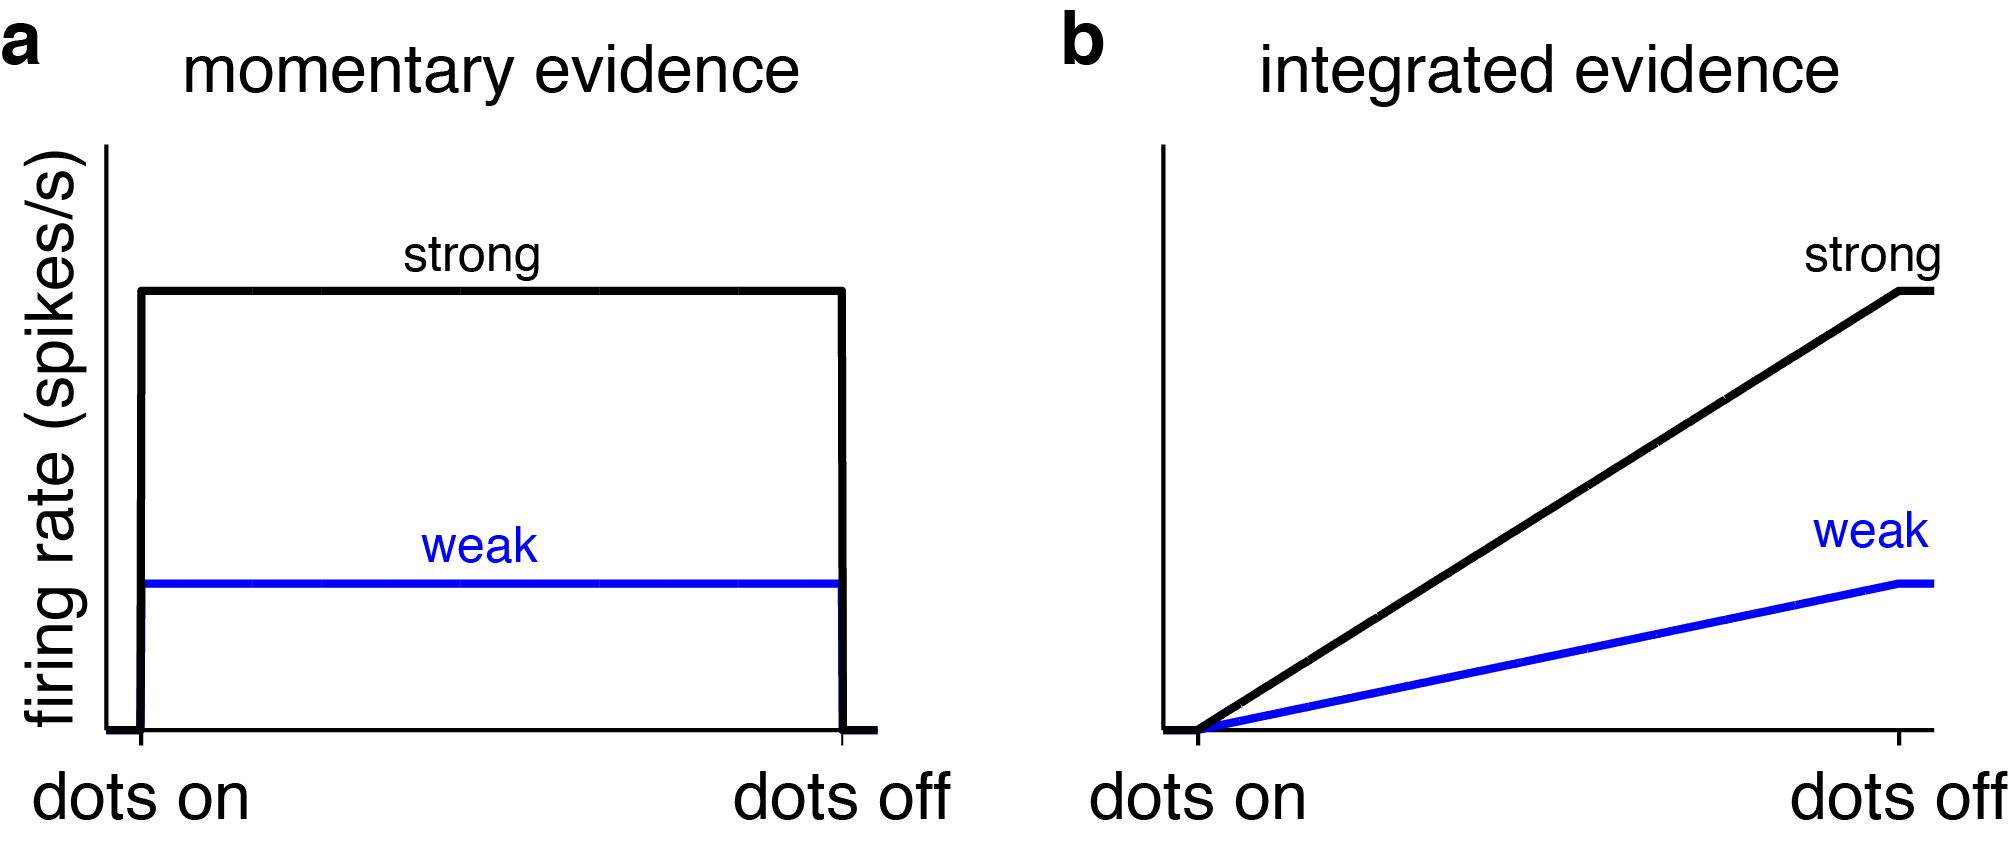
\includegraphics[scale=0.6]{Figures/chapter1/area_MT_LIP_activity_schematic.png}
  \caption[Schematic of Motion Evidence in MT and Integrated Evidence]{\textbf{Schematic of Motion Evidence in MT and Integrated Evidence} The integral (cumulative sum) of the momentary evidence is a ramp-like function reflecting the decision variable. Weak evidence in blue and strong evidence in black.}
   \label{fig:schematic}
\end{figure}
In summary, the standard model proposed by evidence accumulation studies in macaque subjects is that momentary evidence is encoded in area MT (Figure \ref{fig:schematic} a) and the decision variable or integrated evidence is reflected in multiple brain areas including LIP, SC, dlPFC, FEF, and striatum (Figure \ref{fig:schematic} b). Several open questions still remain: for instance, which of the candidate areas reflecting the accumulated evidence are critical to the decision process? How is the accumulation of evidence process implemented? What circuit architecture supports the sensory integration over time? Is the integration of evidence strictly computed by dedicated neurons/areas or is it an emergent property of distributed processing of sensory information?

\section{Evidence Accumulation: Rodent studies}
Addressing these open questions has been challenging in nonhuman primate subjects largely due to the cost and technical constraints. As a result, many scientists have turned to rodents as a complementary model organism for studying the neural circuit mechanism of evidence accumulation. Rodents offer a wide variety of tools for measuring and manipulating neural activity with cell-type specificity. Rodents share a common mammalian ancestor with primates dating back 75-100 million years ago \parencite{Murphy2004} and both species belong to the mammalian superorder \emph{Euarchontoglires}. They possess many of the same brain areas and general brain organization found in primates and humans \parencite{Kaas2009}. The smooth, lissencephalic cortex of rodents is an advantage because brain areas are easily accessible for electrical and optical neural recordings. Rodents also occupy a smaller footprint compared to macaques, and therefore are readily amenable to large-scale studies using numerous subjects. \par 

Although rodents have been trained to perform decision tasks with the random dots stimulus \parencite{Douglas2006,Reinagel2013,Petruno2013,Stirman2016}, recent evidence accumulation studies have introduced discrete pulsatile stimulus sequences. The main advantage of the discrete pulse stimulus is that the evidence at each moment of time and on each trial is known, which is useful when modeling the accumulator value on each trial \parencite{Brunton2013,Hanks2015}. This thesis will focus on tasks using discrete pulsatile sequences.

\subsection{Rats}
Building on the non-humnan primate work in evidence accumulation, several behavioral paradigms have been developed in the rat towards the goal of understanding the neural mechanisms underlying evidence accumulation. \textcite{Raposo2012a} developed a multisensory decision task in which rats were presented with a random sequence of auditory clicks, visual flashes, or both modalities and the rats learned to make a categorical judgment about whether rate of sensory events exceeded a decision boundary. In a parallel study by \textcite{Brunton2013}, rats were presented with two spatially-separate streams of auditory 'Poisson' clicks and learned to make a categorical judgment as to which of the two streams contained more clicks. The same group also developed a separate visual modality version of the 'Poisson' clicks task \parencite{Scott2015SourcesRats}. A third group developed an auditory analog of the random dots task referred to as the 'cloud of tones' task \parencite{Znamenskiy2013b}. In the task, rats judged whether a series ("cloud") of overlapping tones consisted of high-frequency vs. low-frequency tones. \par 

Neural recordings from the rat PPC, at first glance, are consistent with evidence accumulation signatures observed in primate LIP. For example, the firing rates of the neurons in rat PPC exhibit ramp-like activity proportional to the evidence strength \parencite{Raposo2014,Hanks2015}. However, closer inspection of the activity in rat PPC reveal that sensory evidence in accumulated elsewhere \parencite{Hanks2015} and that rat PPC might instead play a role in visual processing \parencite{Licata2017}. Observations from causal manipulation of rat PPC are consistent with the neuropphysiological measurements. Rat PPC activity is not required for performing auditory evidence accumulation \parencite{Raposo2014,Erlich2015}, but it is required for visual evidence accumulation \parencite{Raposo2014,Licata2017}. 

\subsection{Mice}
Mice are an ideal model system for studying neural circuits because of the abundant tools for accessing and probing genetically defined cell types \parencite{Madisen2010,Taniguchi2011,Madisen2012,Madisen2015}. However, in contrast to rats, mice are largely underrepresented in evidence accumulation paradigms, even though mice can be trained to achieve similar levels of performance as rats in perceptual decision-making paradigms \parencite{Douglas2006,Jaramillo2014}. A literature search at the beginning of my thesis research for evidence accumulation tasks in mice yielded only a handful of studies \parencite{Douglas2006,Sanders2012}. \textcite{Douglas2006} trained mice (and rats) to report the direction of random dots by swimming towards a target. This paradigm is not scalable for large cohorts of mice and limits the options for measuring neural activity \emph{in vivo} in behaving animals. In the task developed by \textcite{Sanders2012}, head-fixed mice were trained to report decisions by moving a ball with their paws to the left or the right, depending on which spatial location produced more random pulsatile auditory clicks. This task is well suited for neural measurements, but it is not clear whether large numbers of mice can be trained to successfully perform the task. \par 

Recently, parallel to the work presented in this thesis, several mouse evidence accumulation tasks have emerged \parencite{Stirman2016,Marcos2016,Marbach2016}, reflecting the growing interest in leveraging the benefits of the mouse model for studying neural circuits underlying evidence accumulation. To be clear, I am referring to tasks in which mice are presented with stimuli that vary stochastically across time and therefore require temporal integration (accumulation) of the stimulus to make accurate decisions. Several authors have successfully trained mice on a variety of sensory perception tasks that do not require temporal accumulation of evidence including: 
\parencite{Andermann2010a,Busse2011,Glickfeld2013b,Jaramillo2014,Guo2014b,Burgess2016,Jeong2017}.\par 

It is not established whether mice performing an evidence accumulation task perform as well as the rats trained on the same task or whether mice use the same strategy and/or neural machinery to solve such a task. This thesis will address some of these issues in subsequent chapters. 

% \section{Anatomy of Visual and Parietal Cortices}
% \subsection{Primates}
\section{Definition of Mouse Posterior Parietal Cortex}
PPC is an anatomical region located between somatosensory and visual areas in cortex. It receives inputs from these sensory cortices and projects to frontal motor areas; thus PPC sits at the interface of sensory and motor systems \parencite{Andersen2002}. In primates and humans, this area is greatly expanded and consists of multiple anatomically \parencite{Cavada2001,Cavada1993} and functionally distinct subdivisions \parencite{Andersen2002,Kaas2016} specialized for different actions. Area LIP, discussed previously, is among these PPC subdivisions.\par 

In rodents, the equivalent area referred to as PPC is very narrow strip between primary somatosensory (S1) and visual cortex (V1). Given the relatively small size of the rodent brain and the limited cortical real estate within this strip, it is unclear whether rodents possess a dedicated PPC area. Furthermore, in the mouse, several distinct retinotopic visual areas \parencite{Wang2007} (Figure \ref{fig:vis_areas}a) have been found to reside within the narrow strip. It is not known whether the same is true for the rat, which also have multiple visual areas that surround V1\parencite{Montero1973a,Espinoza1983}. \par 

The most commonly used definition for mouse PPC originates from \textcite{Harvey2012}. Here, PPC was defined based on anatomical projections from an area anterior to primary visual cortex (V1) and posterior to primary somatosensory cortex (S1). Although the anatomical connectivity patterns of their mouse PPC area (Table \ref{table:harveyPPC} ) are similar to those found in nonhuman primate area LIP (Table \ref{table:areaLIP}), the areal extent or boundary of the Harvey et al mouse PPC is not defined, nor is it established whether mouse PPC overlaps with multiple subdivisions as has been observed in primates and rats.\par 

An intriguing hypothesis is that mouse PPC is one or more higher-order visual areas which represent the ancestral (or evolutionary) precursors to PPC found in primates. Candidate higher-order visual areas in the anatomical region between V1 and S1 that qualify as an equivalent PPC area, or subdivision thereof, include areas RL, A, AM, MMA, and RLL. With the exception of MMA and RLL, which were recently discovered \parencite{Zhuang2017}, these areas posses distinct connectivity patterns (input and output) and functional responses to features of grating stimuli \parencite{Andermann2011,Marshel2011,Juavinett2015,Tohmi2014}. These areas also project to frontal motor areas \parencite{Wang2012}, a hallmark feature of sensorimotor areas like PPC \parencite{Kaas2011a}. Furthermore, the functional roles of these higher visual areas in behavior remain unknown. \par

%table generated with http://www.tablesgenerator.com/
\begin{table}
\centering
\begin{tabular}{cl}
\hline
\multicolumn{2}{c}{Areas} \\ \hline
\textbf{Visual} & V1,V2 \\
\textbf{Motor} & M2 \\
\textbf{Frontal} & mPFC, Orbitofrontal \\
\textbf{Limbic} & Cingulate, Retrosplenial, Perirhinal \\
\textbf{Subcortical} & Striatum, Superior Colliculus \\ \hline
\end{tabular}
\caption[Stereotactic Mouse PPC Connectivity Summary]{\textbf{Stereotactic Mouse PPC Connectivity Summary} Anatomical connectivity pattern of mouse PPC defined by \textcite{Harvey2012}.}
\label{table:harveyPPC}
\end{table}

\begin{table}
\centering
\begin{tabular}{cl}
\hline
\multicolumn{2}{c}{Areas} \\ \hline
\textbf{Visual} & \begin{tabular}[c]{@{}l@{}}MT, FST, STP, IT, V2, \\ V3, V4, PO\end{tabular} \\
\textbf{Motor} & FEF, Premotor \\
\textbf{Frontal} & Prefontal Cortex, Orbitofrontal \\
\textbf{Limbic} & \begin{tabular}[c]{@{}l@{}}Cingulate, Retrosplenial,\\ Presubiculum, Perirhinal\end{tabular} \\
\textbf{Subcortical} & Striatum, Superior Colliculus, Pons \\ \hline
\end{tabular}
\caption[Area LIP Projections Summary]{\textbf{Area LIP Projections Summary} Cortical and Subcortical projections from area LIP \parencite{Cavada1989a,Cavada1989c,Cavada2001} MT, medial temporal area; FST, fundal superior temporal area; STP, superior temporal polysensory area; IT, inferior temporal cortex; V2, visual area 2; V3, visual area 3; V4, visual area 4; PO, parieto-occipital area; FEF, frontal eye field.}
\label{table:areaLIP}
\end{table}

%------------------------------------------------------------------
\begin{figure}
\centering
  	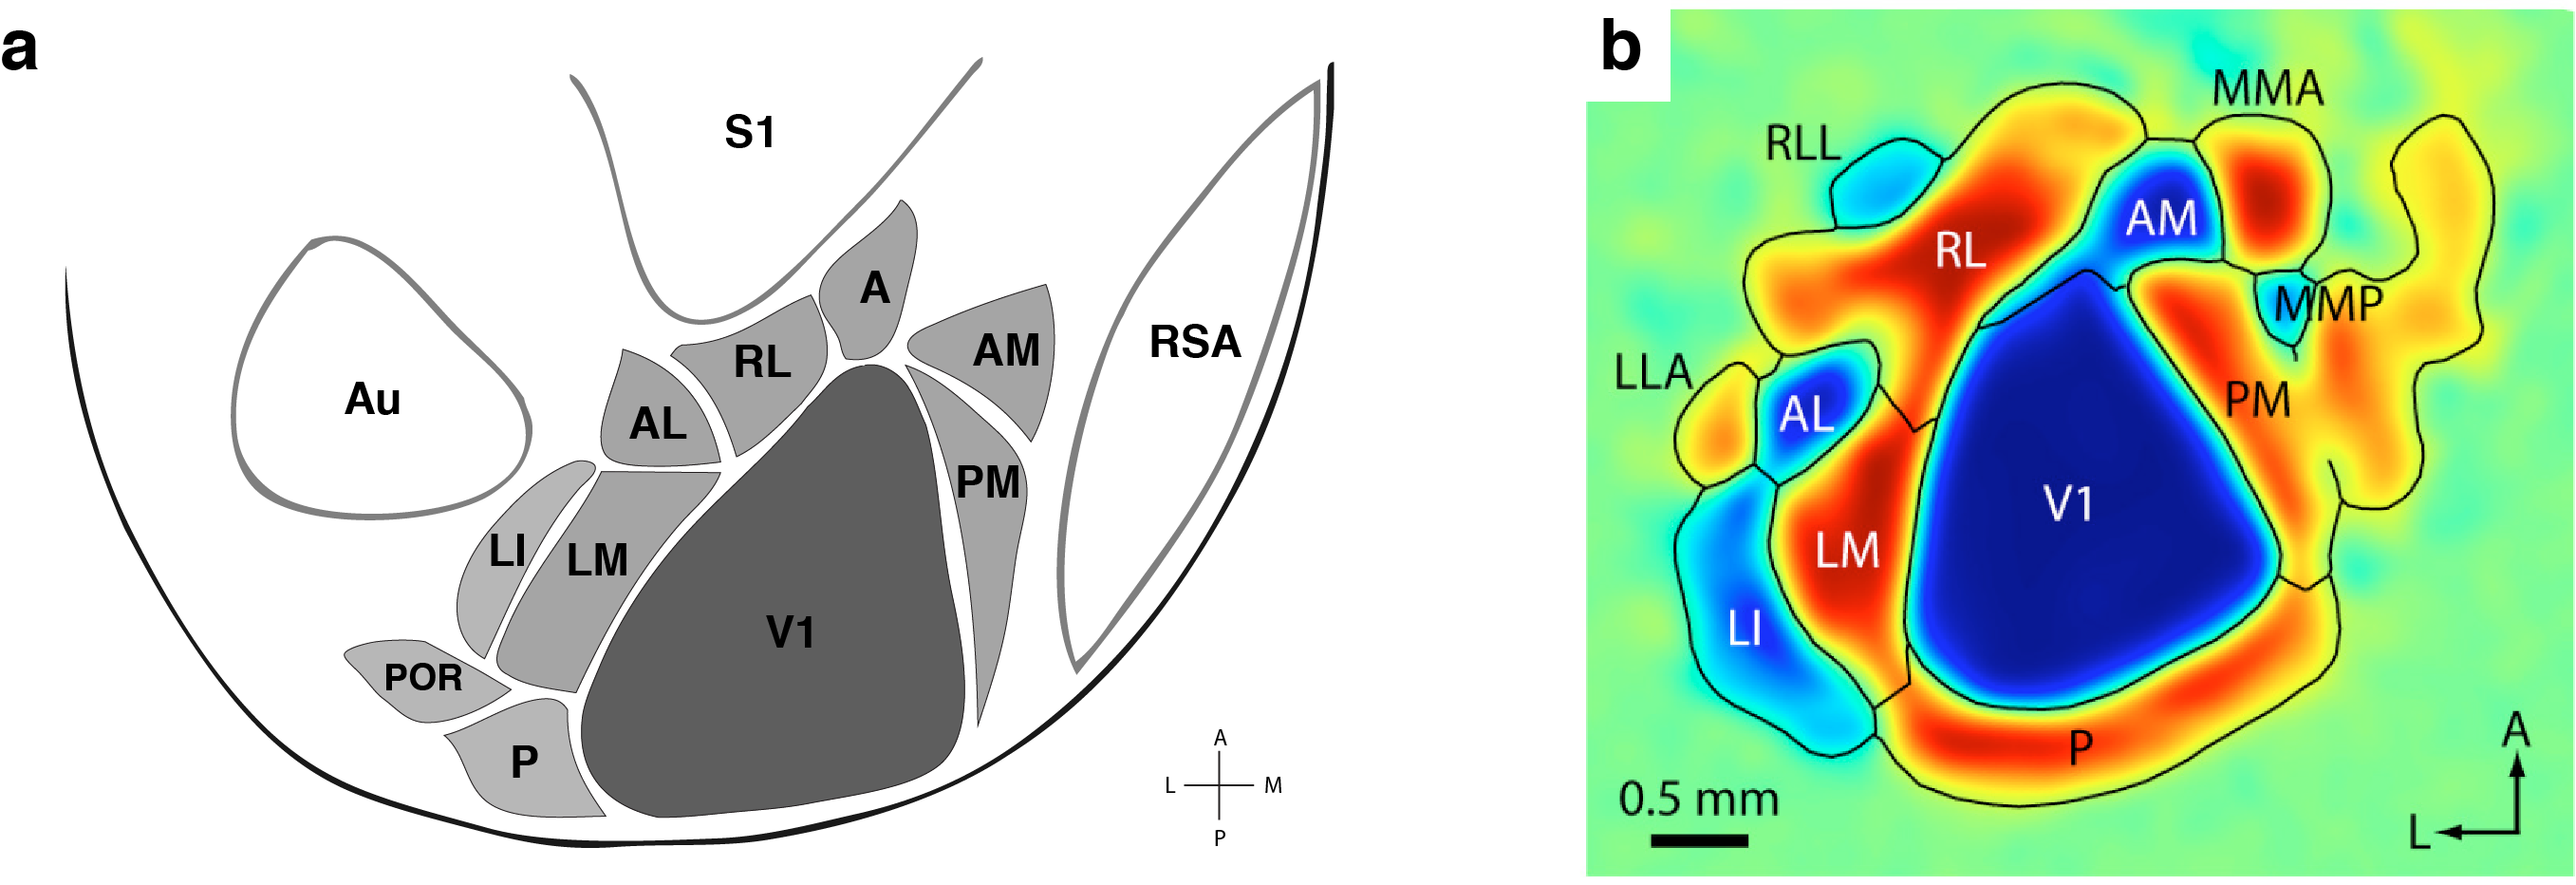
\includegraphics[width=\textwidth]{Figures/chapter1/visual_areas_map.png}
  \caption[Mouse Visual Cortex and the Surrounding Areas]{\textbf{Mouse Visual Cortex and the Surrounding Areas} (a) Schematic of the original nine secondary visual areas identified by \textcite{Wang2007} in light gray. (b) The extended retinotopic map based on widefield calcium imaging by \textcite{Zhuang2017} includes additional areas not present in the original map (a).} 
   \label{fig:vis_areas}
\end{figure}

\section{Thesis Outline}
Due to the vast genetic tools available, mice are currently a superior model organism for casual studies examining the role of brain areas and neural activity in the accumulation of sensory evidence and production of behavior. However, the usefulness of mice in studies of perceptual decision making, and in particular evidence accumulation, is limited by current lack of knowledge concerning whether mice can learn accumulation tasks and the anatomy/connectivity of mouse sensory and decision making areas. This thesis aims to address this paucity of knowledge. \par 

In Chapter \ref{Chapter2}, I describe the psychophysical paradigm for investigating evidence accumulation in mice and provides quantitative description of the mouse behavior. In Chapter \ref{Chapter3}, I describe causal manipulation experiments of mouse PPC defined by stereotactic coordinates provided by \textcite{Harvey2012} in order to address the role for a putative mouse PPC homologue in evidence accumulation. In Chapter \ref{Chapter4}, I discuss experiments aimed at targeting a secondary visual area and putative subdivision of mouse PPC, area AM, for inactivation during visual evidence accumulation. Finally, in Chapter \ref{Chapter5}, I discuss results of analyses that reveal insights about how mice process natural scene images, forming the basis for an understanding of how mice may use sensory information to guide decisions.



\chapter{Visual Flashes Categorization Task} % Main chapter title
\label{Chapter2} % 
One of the main goals of the thesis was to develop a psychophysical task for studying visual evidence accumulation in mice. When I first began work on the thesis project, there were hardly any existing paradigms for training mice in accumulation of evidence tasks. I adopted the behavioral template used in the Churchland lab and several other labs for training freely-moving rats on sensory accumulation tasks as discussed in Chapter \ref{Chapter1}. The main requirement was to have precise temporal control over stimulus presentation and delivery. I used a randomized sequence of flashes delivered from a full-field LED panel at a fixed location. The non-spatial nature of the stimulus was incorporated to decouple the sensory stimulus location from the lateral movements of the mouse when reporting its decision. \par 
Mice were trained to categorize a sequence of visual flashes based on whether the total number of flashes exceeded an experimenter-determined category boundary. In this chapter, I will describe the behavioral paradigm and provide quantitative description of the psychophysical behavior on the task. The first part of the chapter describes the pulsatile visual stimuli and the behavioral training approach. The second part of the chapter discusses quantitative analyses of the  psychophysical behavior of the mice. \par 
\section{Visual Pulsatile Stimuli} 
In the initial experiments in the thesis, I began training mice with a pulsatile stimulus developed in the Churchland lab for studying multisensory integration \parencite{Raposo2012a}. The pulsatile stimulus, which I will refer to as bimodal interval stimulus, consisted of 15 ms flashes of light with fixed inter-flash intervals of 50 or 100 ms. The mouse PPC disruption study presented in Chapter \ref{Chapter3} used the bimodal interval stimulus. A drawback of the bimodal interval stimulus is that the stimulus space is very limited. The fixed interval stimulus only ranges from 9 to 16 flashes/s, and at the extremes the inter-flash intervals were either 100 ms or 50 ms. Thus, the number of possible ways to produce a given sequence of pulses was limited or redundant (Figure \ref{fig:combo}a). \par 

To increase the richness of the pulsatile sequence, I implemented a stimulus with variable inter-flash intervals analogous to the stimulus developed by \textcite{Brunton2013} and \textcite{Scott2015SourcesRats}. This pulsatile stimulus consisted of 20 ms flashes, with inter-flash intervals which followed a gamma distribution (Figure \ref{fig:combo}b). The arrival of each pulse is random and varies across trials of the same flash rate. This allows for a wide variety of pulsatile sequences for a given flash rate (Figure \ref{fig:combo} a). For the exponential interval distribution, there are at least three orders of magnitude more possible stimulus combinations than the fixed interval task. The minimum inter-flash interval is 20 ms, and the maximum interval is determined by the number of flashes for a given stimulus. 
% To generate the stimulus, time was discretized into 25 20 ms bins, and in each of the bins Poisson coin was flipped to assign a flash in that bin. Each of the 25 bins was followed by an empty 20ms bin, where no flash occurred. Hence there was a total of 50 bins, 20ms each, resulting in 1000ms fixed stimulus duration. 

\begin{figure}
\centering
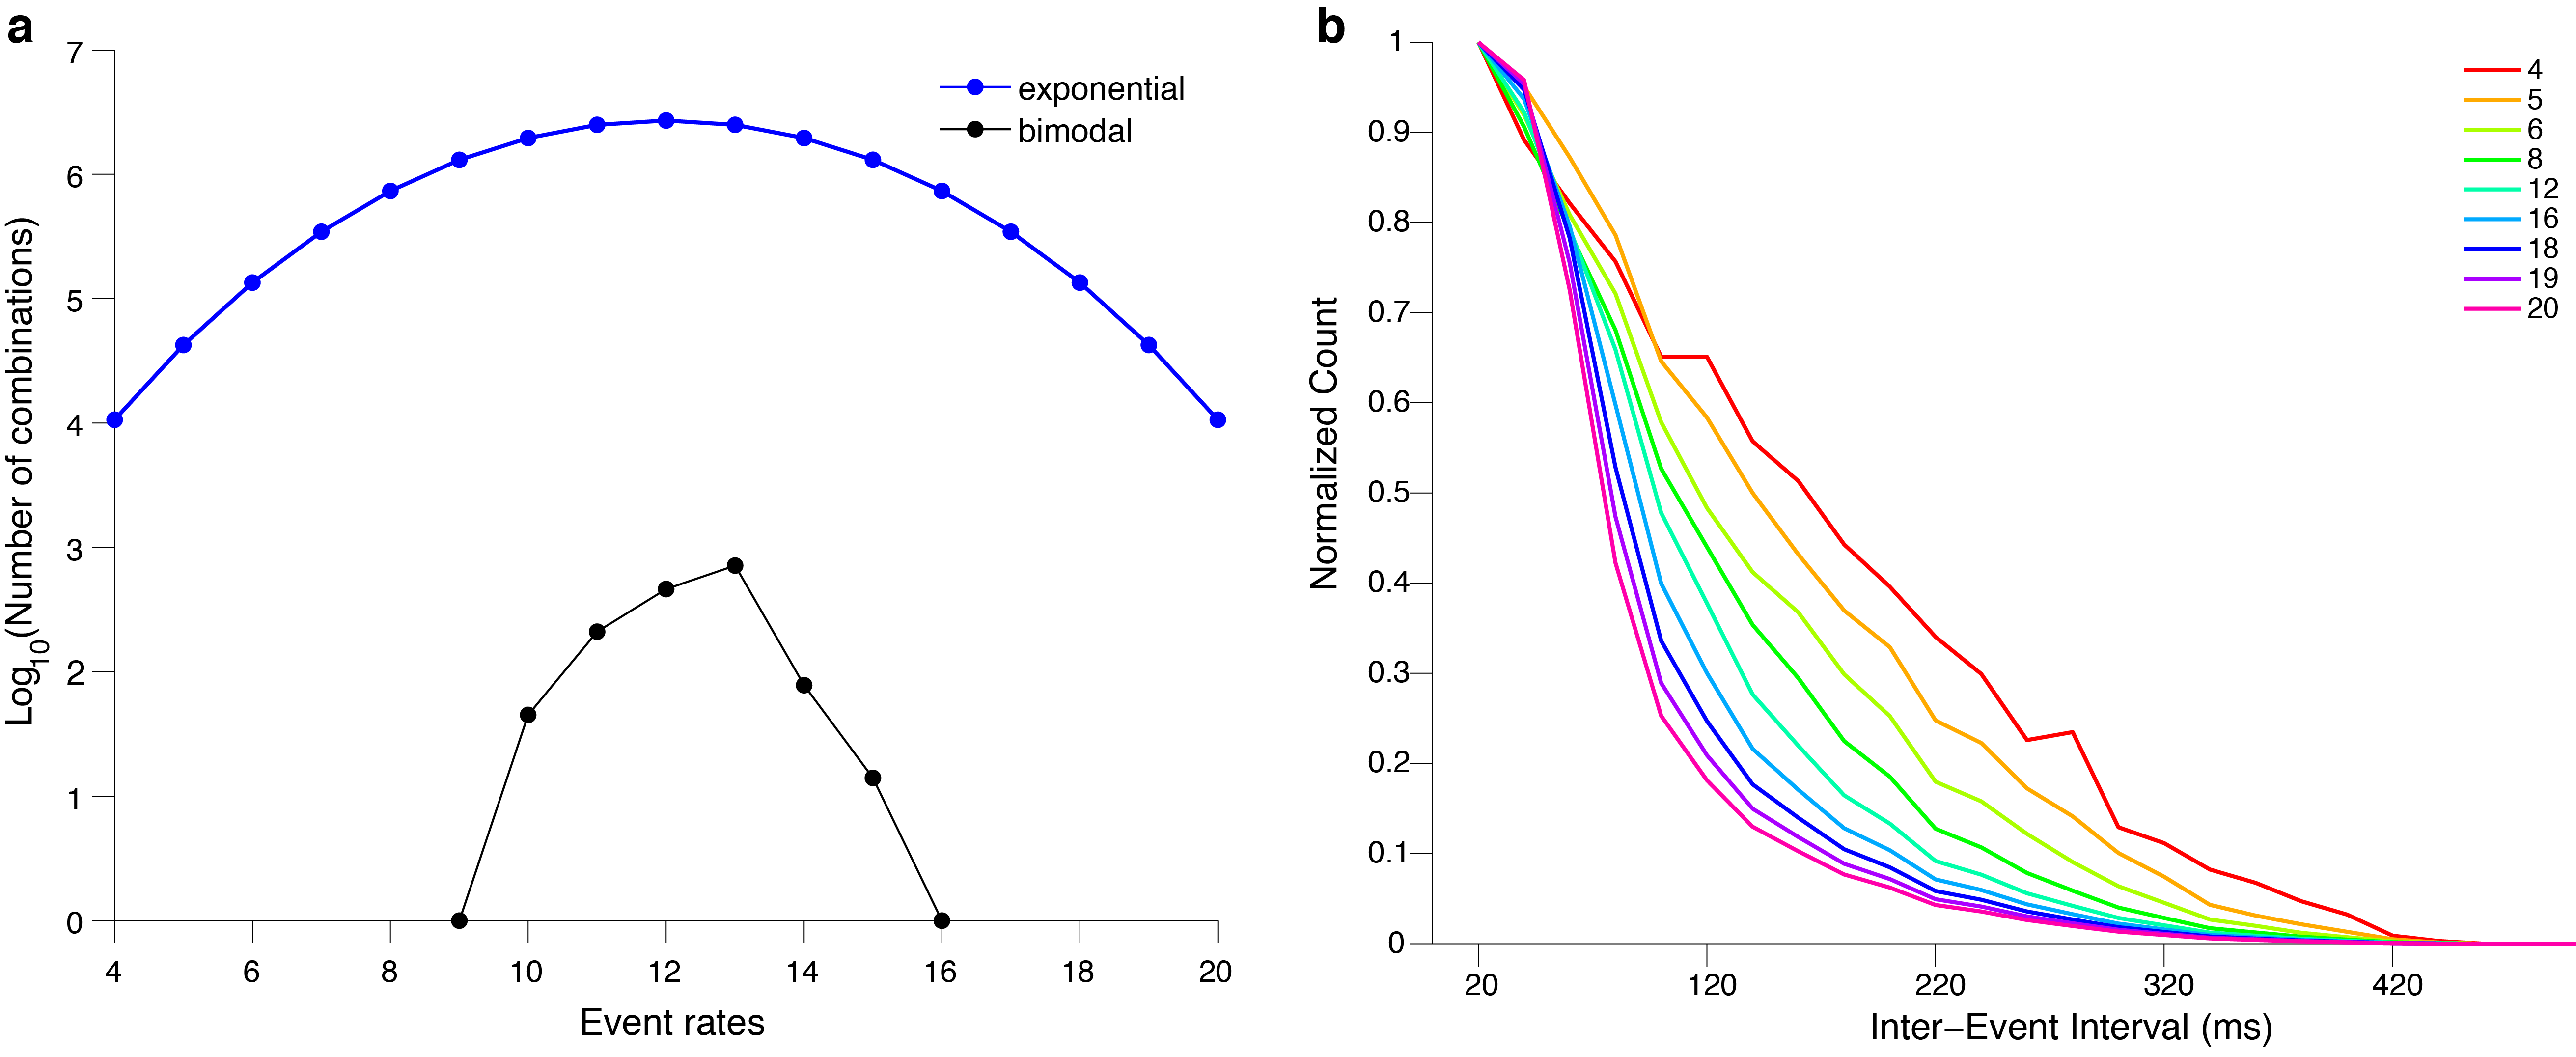
\includegraphics[width=\textwidth] {Figures/chapter2/combo_and_intervals.png}
\caption[Number of possible configurations per flash-rate and histogram of inter-pulse interval]{\textbf{Number of possible configurations per flash rate and histogram of inter-pulse intervals} (a) Comparison of the number of unique pulsatile sequences for each flash rate for the bimodal (black) and exponential interval (blue) pulsatile sequences. (b) Histogram of inter-flash intervals for each flash count in the exponential interval stimulus.}
  \label{fig:combo}\label{fig:stimulusprop}
\end{figure}
%----------------------------------------------------------------------
%----------------------------------------------------------------------
\section{Task Structure}
The behavioral task was performed in a three-port choice box \parencite{Uchida2003}. Mice were trained to self-initiate trials by poking into the center port and maintaining fixation within the center port for up to 1100 ms, while the visual stimulus played (Figure \ref{fig:taskstructure}). At the end of the wait period, an auditory go cue was delivered to inform the subject to make a response. The mice were trained to respond to the right-hand port if the number of flashes exceeded 12 flashes/s (high-rate), and to the left-hand port if the number of flashes was less than 12 flashes/s (low-rate). Mice were given a liquid reward (2-4 $\mu$L of water) for correct responses. Incorrect responses and breaks in center-port fixation were punished with a timeout period of 2-4s, in which the mouse was not allowed to initiate a trial. 
\begin{figure}
  \centering
  	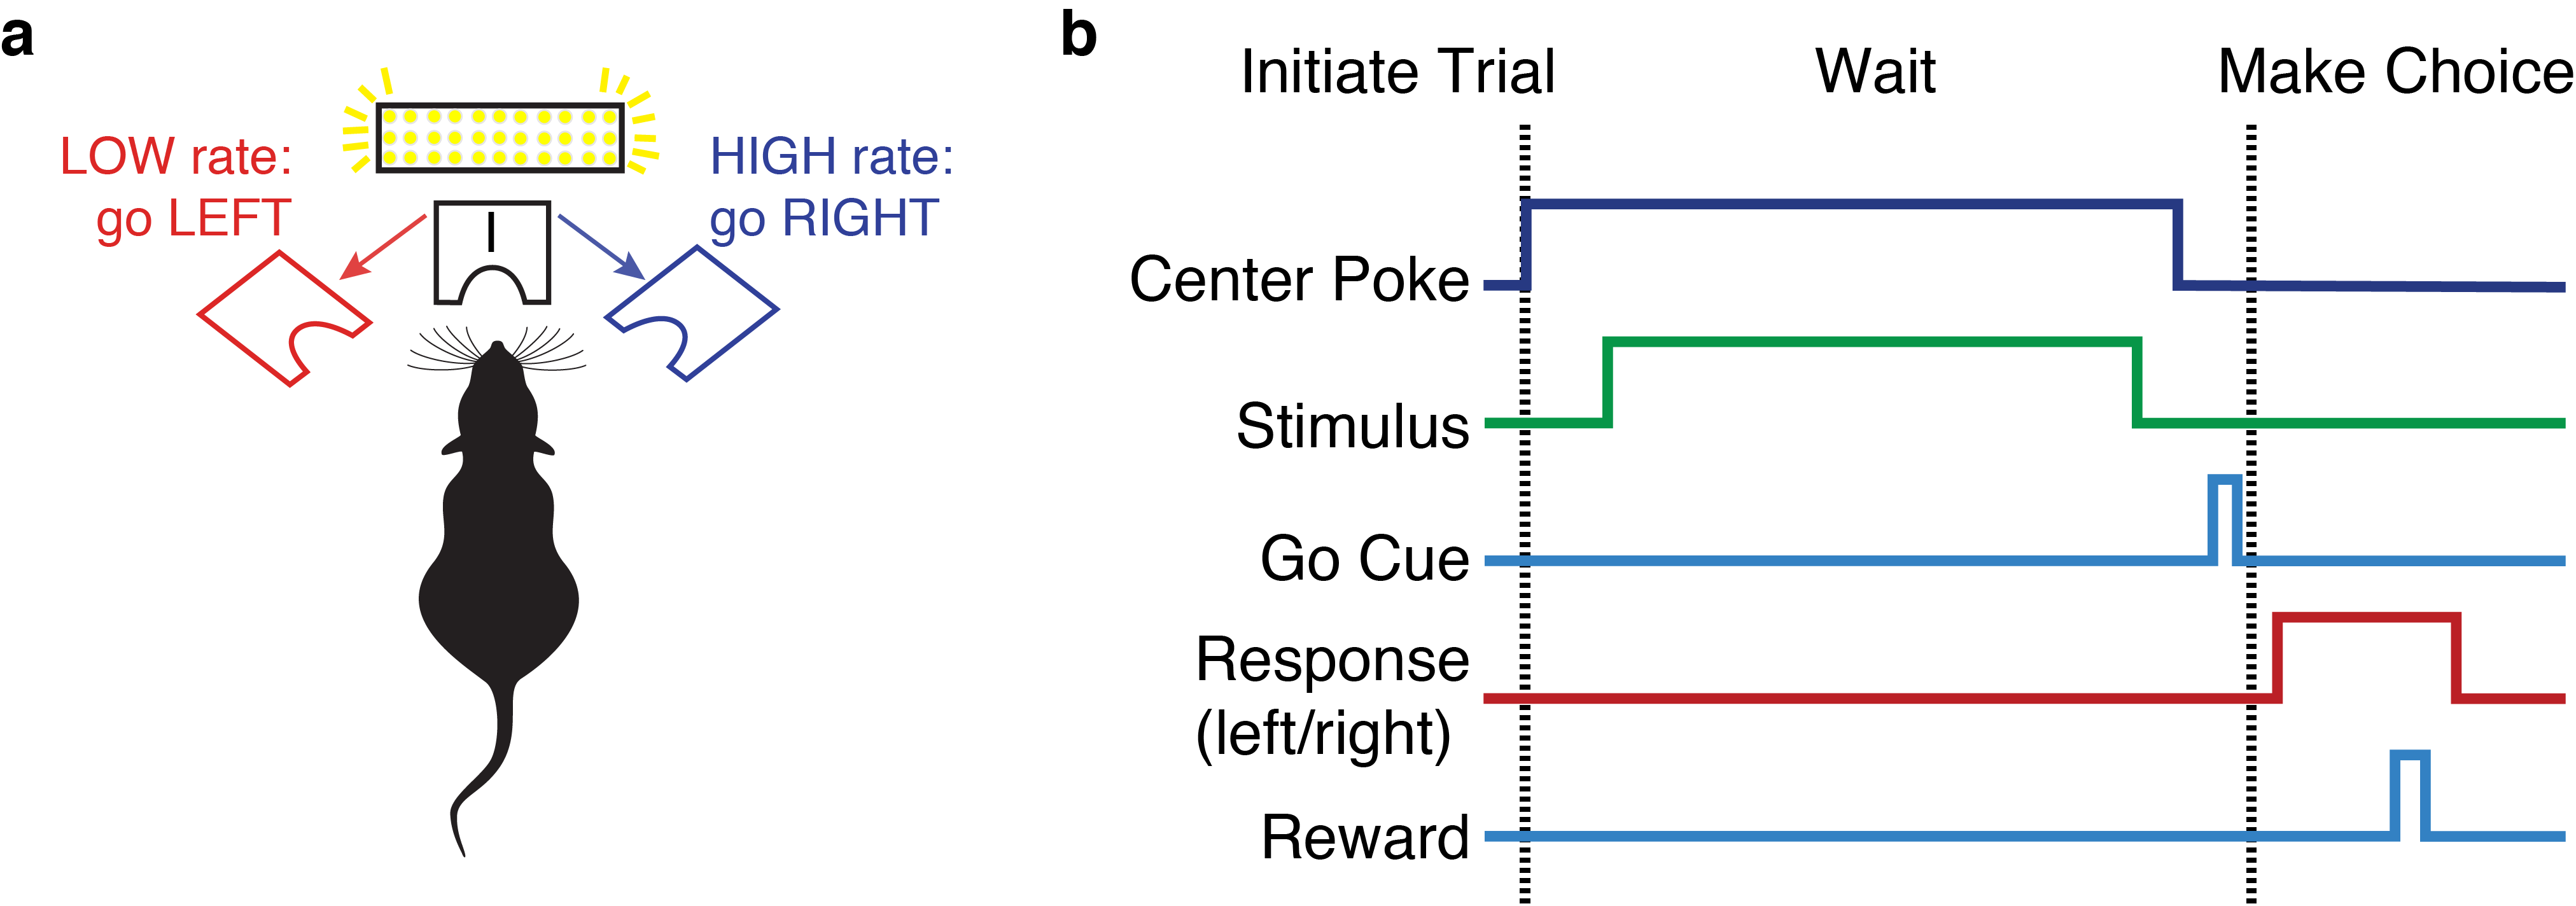
\includegraphics[width=\textwidth]{Figures/chapter2/taskstructure.png}
  \caption[Task Structure]{\textbf{Task Schematic and Trial Structure}. a) Three-port choice task schematic. The mouse initiates trials and stimulus delivery by poking the center port. The mouse responds to whether the stimulus is low-rate (left port) or high-rate (right port). (b) The mouse has to wait at the center port for at least 1100 ms, the stimulus is delivered after a variable delay (10-100ms). At the end of the 1000ms stimulus period, an auditory "Go" tone is played to inform the subject to make a choice. Correct choices to the left or right are rewarded with a small drop of water (2 $\mu$L), incorrect choices earn the subject a 2-3 s timeout.}
   \label{fig:taskstructure}
\end{figure}
%----------------------------------------------------------------------
%----------------------------------------------------------------------
\section{Behavioral Training}
Mice were trained in a semi-automated fashion. The task trial type, stimulus delivery, reward/punishment delivery, and the subjects' responses on each trial were determined and/or recorded by a finite state machine running on an Arduino-based system (Bpod, SanWorks LLC). The subjects' performance was  monitored during each session and occasional intervention was required to shape the behavior, including countering severe side biases or increasing/decreasing the difficulty levels. \par 
Mice performed several hundreds of trials per session (Figure \ref{fig:numTrials}) and acquired the easiest level of the task in less than 20 sessions or 10,000 trials (Figure \ref{fig:pcorrect}). Behavioral training typically lasted for 2-3 months depending on the mice. The mice were trained daily (5 days/week) for up to 2 hours per session.\par 
\begin{figure}
  \centering
  	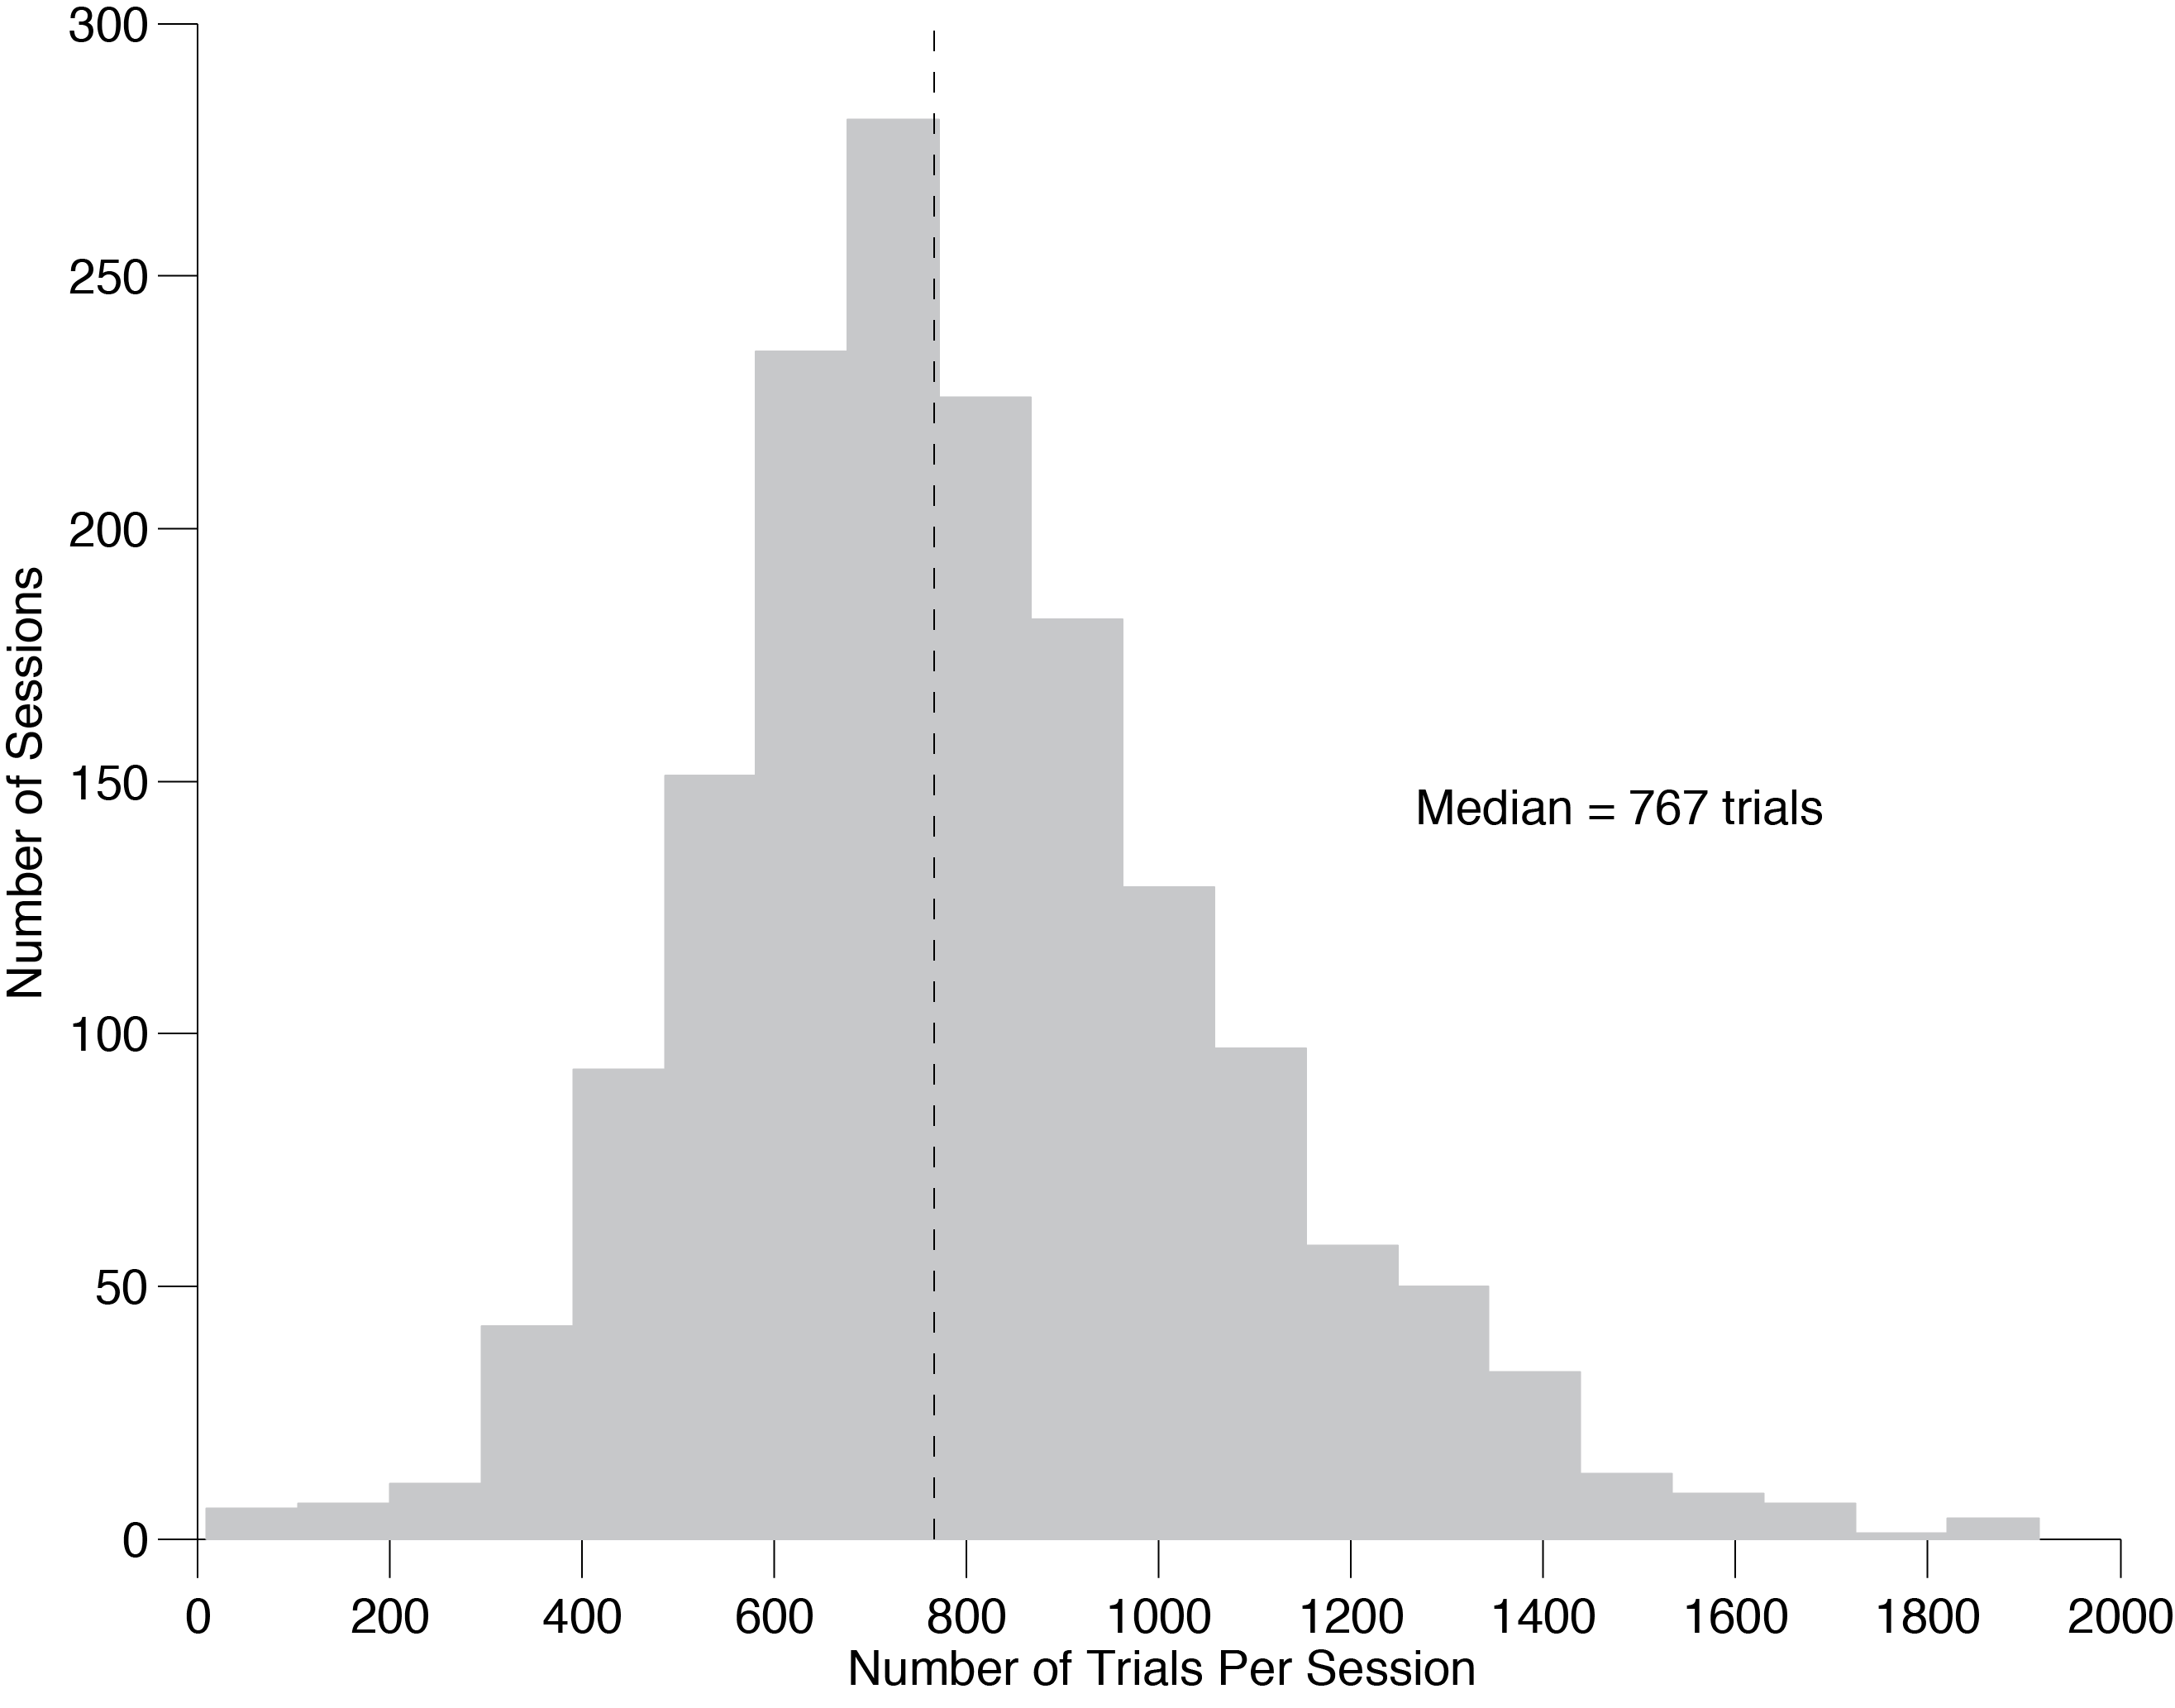
\includegraphics[width=\textwidth]{Figures/chapter2/NumTrialsPerSessions24mice.png}
  \caption[Number of Trials Per Session]{\textbf{Number of Trials Per Session}. Mice performed hundreds of trials per session. n = 24 mice.}
   \label{fig:numTrials}
\end{figure}

The first stage of training was to teach the mice to wait at the center port for at least 1100 ms. This was done by gradually increasing the minimum required wait duration from 25 to 1100ms, by an increment of 0.1 ms on every trial. With this approach, it took the mice about 10-12 sessions to learn to wait for at least 1000 ms (Figure \ref{fig:completeRate} a). During this phase, mice were not rewarded for making the correct association between the stimulus and response port; rather on each trial, a random port (left or right) was chosen as the reward port and a liquid reward was delivered to the port. I found that the number of sessions it took the mice to learn center fixation can be reduced significantly (by a factor of 5), by additionally rewarding the mice at the center port (0.5 $\mu$L) each time they waited the minimum required center wait duration (Figure \ref{fig:completeRate} c). Trials in which the mouse waited the minimum required duration at the center port we refer to as completed trials. Mice rewarded at the center port achieved a completion rate above 90\% compared to mice not rewarded at the center port.\par
%Learning rate multiple mice
\begin{figure}
  \centering
  	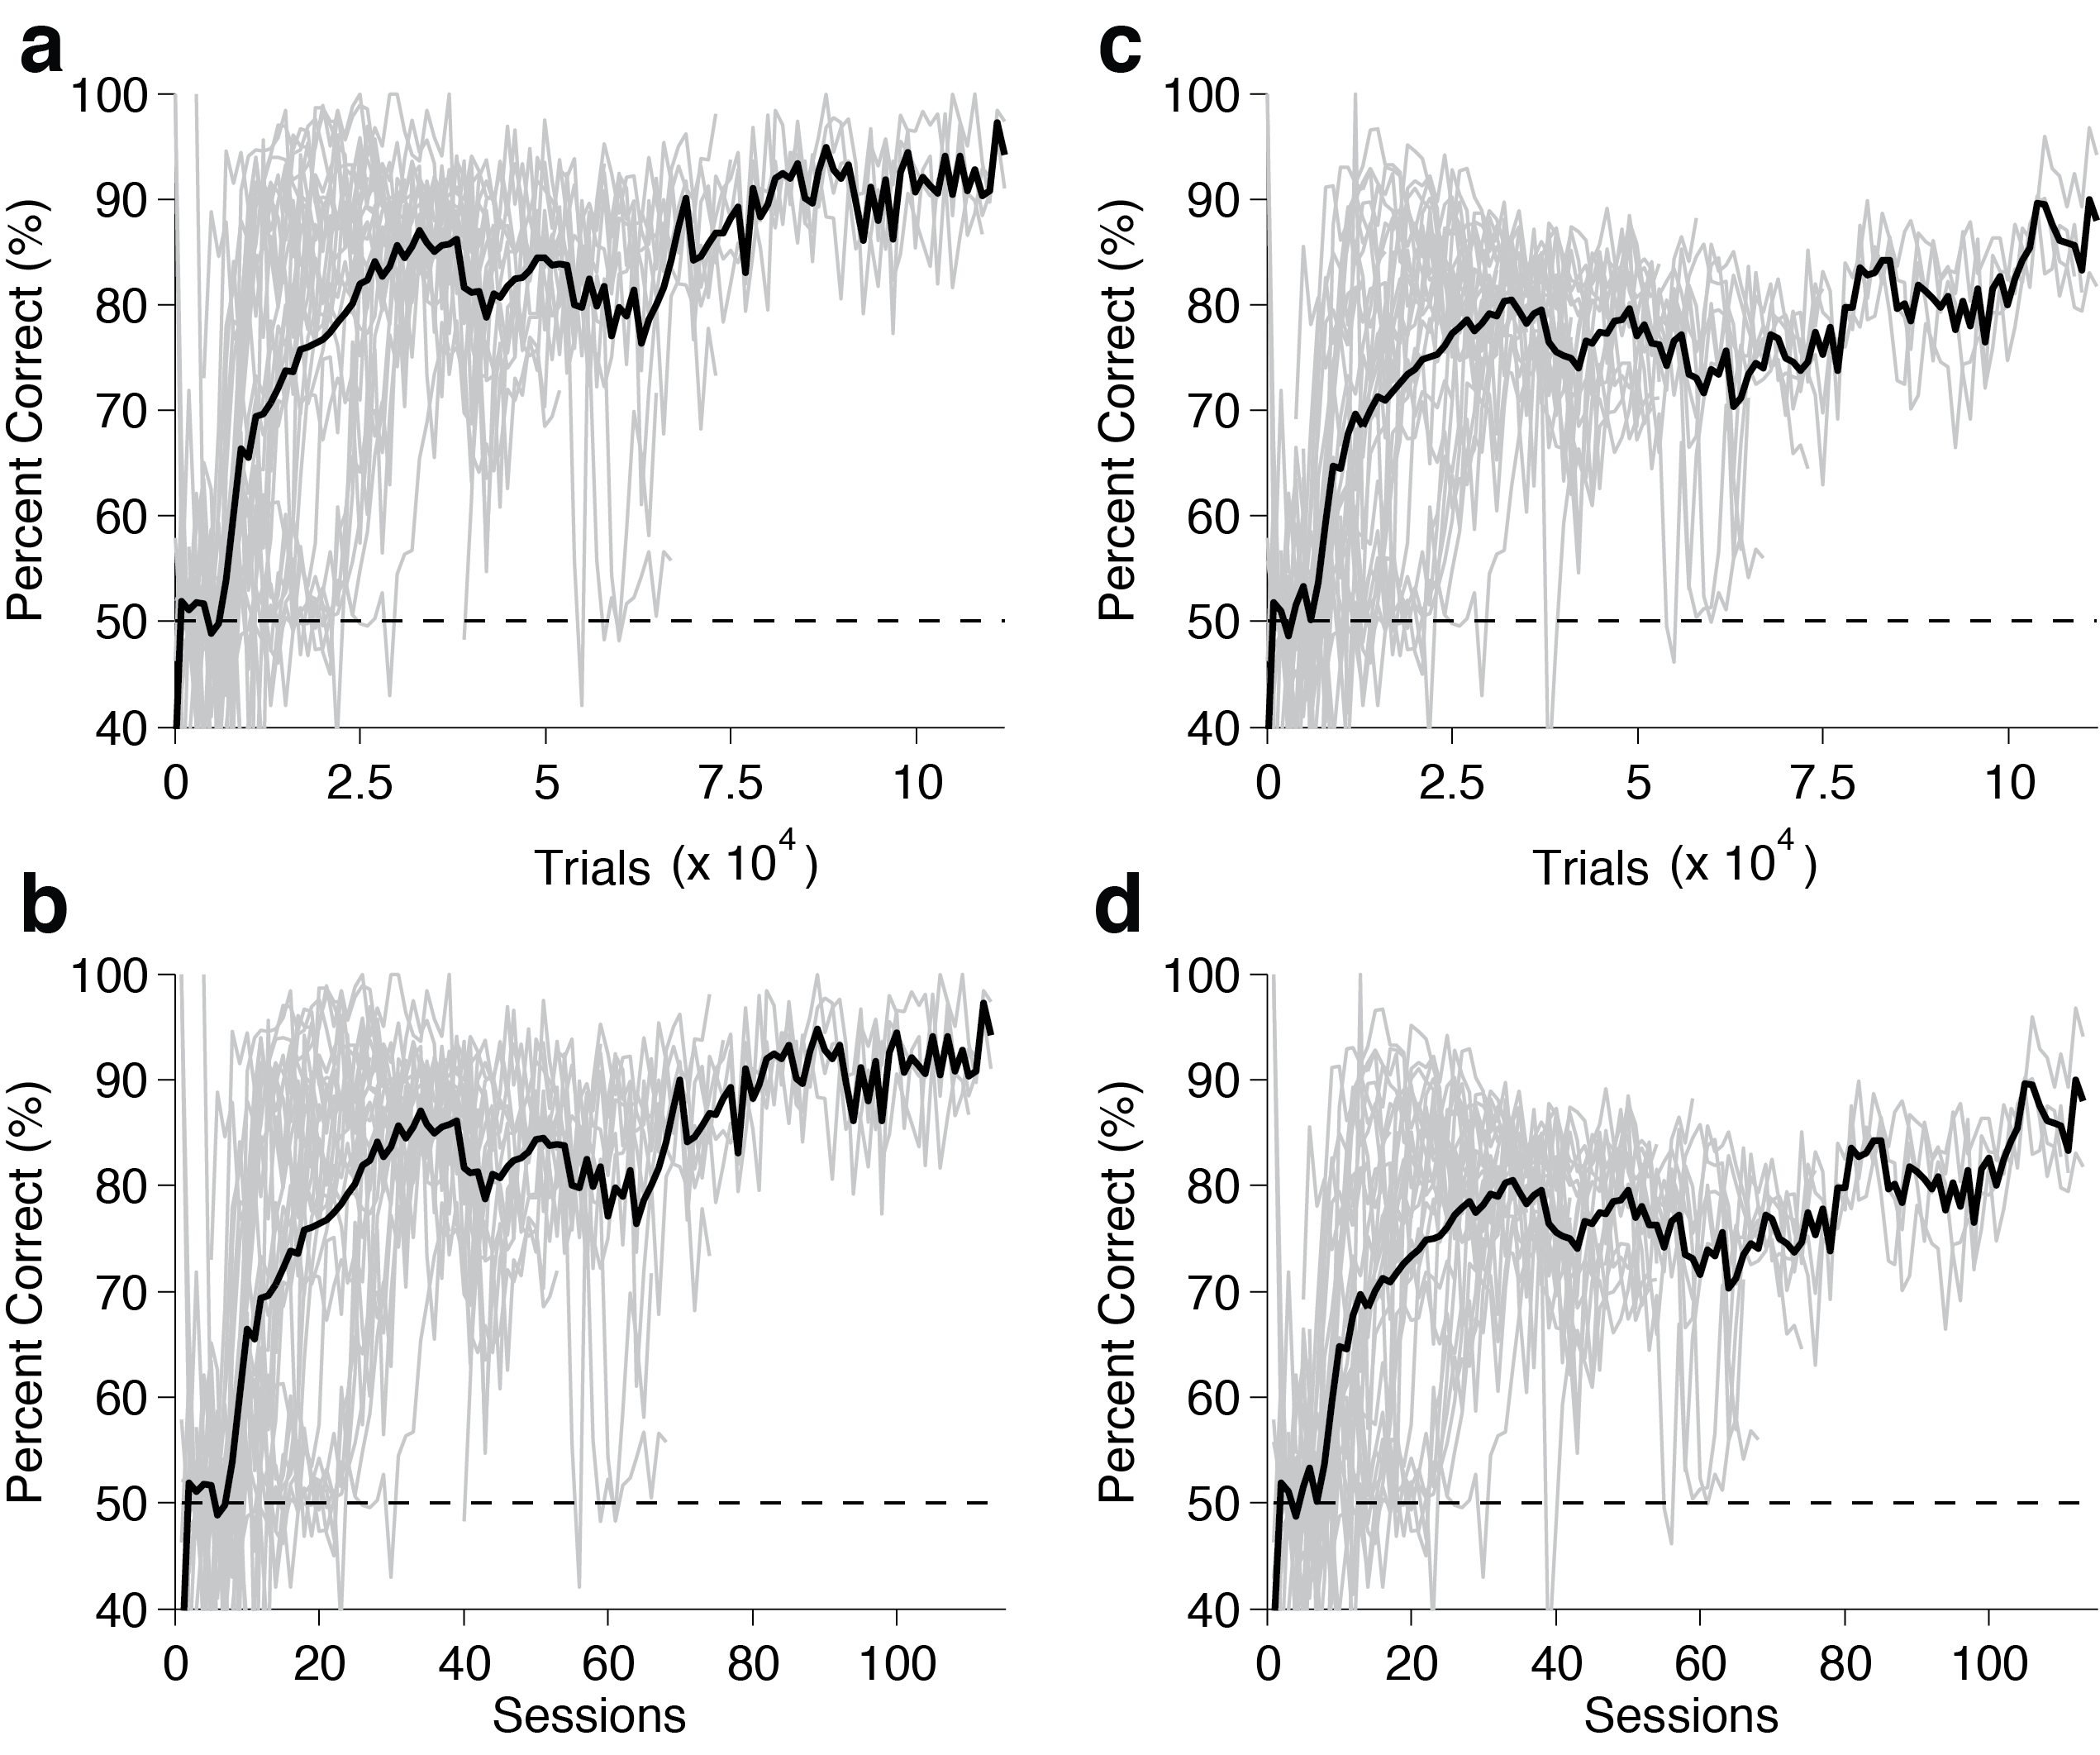
\includegraphics[width=\textwidth]{Figures/chapter2/percentCorrectAllMice.png}
  \caption[Learning Rate]{\textbf{Learning Rate of Multiple Mice.} (a) Percent correct on easiest stimulus conditions (4 and 20 flashes/s) and (c) Percent correct on all stimulus conditions plotted across trials and sessions. Gray traces are individual mice. Black trace, average across mice (n = 24 mice).}
   \label{fig:pcorrect}
\end{figure}
In the second stage of training mice were trained to associate high-rate flashes (>12 flashes/s) with the right-hand port and low-rate flashes (< 12 flashes/s) with the left-hand port. For some mice, the contingency was reversed, such that high-rate flashes were rewarded at the left-hand port and low-rate flashes were rewarded at the right-hand port. The mice learned this phase by trial and error. They were rewarded for making the correct association and punished with a time-out period for incorrect responses. Trials with flash rates of 12 flashes/s were randomly rewarded on the left or right hand port. During this phase, mice typically developed strong side biases, for instance always going to the right-hand port. Depending on the severity of the bias, one of several strategies for countering the bias was used including adjusting the reward volumes/ratio on the left vs right port, adjusting the proportion of left vs right trials, and/or physically blocking access to the biased port. We also made use of custom written antibias software in the lab to handle minor cases of bias. \par 
\begin{figure}
  \centering
  	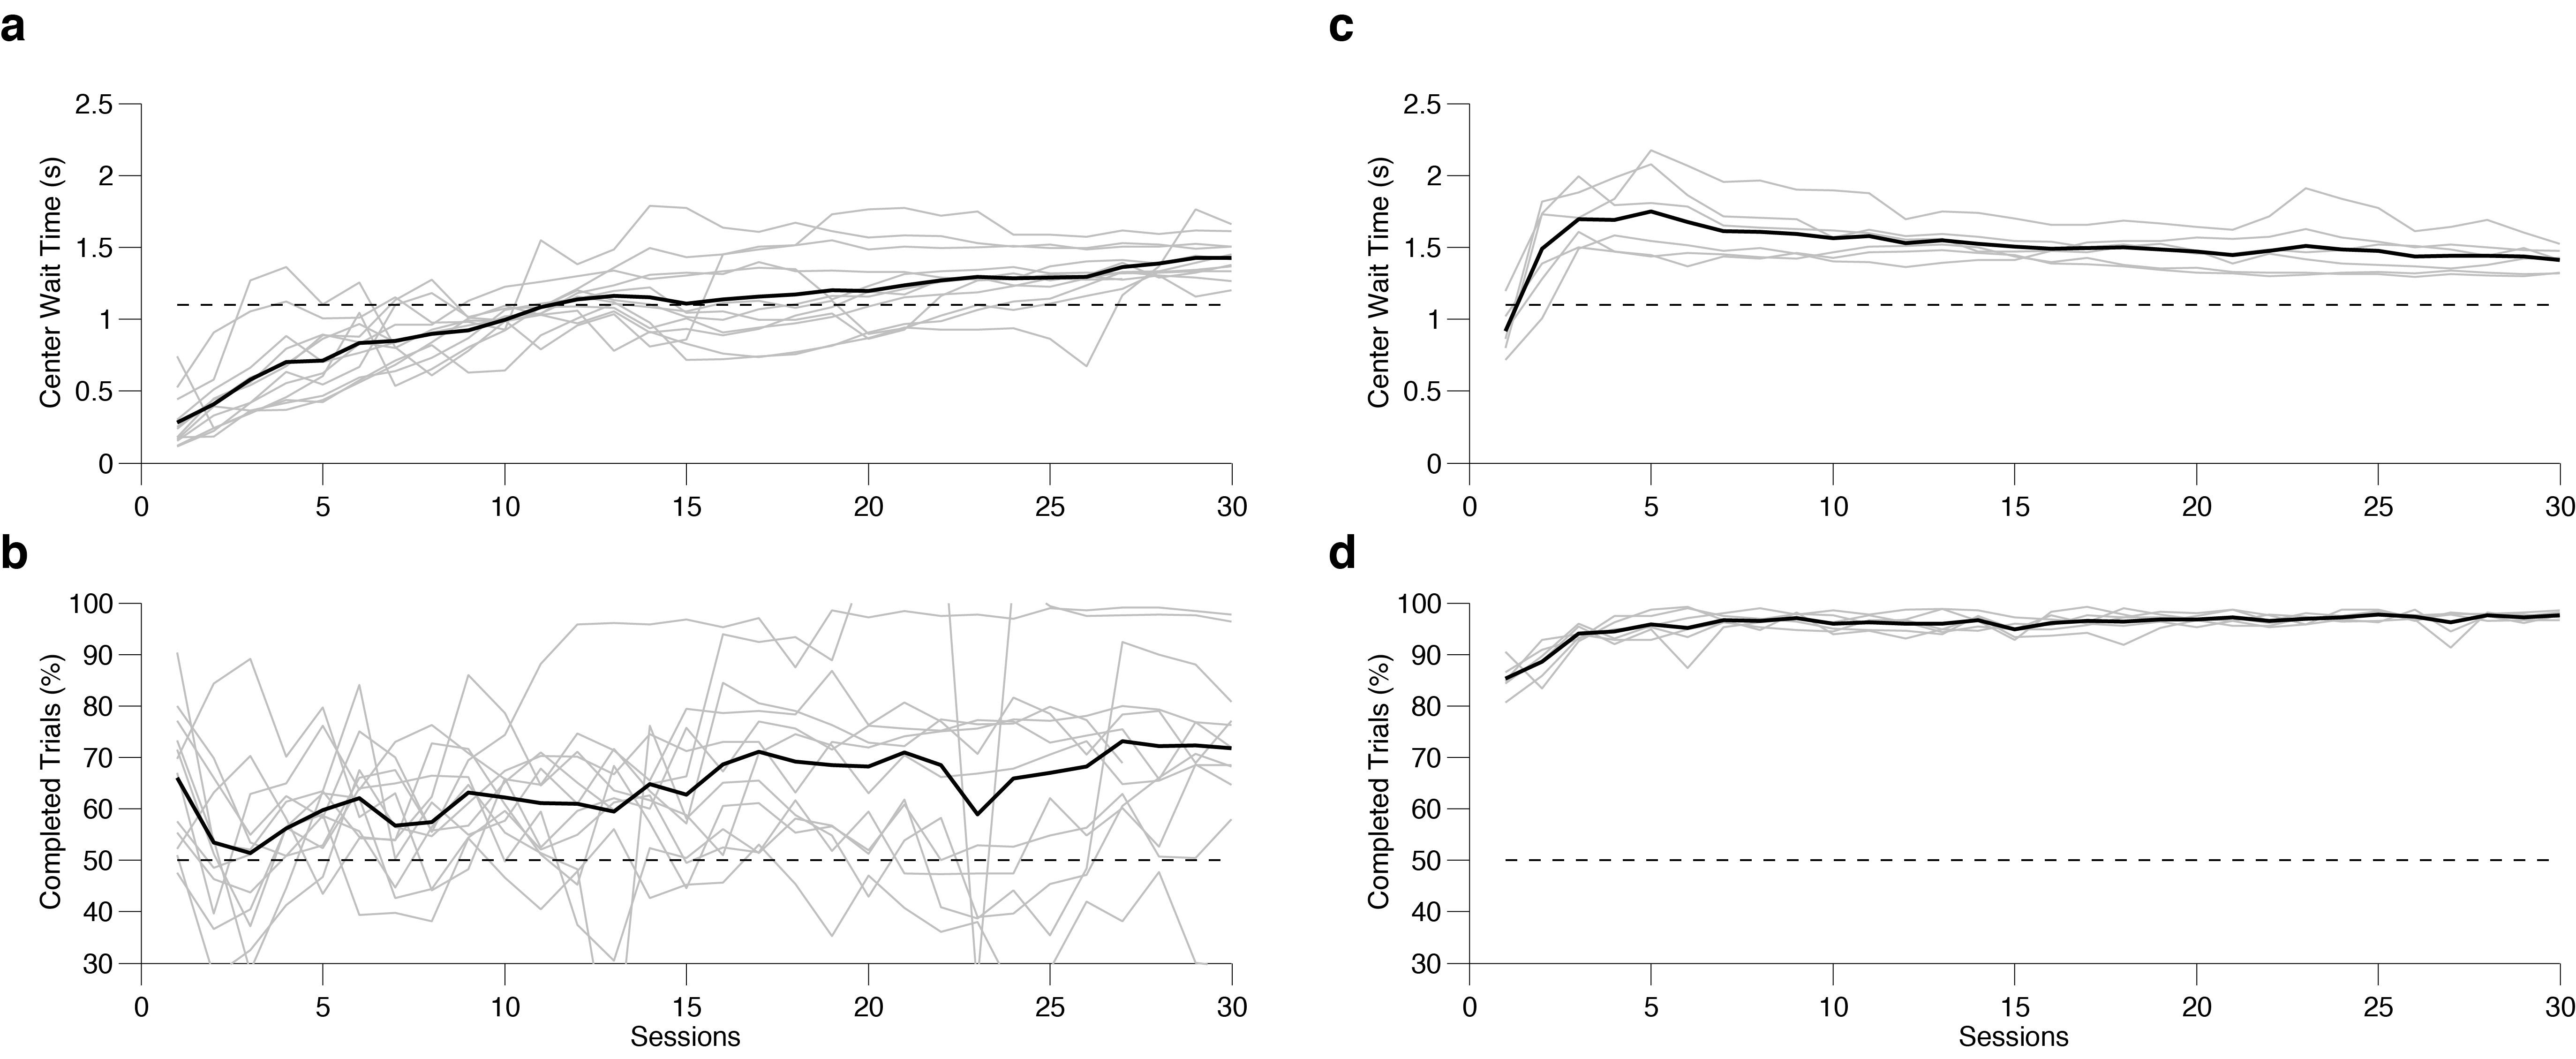
\includegraphics[width=\textwidth]{Figures/chapter2/CenterWaitTimeandCompletionRateComparison.png}
  \caption[Median Center Wait Duration and Trial Completion Rate]{\textbf{Median Center Fixation and Trial Completion Rate.} Comparison between (a,b) Mice that were not rewarded at the center (n = 12) (c-d) Mice rewarded at the center port (n = 6). Gray traces, individual mice. Black trace, average mouse.}
   \label{fig:completeRate}
\end{figure}
In the first two phases, the mice were presented with the easy flash rates at the extremes of the stimulus range (4, 5, 19 \& 20 flashes/s). As the mice improved in performance,  flash rates closer to the category boundary (12 flashes/s) were gradually introduced. For symmetry, rates were introduced in pairs (eg. 4 \& 20, 5 \& 19, 6 \& 18, 8 \& 18 etc). Mice initially had trouble achieving high performance with only 1000 ms of stimulus. To help them during training, the stimulus was extended beyond 1000 ms by repeating the same stimulus sequence for an additional 1000 ms. The extended portion of the stimulus was gradually reduced over the course of training. A fully trained mouse experiences at least 6 pairs of flash rates and waits for at least 1100 ms at the center port. This criteria typically takes at least 1 month to achieve. In 2-3 months, trained mice can experience the entire range of flash rates without the extended stimulus.
%--------------------------------------------------------------------
\section{Psychometric Performance}
The subject's performance on the task is quantified with a psychometric function (Figure \ref{fig:pmfs}). The psychometric function is a quantitative description of the relationship between stimulus features and the subject's choices on a psychophysical paradigm and is used as an inference model of the underlying perceptual mechanism used to perform the discrimination task. While the true underlying function used by the subjects to solve the task is unknown \parencite{Kingdom2010}, typically psychometric curves are generated by fitting a sigmoidal function such as the logistic function or cumulative Gaussian \parencite{Wichmann2001}. In general, for the data in this thesis, we fit the psychometric curve using either logistic or cumulative Gaussian function. Both functions fit the data similarly.\par 
For the visual pulses discrimination task, the general form of the psychometric function defines the probability (\emph{$p_h$}) that the subject chooses the port associated with high flash rates as:
\begin{equation}
	\centering
	p_h = \gamma + (1-\gamma - \lambda)F(x;\alpha,\beta)
\end{equation}
where $\gamma$ and $\lambda$ are the lower and upper asymptote of the psychometric function, which parameterize the guess rate and lapse rate, respectively; \emph{F} is a sigmoidal function, in our case either the logistic function or cumulative Normal distribution; \emph{x} is the event rate i.e. the number of flashes presented during the one second stimulus period; $\alpha$ parameterizes the horizontal shift or bias of the psychometric function and $\beta$ describes the slope or inverse sensitivity. The steeper the slope ($\beta$) the better the psychophysical performance. The psychometric function \emph{F(x;$\alpha$,$\beta$)} for a cumulative Gaussian distribution is defined as: 
\begin{equation}
	\centering
	F(x;\alpha,\beta) = \frac{\beta}{\sqrt[]{2\pi}} \int_{-\infty}^{x} \exp(\frac{-\beta^{2}(x-\alpha)^{2}}{2})
   \label{eq:normalpmf}
\end{equation}
where $\beta$ is the slope of the psychometric function and also the inverse of the width of the Gaussian (i.e. $\sigma$). 
\begin{figure}
  \centering
  	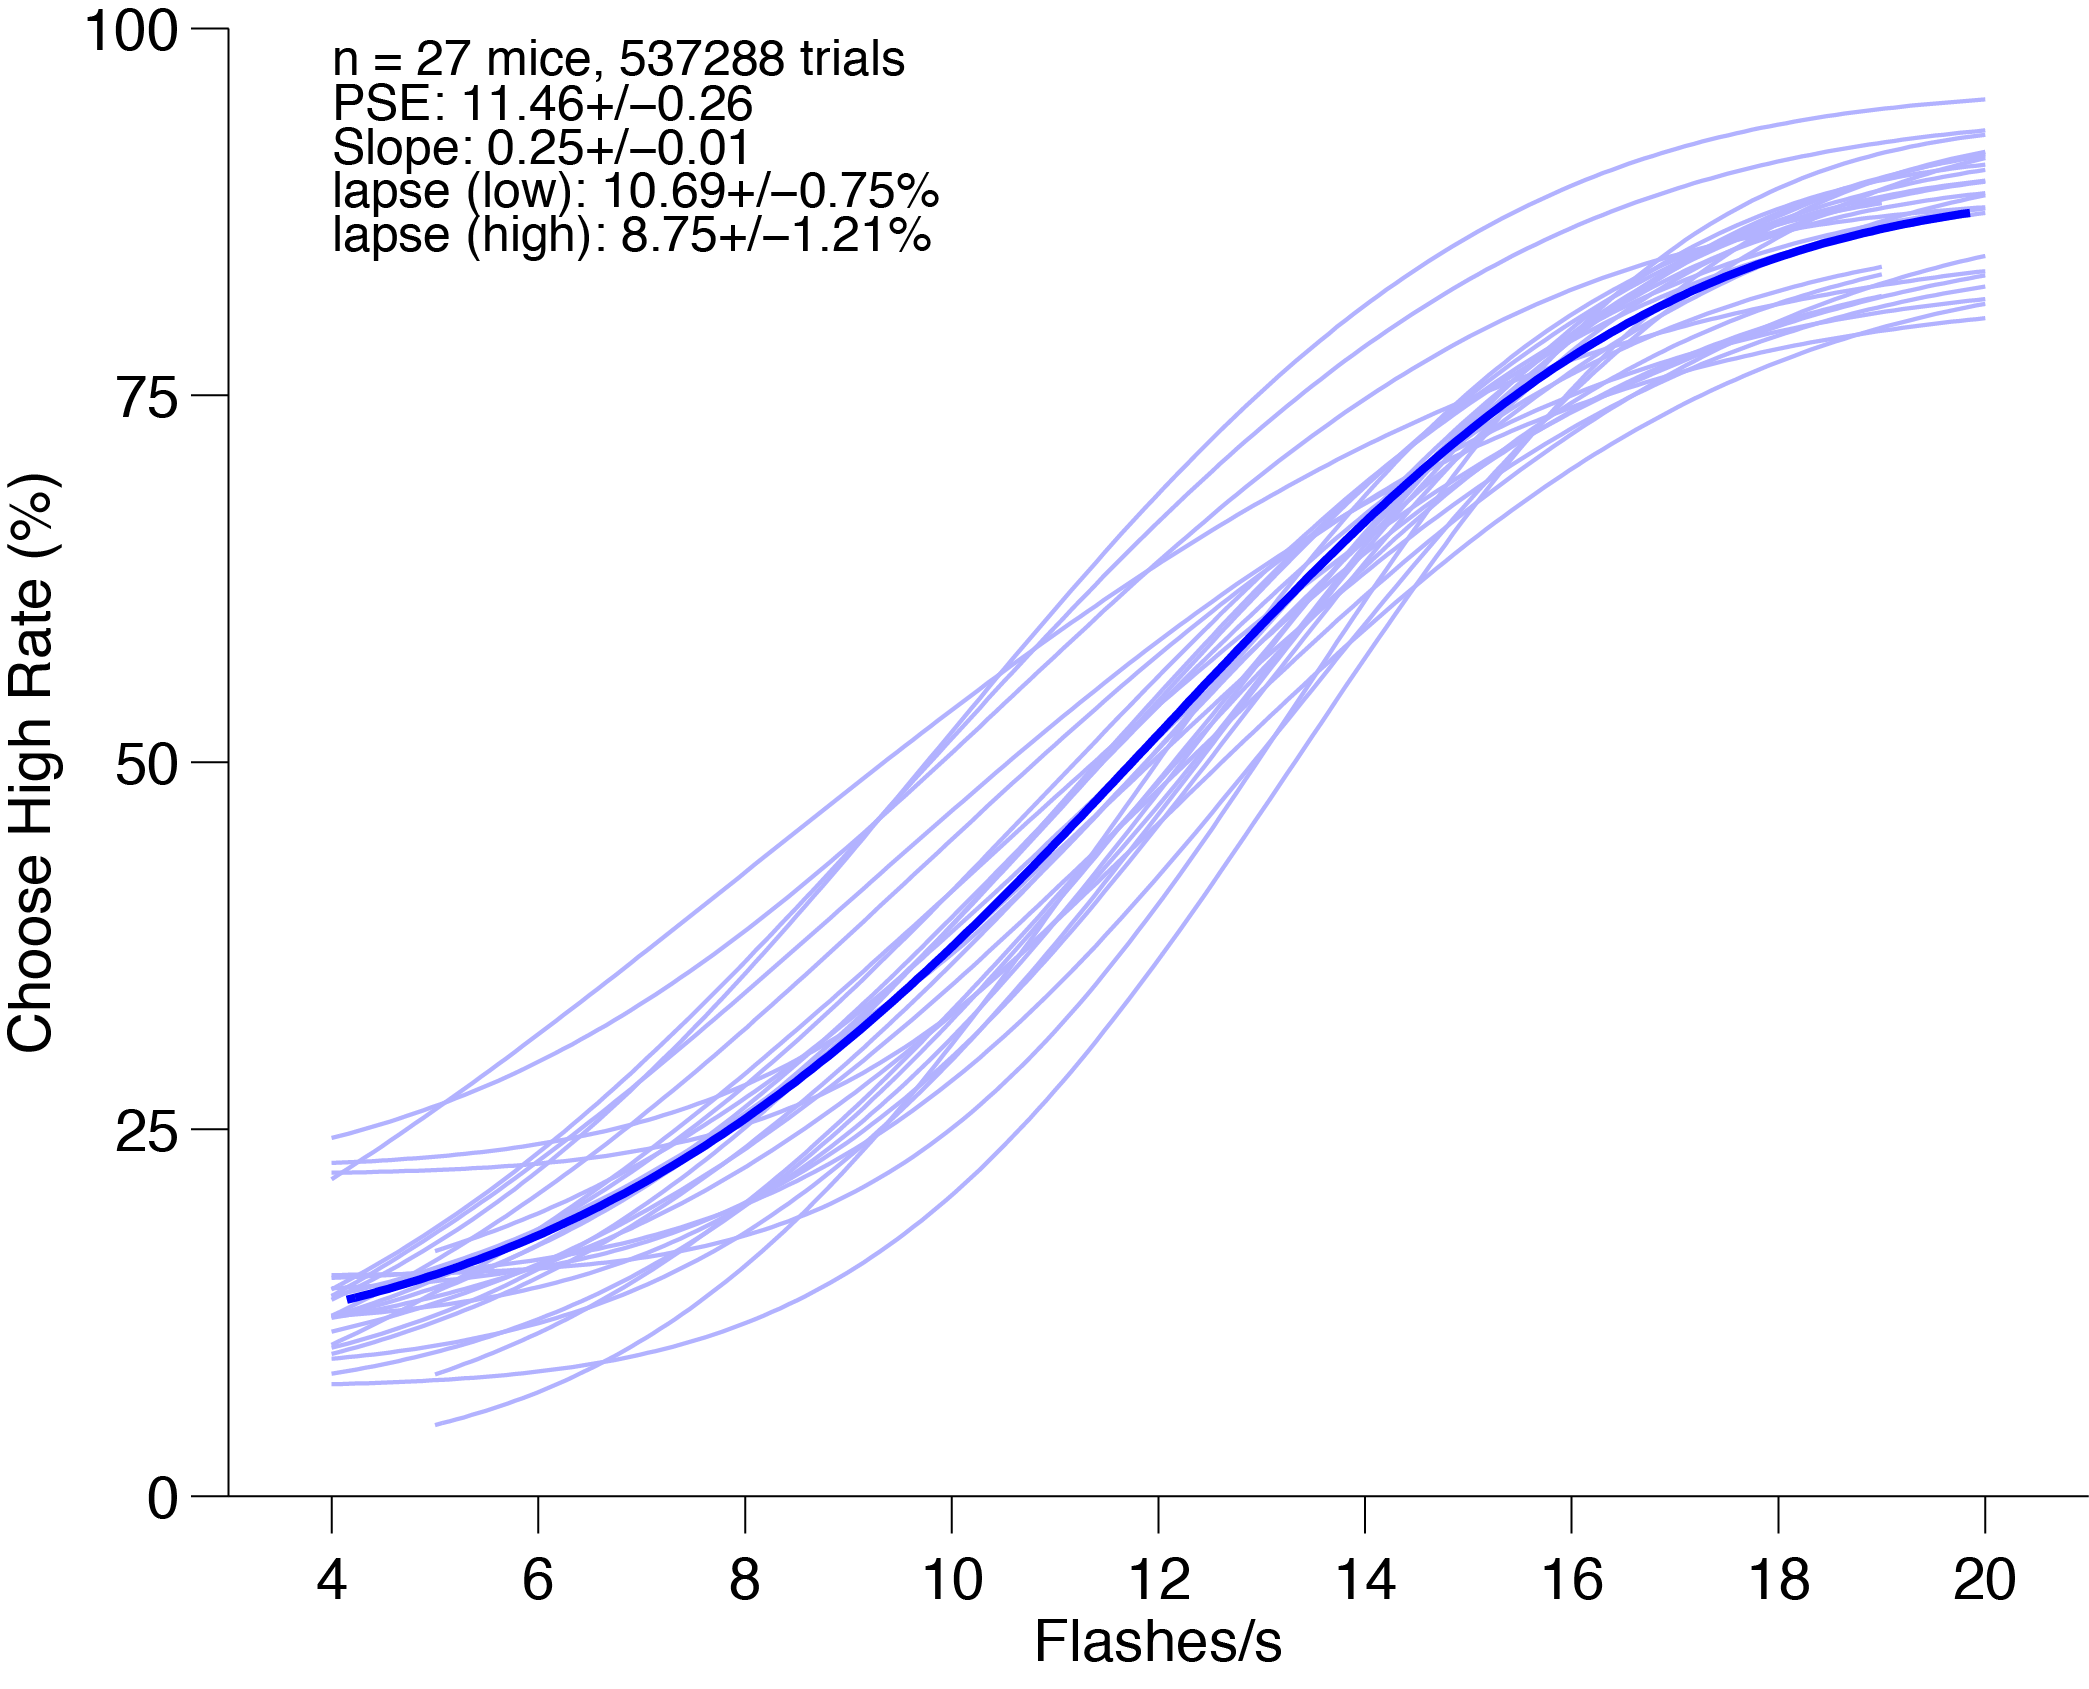
\includegraphics[width=\textwidth]{Figures/chapter2/PMF_pal_27_mice.png}
  \caption[Psychometric Functions]{\textbf{Psychometric Function} fits for individual mice (light blue trace) and average mouse (dark blue). n = 27 mice, across multiple sessions. The psychometric functions were fit with a 4-parameter cumulative Normal distribution to individually fit the intercept, slope, lapse rate and guess rate.}   
   \label{fig:pmfs}
\end{figure}
%----------------------------------------------------------------
\section{Psychophysical Reverse Correlation}
An ideal solution to the task is to sum all the flashes presented during the fixed stimulus presentation period, i.e. apply an equal weight to each incoming flash until the go cue. However, it's not clear whether the mice trained on this task adopted such strategy. For example, the mouse could adopt a strategy where it only pays attention to the first (or second) half of the stimulus. Attention to the flash events early in the sequence would reflect an impulsive strategy, whereas attention to flash events later in the sequence would reflect a leaky or forgetful strategy.\par 
Psychophysical reverse correlation analysis, also known as choice-triggered average, is used to measure the psychophysical kernel of the mice trained on the visual pulses task. There are a number of published methods for performing psychophysical reverse correlation analysis \parencite{Huk2005,Nienborg2007,Raposo2012a,Brunton2013,Katz2016}; however, a simple approach is to use logistic regression  \parencite{Huk2005,Znamenskiy2013,Katz2016}. In the logistic regression approach, the design matrix (i.e. regressors) consists of the pulsatile stimulus sequence for each trial, with 1's to indicate whether a flash occurred in a time bin. The goal is to estimate the weights (coefficients) associated with each time bin.\par 

The logistic regression function for estimating the weights associated with each moment of the stimulus can be written as:
\begin{equation}
	\centering
	\ln(\frac{p_h}{1-p_h}) = \beta_0 + \sum_{i=1}^{N=25} \beta_iI
\end{equation}
where $p_h$ is the probability of choosing the high-rate port, $\emph{I}$ is an indicator variable for whether or not a flash pulse occurred in time bin $\emph{i}$, and $\emph{N}$ is the number of time bins. The coefficients $\beta_0$,...,$\beta_N$ are estimated with the MATLAB function $\emph{glmfit}$. \par 
The logistic reverse correlation approach reveals how each incoming flash, on average, influences the subject's choice. Across mice (Figure \ref{fig:allkernels}), the entire sequence of flashes was informative, as indicated by non-zero regression weights. Also, flashes presented earlier in the sequence appeared to be more informative of the choice than later flashes, on average. The mice appear to make snap judgments about the stimulus sequence, reflecting an impulsive integration strategy. Although the shape of the psychophysical kernel observed in the mice are similar to those observed in nonhuman primate subjects \parencite{Katz2016}, they differ from kernels that have been observed in rats (Figure \ref{fig:ratkernel}) \parencite{Raposo2012,Brunton2013,Scott2015SourcesRats}. In rats, the psychophysical kernels are mostly flat, reflecting an average integration in which evidence is integrated uniformly over time. 
\begin{figure}
  \centering
  	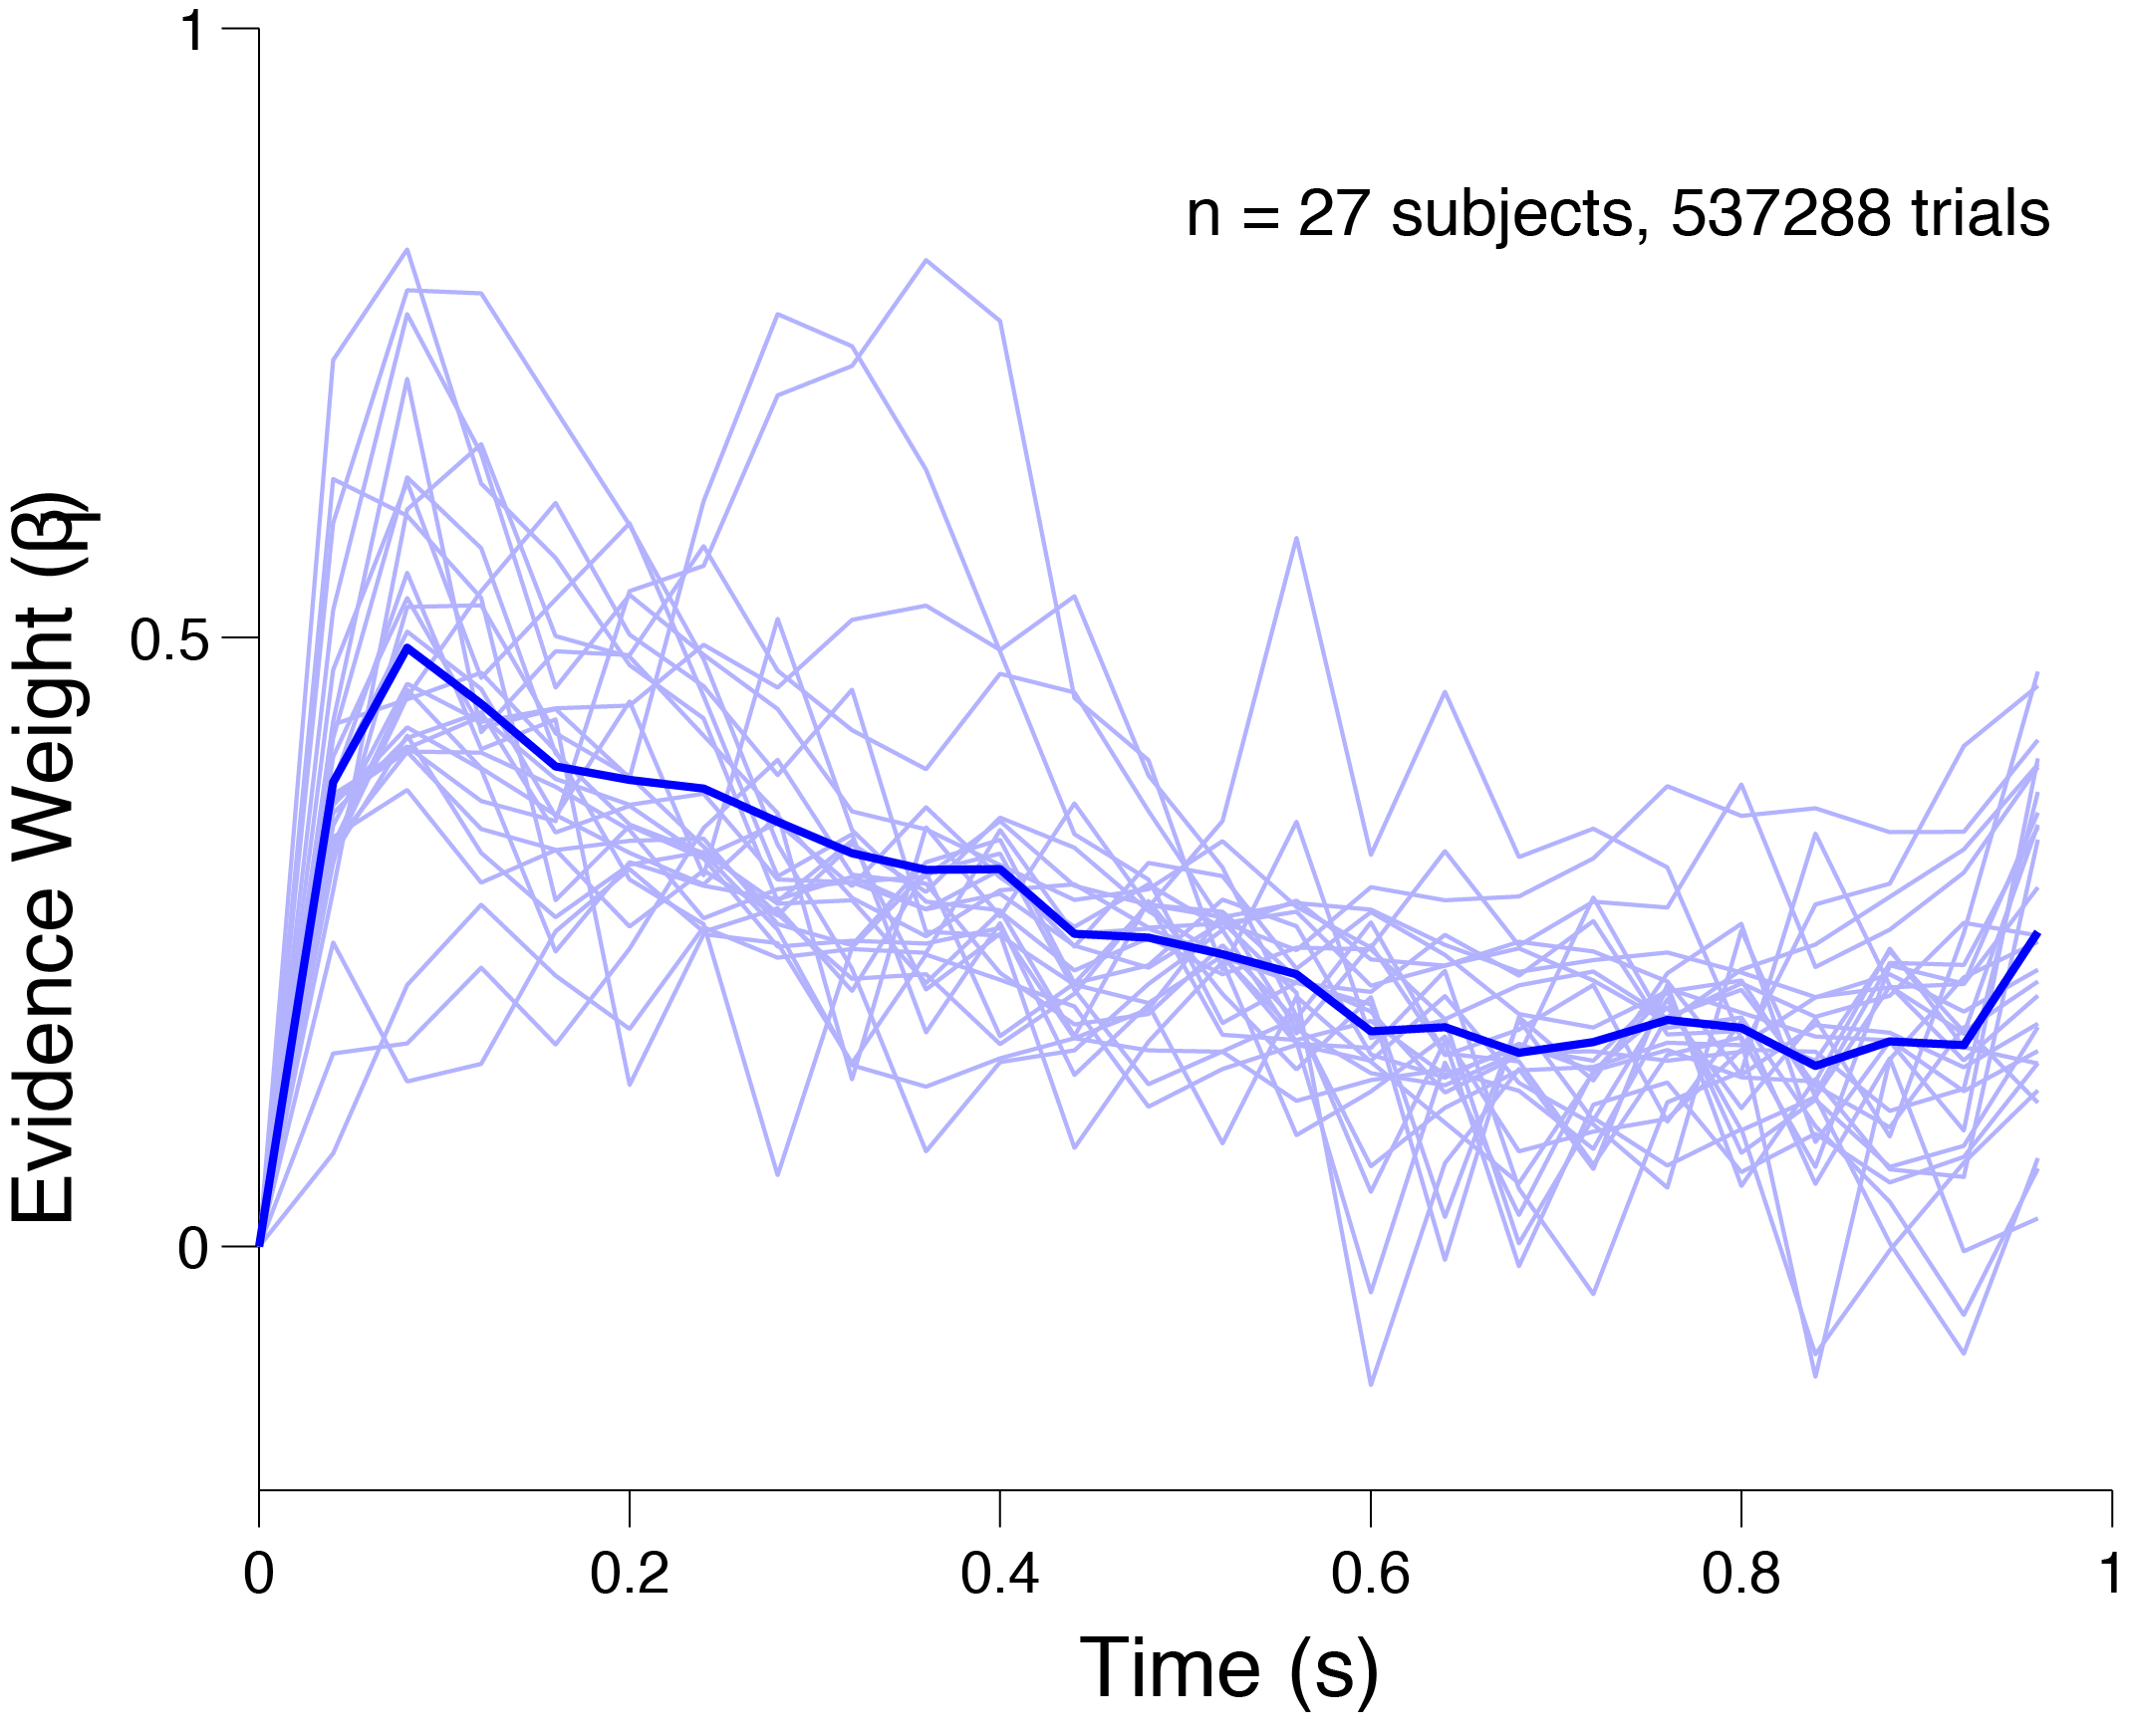
\includegraphics[width=\textwidth]{Figures/chapter2/psychKernel_all_mice.png}
  \caption[Psychophysical Kernels ]{\textbf{Psychophysical Kernels} of individual mice (light blue) and average across mice (dark blue).}
   \label{fig:allkernels}
\end{figure}
%----------------------------------------------------------------------------
\section{Brightness Manipulation}
An alternate strategy to solve the visual pulses task is to accumulate photons or brightness over time, such that the decision is based on the final brightness value. This is a valid strategy given that the flash event rate is directly proportionally to the amount of time the LED is on, and therefore the number of photons emitted (or perceived brightness) over time (Figure \ref{fig:brightness_sim_man}). To test whether subjects performing the visual pulses task were sensitive to changes in brightness, I performed two brightness manipulation experiments. In the first manipulation experiment, the flash sequence was made dimmer or brighter randomly on 5\% of trials. The prediction is that subjects using a brightness strategy will tend to report more high-rate choices on trials with brighter pulse sequences, and on dimmer trials report low-rate choices. For comparison, I also tested rats on the same manipulation. Both mice and rats exhibited shifts in the psychometric function consistent with the predictions (Figure \ref{fig:brightness_exp1}). For mice, changes in brightness had a modest effect on the psychometric performance whereas rats were more sensitive to the  brightness perturbation than mice. \par 
A second, more strict, brightness manipulation was to remove the correlation brightness and the flash rate. To do so, the overall brightness of the flash sequence was made proportional to the flash event rate, such that the total brightness over time was the same across flash rates  (Figure \ref{fig:brightness_sim_man}). If the subjects were indeed invariant to the total brightness over time, and instead were counting, this manipulation should not interfere with their performance. However, when the scaled brightness was introduced randomly on 5\% of trials, the performance of both mice and rats were severely affected. \par 
The brightness manipulations revealed that the subjects were not invariant to the brightness. The manipulations do not suggest that the subjects are incapable of using a counting strategy to solve the visual pulses categorization task, especially in the case of the mice. Rather, these experiments reveal that the use of brightness is a valid alternate (or parallel) strategy given that the correlation between the total LED ON time is and the total number of flashes exists in the stimulus (Figure \ref{fig:brightness_sim}). The decreased performance on the second brightness manipulation trials could be explained by the fact that the stimulus is very different from the one on which the subjects were trained. Future efforts could explore whether rodents can be trained on a stimulus similar to Figure \ref{fig:brightness_sim_man}, without the brightness correlation. 

\begin{figure}
  \centering
  	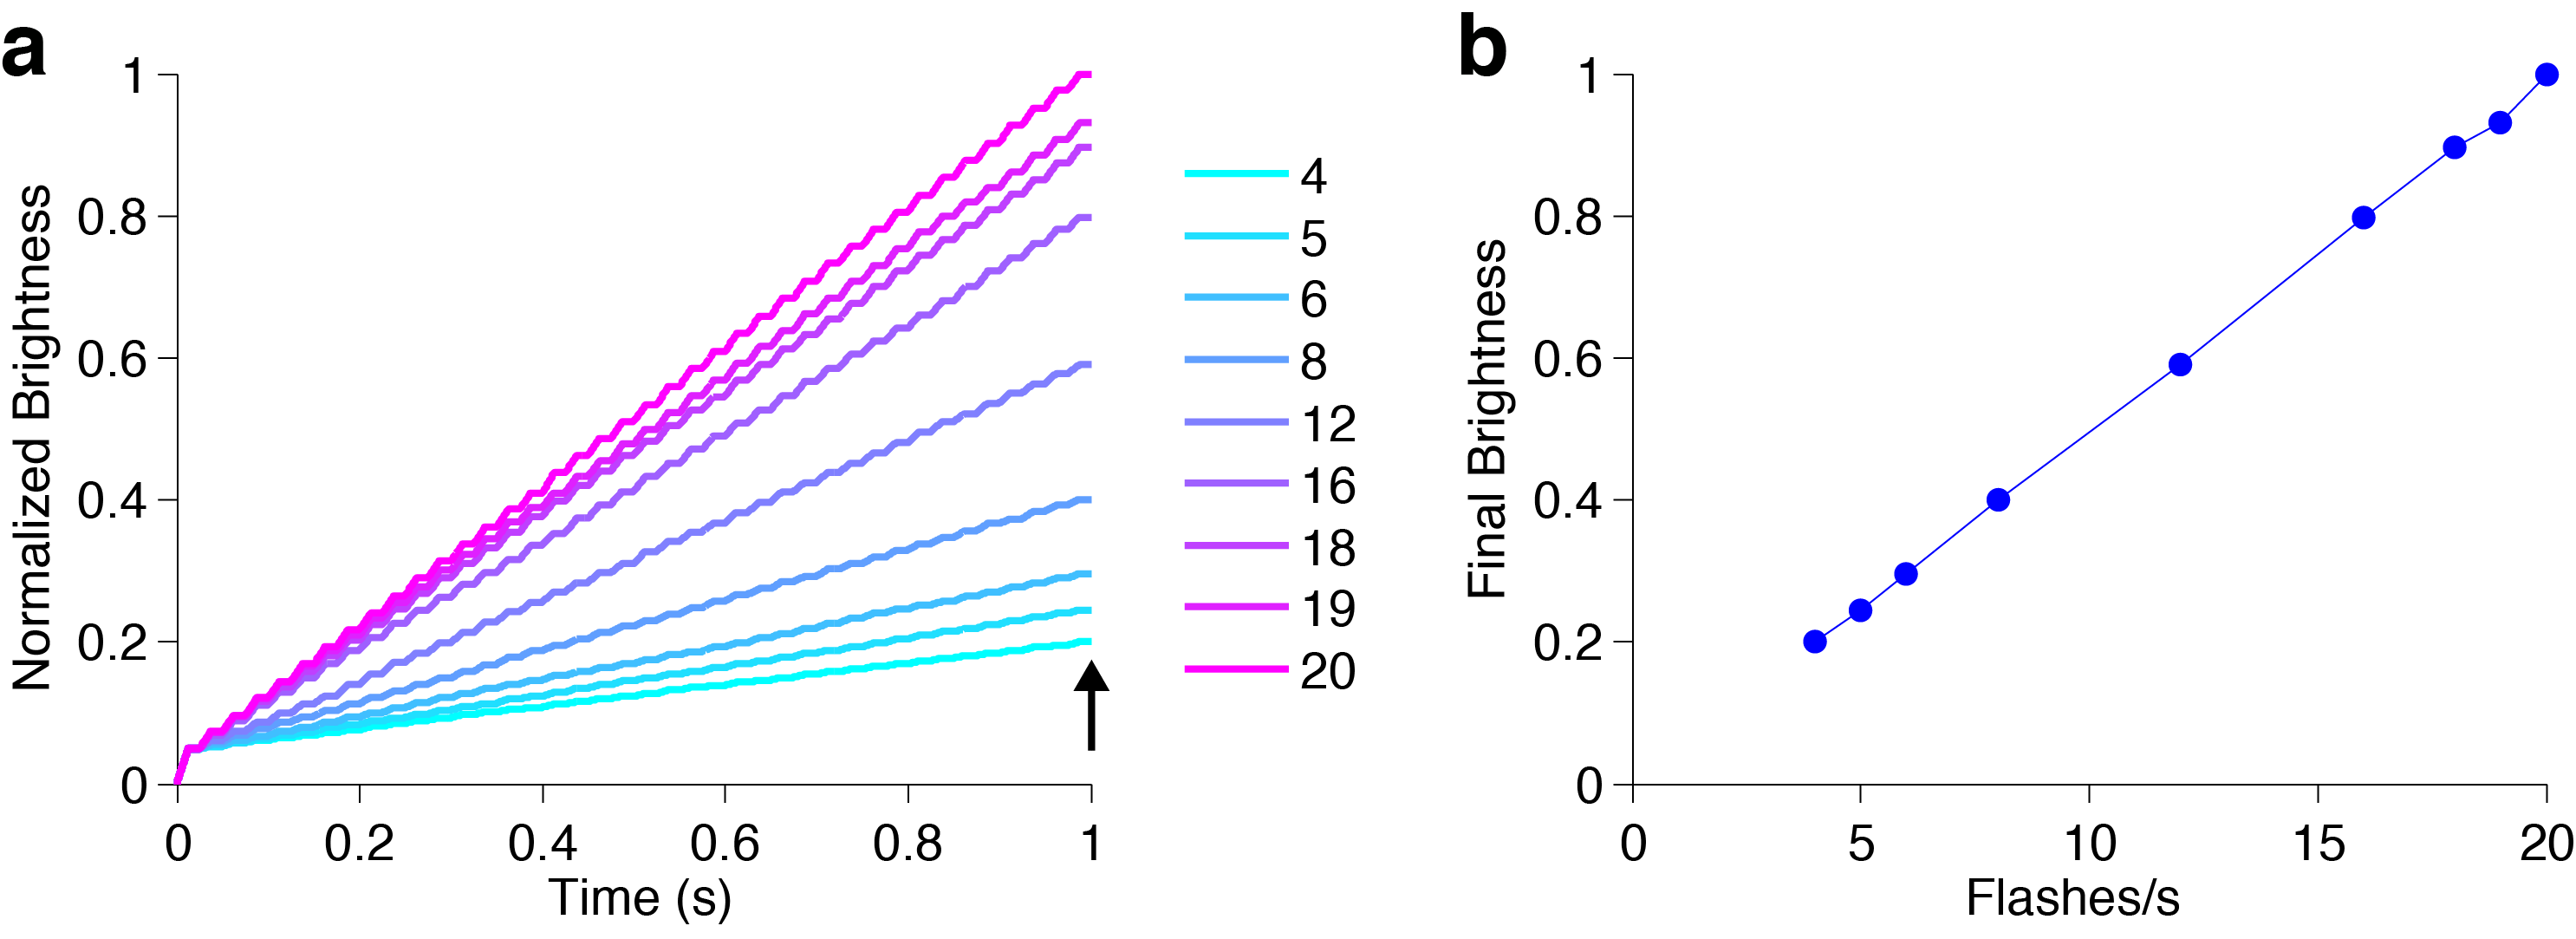
\includegraphics[width=\textwidth]{Figures/chapter2/brightness_simulation_unscaled.png}
  \caption[Flash Rate is Correlated with Brightness Over Time]{\textbf{Trial Flash Rate is Correlated with Brightness Over Time}. (a) Schematic of simulated average brightness (normalized) across time for individual flash rates. Simulated brightness curves computed as the cumulative sum of the flash sequence for a given flash rate. (b) Final simulated brightness value (at arrow in (a)) plotted against flash rate.}
   \label{fig:brightness_sim}
\end{figure}

\begin{figure}
  \centering
  	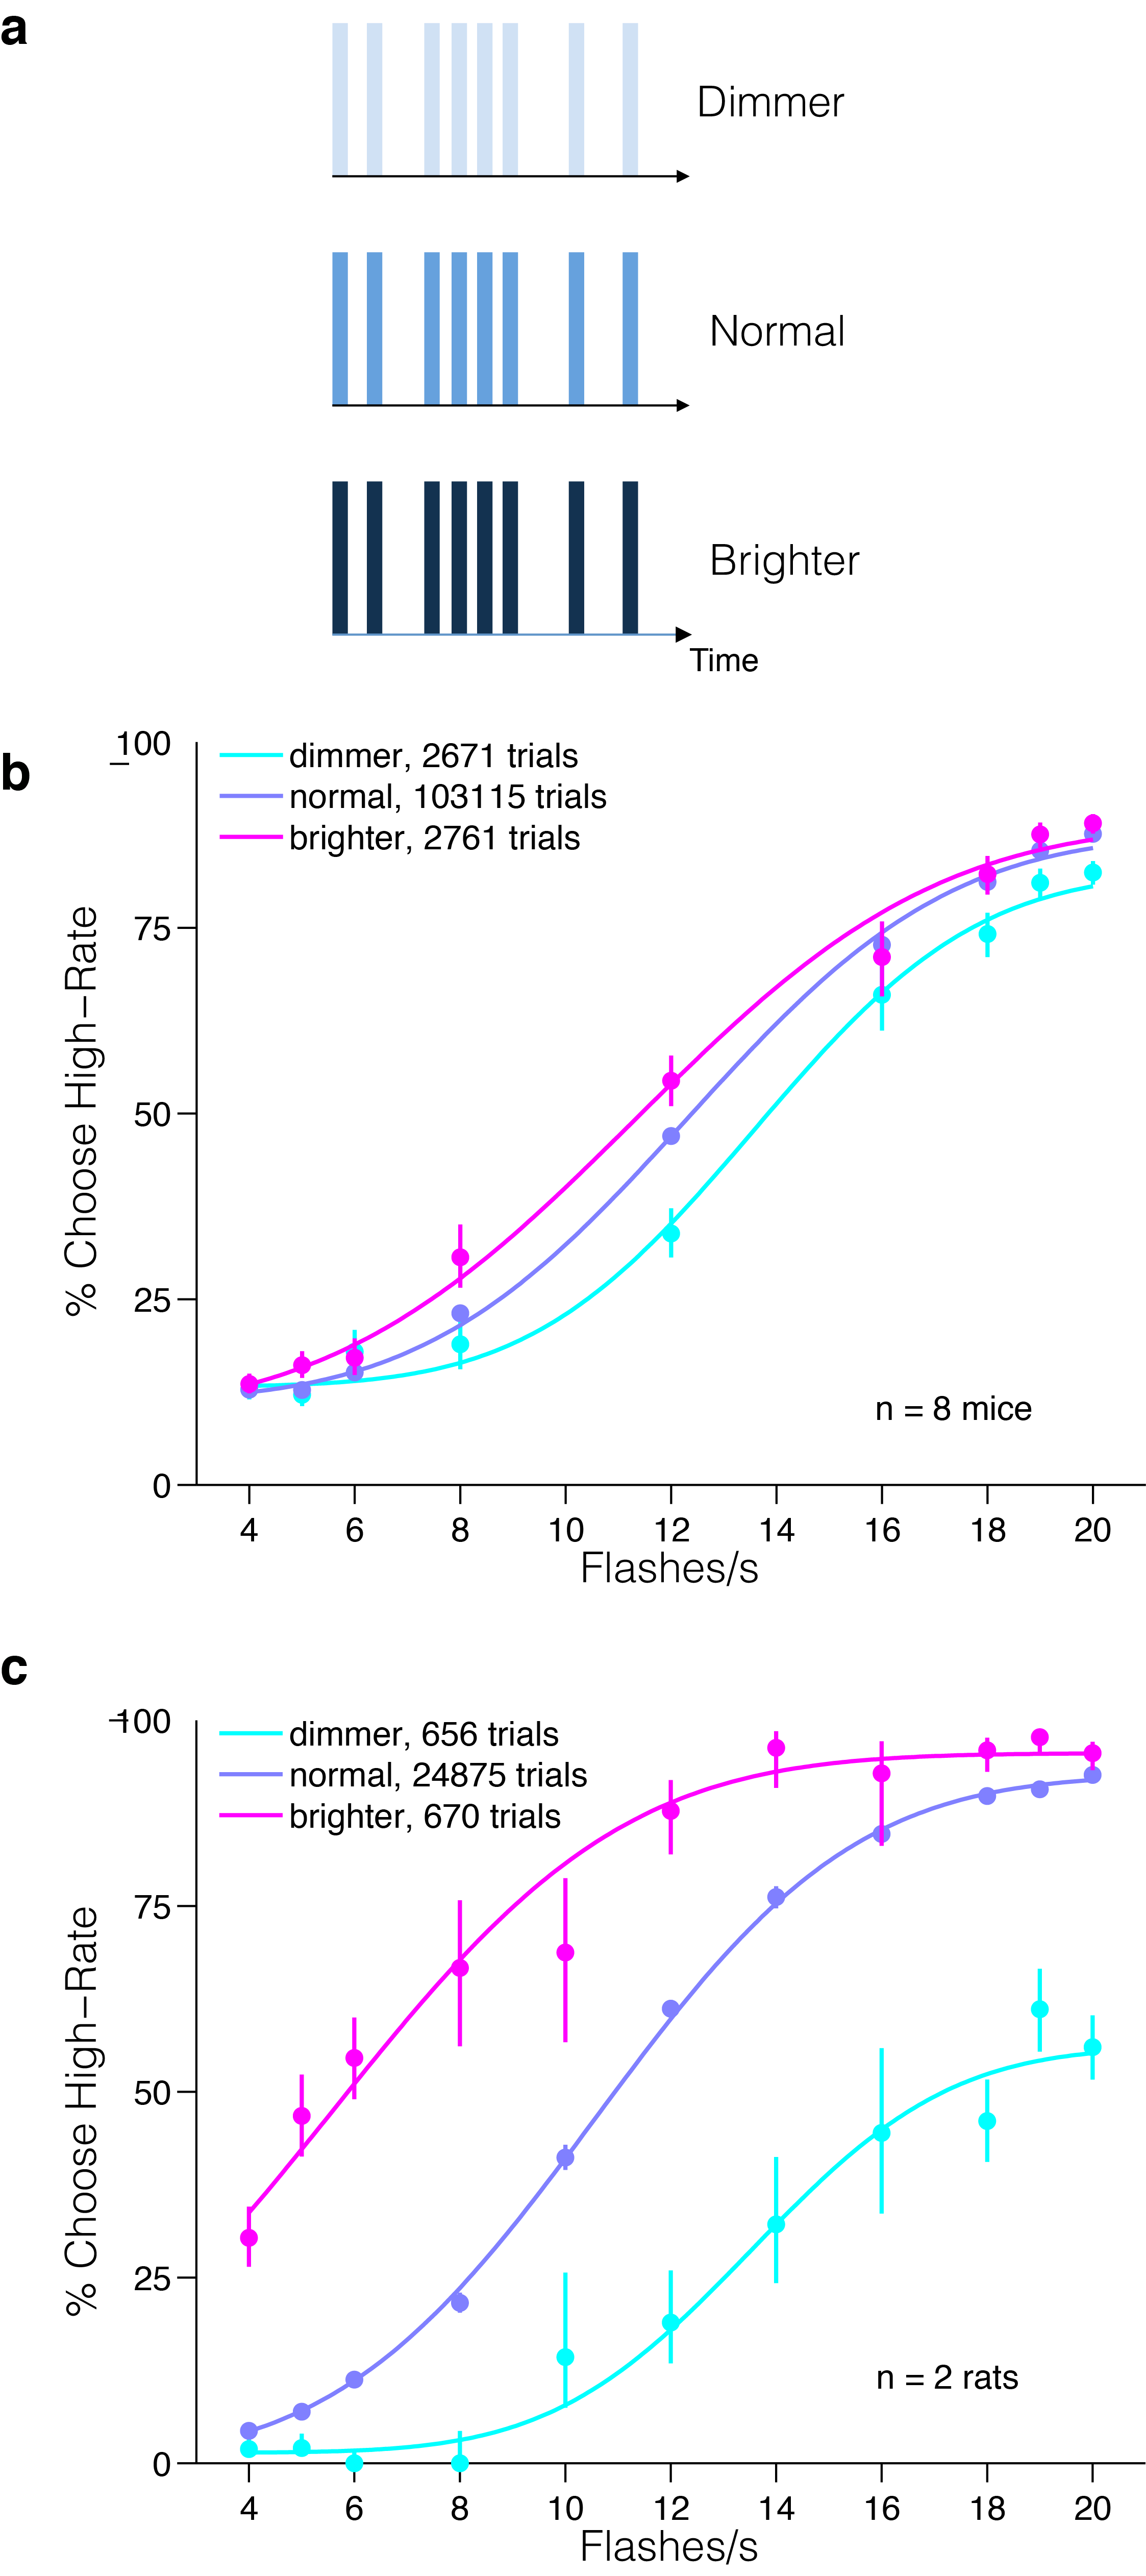
\includegraphics[width=\textwidth,height=0.8\textheight,keepaspectratio]{Figures/chapter2/brightness_manipulation_1.png}
  \caption[Brightness Manipulation Experiment 1]{\textbf{Brightness Manipulation Experiment 1}. (a) Schematic of random pulses sequence (8 flashes/s). The density of individual flashes were varied such that the flashes appeared dimmer or brighter than normal.(b) Mice (n = 8) or (c) rats (n=2) were presented with brighter (magenta) or dimmer (cyan) pulse sequences randomly on 5\% of trials. Circles represent subjects' behavioral response. Solid line represents 4-parameter cumulative Gaussian psychometric function fit to the data. Error bars represent Wilson binomial (95\%) confidence intervals.}
   \label{fig:brightness_exp1}
\end{figure}

\begin{figure}
  \centering
  	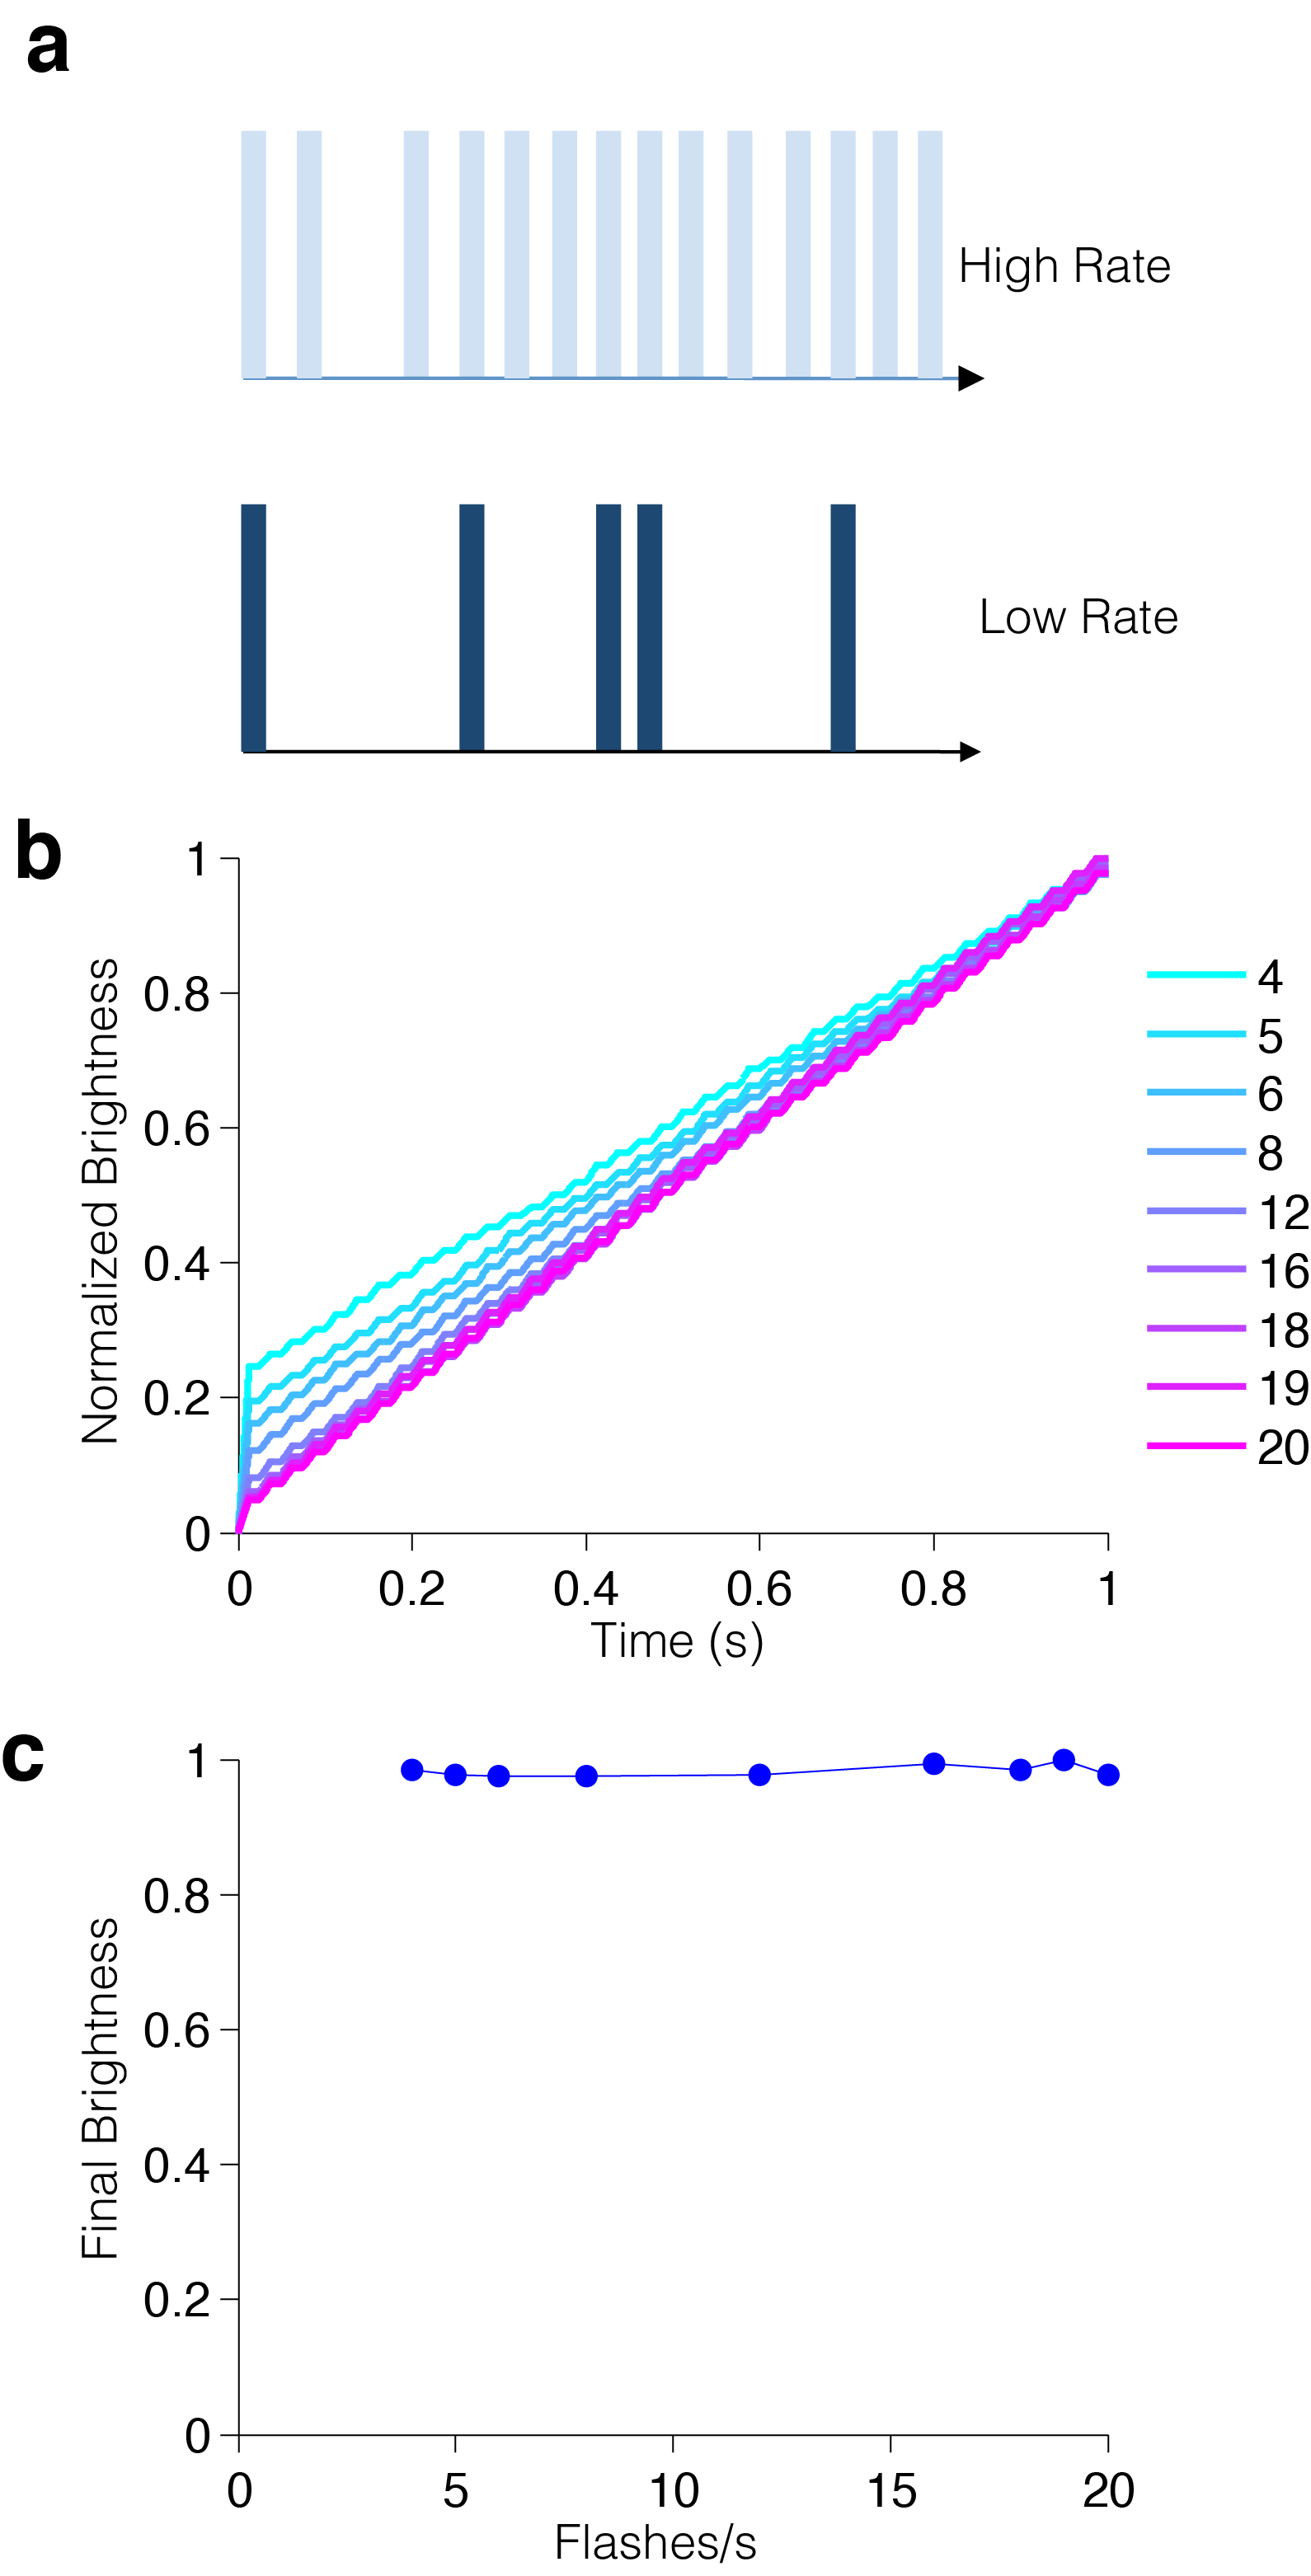
\includegraphics[width=\textwidth,height=0.8\textheight,keepaspectratio]{Figures/chapter2/brightness_simulation_scaled.png}
  \caption[Brightness Manipulation Experiment 2 Schematic]{\textbf{Brightness Manipulation Experiment 2 Schematic}. (a) Schematic of random pulses sequence for high-rate and low-rate example. The density of individual flashes are scaled inversely with the flash rate, such that the low-rate sequences are more dense than high-rate sequences. (b) Brightness over time is overlap for individual flash rate and (c) the final brightness value is equivalent across flash rates. }
   \label{fig:brightness_sim_man}
\end{figure}

\begin{figure}
  \centering
  	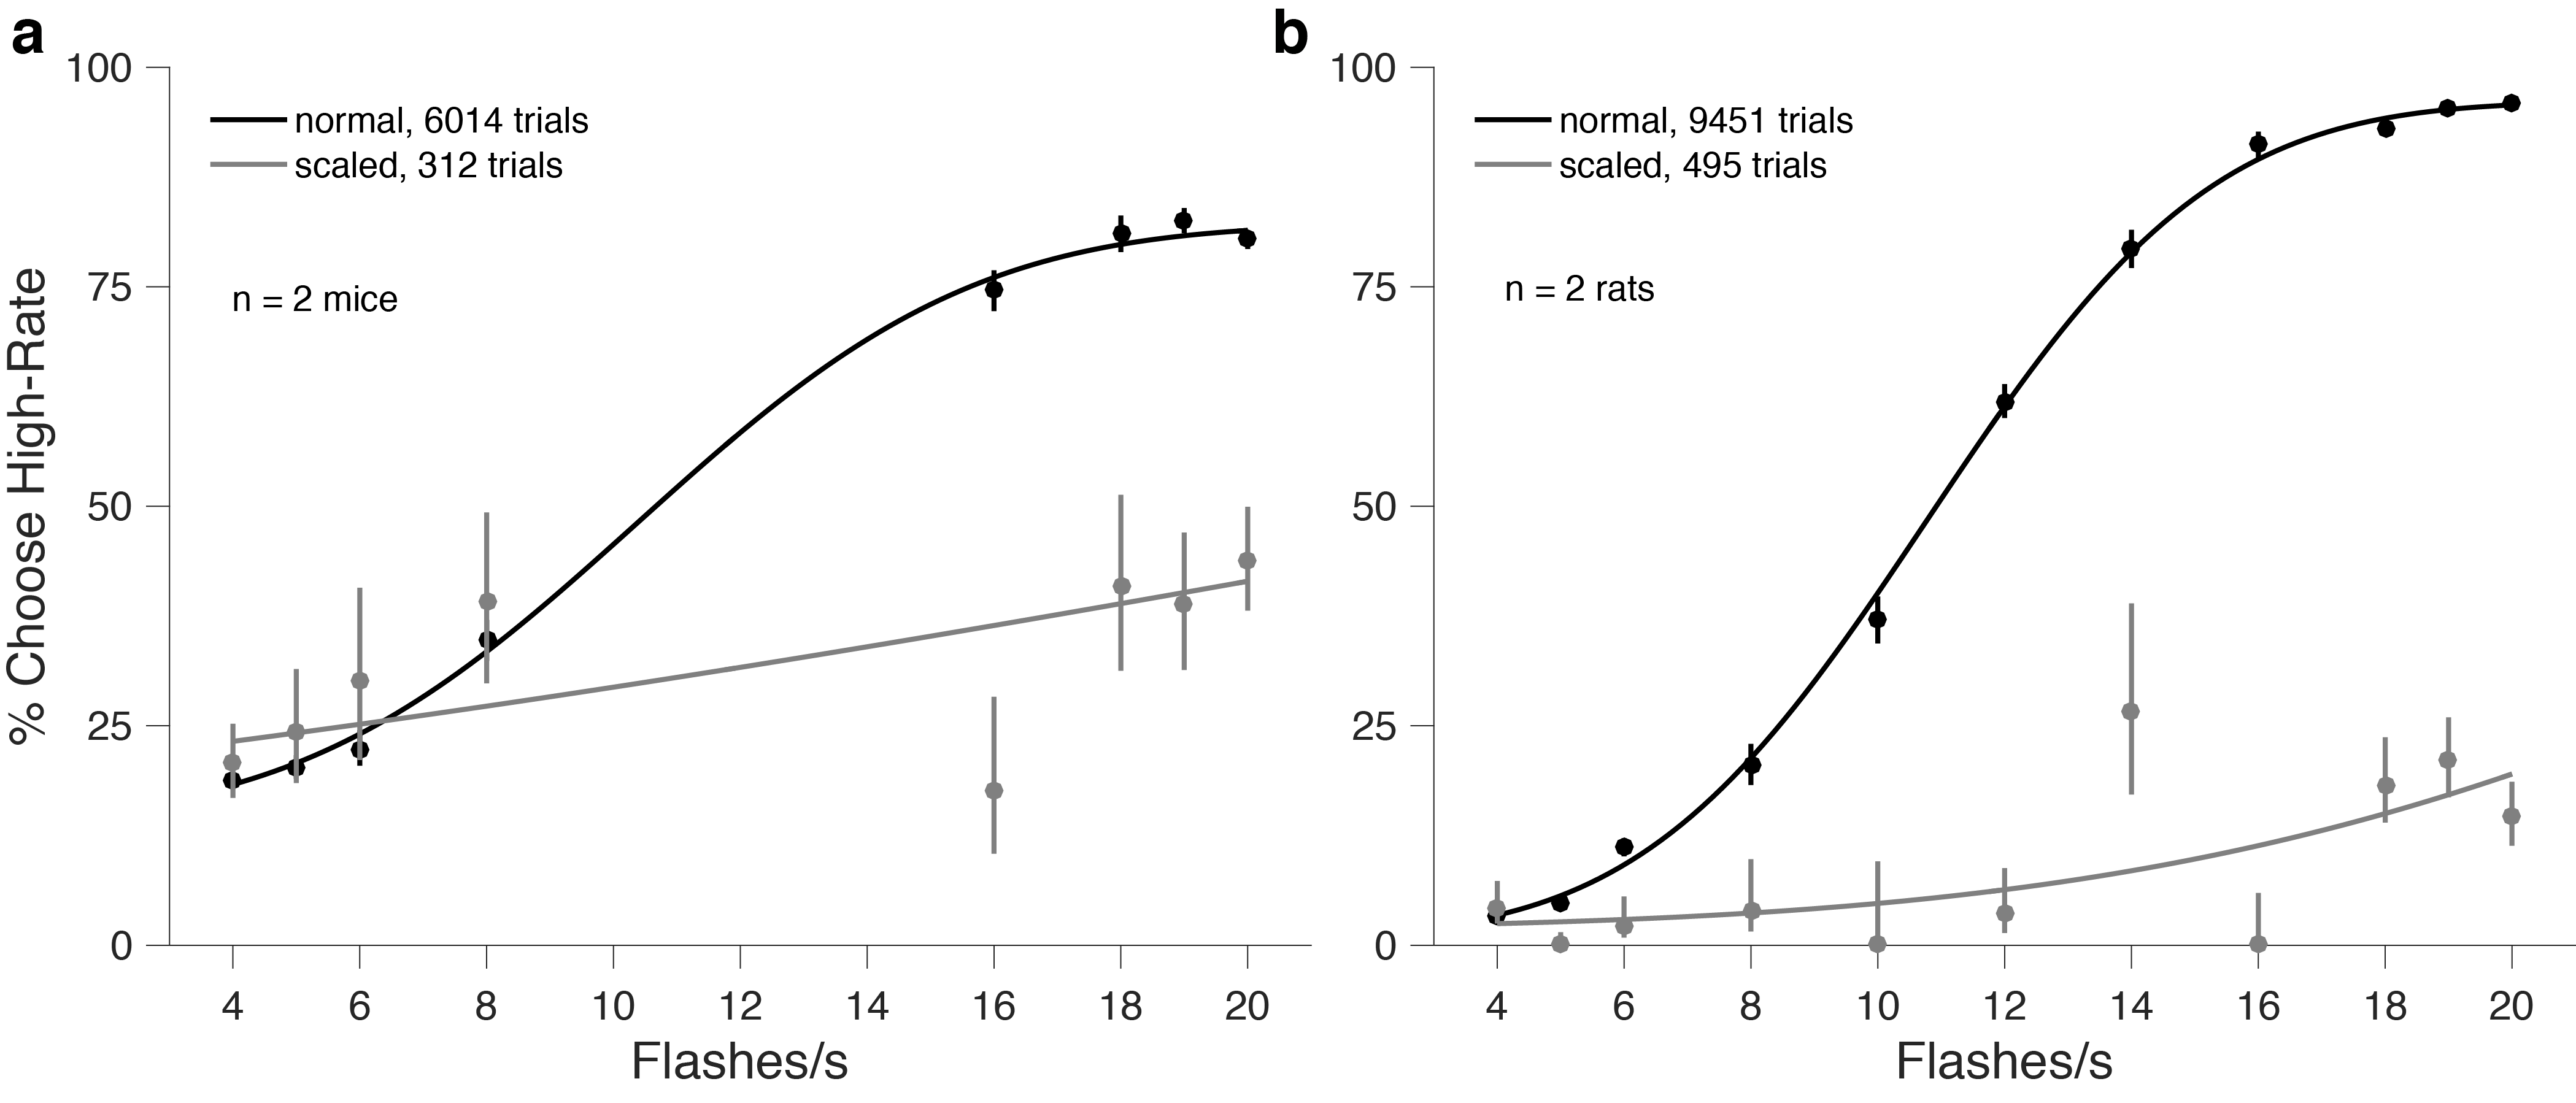
\includegraphics[width=\textwidth]{Figures/chapter2/brightness_manipulation_2.png}
  \caption[Brightness Manipulation Experiment 2]{\textbf{Brightness Manipulation Experiment 2}. (a) Mice or (b) rats were presented with the brightness scaled  pulse sequence randomly on 5\% of trials (open circle, gray curve). Circles represent subjects' behavioral response. Solid line represents 4-parameter cumulative Gaussian psychometric function fit to the data. Error bars represent Wilson binomial (95\%) confidence intervals. }
   \label{fig:brightness_exp2}
\end{figure}
%--------------------------------------------------------------------
\section{Previous Choice History Influence}
Several studies have found that both human and animal subjects performing perceptual tasks are influenced by previous choices \parencite{Busse2011,Frund2014,Scott2015SourcesRats,Abrahamyan2016,Urai2017}, even though the trials are independent and presented randomly. We used two quantitative models to assess whether mice trained to make categorical decisions about visual pulsatile stimuli were susceptible to choices made on previous trials.\par 
The first approach, assessed whether success or failure on the most recent trial influenced the performance on the current trial \parencite{Busse2011}: 
\begin{equation}
	\centering
	\ln(\frac{p_h}{1-p_h}) = \beta_0 + \beta_E E(t) + \beta_S I_{success} (t-1) + \beta_F I_{failure} (t-1)
    \label{eq:BusseChoice}
\end{equation}
where \emph{t} indicates the current trial and $\emph{E}$ is the signed stimulus evidence of the current trial. Evidence is computed as the difference between the flash rate of the trial and the category boundary (12 flashes/s). \emph{$I_{success}$} and \emph{$I_{failure}$} are indicator variables for success (reward) and failure on the previous trial, respectively. The coefficients ($\beta_0$,$\beta_E$,$\beta_S$,$\beta_F$) were estimated with MATLAB \emph{glmfit}.\par 
Figure \ref{fig:failsuccesshist} is a scatter plot of the coefficients for previous success, $\beta_S$, and previous failures, $\beta_F$. All mice (n = 27) had positive $\beta_S$ coefficients, indicating that mice tended to repeat the same choice on the current trial if they had been rewarded on the previous trial. Nearly half the group of mice had positive $\beta_F$ coefficients, meaning that these mice tended to repeat failures (Figure \ref{fig:failsuccesshist} , Stay quadrant). The remaining mice with negative $\beta_F$ coefficients had a tendency to switch choices if they were unsuccessful on the previous trials Figure \ref{fig:failsuccesshist}, (Win-Stay, Lose Switch quadrant). The observed trial history patterns are similar to those of human subjects performing a perceptual decision making task \parencite{Abrahamyan2016}. \par 
\begin{figure}
  \centering
  	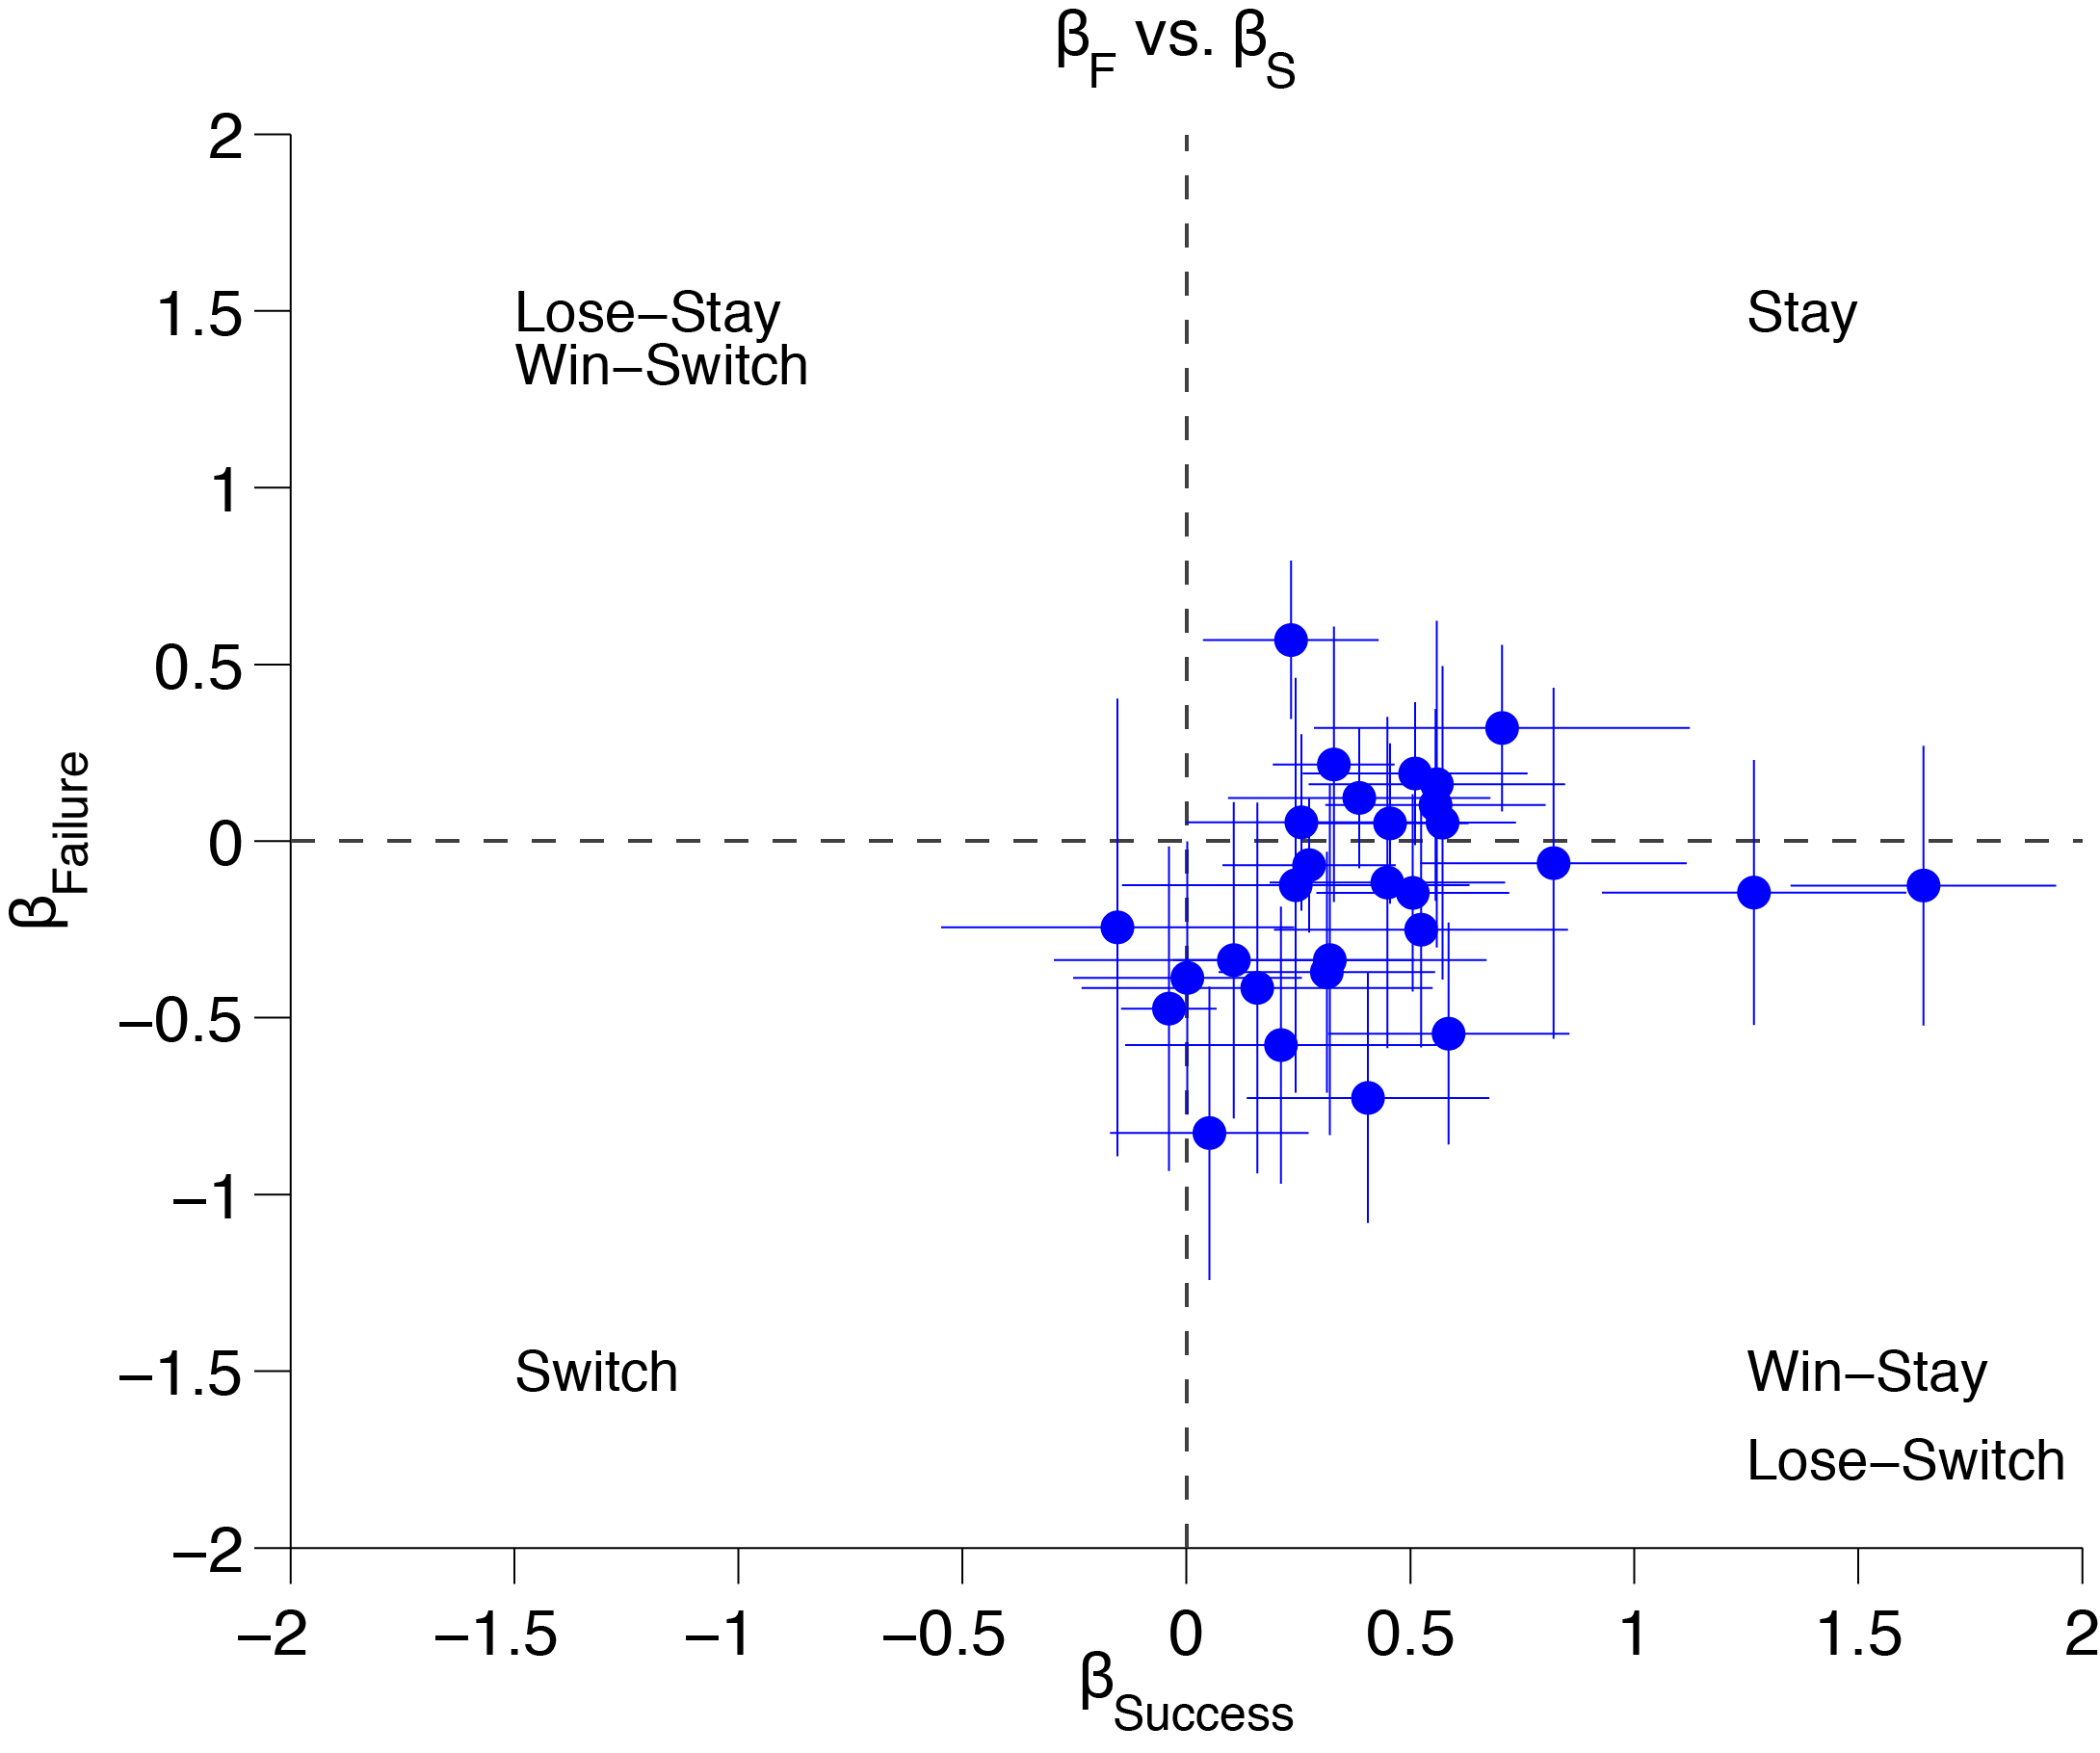
\includegraphics[width=\textwidth]{Figures/chapter2/history_failure_success_model_error_bars.png}
  \caption[Previous Choice History - Success and Failure]{\textbf{Previous Choice History - Success and Failure} Influence on the current trial for each mouse (n = 27 mice). Coefficients estimated for each session individually. Mean coefficients are plotted. Error bars represent standard error of the mean.}
   \label{fig:failsuccesshist}
\end{figure}
A second approach is to assess the influence of the history of previous choices on the current choice. The probabilistic model is an extension of Equation \ref{eq:BusseChoice} and equivalent to the model described in \textcite{Frund2014}:
\begin{equation}
	\centering
	\ln(\frac{p_h}{1-p_h}) = \beta_0 + \beta_E E(t) + \sum_{\tau = 1}^{T=7} \beta_{E(\tau)} E_\tau + \beta_{C(\tau)} C_\tau
\end{equation}
where \emph{t} indicates the current trial and  $\emph{E}$ is the signed stimulus evidence of the current trial. The additional regressors $E_\tau$ and $C_\tau$ represent the evidence and choice on $\tau$ previous trials in the past, respectively. Again, the coefficients ($\beta_0$,$\beta_E$,$\beta_{E(\tau)}$, and $\beta_{C(\tau)}$) were estimated with MATLAB \emph{glmfit}.\par 
\begin{figure}
  \centering
  	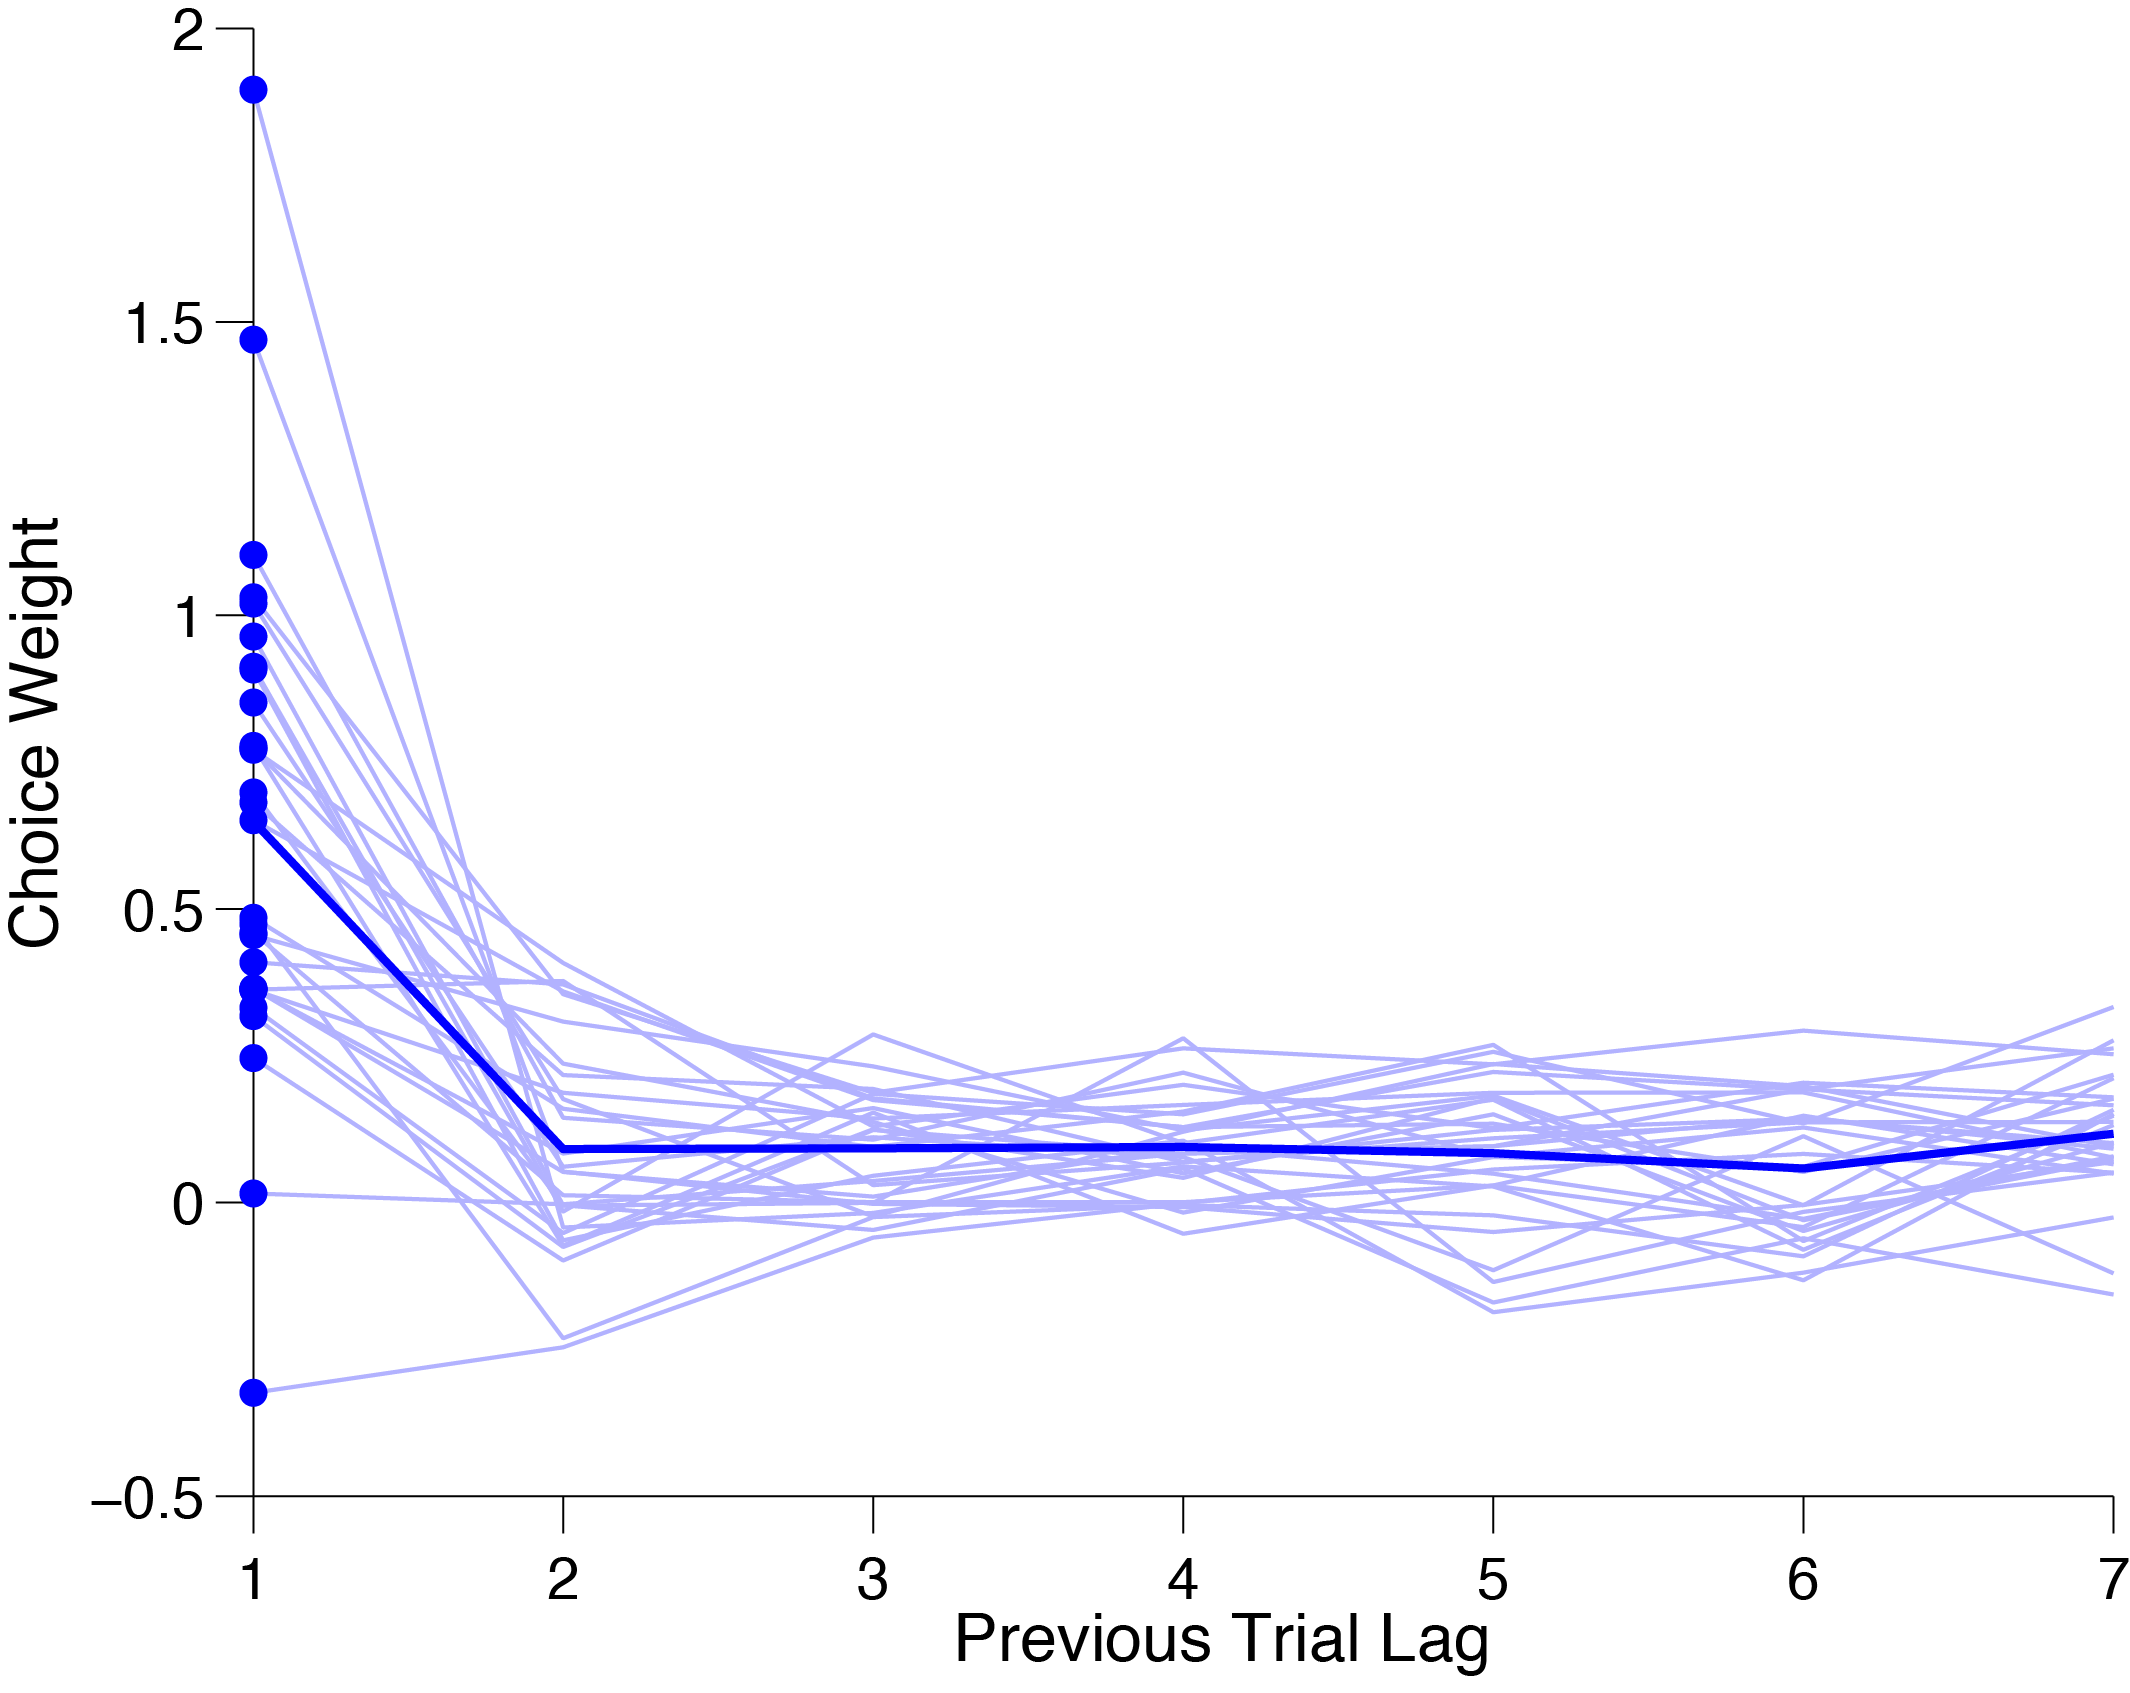
\includegraphics[width=\textwidth]{Figures/chapter2/history_past_choices_model.png}
  \caption[Influence of Previous Choice History]{\textbf{Influence of Previous Choice History} Choice weights, $\beta_{C(\tau)}$, associated with the previous seven trials. Light blue traces represent individual subjects (n = 27), Dark blue trace is the average across subjects.}
   \label{fig:prevchoiceshist}
\end{figure}
The model of the history of previous choices revealed that the most recent choice ($\tau$ = 1) had a greater influence on the choice of the current trial, than all other trials in the past (Figure \ref{fig:prevchoiceshist}). Almost all the subjects exhibited the same trend. 
%----------------------------------------------------------------------------
\section{Behavioral Correlates of Decision Uncertainty}
Response time is inversely correlated with decision certainty (i.e. confidence) \parencite{Kiani2014,Sanders2016,Urai2017}. I evaluated whether the response times of the mice trained on the visual pulses task exhibited the three signatures of decision uncertainty, the complement of the decision confidence \parencite{Kepecs2008,Sanders2016,Urai2017}, which make the following predictions: (1) accuracy monotonically decreases with uncertainty (Figure \ref{fig:uncertainty}a), (2) average uncertainty decreases with evidence strength for correct choices and increases for incorrect choices (Figure \ref{fig:uncertainty}b), and lastly, for fixed evidence strengths, low and high uncertainty change the slope of the psychometric function (Figure \ref{fig:uncertainty}c). \par 
Although the mice were trained to perform the task under fixed duration (or interrogation) protocol \parencite{Bogacz2006}, we measured a proxy of reaction time as the time it takes the mice to exit the center port and enter the side reward port. A similar approach was used in a recent study by \textcite{Urai2017} to correlate response time of human subjects performing a fixed duration perceptual decision-making task.\par 
\begin{figure}
  \centering
  	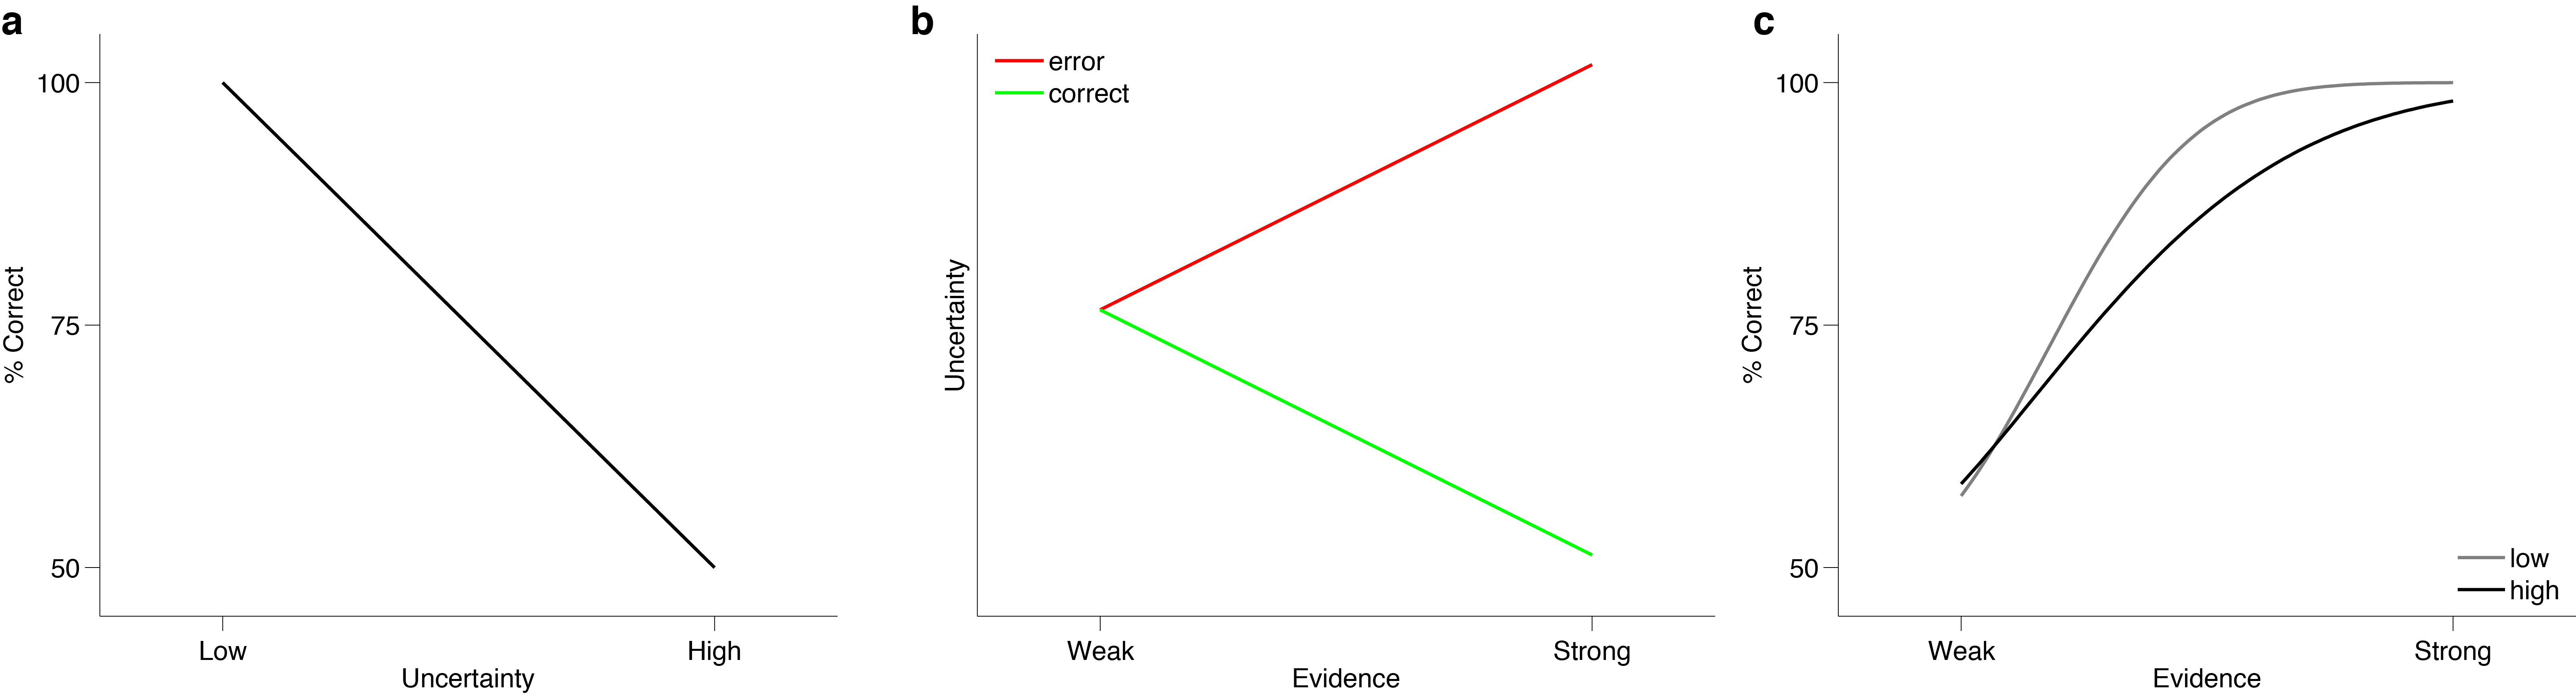
\includegraphics[width=\textwidth]{Figures/chapter2/schematic_uncertainty_predictions.png}
  \caption[Schematic of Signatures of Decision Uncertainty Predictions]{\textbf{Schematic of Decision Uncertainty Predictions} (a) Monotonic decrease in accuracy with uncertainty Scaling of accuracy (b) Scaling of mean uncertainty with evidence strength for correct (green) and incorrect (red) choices (c) Psychometric function predictions for low (gray) and high uncertainty (gray). Adapted from \textcite{Urai2017,Sanders2016}}
   \label{fig:uncertainty}
\end{figure}
For the following analyses we evaluated mice trained under two different conditions. One group of mice (n = 10) were trained with walls between the center port and the side ports and the second group were trained without the walls (n = 19 mice) and rewarded in the center (0.5 $\mu$L) for waiting the minimum required wait duration. The group trained with walls were trained before we implemented the center reward approach (Figure \ref{fig:completeRate}). In the early stages of the thesis project, walls were used to reduce the subjects' impulsive tendencies to break center fixation and respond to the side port. The walls also helped to make the subjects' movements more stereotyped across animals. However, when trained mice were tethered with optical fibers for optogenetic stimulation (or microdrives for neural recordings), the walls obstructed the subjects' movements, so we removed the walls entirely from the training protocol.\par 
\begin{figure}
  \centering
  	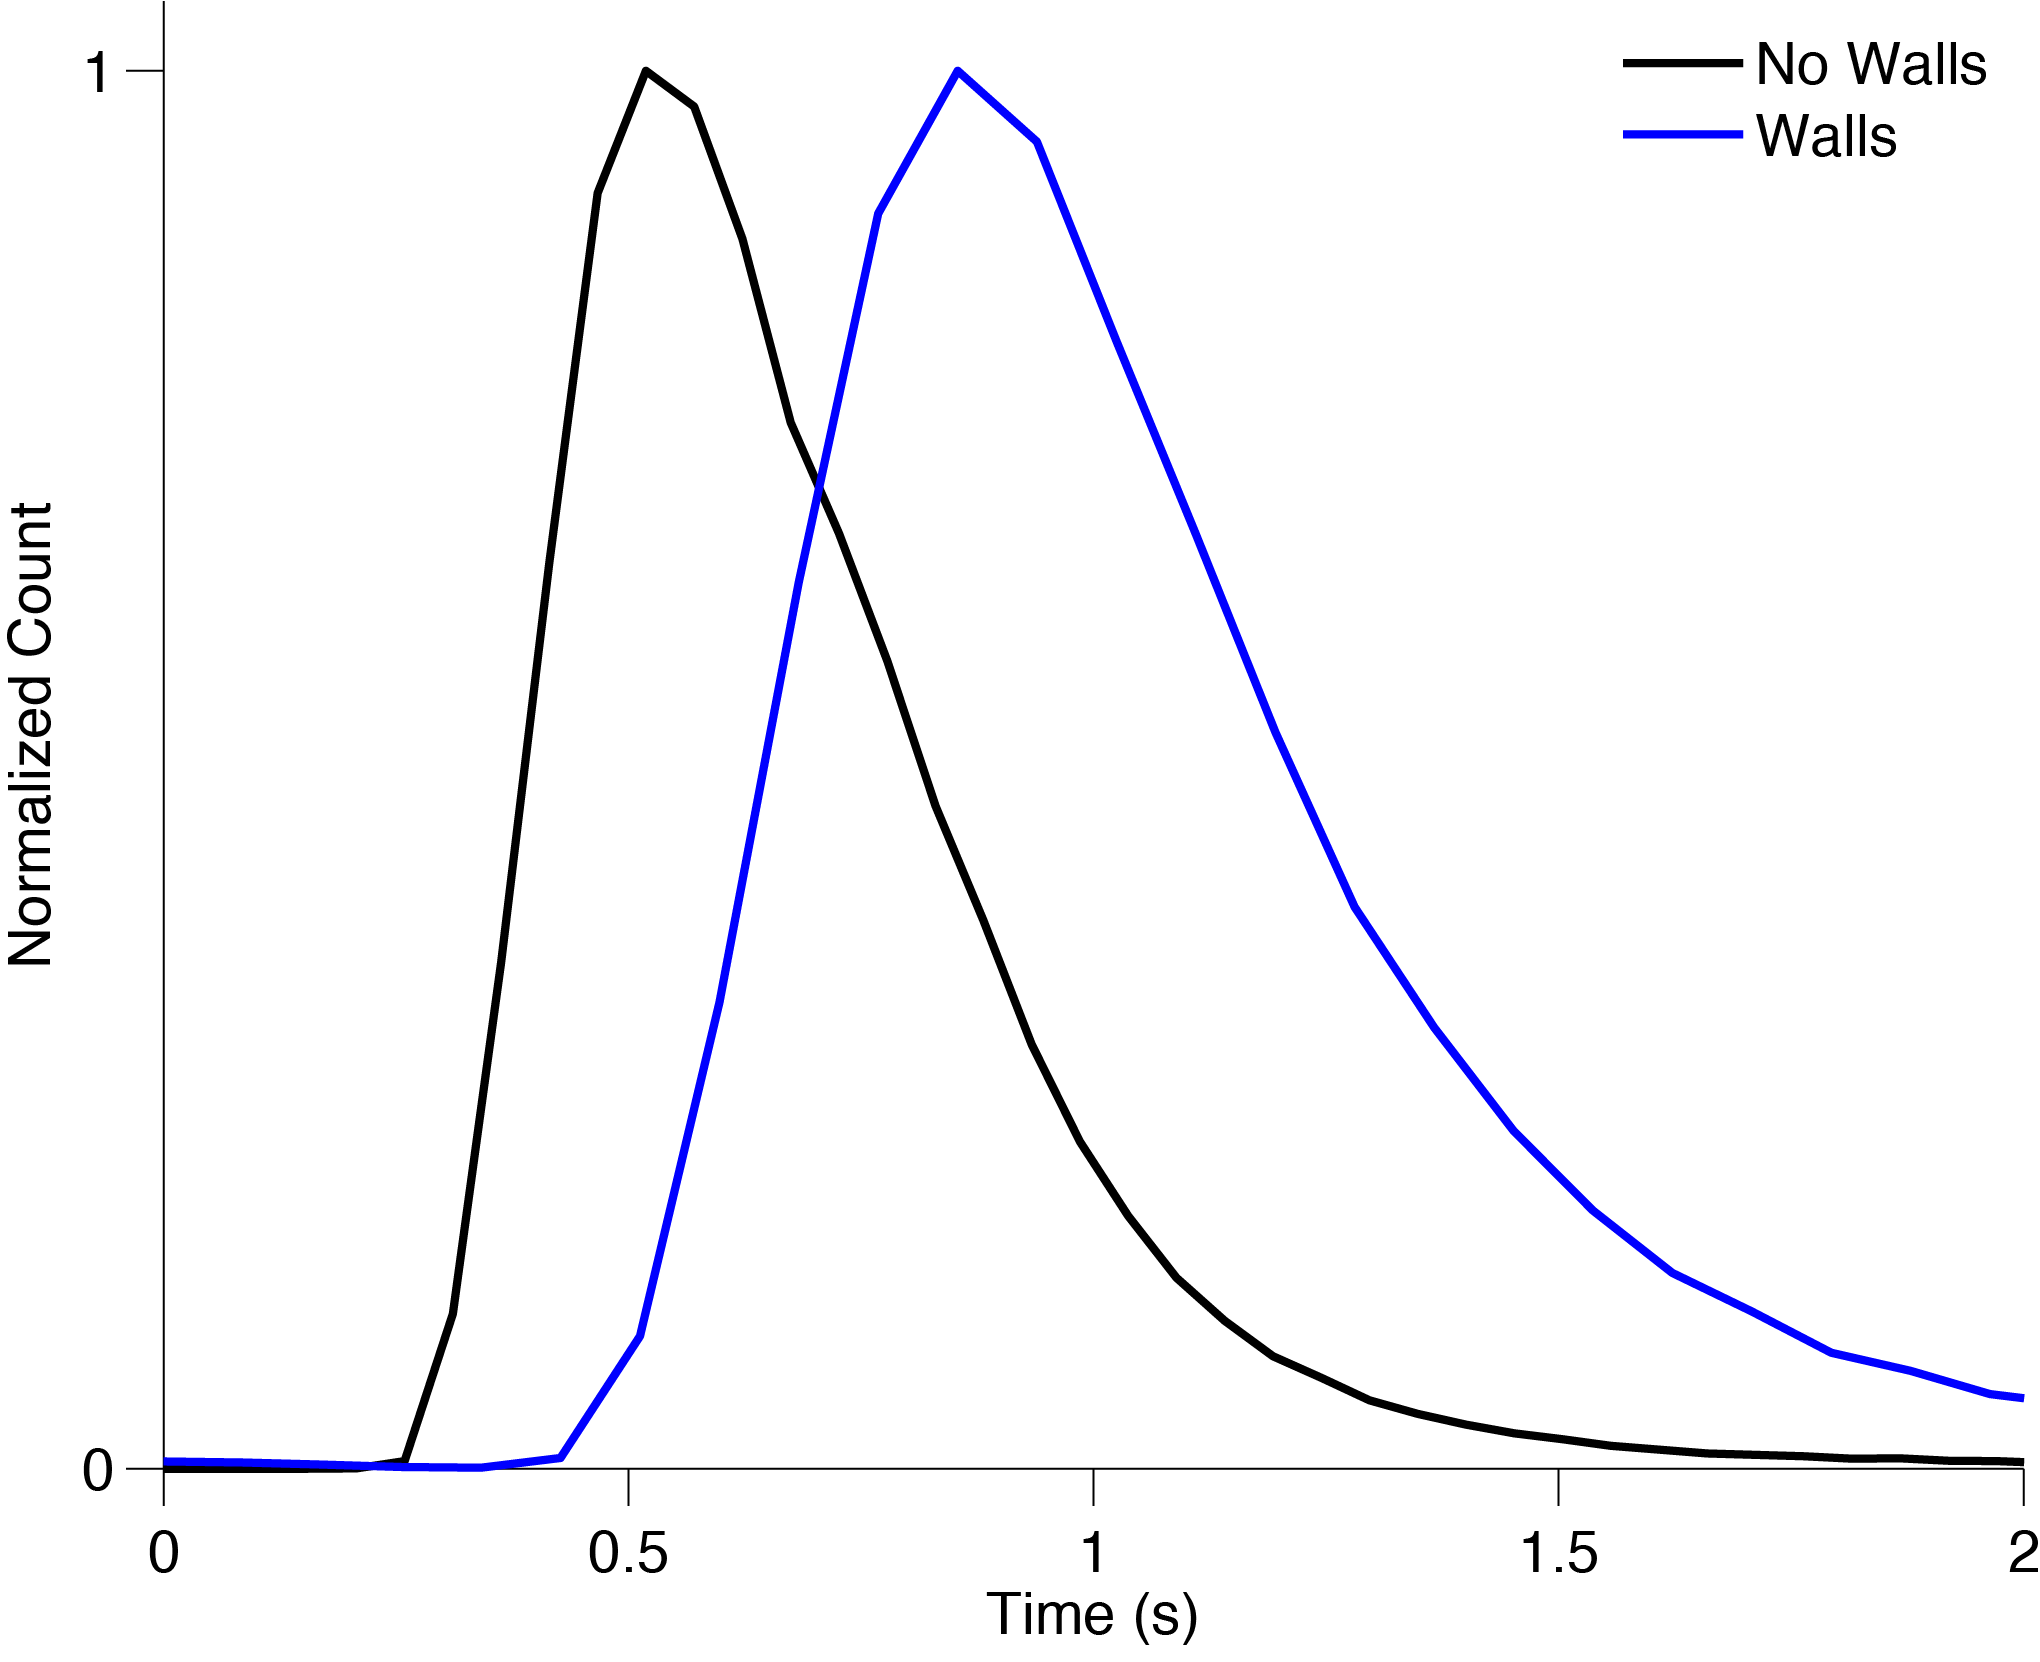
\includegraphics[width=\textwidth]{Figures/chapter2/RTHistogram_Combined.png}
  \caption[Response Time Histogram]{\textbf{Response Time Histogram} For mice trained with walls (blue, n = 10 mice) and without walls (black, n = 19 mice)}
   \label{fig:rthistogram}
\end{figure}
Mice trained with walls took much longer to reach the side reward ports than mice trained without the walls (Figure \ref{fig:rthistogram}). Similar to \textcite{Urai2017} we used the response time as our proxy for decision uncertainty. Surprisingly, there were differences in the uncertainty signatures between the two groups (Figures \ref{fig:rtuncertainty}). Response times from the mice trained with walls mirrored all three predictions of decision uncertainty (Figure \ref{fig:rtuncertainty} a-c). The performance accuracy decreased monotonically with response time (Spearman's correlation, $\rho$ = -1, p-value = 0.0167) (Figure \ref{fig:rtuncertainty}a). The mice responded more quickly on correct trials and responded more slowly on incorrect trials with increasing evidence strength  (Figure \ref{fig:rtuncertainty} b). Sensory evidence was calculated as the absolute difference between the flash rate and and the category boundary (12 flashes/s). Also, performance accuracy was greater on trials with higher response times (Figure \ref{fig:rtuncertainty} c). However, the response times from the second group of mice that were trained without walls and with an additional center reward did not recapitulate the predictions of decision uncertainty (Figure \ref{fig:uncertainty} d-f). \par 
\begin{figure}
  \centering
  	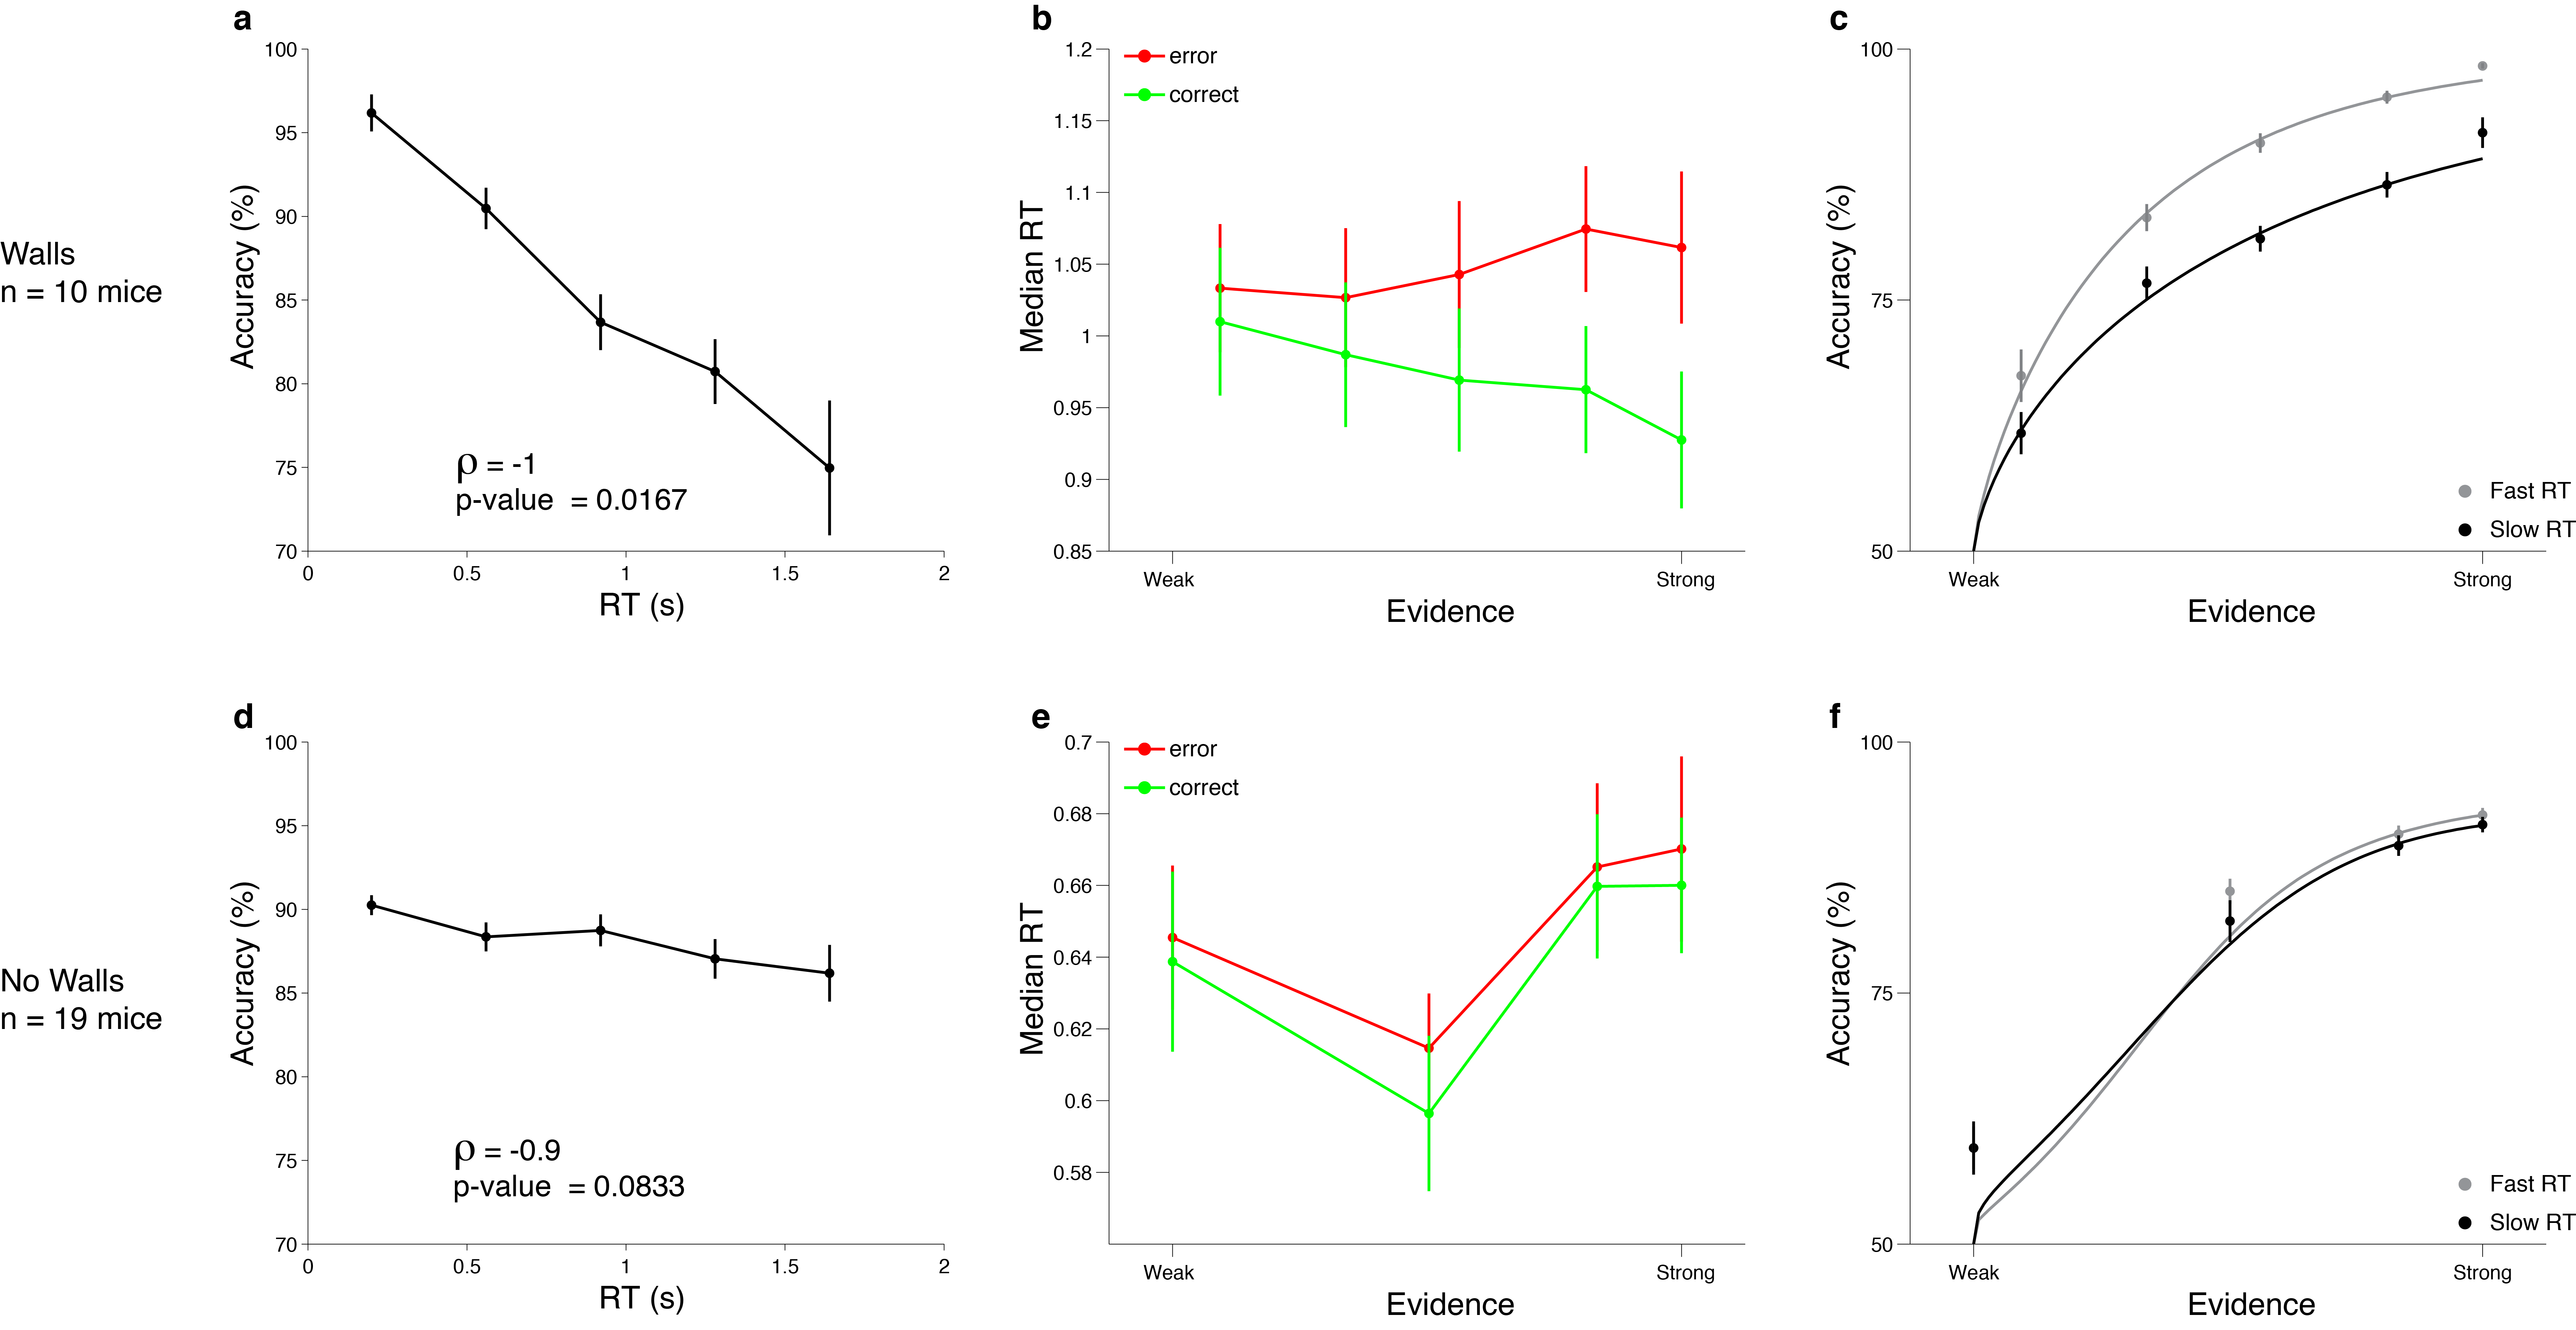
\includegraphics[width=\textwidth]{Figures/chapter2/RTUncertaintySignatures.png}
  \caption[Response Time and Decision Accuracy]{\textbf{Response Time and Decision Accuracy} Response time measured as the total time from Go-cue to side reward port. (First Row) Trained with walls n = 10 mice (Second Row) Trained without walls n = 19 mice. (a, d) Percent correct as a function of binned response times. (b,e) Median response time as a function of absolute sensory evidence. (c,f) Psychometric function for fast and slow response times. Error bars are SEM.}
   \label{fig:rtuncertainty}
\end{figure}
One explanation for the differences between the two groups is that signatures of perceptual uncertainty is associated with the cost to act. For the mice trained with walls, the cost is associated with moving around the physical barrier to the reward port. Hence, when the mouse is certain, they respond rapidly, and when uncertain it is more likely to guess. However, mice trained without the walls do not incur an additional movement and time cost in reaching towards the reward port. The cost, however, is associated with leaving the center port where they are also rewarded for waiting. Thus, the mice in this second group are more likely to spend less  time at the center port after the Go-cue when they are certain, and in most cases forgo the additional small center reward (0.5 $\mu$L) for the the larger side reward (2 $\mu$L). Conversely, when uncertainty is high the mouse will spend more time at the center port, harvesting the small center reward (the sure bet). To examine whether the three uncertainty signatures are present when response time is measured as additional time spent at the center port, I repeated the analyses in Figure \ref{fig:rtuncertainty} for the mice trained without walls. In Figure \ref{fig:rtuncertaintyNoWalls} a, the decision accuracy decreases monotonically with the additional time spent in the center (Spearman's correlation $\rho$=-1, p-value = 0.0833), consistent with the prediction that mice may forgo the small center reward when uncertainty is low and conversely spend more time harvesting the center reward when uncertainty is high. There was no difference between response time scaling with evidence for correct and error trials (Figure \ref{fig:rtuncertaintyNoWalls} b). However, accuracy was slightly higher for fast response times than slow response times (Figure \ref{fig:rtuncertaintyNoWalls} c).\par 
\begin{figure}
  \centering
  	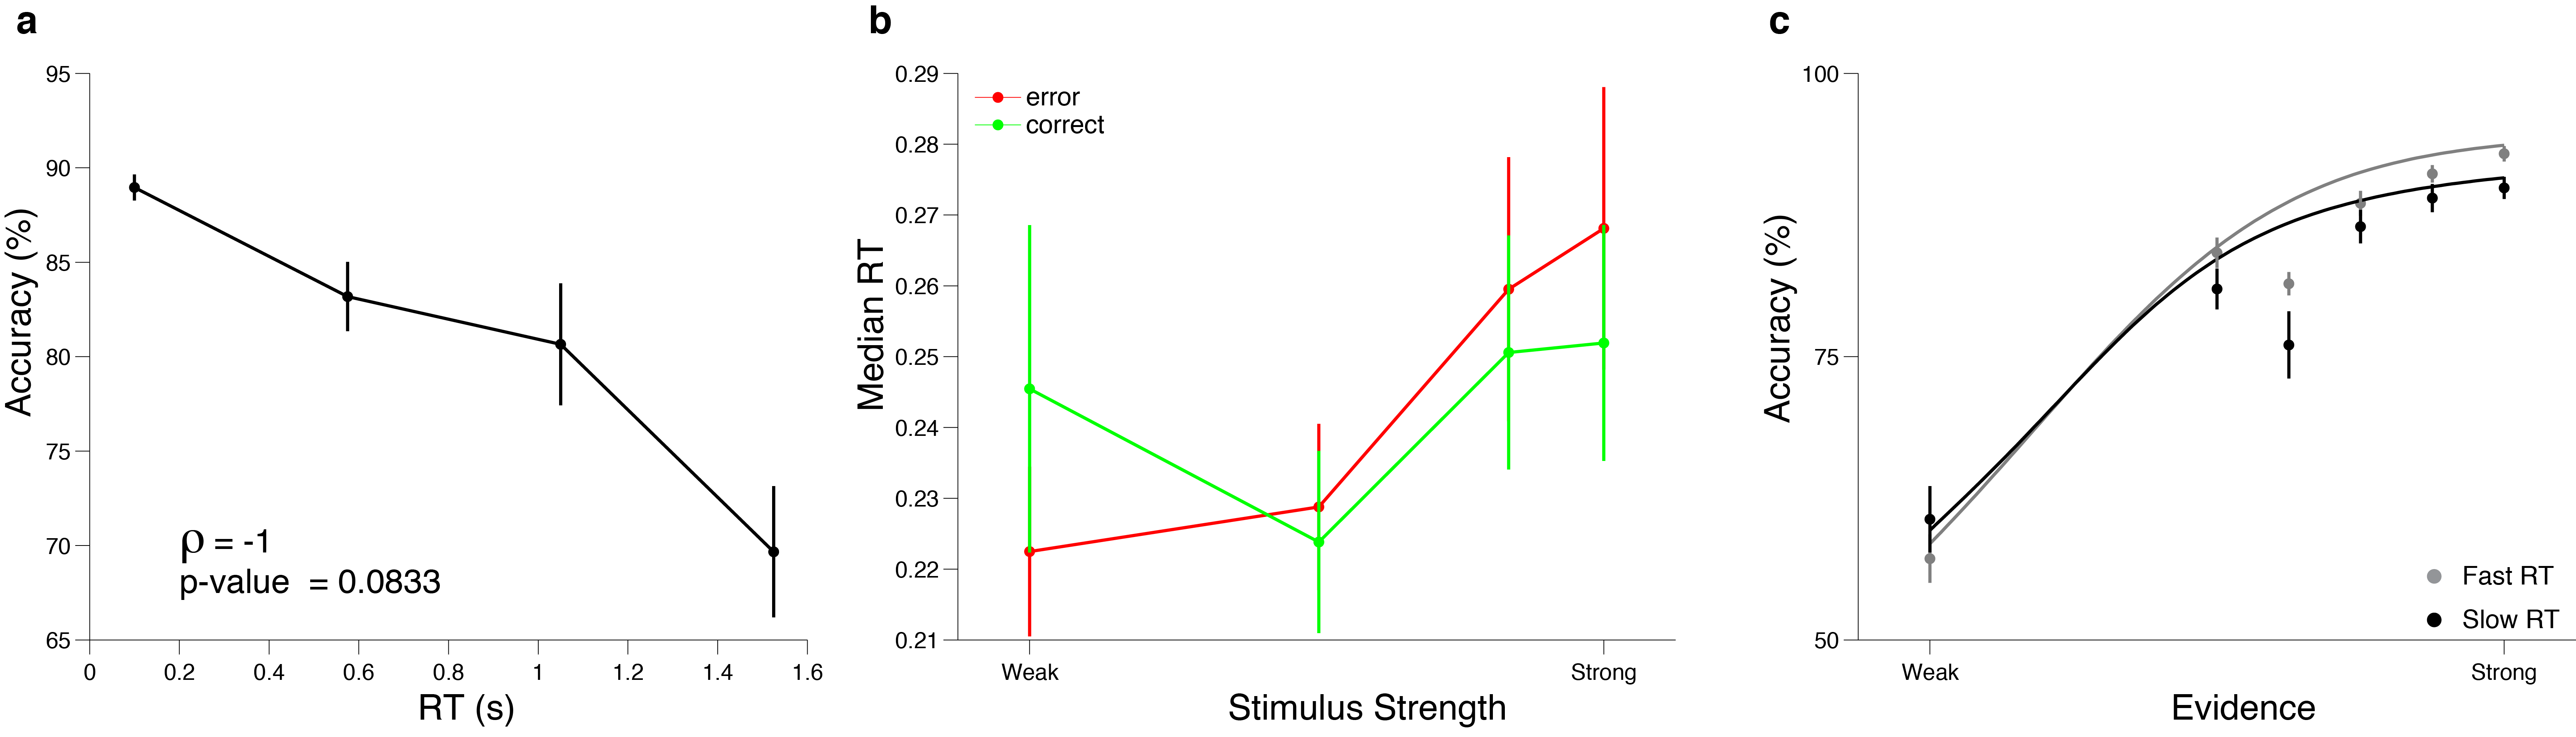
\includegraphics[width=\textwidth]{Figures/chapter2/RTUncertaintySignaturesNoWallsExtraCenter.png}
  \caption[Response Time and Decision Accuracy-No Walls]{\textbf{Response Time and Decision Accuracy} Response time measured as the additional time spent in the center port from Go-cue for mice trained without walls n = 19. (a) Percent correct as a function of binned response times. (b) Median response time as a function of absolute sensory evidence. (c) Psychometric function for fast and slow response times. Error bars are SEM.}
   \label{fig:rtuncertaintyNoWalls}
\end{figure}
These results indicate that for the mice trained without the walls and rewarded in the center, response time does not fully account for perceptual uncertainty as previously suggested by \textcite{Sanders2016}. With the current data, it is not clear whether the presence of the walls or the center liquid reward led to the presence or absence of signatures of behavioral uncertainty. An interesting experiment would be to directly test whether behavioral correlates of decision uncertainty are associated with the cost to act. One such way to test this with the current paradigm is to train mice with walls and reward in the center. Further, the center reward can be delivered on all trials or on a fraction of "catch" trials. \par 

\section{Discussion}
The focus of this chapter has been to provide a quantitative description of the behavior of mice performing an accumulation of visual evidence task. Such quantitative descriptions are important for generating and constraining mechanistic models of evidence accumulation. In the task, mice are presented with a rich stimulus set which allows them to explore and generalize across the stimulus space. Mice perform several hundreds of trials per session and maintain stable performance across sessions. In solving the task, the mice tend to deviate from an ideal strategy, whereby on average more weight was assigned to pulses presented earlier in trial, reflecting a snap judgment strategy. Similar to previous perceptual studies in humans and animals, mice trained on this paradigm were influenced by previous reward and choice history, further lending evidence that reward history is a source of behavioral variability or noise in visual evidence accumulation \parencite{Scott2015SourcesRats}. Lastly, the response times of mice trained with walls capture the signatures of decision uncertainty, whereas response times from mice trained without walls and rewarded in the center do not fully account for decision uncertainty. The difference in the two groups of mice suggests that the signatures of decision uncertainty might be influenced by the cost to act. 



 
% Chapter Template

\chapter{Chemogenetic Perturbation of Mouse Parietal Cortex} % Main chapter title

\label{Chapter3} 

One of the computational frameworks explaining how a neural circuit might implement evidence accumulation for decision making proposes a mechanism in which separate populations of neurons that modulate the net activity of the circuit in favor of (or against) a possible outcome of the decision. Inhibition plays a central role in these frameworks. For example, one class of models \parencite{Wang2002,Usher2001,Machens2005,Brown2001} suggests that inhibitory neurons mediate “competitive inhibition” between neuronal ensembles representing evidence in favor of a particular. Another class of decision making models \parencite{Ma2006,Beck2008} suggests that inhibitory neurons, alternatively, mediate global or “homeostatic inhibition” to normalize the responses of excitatory neurons in the population and prevent saturation. Although computational models involving inhibition are capable of recapitulating behavioral and neurophysiological results, \parencite{Usher2001,Wang2002,Machens2005,Beck2008,Wong2007,Wong2006} there is limited experimental evidence to support the computational roles of inhibitory neurons in perceptual evidence accumulation. An appealing possibility is that inhibitory neurons in the mouse posterior parietal cortex, a putative decision area, are involved in shaping evolving decisions.\par 
This chapter describes the approach to disrupting activity in mouse PPC in freely behaving animals and summarizes the behavioral impact of mouse PPC disruption. Silencing inhibitory neurons in mouse PPC significantly impaired the subjects' performance on the visual evidence accumulation task. These experiments also served as a means to test whether the behavioral paradigm engaged cortical machinery.
%----------------------------------------------------------------------------------------
%	SECTION 
%----------------------------------------------------------------------------------------
\section{Approach}
A chemogenetic approach called DREADD (Designer Receptor Exclusively Activated by Designer Drug, \textcite{Rogan2011}) was used to disrupt activity in mouse PPC (Figure \ref{fig:dreaddstrategy}). The DREADD approach was favored over other pharmacological methods such as muscimol because it offered a minimally invasive approach to reversibly perturbing neural activity. DREADDs also offers greater target specificity than muscimol, as it incorporates a fluorescent label which indicates where in the brain the receptors are expressed, and where the DREADD agonist (Clozapine-N-Oxide, CNO) will likely act.\par 

To target inhibitory neurons, I used a transgenic mouse line expressing Cre-recombinase in Gad2-positive (Gad2+) neurons, in combination with a Cre-dependent virus (AAV8-DIO-hSyn-hM4Di-mCherry) carrying the inhibitory DREADD receptor (hM4Di). Standard virus injection was used to introduce the DREADD receptor, bilaterally (Figure \ref{fig:dreaddexpression}) into the published stereotactic mouse PPC coordinates (2mm posterior and 1.7mm lateral from bregma, \textcite{Harvey2012}). Injection of the virus into mouse PPC restricts expression of the inhibitory DREADD to Gad2+ interneurons. Full expression took approximately 3-4 weeks from the date of injection. During this time the mice were allowed to recover and begin training on the task. The manipulation experiments were started once the mice acquired the task (approximately 6-8 weeks).The DREADD is activated by a pharmacologically inert designer drug, CNO (Clozapine-N-Oxide), which binds to the exogenous receptor, and in the case of the inhibibitory DREADD, hM4Di, suppresses neural activity. Before the start of a given session, we administered either saline (0.9\%) or CNO (2 mg/kg) via intraperitoneal injection.
\begin{figure}
  \centering
  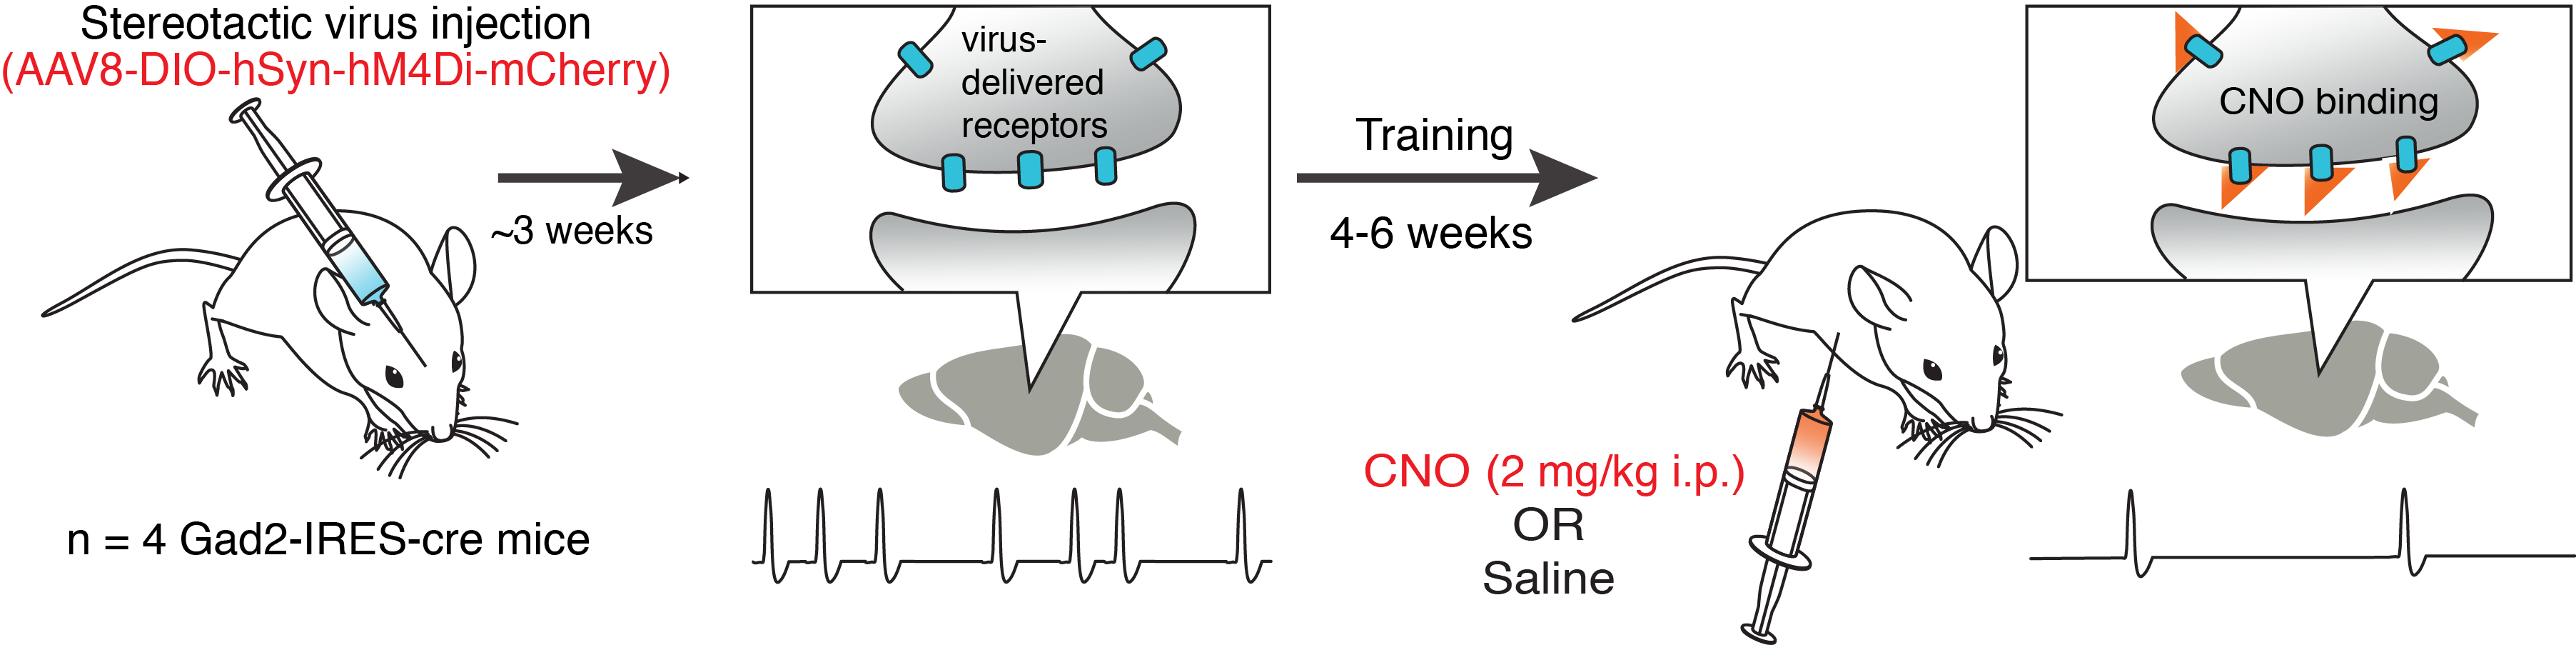
\includegraphics[width=\textwidth]{Figures/chapter3/DREADD_strategy.png}
  \caption[Strategy for Chemogenetic Manipulation of PPC]{\textbf{Strategy for Chemogenetic Manipulation of PPC.} Mice are injected with virus (AAV8-DIO-hSyn-hM4Di-mCherry) to express DREADD in PPC. Once the animals have acquired the decision task, they are given intraperitoneal injection of CNO or saline. Administration of CNO, activates the DREADD and reduces activity in cells expressing the receptor.}
   \label{fig:dreaddstrategy}
\end{figure}
\begin{figure}
  \centering
  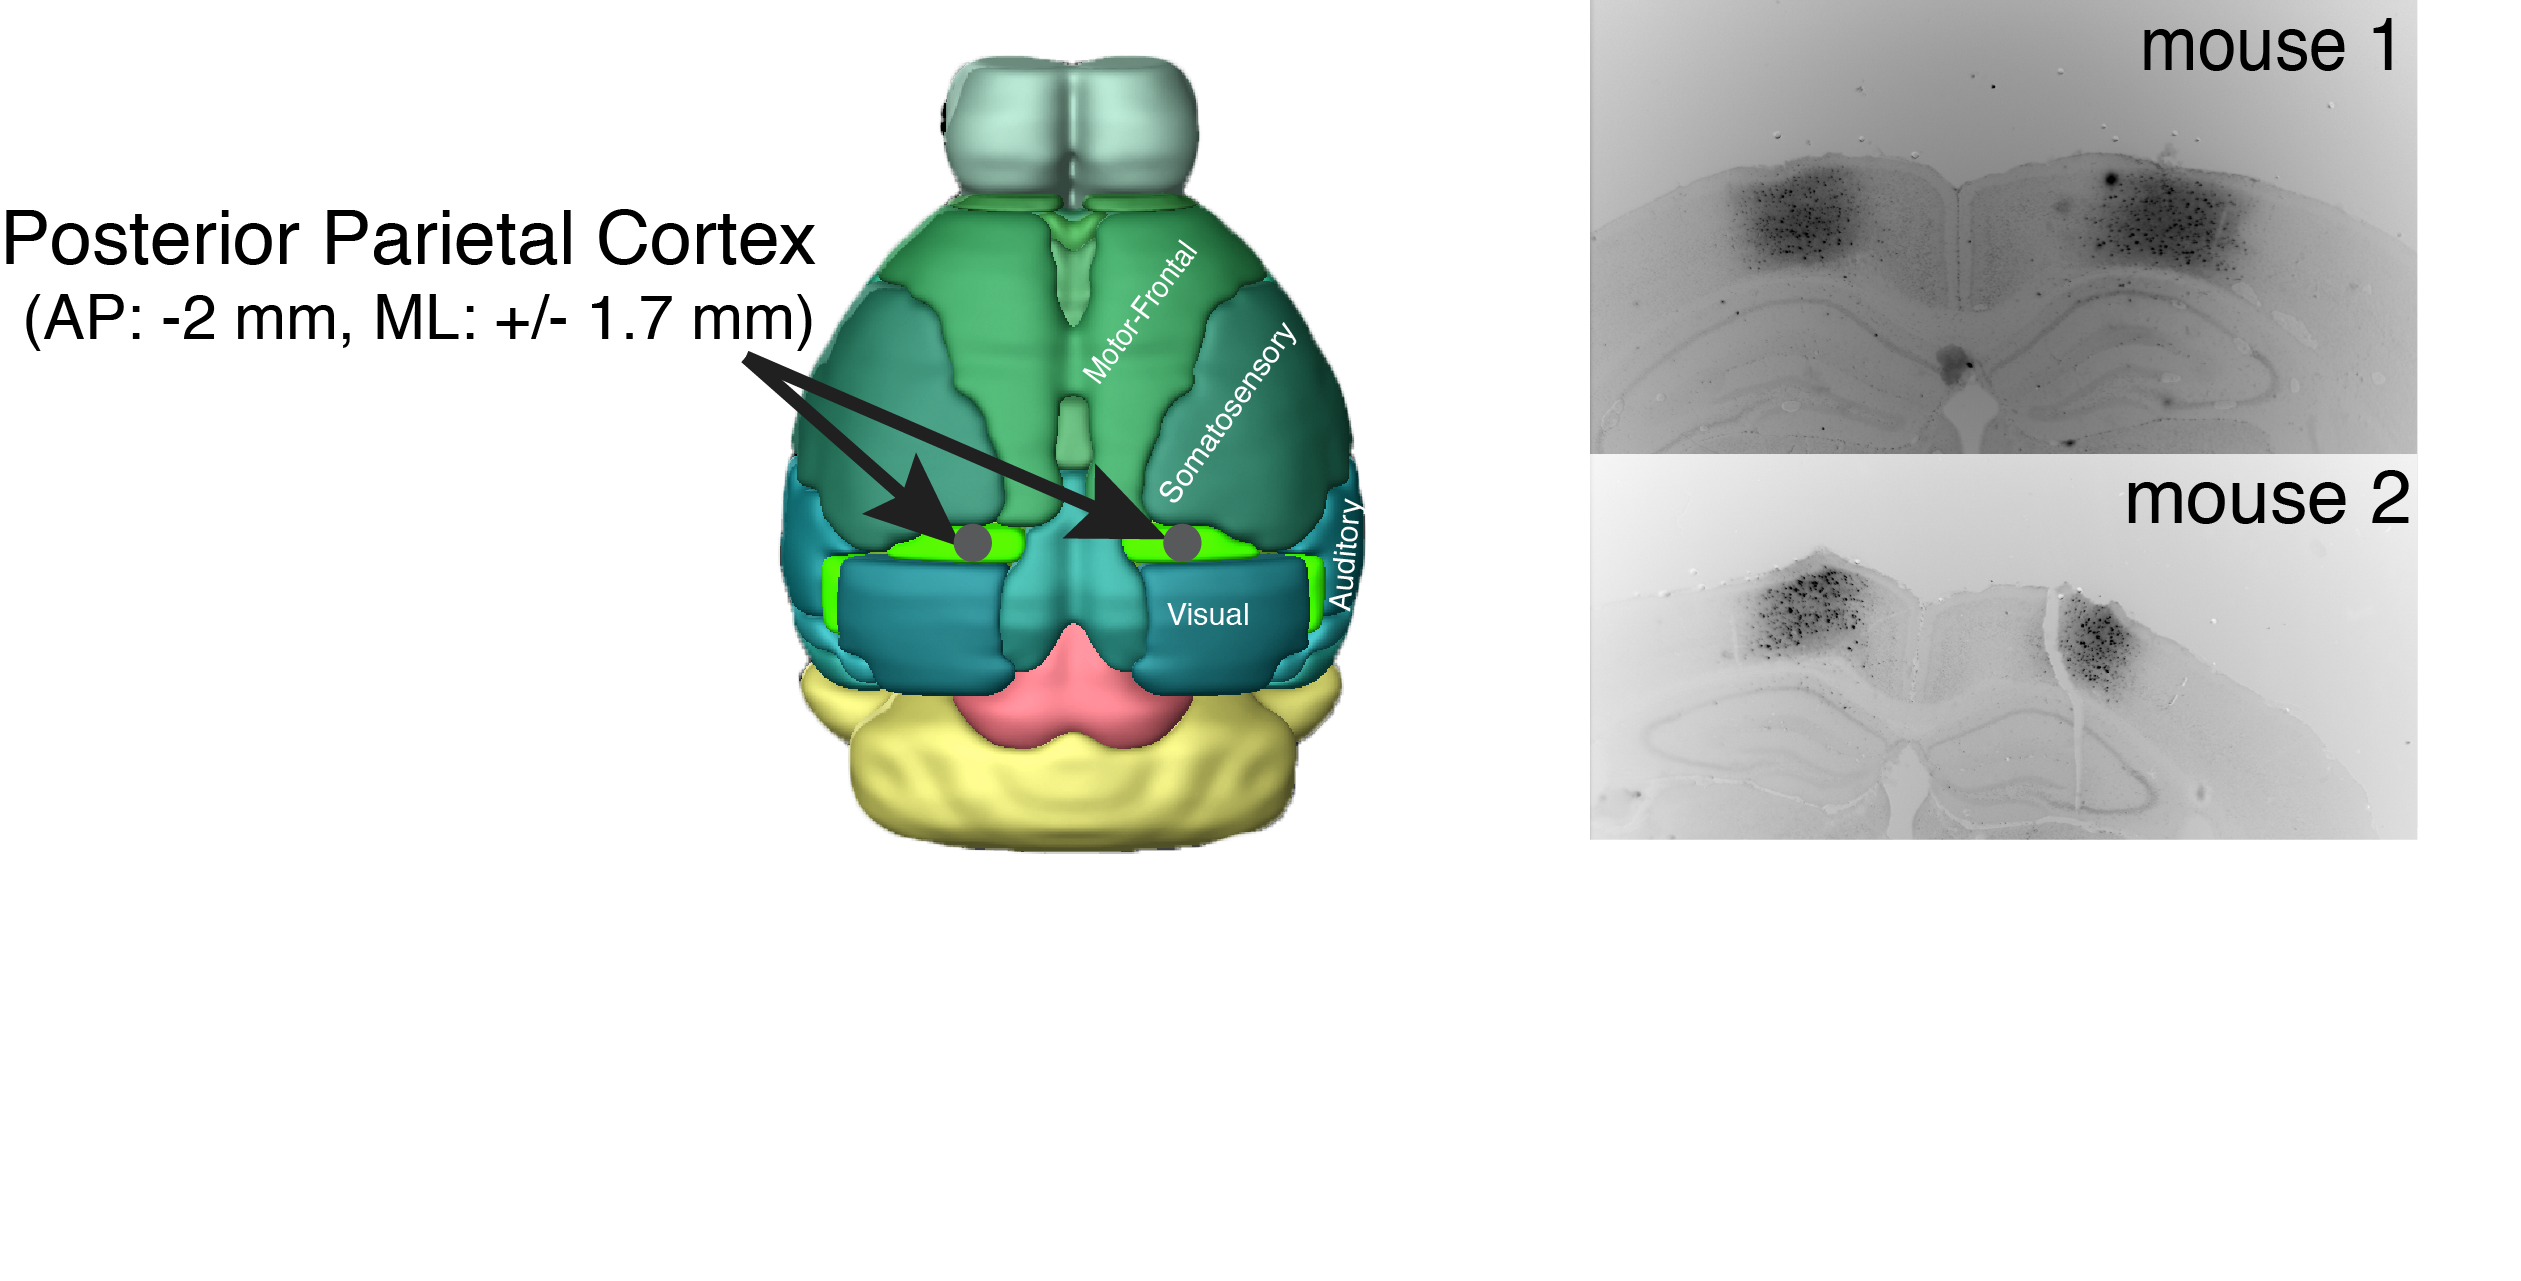
\includegraphics[width=\textwidth]{Figures/chapter3/DREADD_expression.png}
  \caption[Expression of inhibitory DREADD (hM4Di) in Gad+ neurons in PPC]{\textbf{Expression of inhibitory DREADD (hM4Di) in Gad+ neurons in PPC.} Fluorescence image of hM4Di-mCherry expression in mouse PPC for two example animals.}
   \label{fig:dreaddexpression}
\end{figure}
%----------------------------------------------------------------------------------------
%	SECTION 
%----------------------------------------------------------------------------------------
\section{DREADD silencing of PPC inhibitory neurons disrupts psychophysical performance}
Psychophysical performance of the mice expressing the DREADD receptor was reduced on CNO-treated sessions compared to saline control sessions (Figure \ref{fig:dreaddallmice}). The subjects' performance was quantified by estimating the slope of the psychometric curve function, which was fit with a cumulative Normal distribution (Psignifit). The width of the Gaussian ($\sigma$) reflects the inverse of the slope of the psychometric function and is related to the subject's sensitivity. Intuitively, the narrower the width of the Gaussian, the steeper the slope and the better the psychophysical performance. Conversely, the wider the Gaussian, the shallower the slope and the poorer the psychophysical performance. Across mice in this study, the slope of the psychometric function was much shallower on CNO treatment sessions compared to saline control sessions (Figure \ref{fig:dreaddallmice}c).\par 

Because the mice in Figure \ref{fig:dreaddallmice} were not trained to asymptotic performance before DREADD manipulation experiments, one concern is that the fit of the psychometric curve might yield poor estimates of the slope. Hence, performance was also quantified by estimating \emph{d'} (Equation \ref{dprime}), which is a signal detection theory index that quantifies the separation between the means of a signal and noise distribution \parencite{Macmillian,Green1989}.\emph{d'} is calculated according to the following equations:
\begin{equation}
\begin{aligned}	
    \centering
	d' &= \frac{\mu_H  - \mu_L}{\sqrt{0.5(\sigma^2_H + \sigma^2_L)}} \\
    d' &= Z(hit \: rate) - Z(false \: alarm)
\end{aligned}
\label{dprime}
\end{equation}
where $\mu$ and $\sigma$ represent the mean and the standard deviations of the high-rate (H) and low-rate (L) distributions; Z is the inverse cumulative Normal distribution. Intuitively, the higher the \emph{d'}, the better the psychophysical performance. Consistent with the estimates of the psychometric curve slope, \emph{d'} index was lower on CNO sessions compared to saline control sessions Figure \ref{fig:dreaddallmice}e.\par
\begin{figure}
  \centering
  	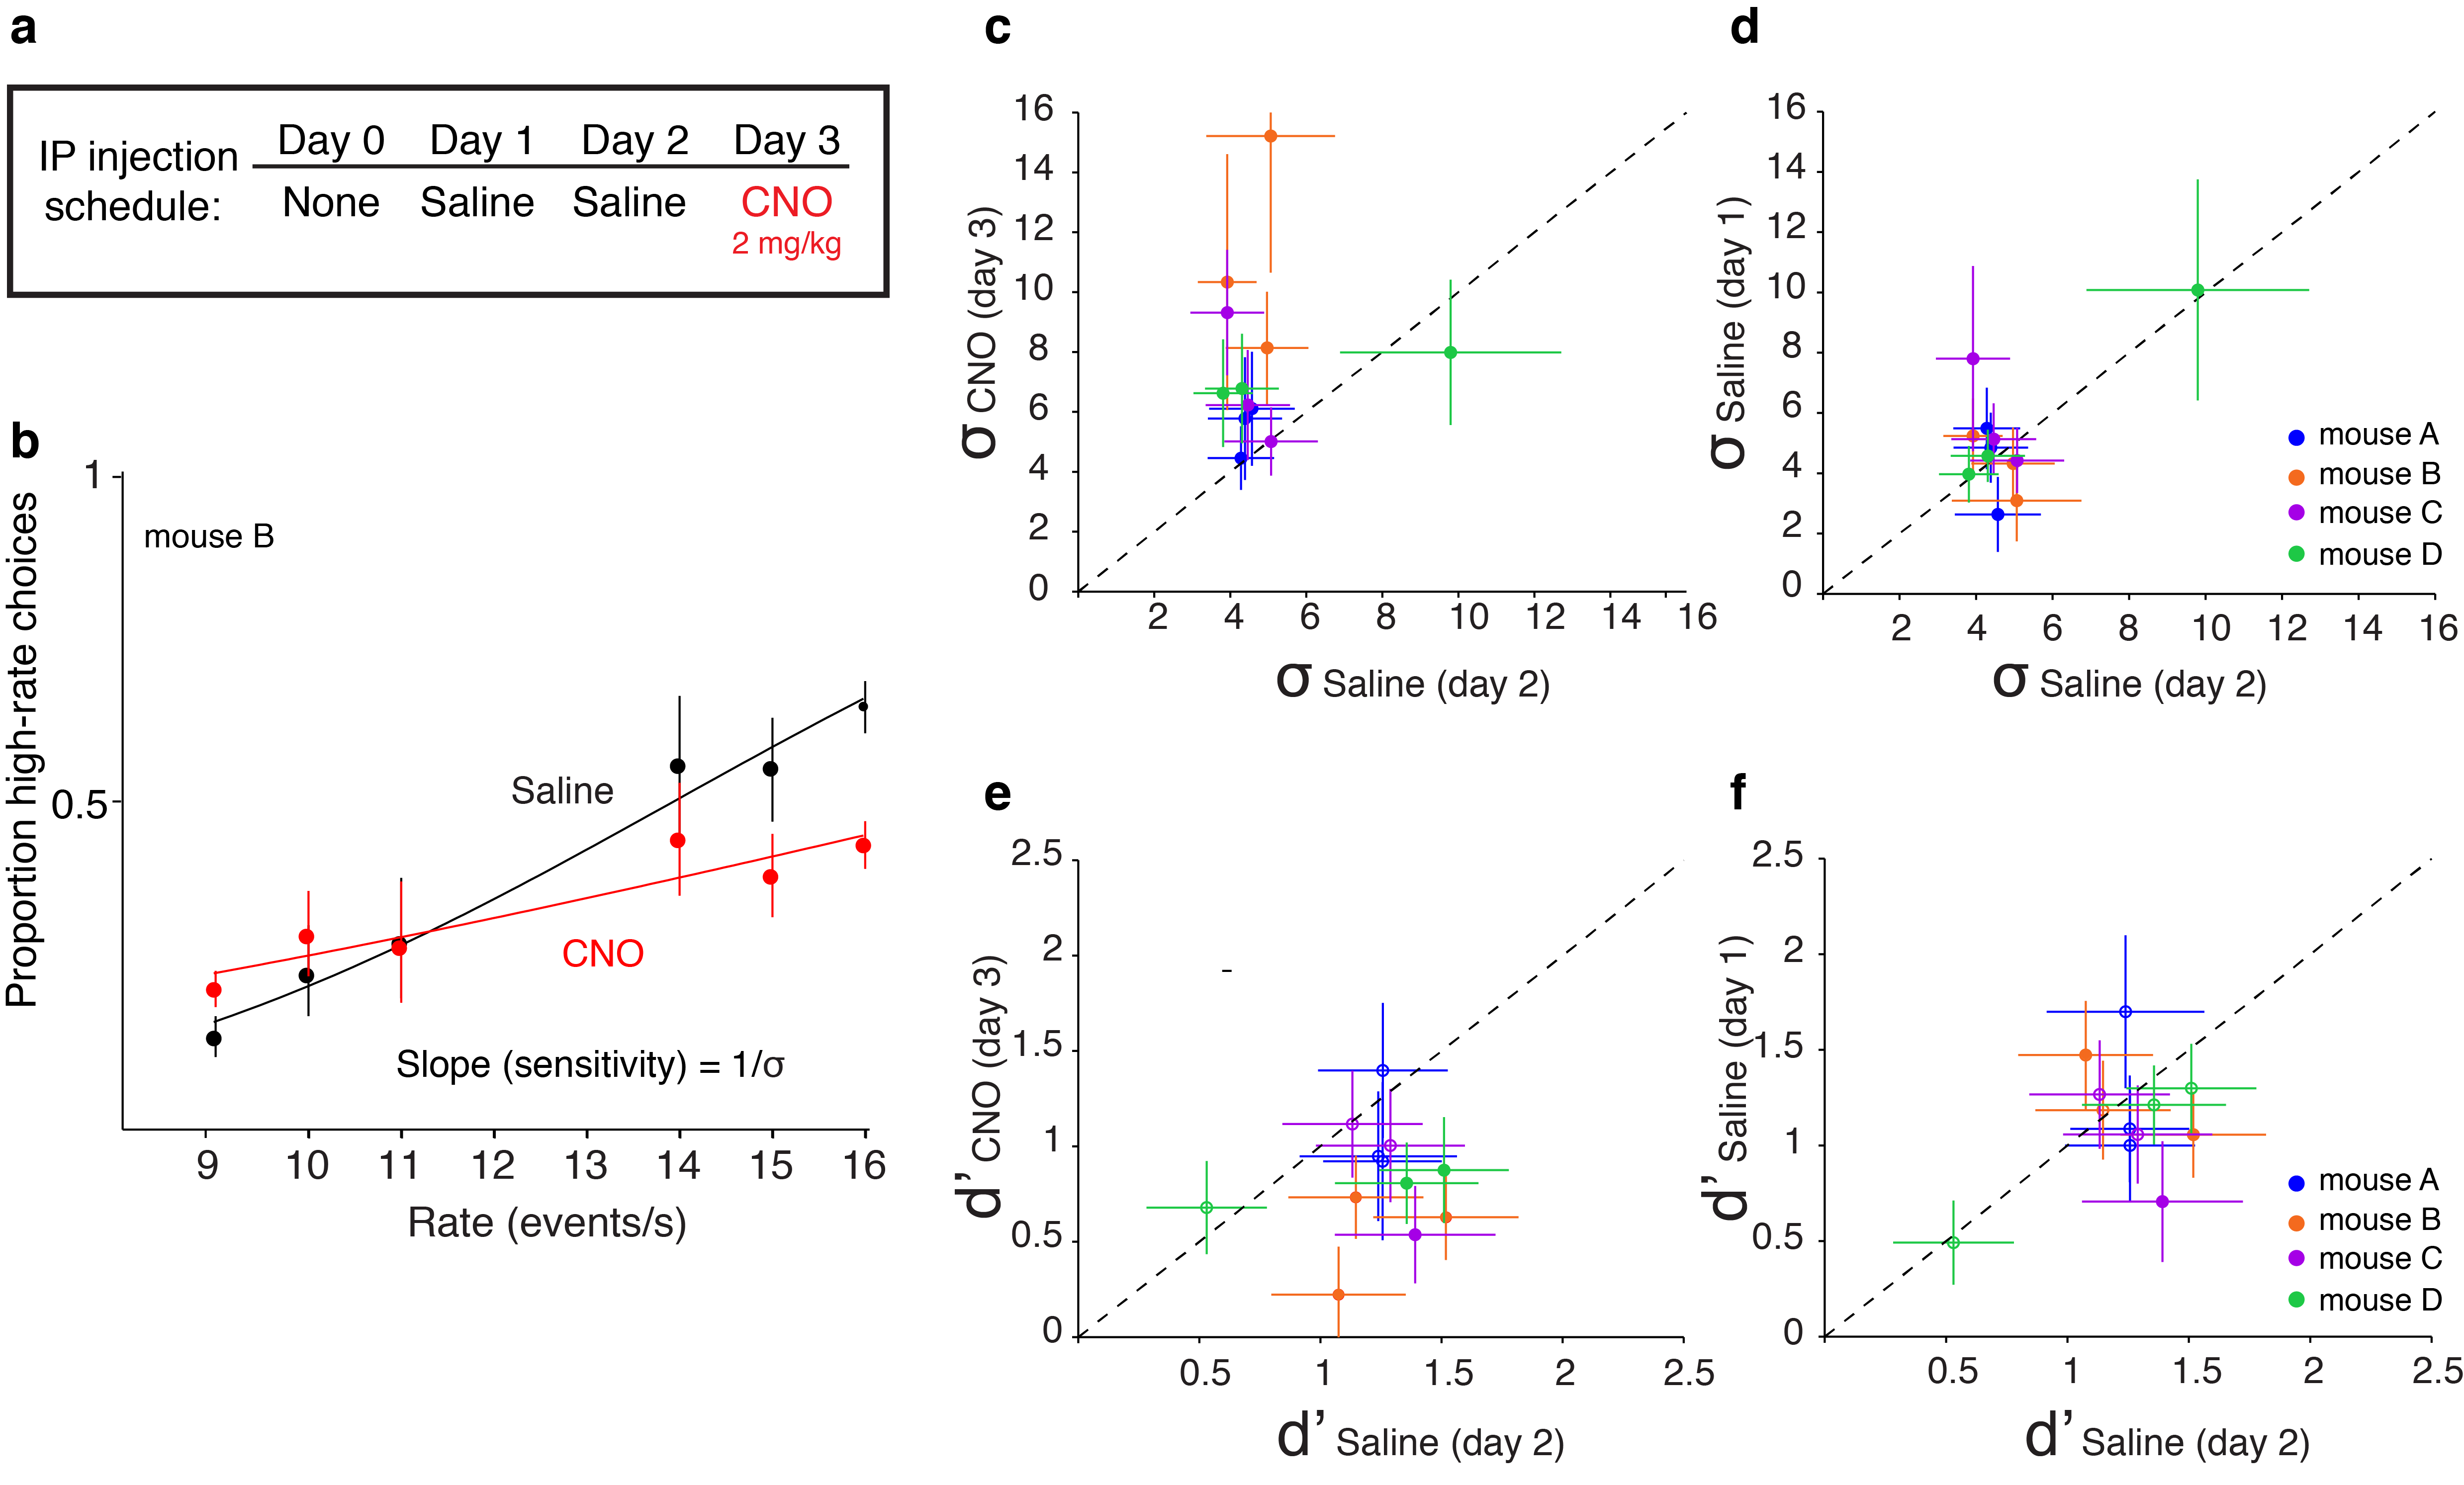
\includegraphics[width=\textwidth]{Figures/chapter3/psychophysics_dreadd_disruption.png}
  \caption[Chemogenetic silencing of mouse PPC disrupts psychophysical performance]{\textbf{Chemogenetic silencing of mouse PPC disrupts psychophysical performance.} (a) CNO and Saline treatment schedule. Saline typically administered two session prior to CNO treatment,(b) Mean psychometric performance of single mouse (n=3 CNO sessions, n= 3 saline sessions). (c) Summary of CNO vs. Saline control psychometric curve slope comparison (n=4 mice, 3 CNO/Saline sessions per mouse) shows performance impaired on CNO sessions compared to saline control sessions. (d) Summary comparison between two saline control days largely show no difference.(e) Comparison of d' on CNO vs saline control sessions also shows performance impairment on CNO sessions. (f) d' comparison of saline control sessions.}
  \label{fig:dreaddallmice}
\end{figure}
\begin{figure}
  \centering
  	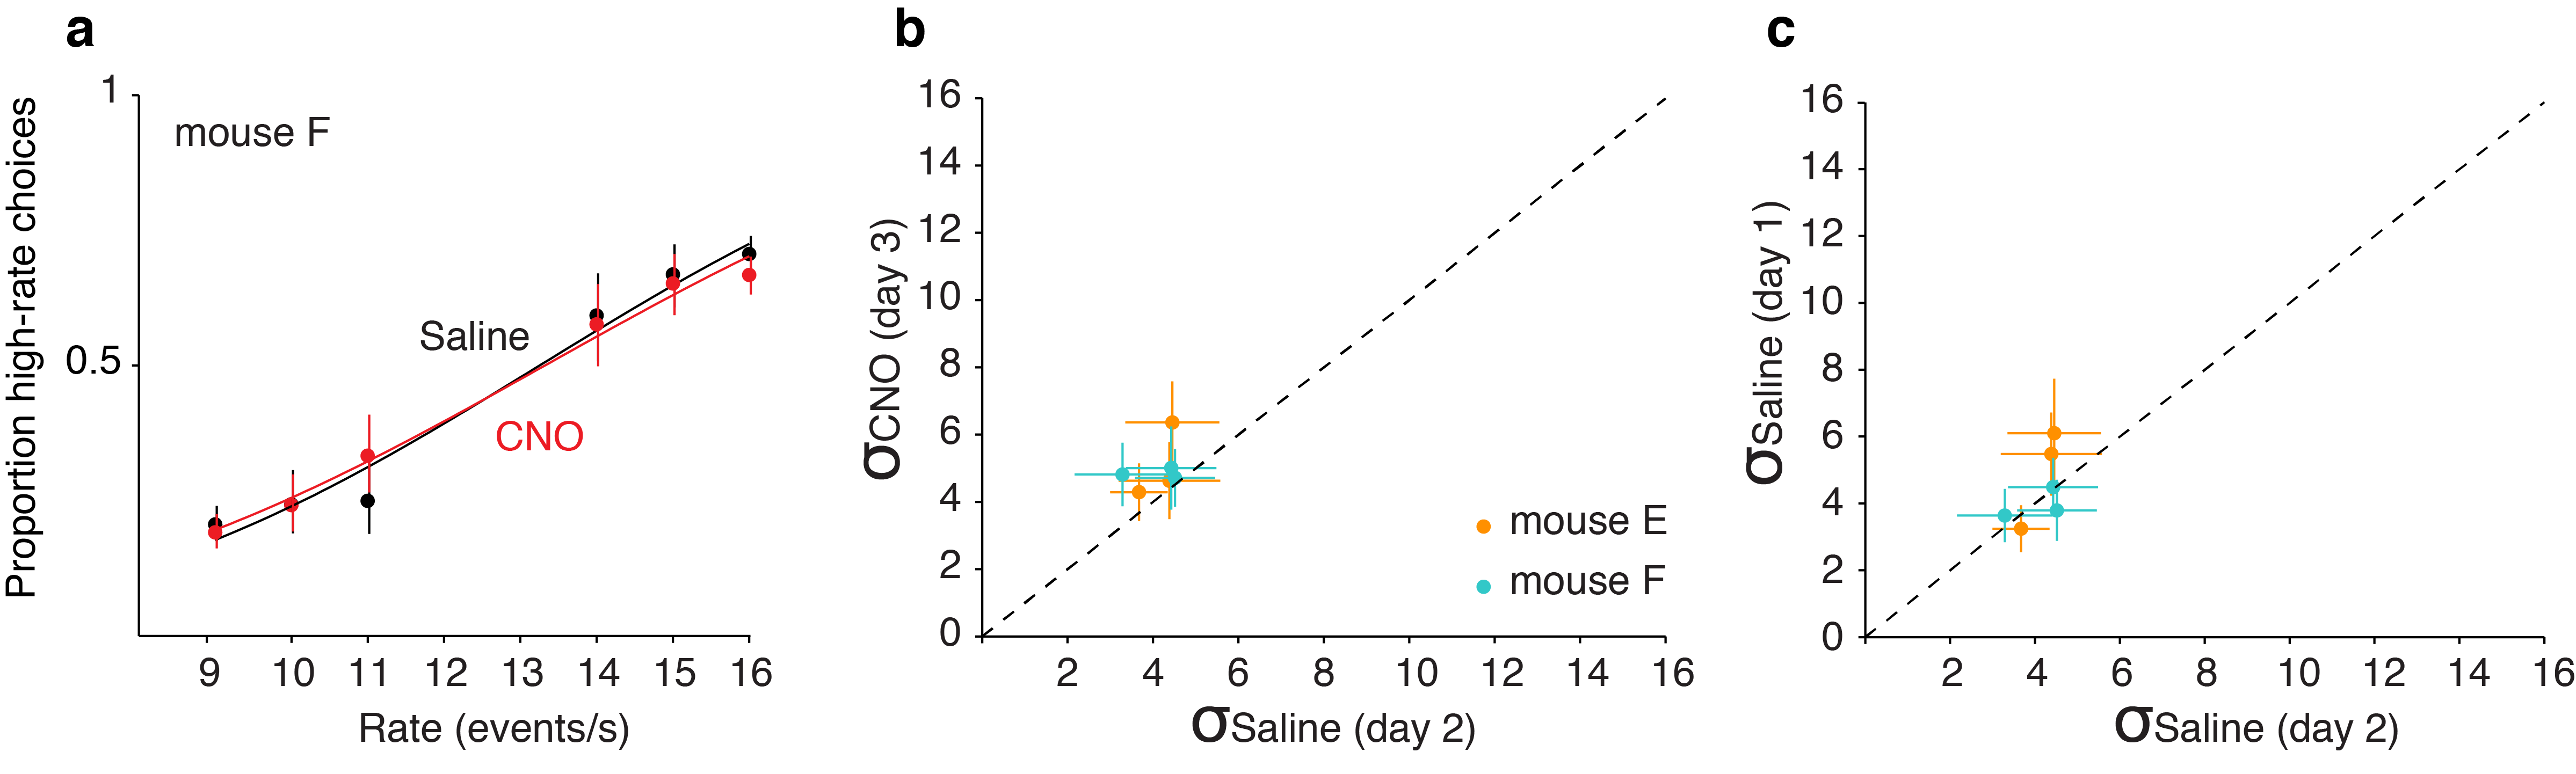
\includegraphics[width=\textwidth]{Figures/chapter3/dreadd_uninjected_control_mice.png}
  \caption[Uninjected DREADD virus control group]{\textbf{Uninjected DREADD virus control group.} CNO administration to wildtype animals did not affect decision-making accuracy. (a) Mean psychometric function of CNO-treated and saline treated sessions (n = 3 CNO/Saline sessions) for single mouse. Comparison of psychometric function slope (b) CNO- vs Saline-treated sessions, and (c) Saline vs. Saline-treated sessions.}
   \label{fig:dreaddcontrol}
\end{figure}
The disruption of psychophysical performance due to PPC DREADD manipulation could be explained by a number of factors. For instance, the behavioral impairment could be explained simply by the administration of CNO. To test this, I repeated the experiments in a cohort of wildtype mice (n = 2) that were not infected with DREADD receptor and observed no difference in psychophysical performance between CNO- and saline- treated sessions (Figure \ref{fig:dreaddcontrol}). Another plausible explanation for decreased psychophysical performance is that the mice failed to complete as many trials on CNO treatment sessions compared to saline sessions. However, mice completed just as many trials on CNO as on saline sessions and equally waited the minimum duration (1000 ms) before making a choice (Figure \ref{fig:dreaddtaskmeasures}a,b). However, the movement duration from the center port to the choice port was slightly slower on CNO treated sessions (Figure \ref{fig:dreaddtaskmeasures}c).\par 

\begin{figure}
  \centering
  	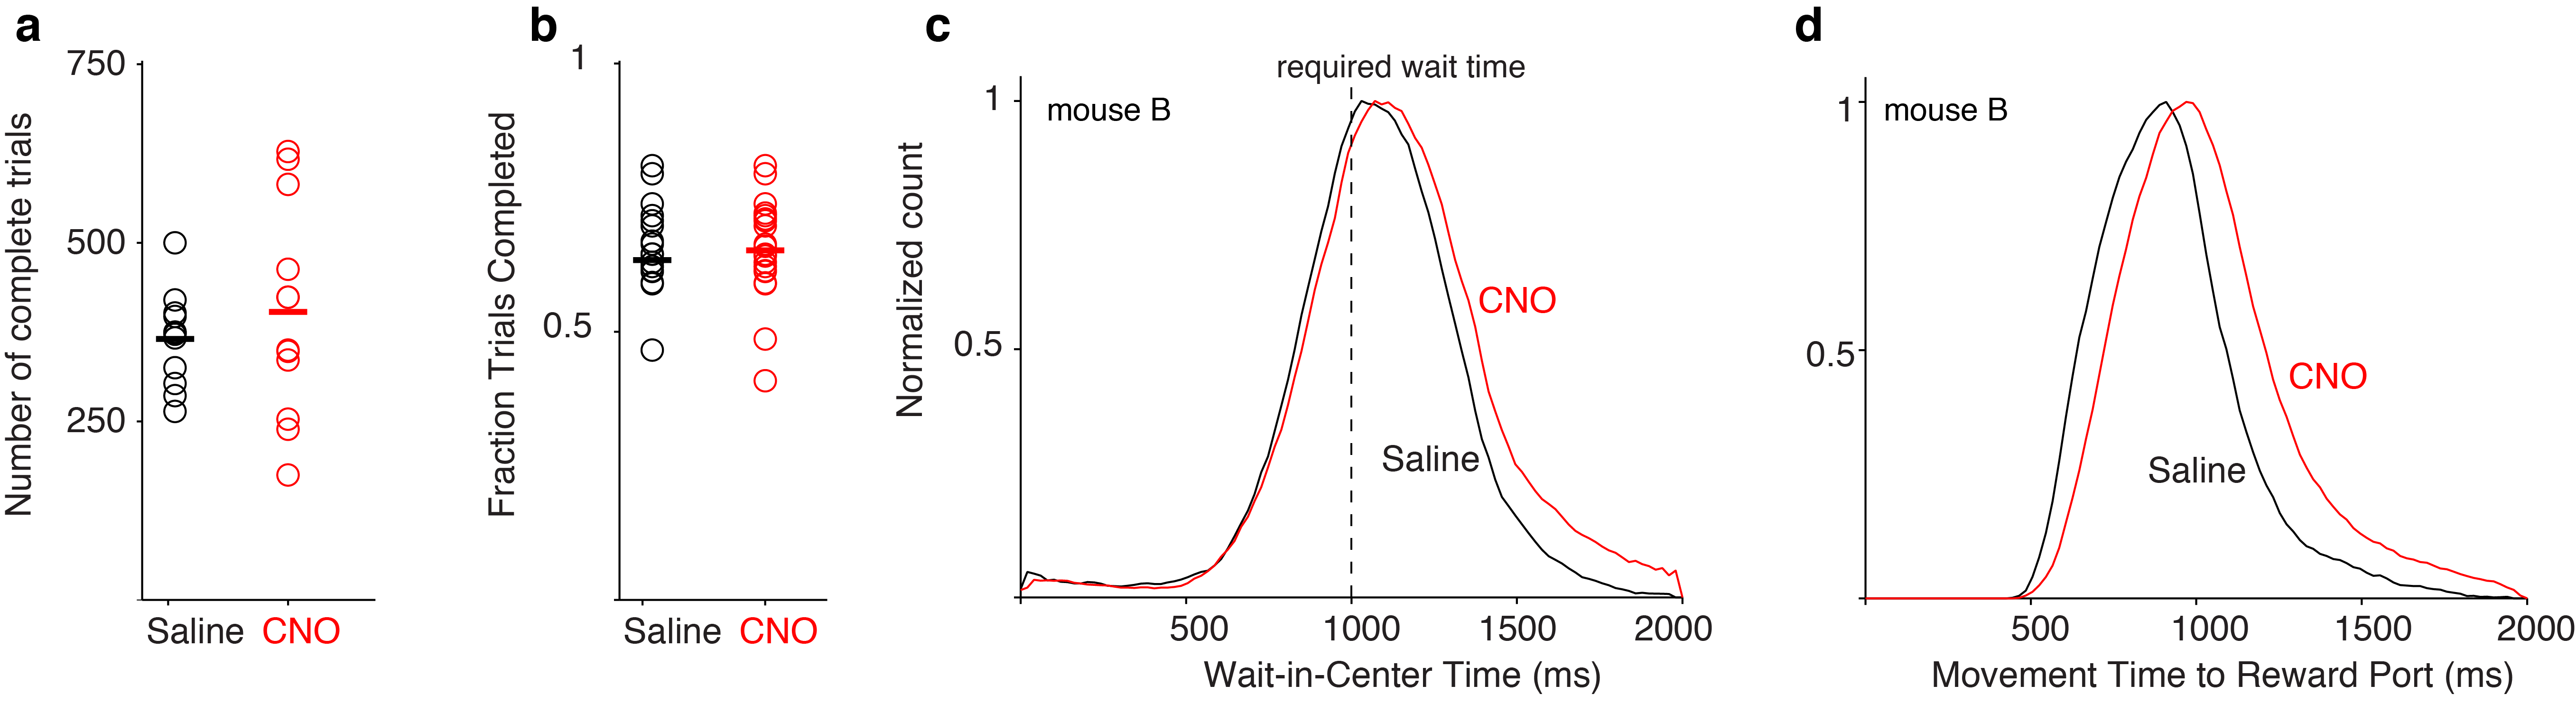
\includegraphics[width=\textwidth]{Figures/chapter3/non-stimulus_related_task_variables.png}
  \caption[Other task parameters unaffected by DREADD manipulation]{\textbf{Other task parameters unaffected by DREADD manipulation.} PPC manipulation  did not reduce the (a) number or (b) fraction of completed trials. (c) DREADD manipulation of PPC did not impair ability to wait the minimum required time before reporting choice. (d) PPC manipulation slightly increased movement duration to the reward port.}
   \label{fig:dreaddtaskmeasures}
\end{figure}
PPC DREADD manipulation could have differential effects during the course of a session. For example the CNO-induced DREADD perturbation could have a stronger effect early in the session, or conversely, it might take longer for the DREADD manipulation to take effect. To examine these potential scenarios, I compared the average percent correct performance across the first 200 trials (early) and the last 200 trials (late) (Figure \ref{fig:dreaddinsession}). Comparable decreases in performance were observed between early and late on CNO treated and saline control sessions.\par 
\begin{figure}
  \centering
  	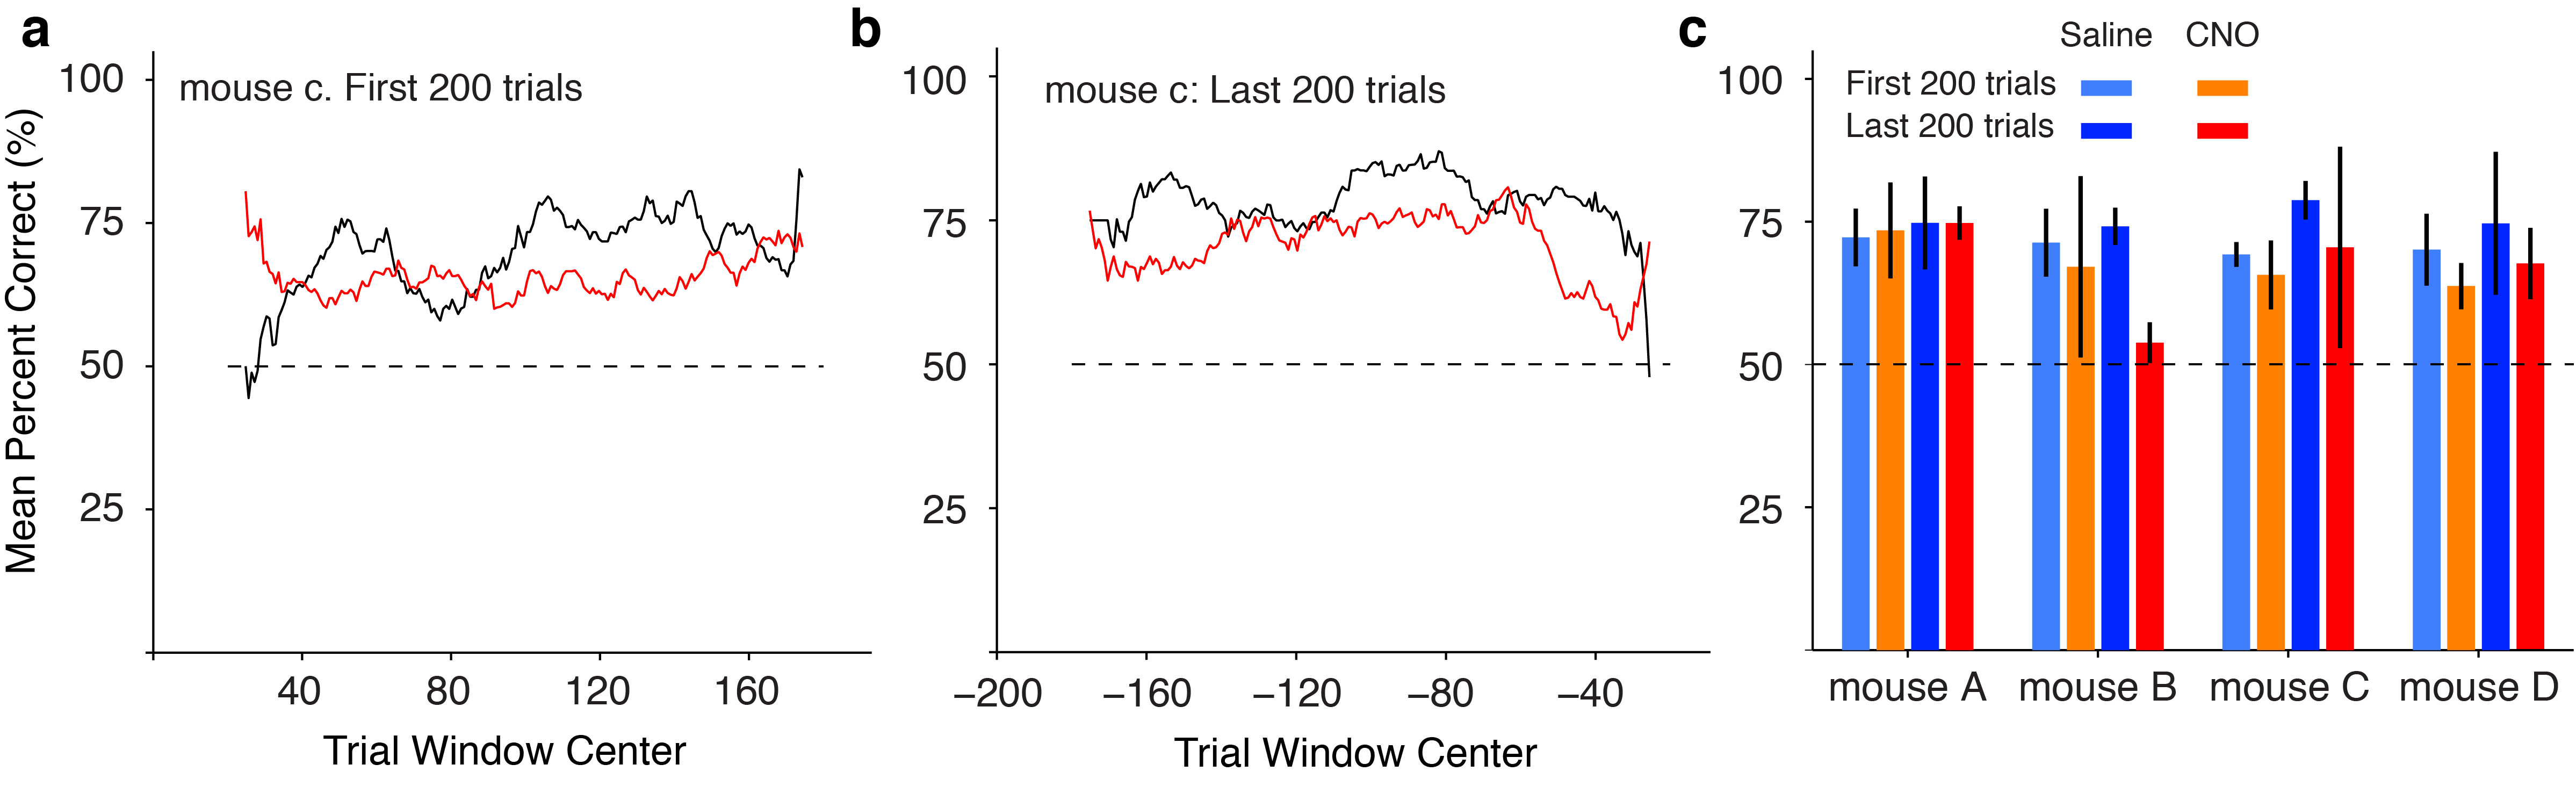
\includegraphics[width=\textwidth]{Figures/chapter3/within_session_comparison.png}
  \caption[Within session comparison of DREADD disruption]{\textbf{Within session comparison of DREADD disruption.} CNO treatment affected mean percent correct comparably for early and late in the session. Average percent correct across the (a) first 200 trials and (b) last 200 trials in session for single mouse. Black line represents control sessions. Red line represent CNO treatment sessions. (c) Average percent correct during first and last 200 trials for all mice.} 
   \label{fig:dreaddinsession}
\end{figure}
CNO is a reversible metabolite of the anti-psychotic drug, clozapine \parencite{Lin1994,Chang1998}. A potential concern was that higher doses and repeated exposure of the mice to CNO could have potential harmful and off target effects if CNO metabolized into clozapine. To evaluate the lifetime of CNO in the blood and to assess whether CNO metabolizes into clozapine, I collected blood serum from mice at different time points after CNO injection (Figure \ref{fig:dreaddcnoblood}). The blood serum was analyzed with mass spectroscopy at the CSHL Proteomics core facility. CNO clears the blood efficiently, in less than 20 minutes. There is also very minimal conversion of the CNO to clozapine. Our observation is consistent with a recent study \parencite{Guettier2009} that reported negligible conversion of CNO to clozapine. However, it is not clear how well the concentration of CNO in the blood relates to the amount of CNO (and/or clozapine) that enters the brain. 
\begin{figure}
  \centering
  	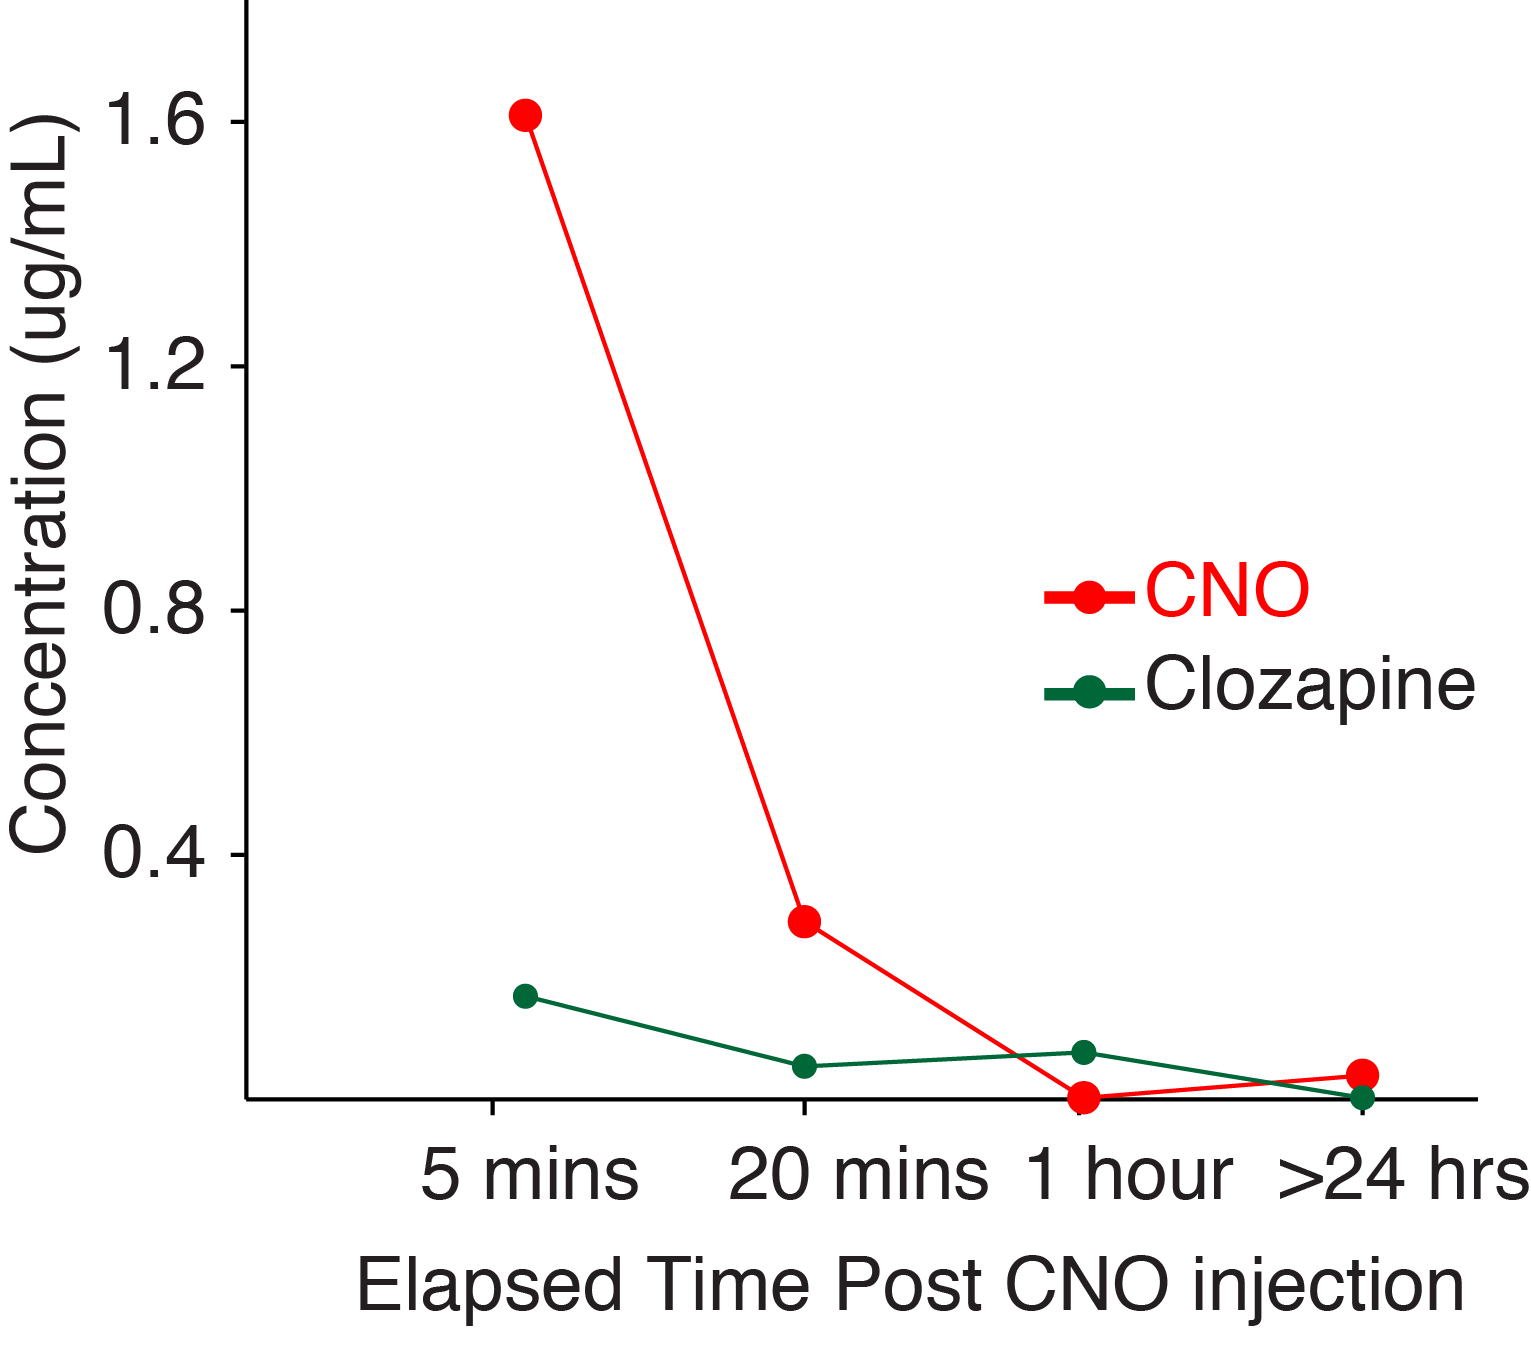
\includegraphics[scale=0.5]{Figures/chapter3/cno_lifetime_in_the_blood.png}
  \caption[CNO Lifetime in Blood Plasma]{\textbf{CNO Lifetime in Blood Plasma.} from an example mouse. CNO in the blood plasma rapidly decreases after IP injection.}
   \label{fig:dreaddcnoblood}
\end{figure}
\section{Discussion}
This chapter demonstrated that reversible chemogenetic disruption of mouse PPC by inhibition of inhibitory neurons reduced psychophysical performance. The result provides evidence that cortical machinery, in mice, plays a causal role in our visual evidence accumulation task. Chemogenetic disruption of mouse PPC did not impair the subjects' ability to execute the task, although the movement response time to the reward port was modestly reduced. In addition, control animals were not affected by CNO treatment in the absence of the DREADD receptor.\par 
The choice for PPC disruption was inspired by computational frameworks of perceptual decision making which highlight the role of inhibitory neurons in the neural implementation of the decision process \parencite{Beck2008,Wang2002}. Silencing inhibitory neurons is equivalent to adding aberrant noise to the circuit or tipping the cortical balance of excitation and inhibition (E/I balance) towards excitation. Inhibition is essential to shaping cortical computations \parencite{Haider2006,Haider2012,Isaacson2011}, and interfering with cortical balance of excitation-to-inhibition impacts local and global network activity and may underlie cognitive deficits \parencite{Markram2010,Rubenstein2010,Rubenstein2003,Yizhar2011}. Though simultaneous electrophysiological recordings were not performed to confirm the true nature of our chemogenetic PPC disruption, I speculate that the net effect on the circuit is increased local excitatory activity within PPC. If this is the case, the behavioral deficits observed in the mice are consistent with recent results from the Churchland lab \parencite{Licata2017}, which used an optogenetic strategy to directly elevate activity in rat PPC. In the \textcite{Licata2017} study, artificial excitatory drive in rat PPC also impaired accuracy on visual decisions, but had no effect on auditory decisions. These similar findings suggest a potentially conserved role for rodent PPC involvement in the process of evidence accumulation of visual decision making. 




% Chapter Template

\chapter{Optogenetic Inactivation of Mouse Visual Area AM} % Main chapter title
\label{Chapter4} 

The results of the previous chapter demonstrated that mouse cortex, namely the posterior parietal cortex, was necessary for accurate performance on the visual pulses task. However, the findings, which result from inactivation of inhibitory neurons, are not straightforward to interpret. Suppressing the activity of inhibitory neurons, in principle, results in increased excitation within the area that then alters the amount of activity that downstream brain areas experience. However the effect may also be restricted locally and may not recapitulate the neural activity resulting from exogenous drive approaches like those previously used to disrupt behavior in rodents \parencite{Otchy2015,Rodgers2014,Licata2017}.\par 

As discussed in the Introduction (Chapter \ref{Chapter1}), the definition of mouse PPC and it's location relative to retinotopic extrastriate visual areas is not firmly established. Previous studies that investigated mouse PPC \parencite{Harvey2012,Marcos2016,Funamizu2016,Goard2016,Jeong2017} do not report the boundary extent of mouse PPC (defined by stereotactic coordinates). Furthermore, while \textcite{Funamizu2016} referred to mouse PPC as the area anterior to visual area PM, most studies did not reconcile the location of mouse PPC with respect to known mouse secondary visual area. \par

In humans and primates, PPC is located in between the somatosensory and the visual cortex. In the mouse brain, this location is occupied by several retinotopic extrastriate visual areas \parencite{Wang2007,Zhuang2017}. The anatomical position and distinct projection targets of visual areas located between V1 and S1 (namely areas A, AM, RL,MMA, and RLL) open up the possibility that one or several of these retinotopic extrastriate visual areas may possess functional properties analogous with visual parietal areas previously annotated with in nonhuman primates \parencite{Cavada1993}. Because the boundary extent of stereotactic mouse PPC \parencite{Harvey2012} is undefined, it not obvious whether this area overlaps with one or more retinotopic visual areas. \par 

A promising candidate for mouse PPC, or subdivision thereof, is visual area AM. Area AM has prominent projection patterns to frontal and motor areas, which resemble those observed in primate LIP (Table \ref{table:areaLIP}), and is therefore, in a position to play a key role in conveying visual information into motor output. Few studies have examined how visual areas beyond V1 contribute to sensory driven behavior in mouse. Furthermore, the perceptual decision making field has not taken full advantage of the tools available in mouse for causally linking neural activity to behavior, namely, careful anatomical distinction of extrastriate areas combined with functional manipulations. These efforts present an opportunity to ascertain whether visual areas in the mouse show functional similarities to areas already defined in non-human primate.\par 

Towards this goal, the experiments in this chapter test the causal role of visual area AM (a proposed subdivision of mouse PPC ) in evidence accumulation for visually-guided behavior. Furthermore, the experiments aim towards the ultimate goal of establishing behavioral consequences for, otherwise largely unknown roles of, mouse extrastriate visual areas during behavior.\par 

% %--------------------------------------------------------------------------
% %--------------------------------------------------------------------------
\section{Projection Patterns of Visual Area AM}
The projection patterns of mouse visual area AM (Table \ref{table:areaAM}) resemble the patterns observed in primate area LIP (Table \ref{table:areaLIP}, \parencite{Cavada1989a,Cavada1989b,Cavada1989c}) and the projection patterns observed by \textcite{Harvey2012} for stereotactic mouse PPC (Table \ref{table:harveyPPC}). The data in Table \ref{table:areaAM} and Figure \ref{fig:areaAMprojections} was obtained from the Allen Brain Connectivity Atlas \parencite{AllenBrain2015}, in particular experiments in which intrinsic signal mapping was used to identify area AM and guide injection of the anterograde tracer (EGFP). For reference, the experiment id numbers are 528510546 and 518742338. The experiments differ in the volume of tracer injected in area AM (60nL and 200nL respectively). \par 

AM broadly projects to several visual areas including primary visual cortex (V1) (Figure \ref{fig:areaAMprojections}). Projections also include frontal and limbic areas including medial prefrontal (infralimbic, ILA and prelimbic, PL), orbitofrontal (ORB), anterior cingulate (ACA), and retrosplenial (RSP) cortices. AM targets several motor areas including primary and secondary motor cortices. Secondary motor cortex (MOs/M2) may contain the frontal orienting field (FOF), which is analogous to the primate FEF \parencite{Erlich2011,Barthas2017}. Interestingly, AM has pronounced projections to the striatum (STR), specifically the caudate putamen, even for small tracer volume injections. Although the projection from Area AM to the pons (P) is weak in small tracer volume injections, there is labeling of the cortical-spinal tract (cst). The anatomical projection targets of area AM, identified by retinotopic mapping, are compelling and qualify area AM as potential key player in visually-guided behavior. \par 
%--------------------------------------------------------------------
\begin{table}
\centering
\begin{tabular}{cl}
\hline
\multicolumn{2}{c}{Areas} \\ \hline
\textbf{Visual} & V1, LM, AL, AM,A, RL,POR,LI \\
\textbf{Motor} & M2 \\
\textbf{Frontal} & mPFC, Orbitofrontal \\
\textbf{Limbic} & Cingulate, Retrosplenial, Presubiculum \\
\textbf{Subcortical} & Striatum, Superior Colliculus, Pons \\ \hline
\end{tabular}
\caption[Visual Area AM Projection Target Summary]{\textbf{Visual Area AM Projection Target Summary} Data summarized from the Allen Institute Brain Connectivity Atlas \parencite{AllenBrain2015}; experiment id: 528510546 and 518742338.}
\label{table:areaAM}
\end{table}
%-----------------------------------------------------------------
\begin{figure}
  \centering
   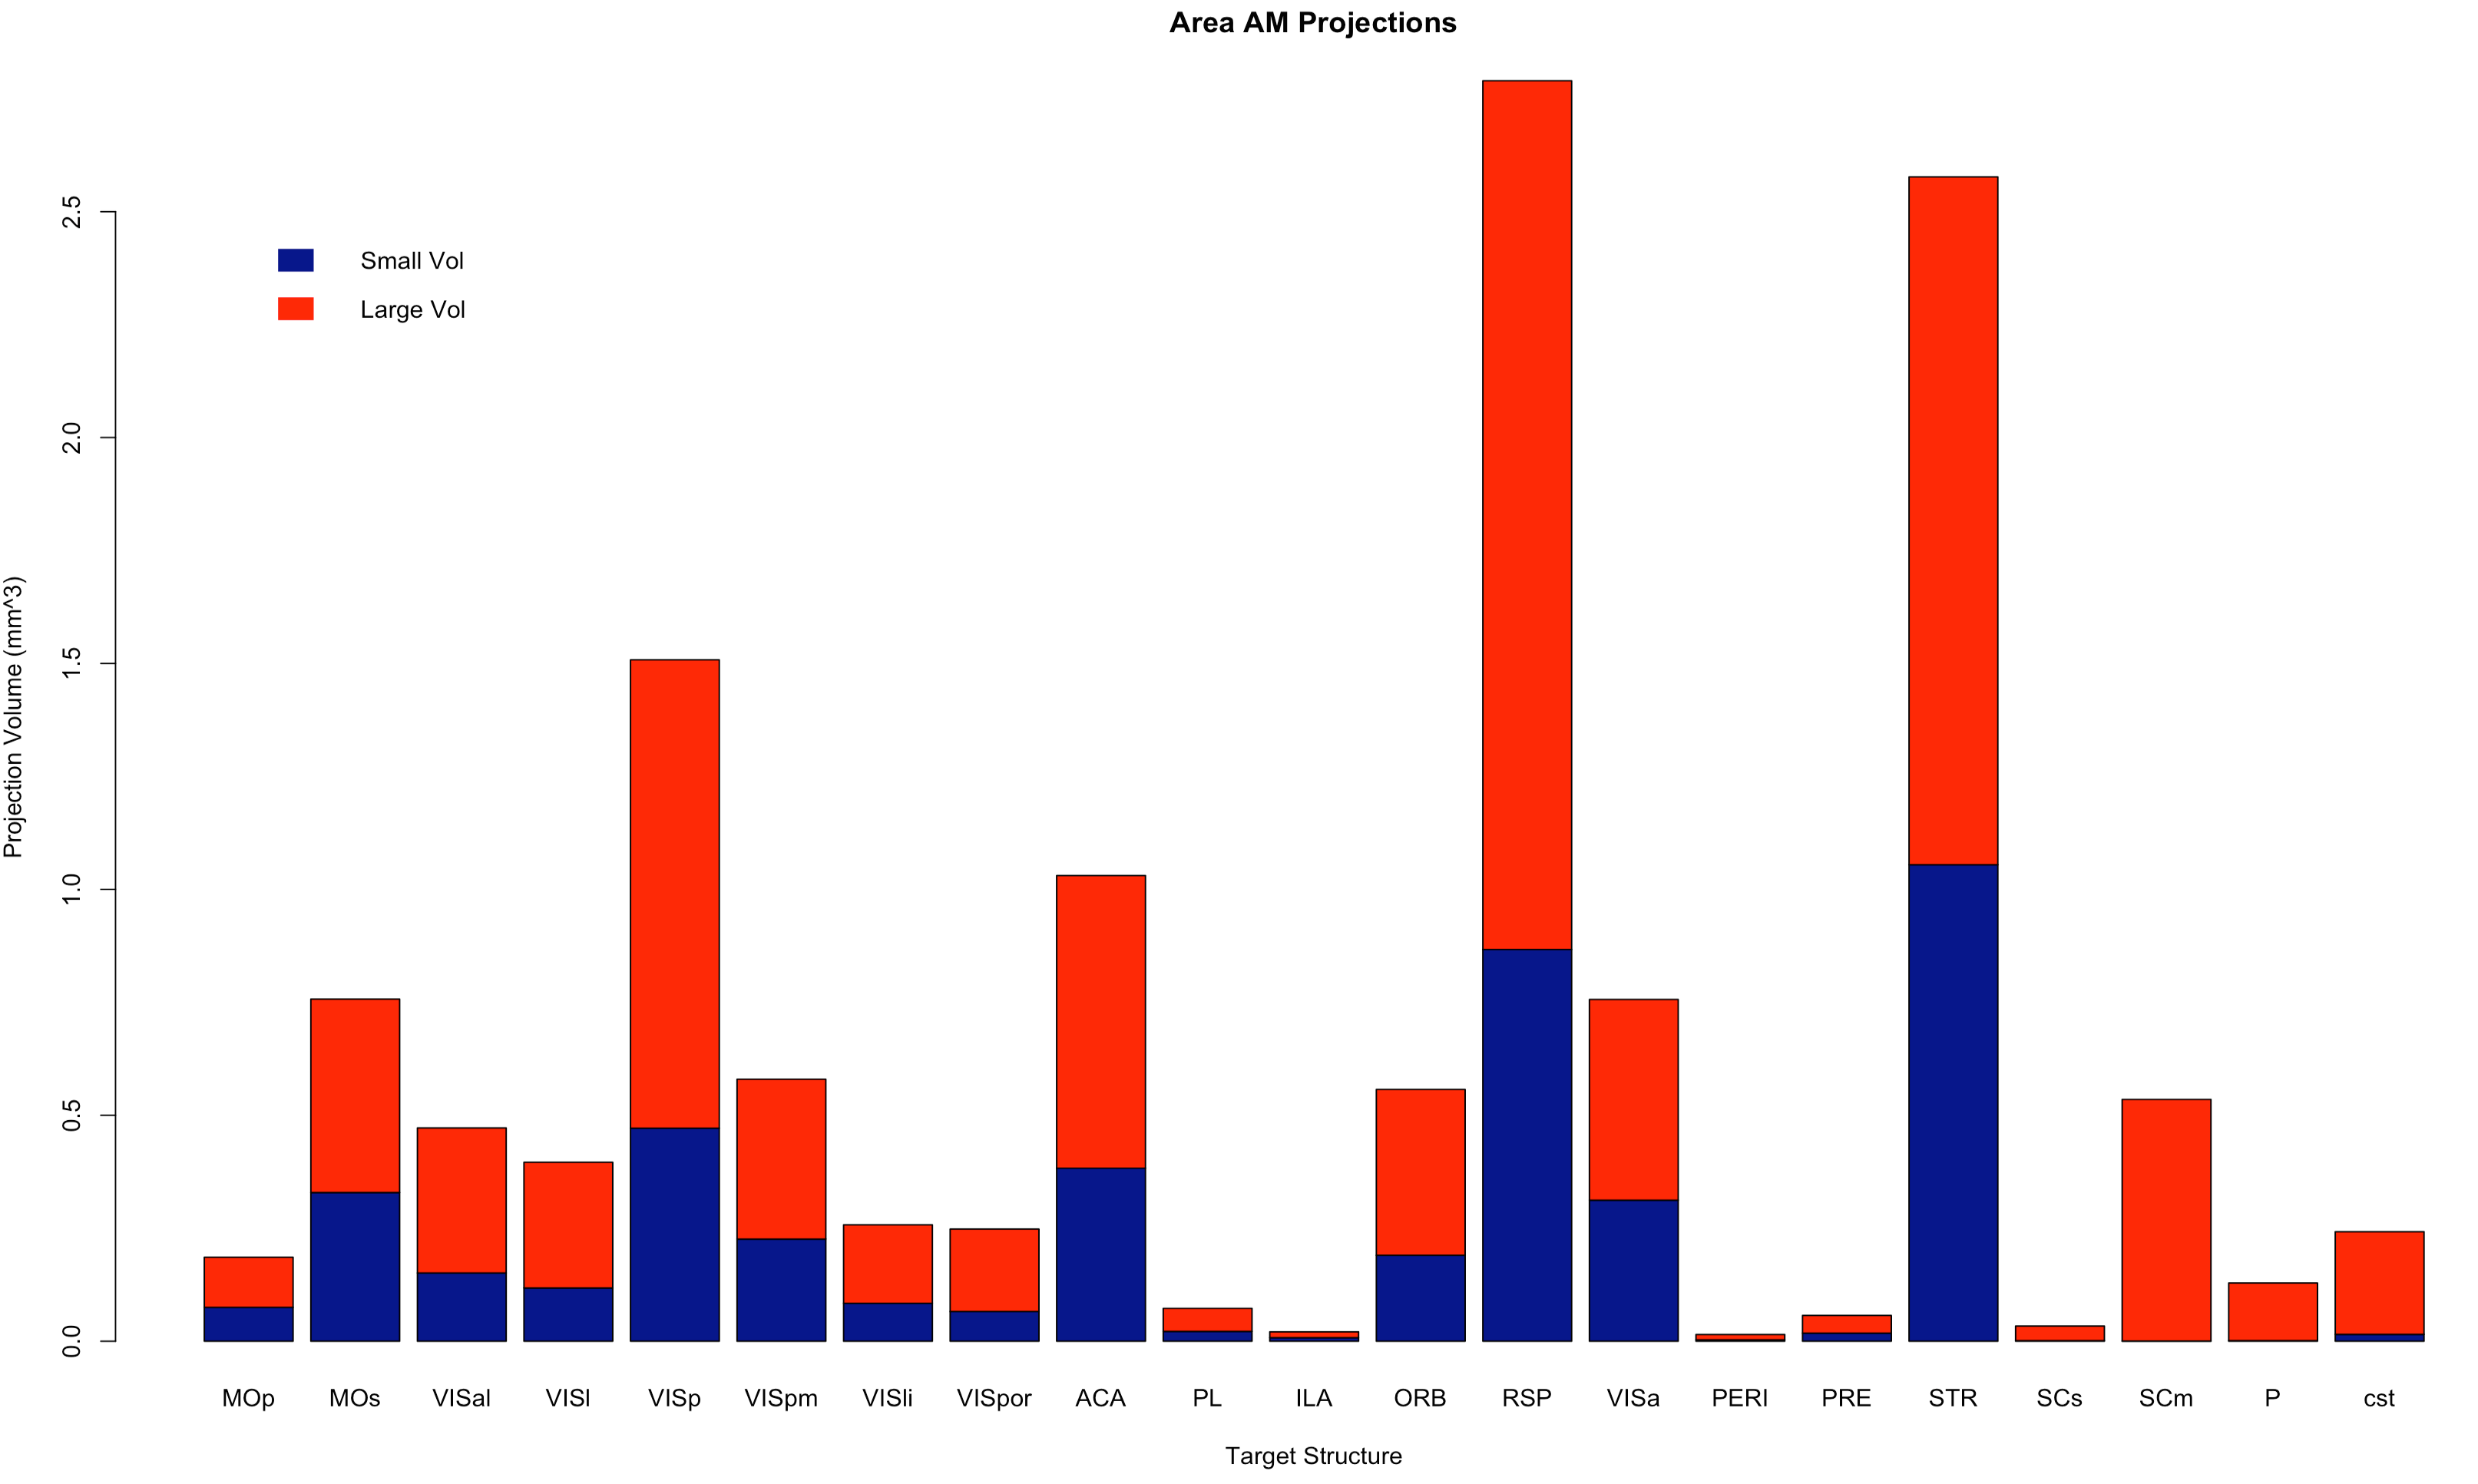
\includegraphics[width=\textwidth]{Figures/chapter4/areaAMprojectiondata2.png}
  \caption[Area AM Projection Target Data]{\textbf{Area AM Projection Target Data} Represented in a bar graph showing projection volume (sum of detected signal in mm\^3) at target structure for small (dark blue) and large (red) volume tracer injections. Data obtained from the Allen Institute Brain Connectivity Atlas \parencite{AllenBrain2015}; experiment id: 528510546 and 518742338.See list of abbreviations.}
   \label{fig:areaAMprojections}
\end{figure}

\section{General Experimental Strategy}
\subsection{Strategy for \emph{in vivo} optogenetic silencing of area AM}
The goal of the experiments in this chapter was to, reversibly, silence visual area AM as mice performed the visual pulses task. To this end, I employed an optogenetic strategy to silencing activity in area AM. Specifically, I used the cruxhalorhodopsin Jaws (or Halo57), a red light-driven chloride ion pump capable of powerful optogenetic inhibition \parencite{Chuong2014,Acker2016}. Another optogenetic approach that was explored in pilot experiments was to activate inhibitory neurons (PV+ or Gad2+)  optogenetic activator Channelrhodopsin (ChR2). Although cortical silencing through inhibitory neuron activation has been used to silence mouse visual cortex during behavior \parencite{Madisen2012,Glickfeld2013b,Poort2015,Burgess2016}, however this approach was incompatible with the widefield mapping of visual areas with GCaMP6 transgenic mice.\par
Details of the experimental procedures are described in Appendix \ref{AppendixA}. Briefly, area AM was identified in each mouse with widefield GCaMP6 imaging approach described in Chapter \ref{Chapter4}. Jaws was delivered into unilateral area AM through a viral construct with either a pan-neuronal promoter (human synapsin, hSyn, Group 1 mice) or excitatory neuron promoter (CamkII-$\alpha$, Group 2 mice). Optogenetic stimulation was randomly interleaved in 25\% of trials within a session. A linear downward ramp was added (Figure \ref{fig:AMgroup1summary} a) to the end of the optogenetic stimulus waveform to reduce the effect of rebound excitation that occurs during optogenetic inhibition \parencite{Chuong2014,Guo2014b}.
\begin{figure}
  \centering
   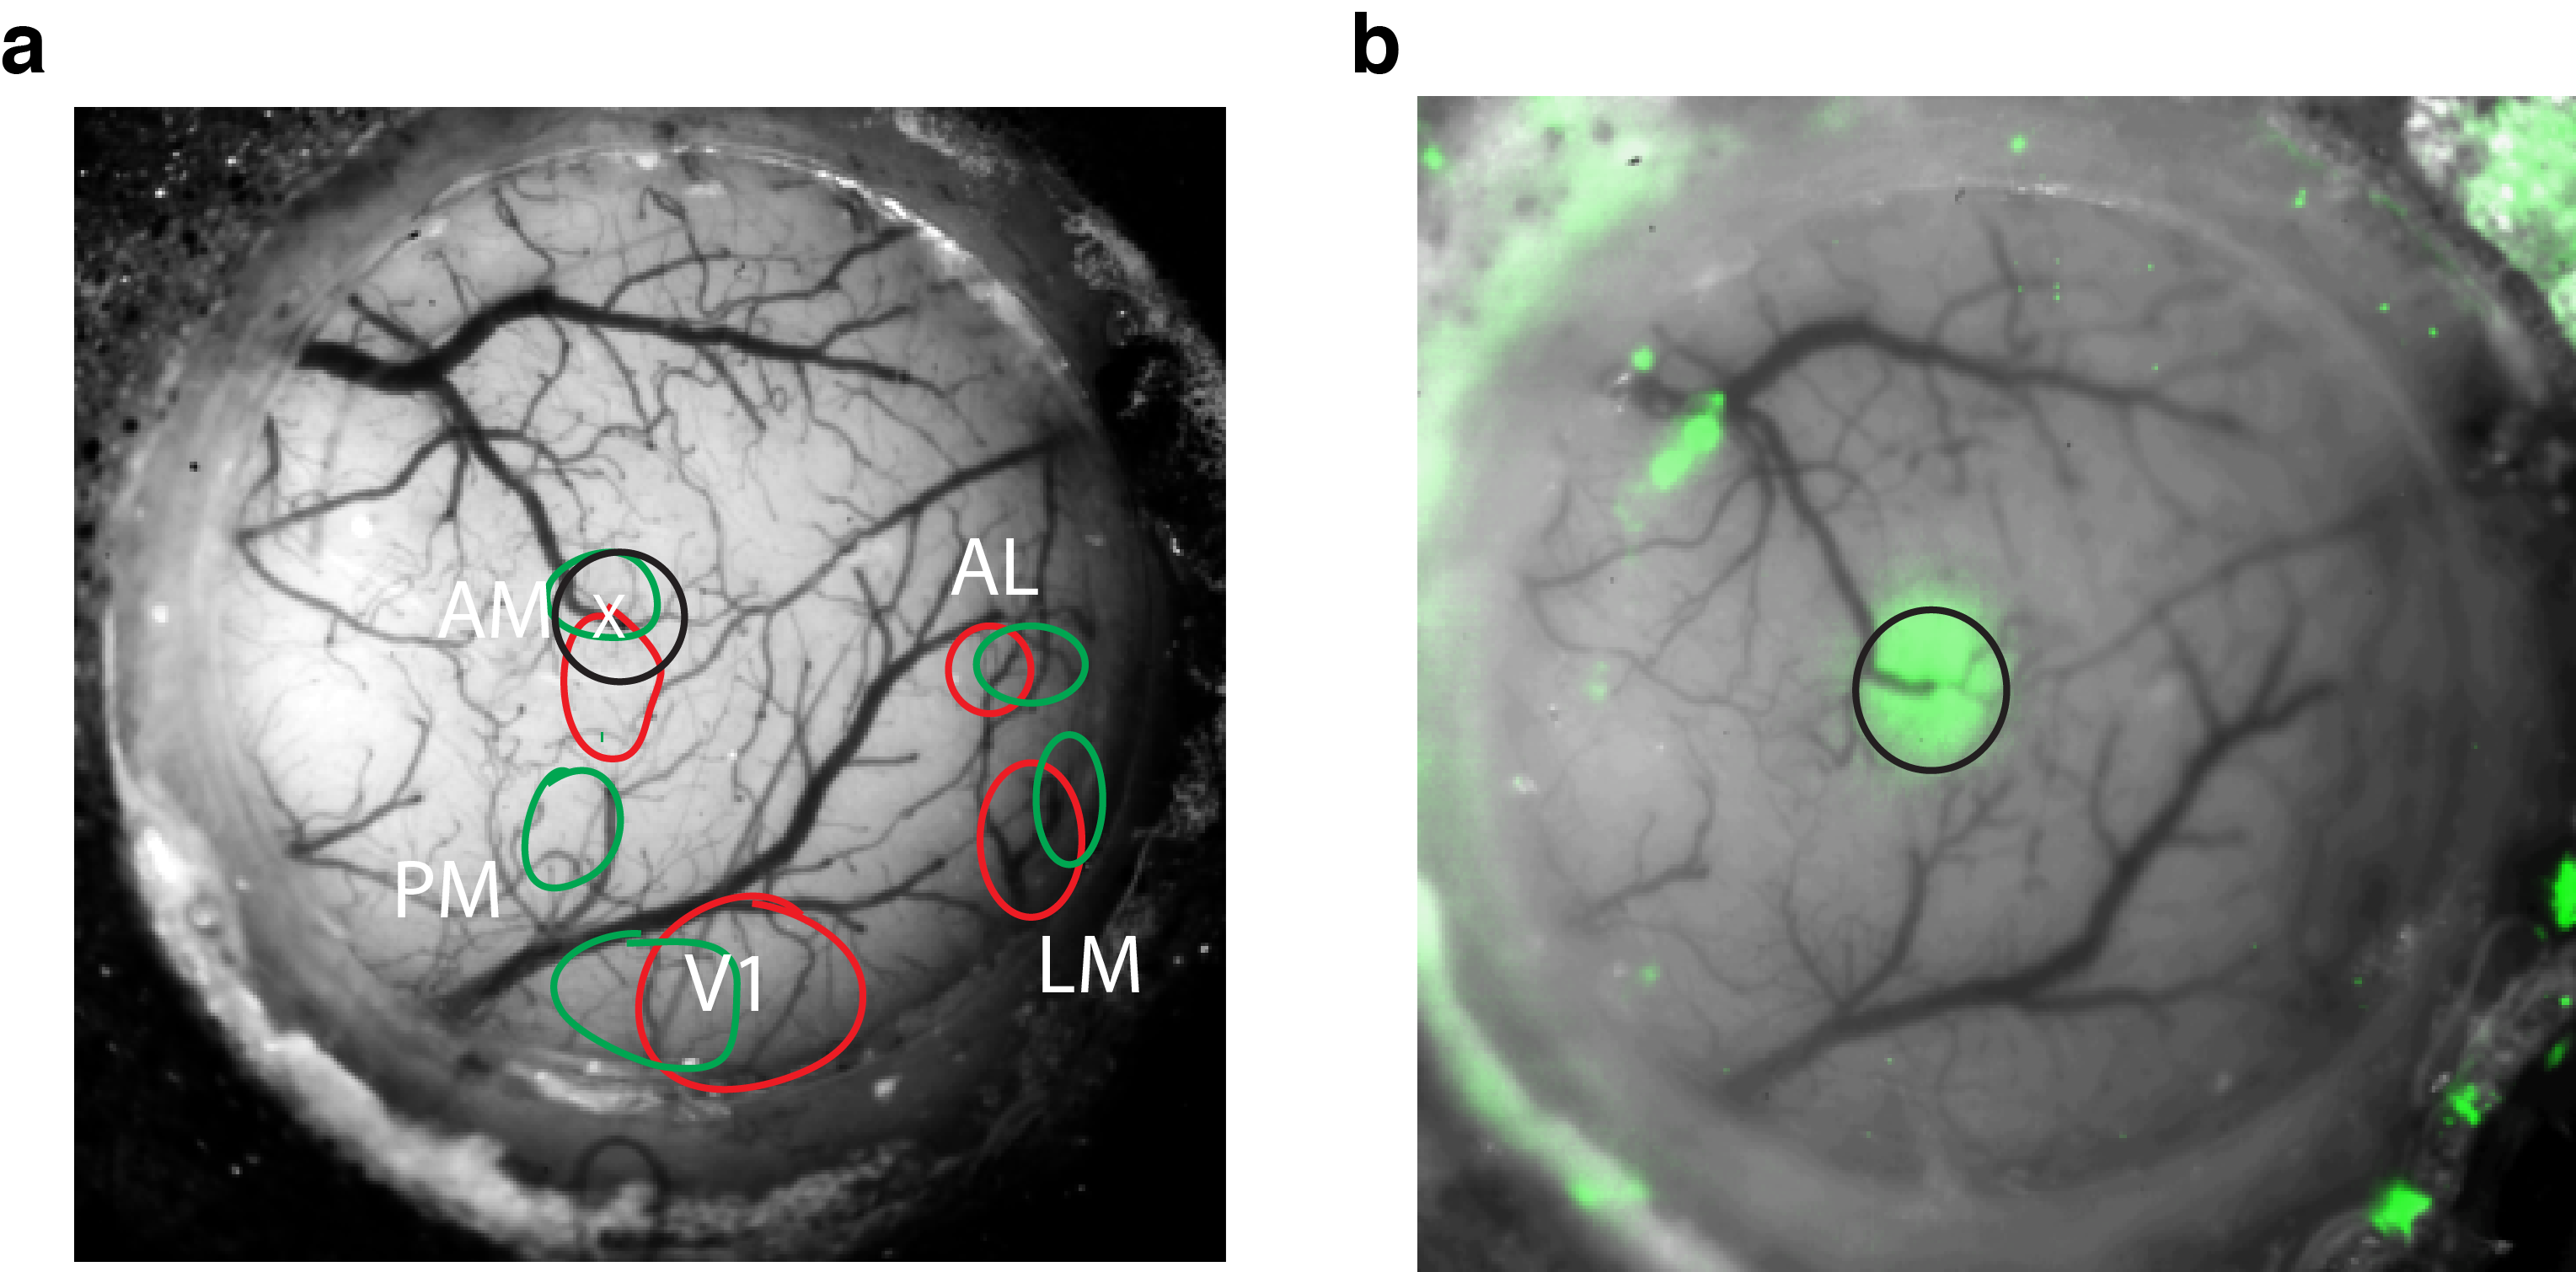
\includegraphics[width=\textwidth]{Figures/chapter4/kg07_jaws_gfp_expression.png}
  \caption[Jaws Virus Expression \emph{in vivo} in Area AM]{\textbf{Jaws Virus Expression \emph{in vivo} in area AM} (a) GCaMP6 response map overlay on optical window. Retinotopic map generated from response to drifting gratings (25$\deg$), 4Hz, 0.04 cycles/degree positioned at elevation of +15$\deg$ and azimuth 43$\deg$ (red) and 83$\deg$ (green). (b) Jaws-GFP expression (green) in area AM nine days post virus injection. }
   \label{fig:virusexp}
\end{figure}
%-----------------------------------------------------------------------
%------------------------------------------------------------------------
\subsection{Retinotopic Mapping of Visual Area AM}
Because of the small size of most visual areas including AM, their respective positions from bregma could vary from animal to animal; hence I performed retinotopic mapping in each mouse in order to target AM for viral delivery. To map visual areas, I imaged visually-evoked activity in awake transgenic mice expressing GCaMP6 in excitatory neurons (Ai95;Emx-cre and Ai93;ttA;Emx-cre) and generally employed one of two retinotopic mapping methods: spatially restricted gratings \parencite{Gias2005,Andermann2011} or periodic drifting bar \parencite{Sereno1995,Kalatsky2003}. The spatially-restricted gratings approach uses drifting gratings (25-40$\deg$ in diameter) positioned at different locations in the visual field (nasal vs. temporal or upper vs. lower). The gratings allow the experimenter to optimize the stimulus for the spatiotemporal frequency preferences of individual visual areas. Although this approach is easy to implement, in practice it requires many repetitions and high signal-to-noise to produce quality interpretable maps. The approach is not scalable because the maps need to be curated manually, and therefore not it was difficult to standardize across mice. Visual area AM was mapped using the grating procedure in a subset of mice (Figure \ref{fig:virusexp}, Group 1 below). \par 

I found the Fourier drifting bar methods to be a more consistent and scalable retinotopic mapping approach. Technical details and procedures for implementing the approach are described in \parencite{Kalatsky2003,Juavinett2016}. Briefly, a bar is periodically drifted across the screen in the 4 cardinal direction. Since the bar drifts at a fixed frequency, 
Fourier decomposition (Fast Fourier Transform) is used to isolate the phase at the bar drift (or stimulation) frequency. Phase maps are generated for the horizontal and vertical bar drift directions, which correspond to altitude and azimuth visual space (Figure \ref{fig:retinomap} a, b). Using a clever mathematical trick, visual field sign maps (Figure \ref{fig:retinomap}c) are generated by taking the sine of the difference between the gradients for the altitude and azimuth maps \parencite{Sereno1994,Garrett2014}. Borders between visual areas are defined With the visual field sign map (Figure \ref{fig:retinomap}d). I implemented this approach in awake head-fixed mice who were passively viewing the stimulus. The mice were free to walk on a wheel. \par 

\subsection{Statistical Analysis of Behavioral Performance}
The performance was visualized with the 4-parameter psychometric function described in Chapter \ref{Chapter2}. However, to statistically test whether there was a significant effect of photoinhibition of area AM on the population group level, I used a Generalized Linear Mixed-Model (GLMM). GLMMs are an extension of the Generalized Linear Model, which can be used to model both fixed and random effects in categorical data. In psychophysics, GLMMs can be used to generalize results across multiple subjects and experimental conditions \parencite{KnoblauchMaloney2012,Moscatelli2012a,Erlich2015}. \\The GLMM model written in the Wilkinson notation:
\begin{equation}
	\centering
	r \sim  1 + evidence + opto + evidence:opto + (evidence|subject/opto)
    \label{GLMM}
\end{equation}
Each term of the equation has a coefficient, $\beta$. The model specifies that the subject's response, \emph{r}, is a function of the fixed effects: intercept, the \emph{evidence} which represents the slope of the psychometric function is defined as the difference between the flash rate and the category boundary, the photoinhibition indicator variable \emph{opto}, and the interaction between the \emph{evidence} and \emph{opto}. The interaction term \emph{evidence:opto} evaluates whether photoinhibition alters the subject's sensitivity or the slope of the psychometric function. The model allows the four fixed effects parameters to vary for each individual subject (random effects). The model uses a probit linking function and was fit using a Maximum Likelihood procedure. The GLMM analysis was performed using the R package 'lme4' and is identical to the analysis used by \textcite{Erlich2015}. \par 

The effect of photoinhibition on the horizontal location of the psychometric function was quantified by the choice bias (Figure \ref{fig:amGLMMparams}b). The choice bias was defined as: 
\begin{equation}
	\centering
	choice\quad bias =  \frac{\beta_{opto}}{\beta_{evidence}+\beta_{evidence:opto}}
    \label{choicebias}
\end{equation}
Where $\beta_{opto}$, $\beta_{evidence}$, $\beta_{evidence:opto}$ are estimated coefficients from the GLMM (Equation \ref{GLMM}). The choice bias reflects the equivalent change in the stimulus that would recapitulate the observed effects of photoinhibition and is in units of flashes/s. Positive choice bias would indicate that on photoinhibition trials caused the subject to be biased towards high-rate responses. Because the choice bias is computed from estimated parameters of the GLMM model, I used error propagation to compute the errors (95\% confidence intervals, CI).

%----------------------------------------------------------------------------------
\begin{figure}
  \centering
   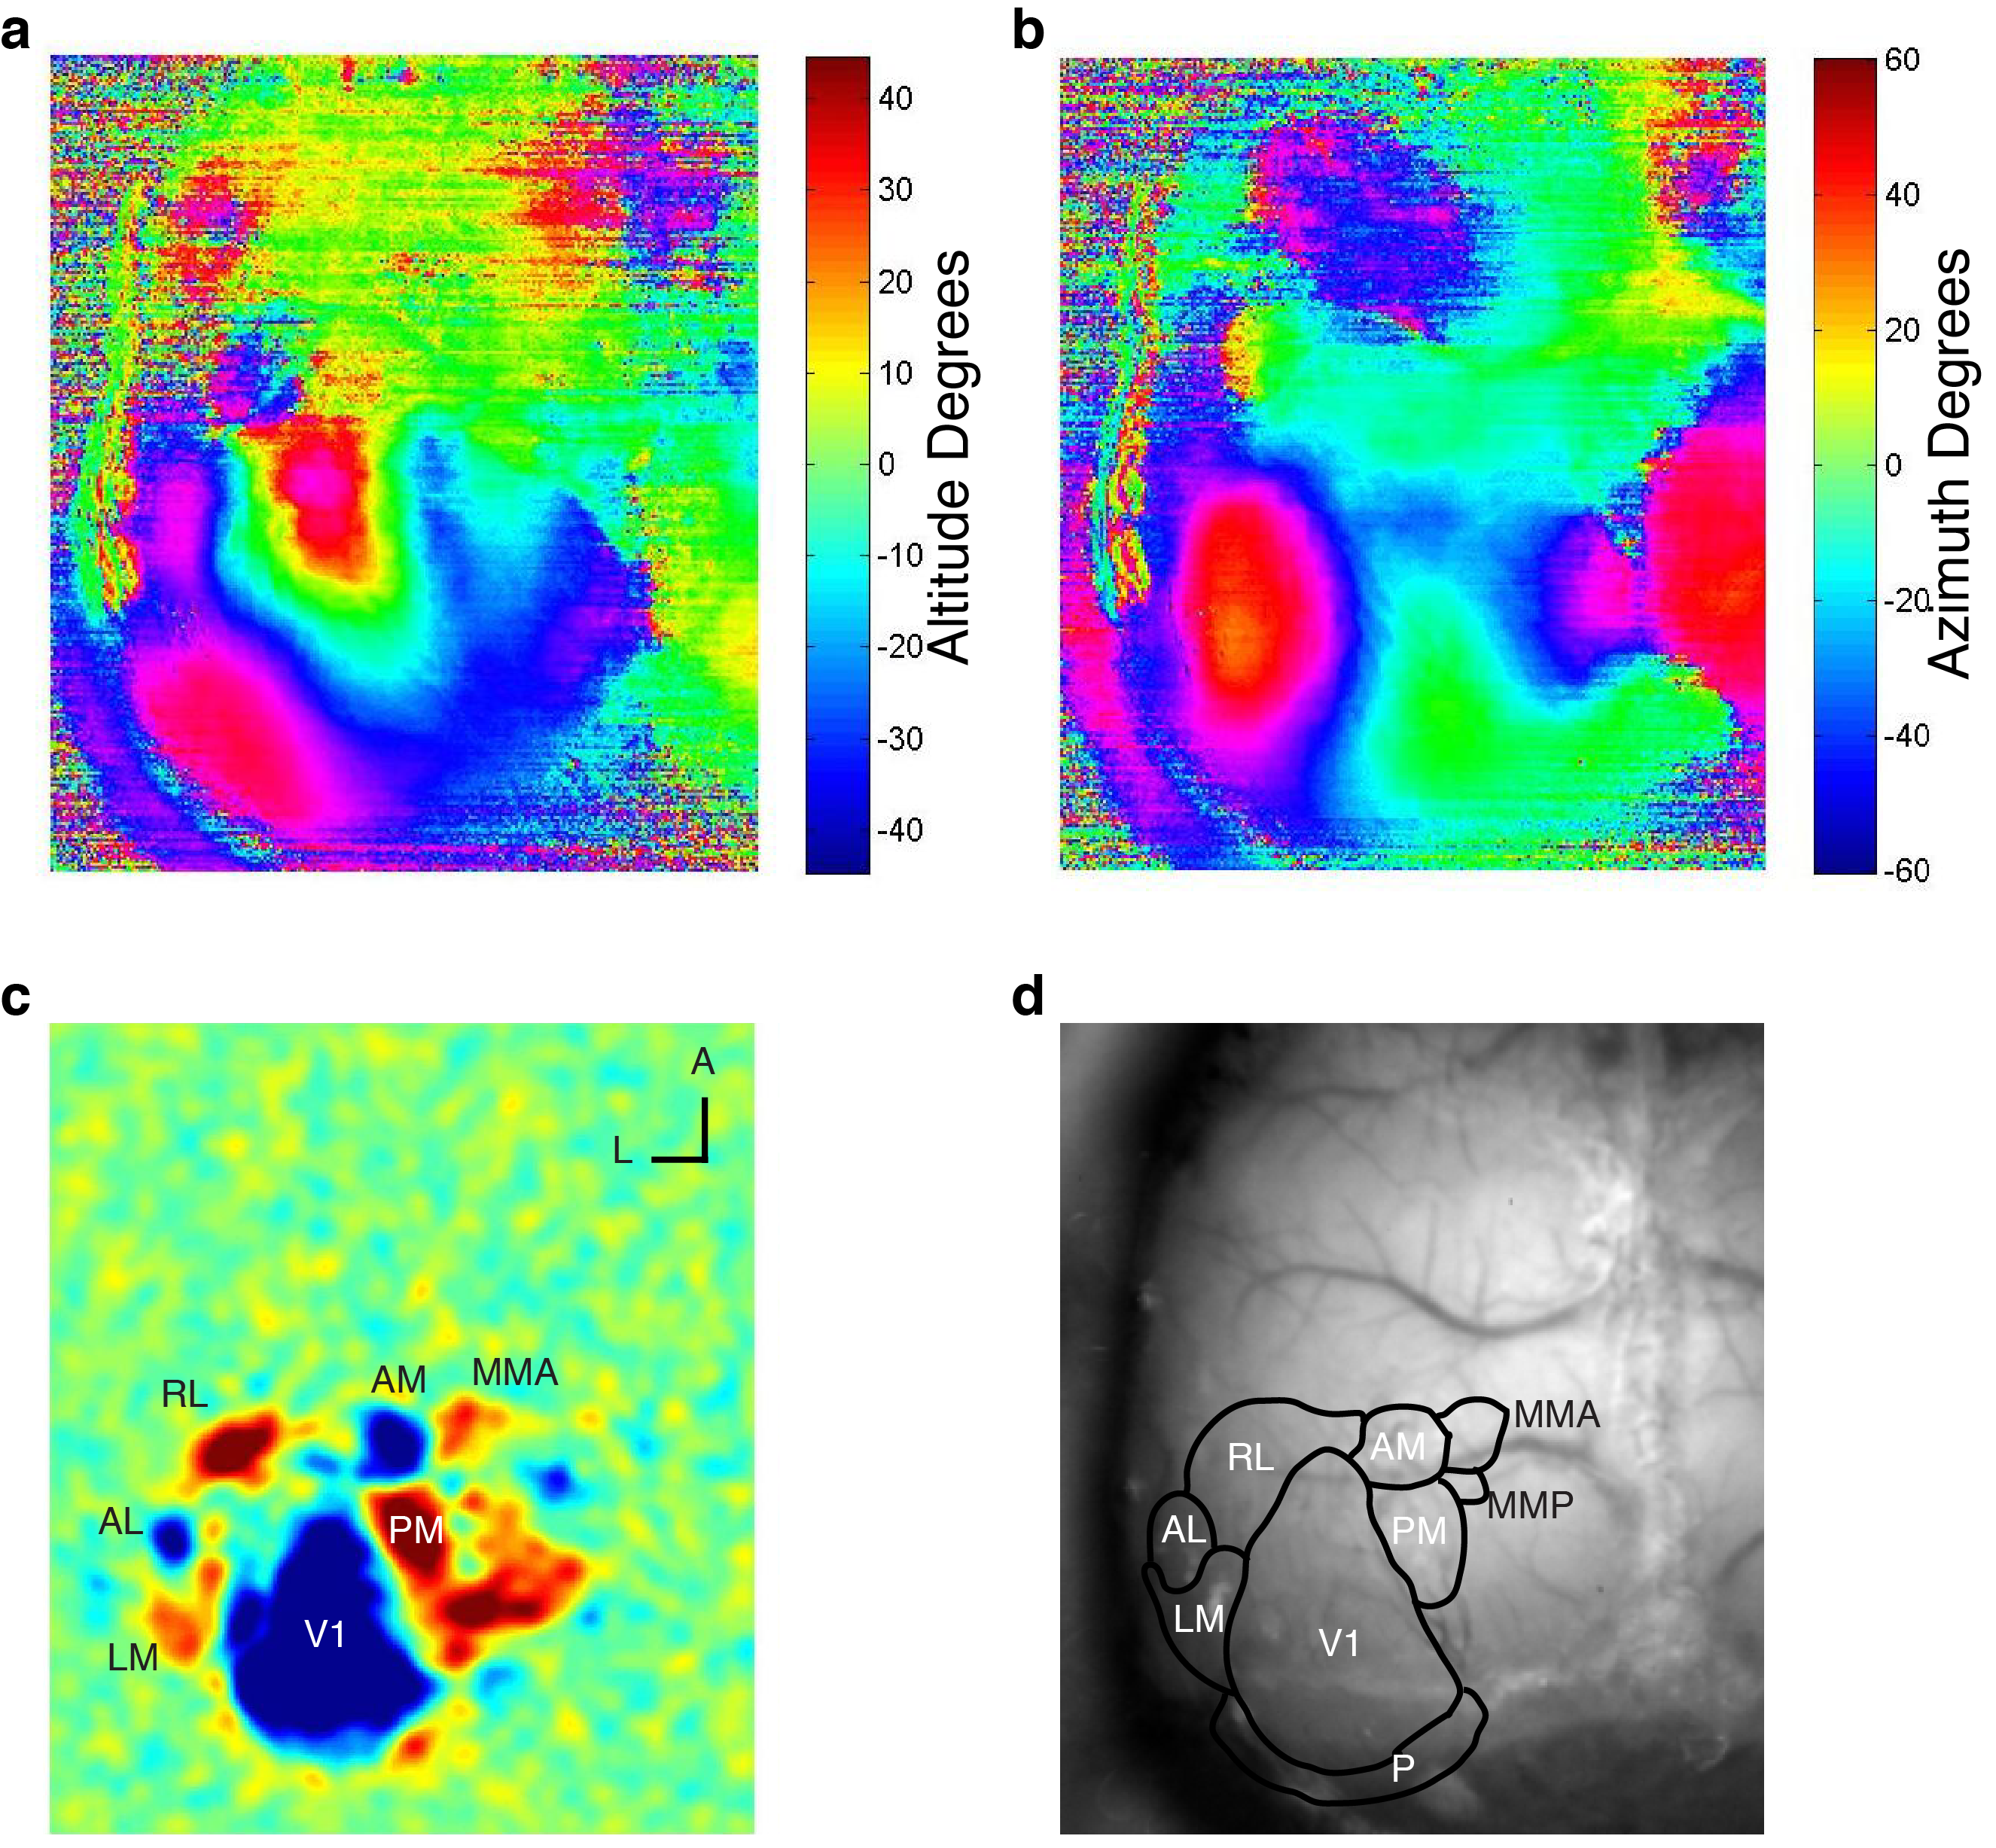
\includegraphics[width=\textwidth]{Figures/chapter4/retino_maps.png}
  \caption[Example Retinotopic Map of Mouse Visual Areas]{\textbf{Example Retinotopic Map of Mouse Visual Areas}. (a) Altitude and (b) Azimuth phase map (c) Visual field sign map with labeled visual areas (d) Overlay of visual areas borders on skull. Borders drawn by hand with visual field sign map.}
   \label{fig:retinomap}
\end{figure}
%---------------------------------------------------------------------------
%-------------------------------------------------------------------------------
\section{Predicted Consequences of Unilateral Inhibition of Visual Area AM}
Since the behavioral consequences of inhibiting mouse secondary visual areas are largely unknown, let us consider the potential behavioral outcomes of optogenetic inhibition of area AM (Figure \ref{fig:predictions}). Several outcomes are possible including, (a) a shift in choice bias, (b) a change in sensitivity, (c) a combination of changes in sensitivity and bias, or (d) no effect. 

Photoinhibition of AM could cause a horizontal shift in the psychometric function (Figure \ref{fig:predictions}a), which would indicate either a sensory bias towards a stimulus category (i.e. low- or high-rate) or a spatial bias towards a response port (i.e. left or right-hand port). A sensory bias could occur if AM selectively preferred low- or high-rate stimuli. This is an attractive viewpoint given that higher-order visual areas in the mouse have distinct preferences for temporal frequency \parencite{Andermann2011,Marshel2011,Tohmi2014}. However, it is not clear whether these preferences extend to stochastic (i.e. non-periodic) sequences of flashes and more so, how visual areas represent the visual pulses stimuli remains an open question. Alternatively, AM is in a position to mediate a spatial bias. It is reciprocally connected with cortical \parencite{Wang2012} and subcortical motor areas \parencite{AllenBrain2015} (Figure \ref{fig:areaAMprojections}), which are capable of biasing movements. Recently, \textcite{Znamenskiy2013b} showed that manipulation of corticostriatal projections in rat selectively biased choices in an auditory evidence accumulation task. 

Photoinhibition of AM could reduce sensitivity (Figure \ref{fig:predictions}b). Since area AM is a retinotopic visual area, it could also be involved in the processing of the visual flashes stimulus in a manner that informs computation of the choice downstream. Therefore inhibition of area AM could affect the slope of the psychometric curve, i.e. the subject's sensitivity. Reduced sensitivity would be consistent with results presented in the previous chapter (Chapter \ref{Chapter3}), and previous studies in rat PPC \parencite{Raposo2014,Licata2017}. 

While manipulation of AM could produce shifts in sensitivity and/or changes in bias, the manipulation may also have no behavioral consequence o
in the visual pulses task either because the neural activity in area AM does not contribute to the behavior or because unilateral silencing is not sufficient to disrupt the behavior. In the latter case, the opposite hemisphere is still intact and may compensate for the loss of unilateral activity \parencite{Li2016}. The scenario is plausible since the animals are presented with full- field visual flashes and presumably, information comes in to both eyes and, by extension, both hemispheres of AM.

%-----------------------------------------------------------------------------
\begin{figure}
  \centering
   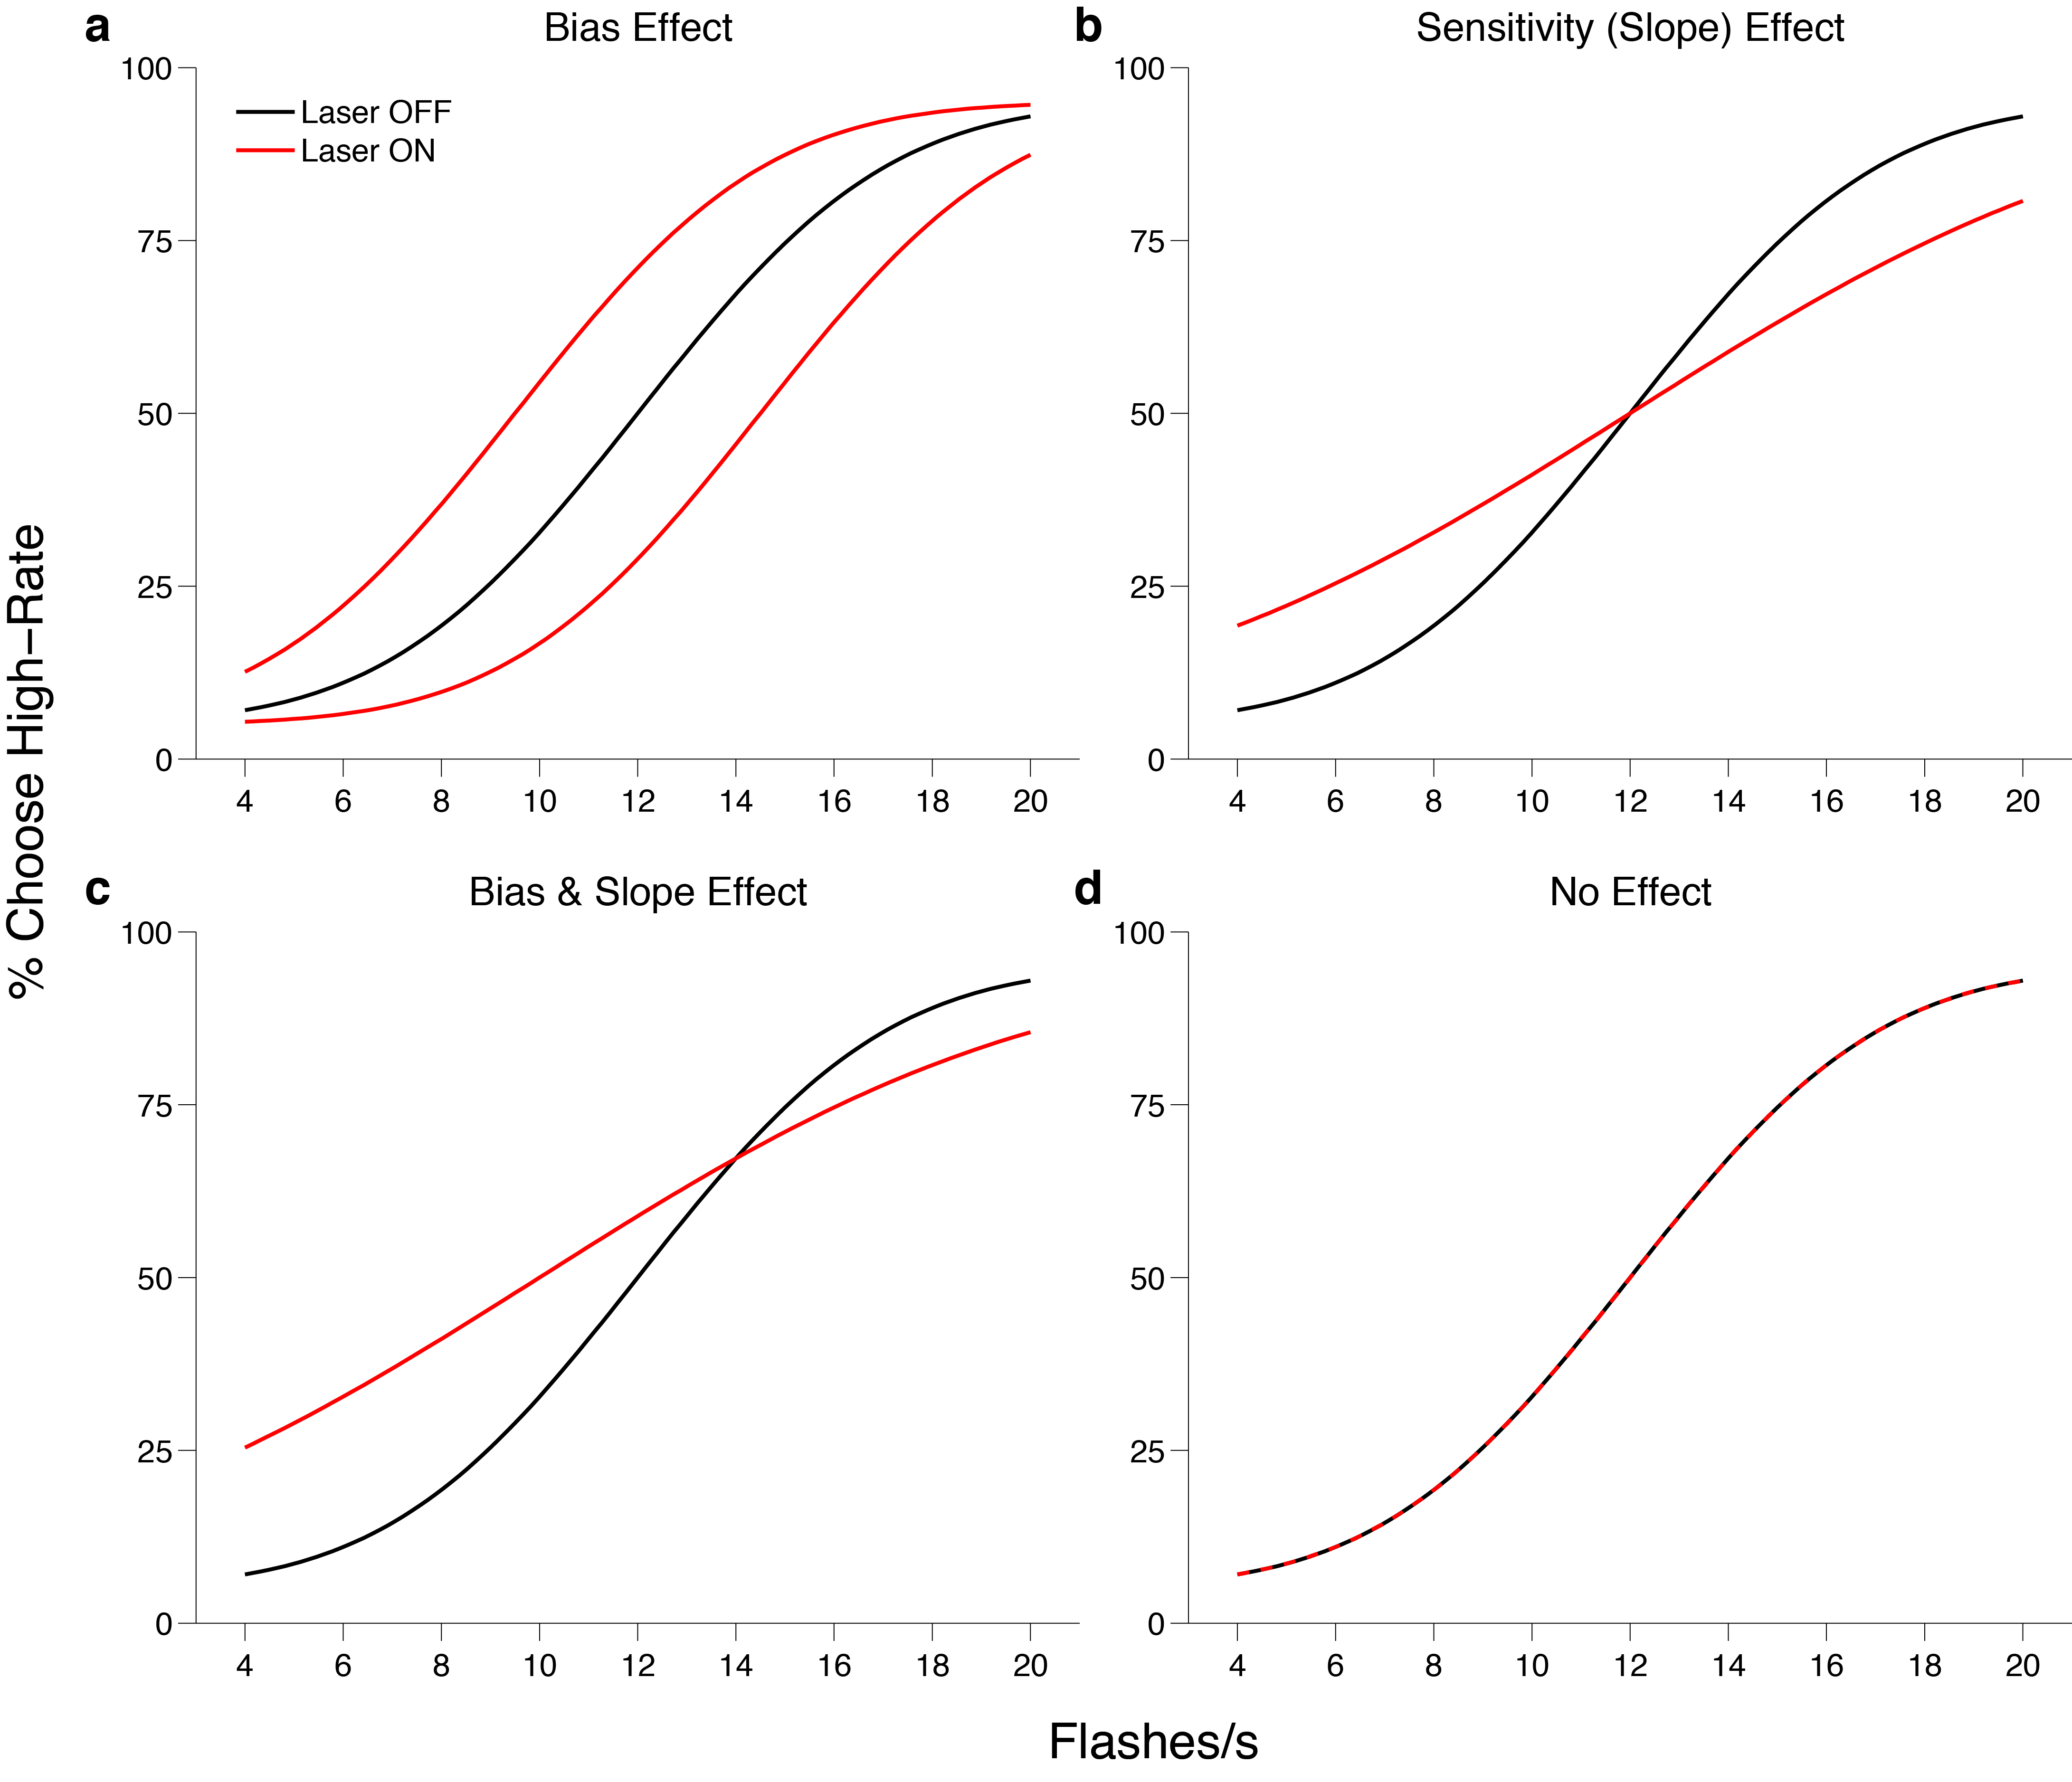
\includegraphics[width=\textwidth]{Figures/chapter4/pmfPredictions.png}
  \caption[Schematic of Potential Behavioral Outcomes of Optogenetic Inhibition]{\textbf{Schematic of Potential Behavioral Outcomes of Optogenetic Inhibition} Optogenetic inhibition of visual area AM could potentially cause: (a) horizontal shift in the psychometric function, (b) change in slope i.e. sensitivity, (c) both shift in bias and change in sensitivity, or (d) no effect.}
   \label{fig:predictions}
\end{figure}
%-----------------------------------------------------------------------------
\section{Results}
\subsection{Area AM Inhibition - Group 1}
The first group of mice (Figures \ref{fig:AMgroup1summary}, \ref{fig:AMgroup1individual}, and \ref{fig:AMg1GLMM32}, n = 6 mice, Ai95;Emx-cre) were injected with Jaws in the right hemisphere and were trained with the standard contingency (Low-rate go LEFT and High-rate go RIGHT). Photoinhibition occurred randomly on 25\% of trials, at an irradiance of 32 mW/mm$^{2}$. On laser ON trials, all mice in this group exhibited an increased tendency to make more high-rate choices (Figures \ref{fig:AMgroup1summary}, \ref{fig:AMgroup1individual}, and \ref{fig:AMg1GLMM32}), as indicated by a leftward shift of the psychometric function on photoinhibition trials (red) compared to control trials (black). The observed bias had the equivalent effect of adding more flashes (choice bias = 3.47 flashes/s [2.46 4.54] 95\% CI), as quantified by Equation \ref{choicebias}. AM photoinhibition also caused a significant decrease in the animals' sensitivity, as indicated by a decrease in the slope of the psychometric function on Laser ON trials (GLMM Test, $\beta_{evidence:opto}$ = -0.021 [-0.034, -0.0085] 95\% CI, p=0.0011). The change is equivalent to a 16.58\% reduction in the slope on Laser ON compared to Laser OFF trials. The combined effect of the horizontal shift and reduced sensitivity is consistent the predictions made in Figure \ref{fig:predictions}c and in line with the anatomical and functional properties of AM. Therefore the results thus far lend support for the role of visual area AM in visually-guided decision making. \par 

The observed bias could be a result of either a sensory, high-rate, bias or a spatial bias towards the ipsilateral hemifield in the direction of the optogenetic stimulation site. Therefore, based on this experiment alone the animals could have either a sensory (perceptual) bias towards high rate stimuli or a spatial (or motor) bias towards the right hemifield, ipsilateral to the implanted site. Plausible experiments that could disentangle these two hypotheses include (A) photoinhibition of the opposite hemisphere under the same behavioral contingency (Low-rate, go LEFT and High-Rate, go RIGHT) or (B) photoinhibition of the same hemisphere and and a reversed behavioral contingency (Low-rate, go RIGHT and High-Rate, go LEFT).\par

%-----------------------------------------------------------------------------
\begin{figure}
  \centering
   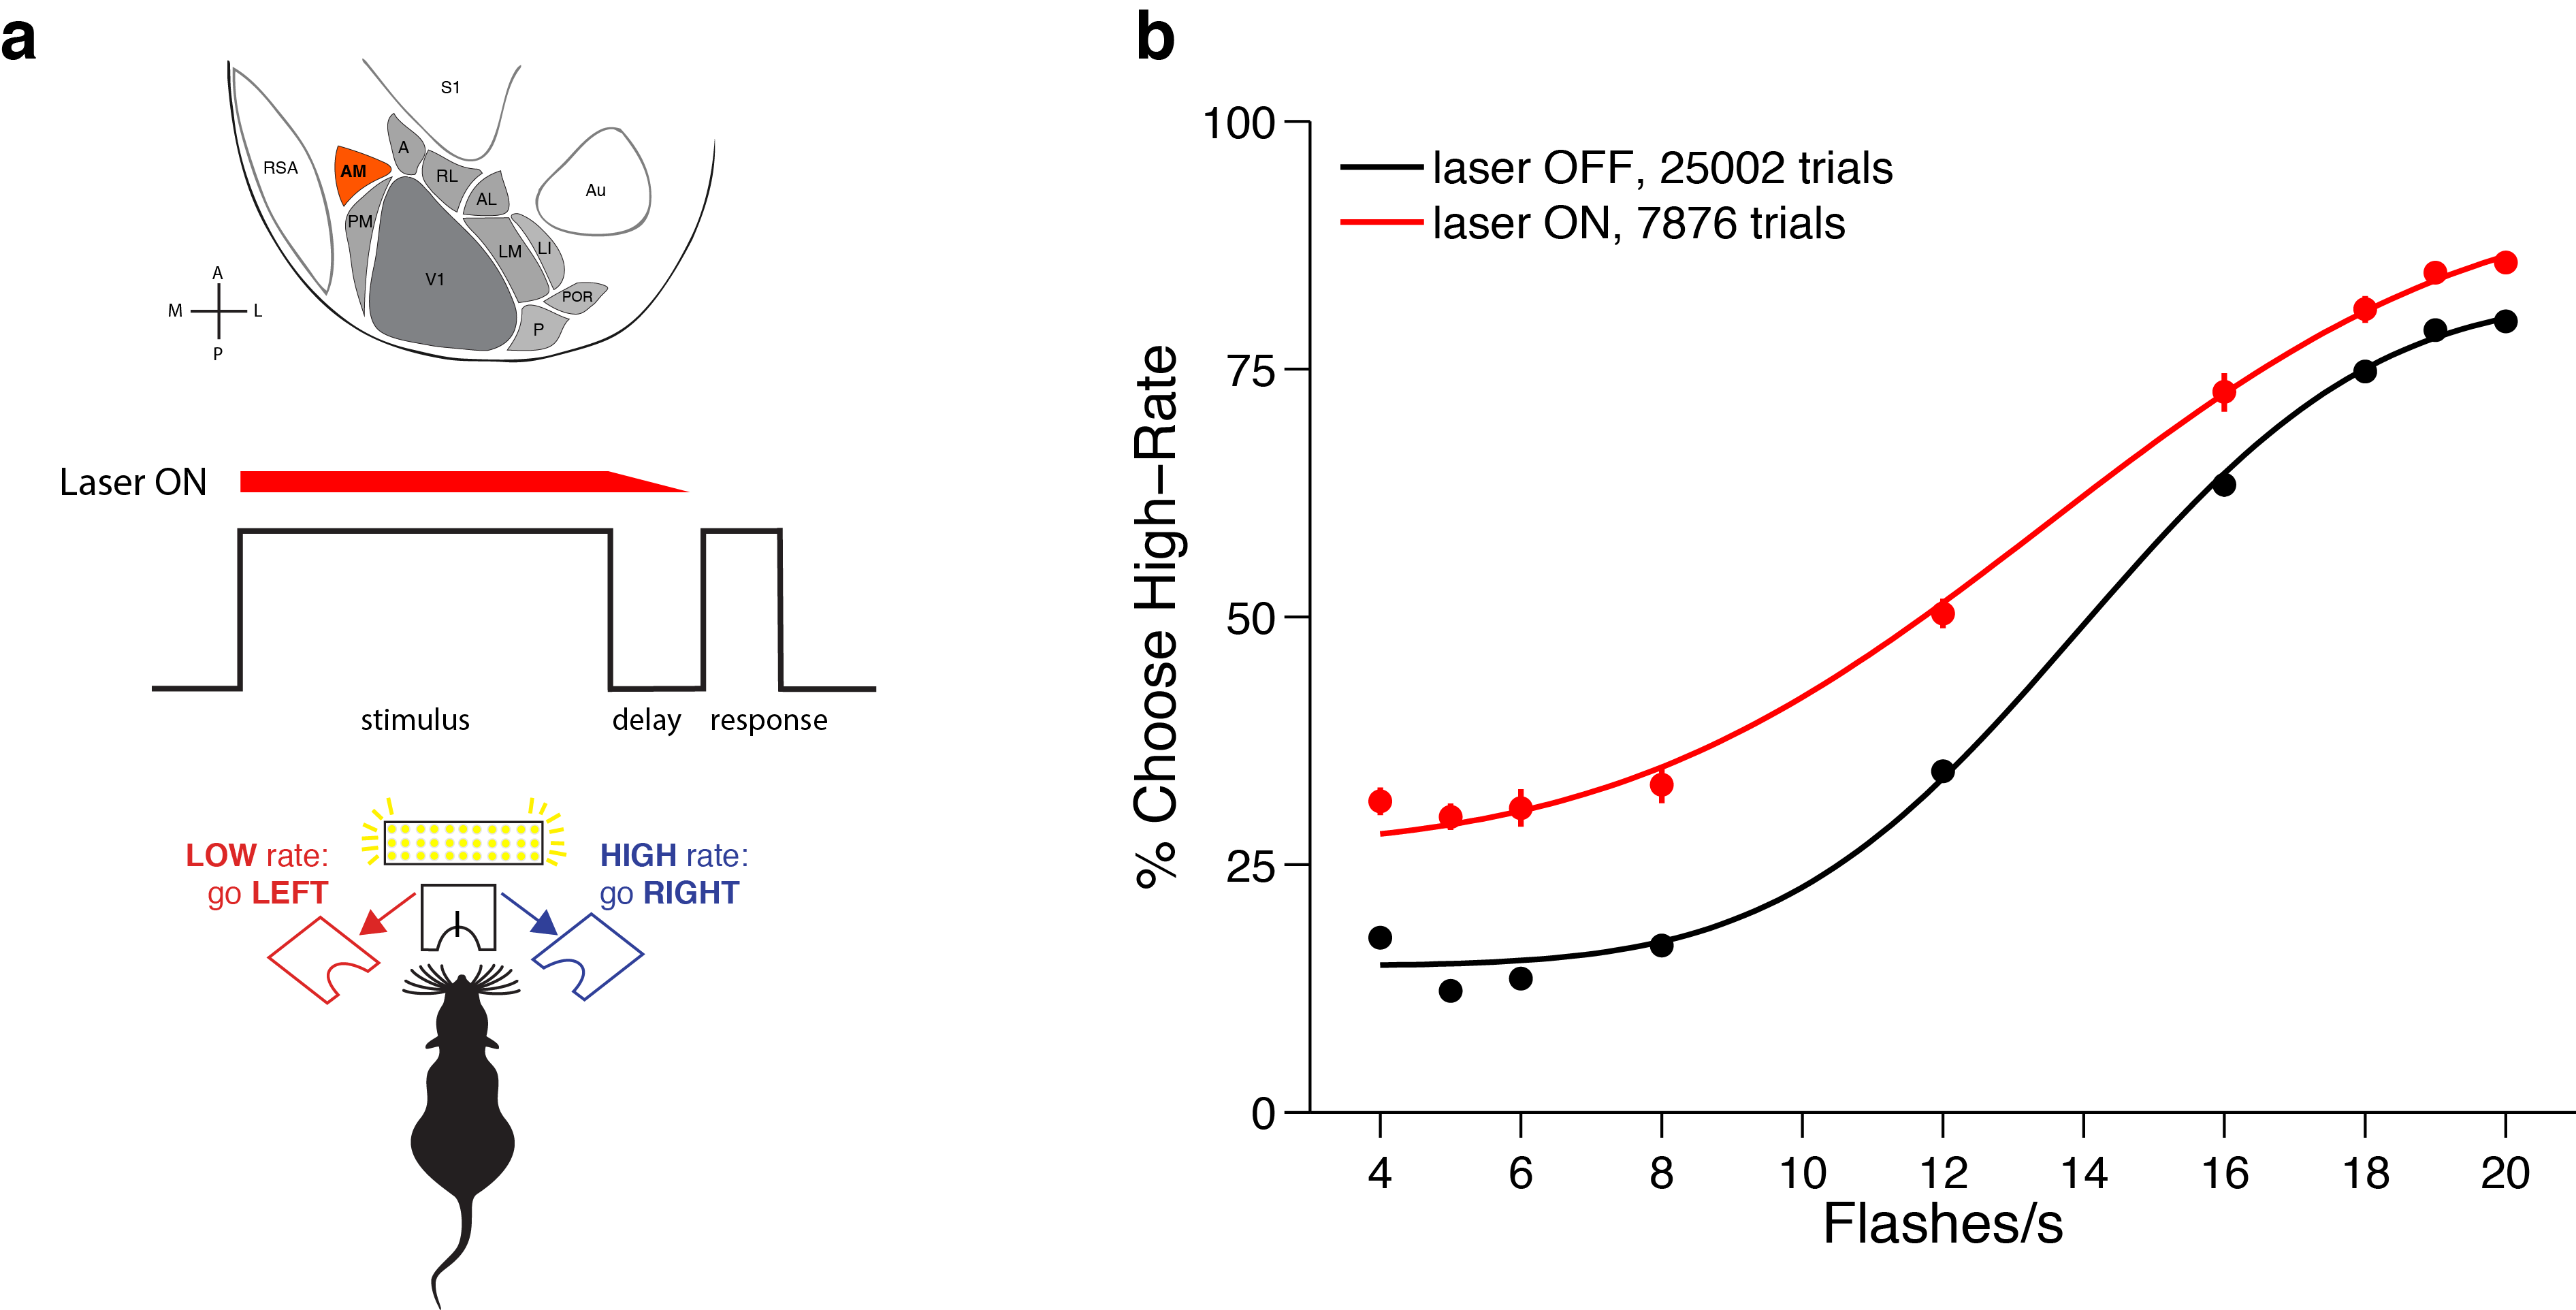
\includegraphics[width=\textwidth]{Figures/chapter4/jaws_AM_group1_summaryPMF.png}
  \caption[Area AM Group 1 Summary Psychophysical Data]{\textbf{Area AM Group 1 Summary Psychophysical Data} (a) Schematic of experimental configuration for group 1 animals.(b) Psychometric data of mice (n = 6) on laser OFF (black) and laser ON (red) trials (irradiance at 32 mW/mm$^{2}$). Circles represent psychometric performance at each event rate and the solid line is the psychometric function fit with a cumulative Normal (Equation \ref{eq:normalpmf}). Errors bars represent Wilson binomial confidence intervals on the psychometric data.}
   \label{fig:AMgroup1summary}
\end{figure}

%-----------------------------------------------------------------------------
%-----------------------------------------------------------------------------
\subsection{\emph{In Vivo} Red Light Stimulation Control Group}
The observation that inhibition of area AM increased the tendency to make high-rate choices could potentially explained by an artifact of the red light optogenetic stimulation, such that the mice are biased towards the red light delivered through the unilateral implanted optical fiber. Compared to short wavelength light such as blue and green, red light scatters minimally in tissue and is therefore able to travel several millimeters from the fiber implant site through the mouse's eyes \parencite{Danskin2015}.\par

To test whether this artifact contributed to behavioral effects observed in Group 1, I repeated the experiment in a new group of mice that were not injected with Jaws. Instead, the mice were injected with a sham virus (AAV-GFP) in area AM and implanted with an optical fiber. If the red light stimulation alone has no effect on the behavior, there would be no difference in the psychometric function (Figure \ref{fig:predictions} d; however, if the red light stimulation alone causes an artifact such as light directly activating the retina from within the brain \parencite{Danskin2015}, then the change in the psychometric curve would be similar to that observed in Group 1. \par

\emph{In vivo} red light stimulation of the control group resulted in behavioral effects (Figures \ref{fig:ctrlsummary} a and \ref{fig:ctrlindividual} a,c) similar to group 1. This observation is consistent with the idea that the red light alone introduces an artifact in the behavior, possibly due to red light escaping through eyes. However, the observed behavioral artifact in the controls does not rule out the possibility that unilateral inhibition of area AM inhibition does not have an effect on the behavior as observed in group 1 mice. The solution proposed by  \textcite{Danskin2015} to eliminate the behavioral artifact caused by \emph{in vivo} red light stimulation was to adapt the retina with dim white light near the eyes. However, application of this solution was maladaptive on the visual pulses task, as it reduced the subject's overall sensitivity and performance on the visual pulses task. \par

A solution that did not interfere with the subject's performance was to install red light within the behavior booth (Figure \ref{fig:mousehouselight} b). The external house red lights served to mask the red light escaping through the eyes and implant margins (Figure \ref{fig:mousehouselight} a), thereby making the mice less sensitive to the perception of red light. The artifact caused by \emph{in vivo} red light stimulation was greatly reduced by the presence of the house red lights (Figure \ref{fig:ctrlsummary}b, \ref{fig:ctrlindividual} b,d, and \ref{fig:glmmcontrol}), although it did not completely eliminate the artifact when the mice were again tested with more flash rates (Figures \ref{fig:ctrlpmfs}). 
%-----------------------------------------------------------------------------
\begin{figure}
  \centering
   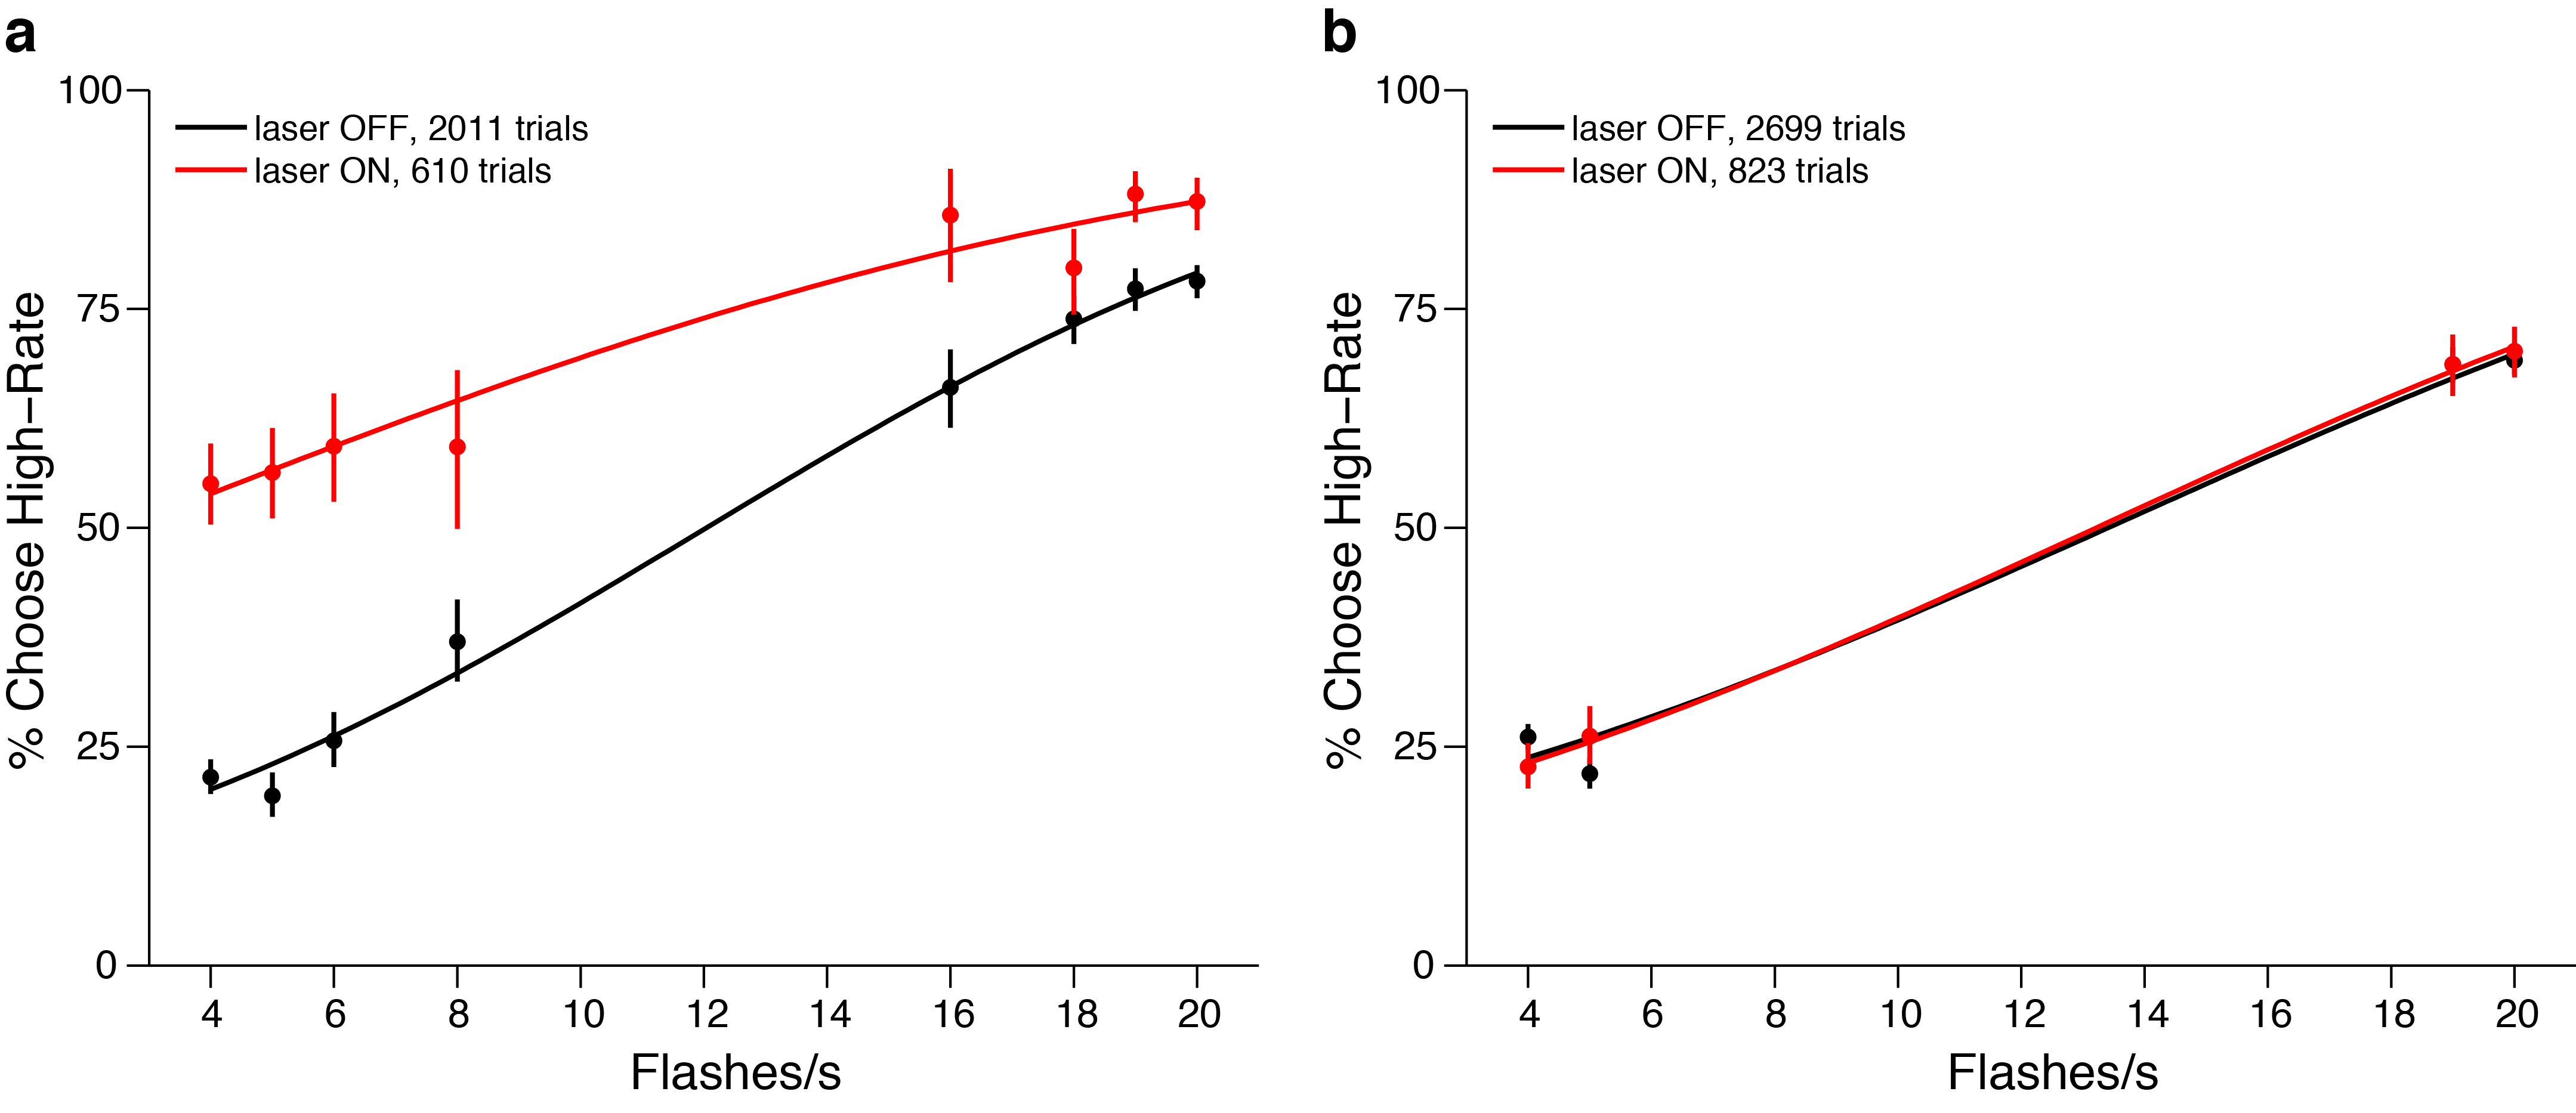
\includegraphics[width=\textwidth]{Figures/chapter4/jaws_controls_summaryPMFs.png}
  \caption[Control Group Summary Psychophysical Data ]{\textbf{Control Group Summary Psychophysical Data} (a) Under identical conditions as Group 1 (ie. no masking red light). Irradiance at 32mW/mm$^{2}$. (b) Masking red light installed in the behavior booth. Irradiance at 64mW/mm$^{2}$. Circles represent the subject's behavioral response during laser OFF (black) and laser ON (red) trials. Solid line represents the psychometric function fit to cumulative Normal (Equation \ref{eq:normalpmf}). Error bars represent Wilson Binomial (95\%) confidence intervals. }
   \label{fig:ctrlsummary}
\end{figure}

\begin{figure}
  \centering
   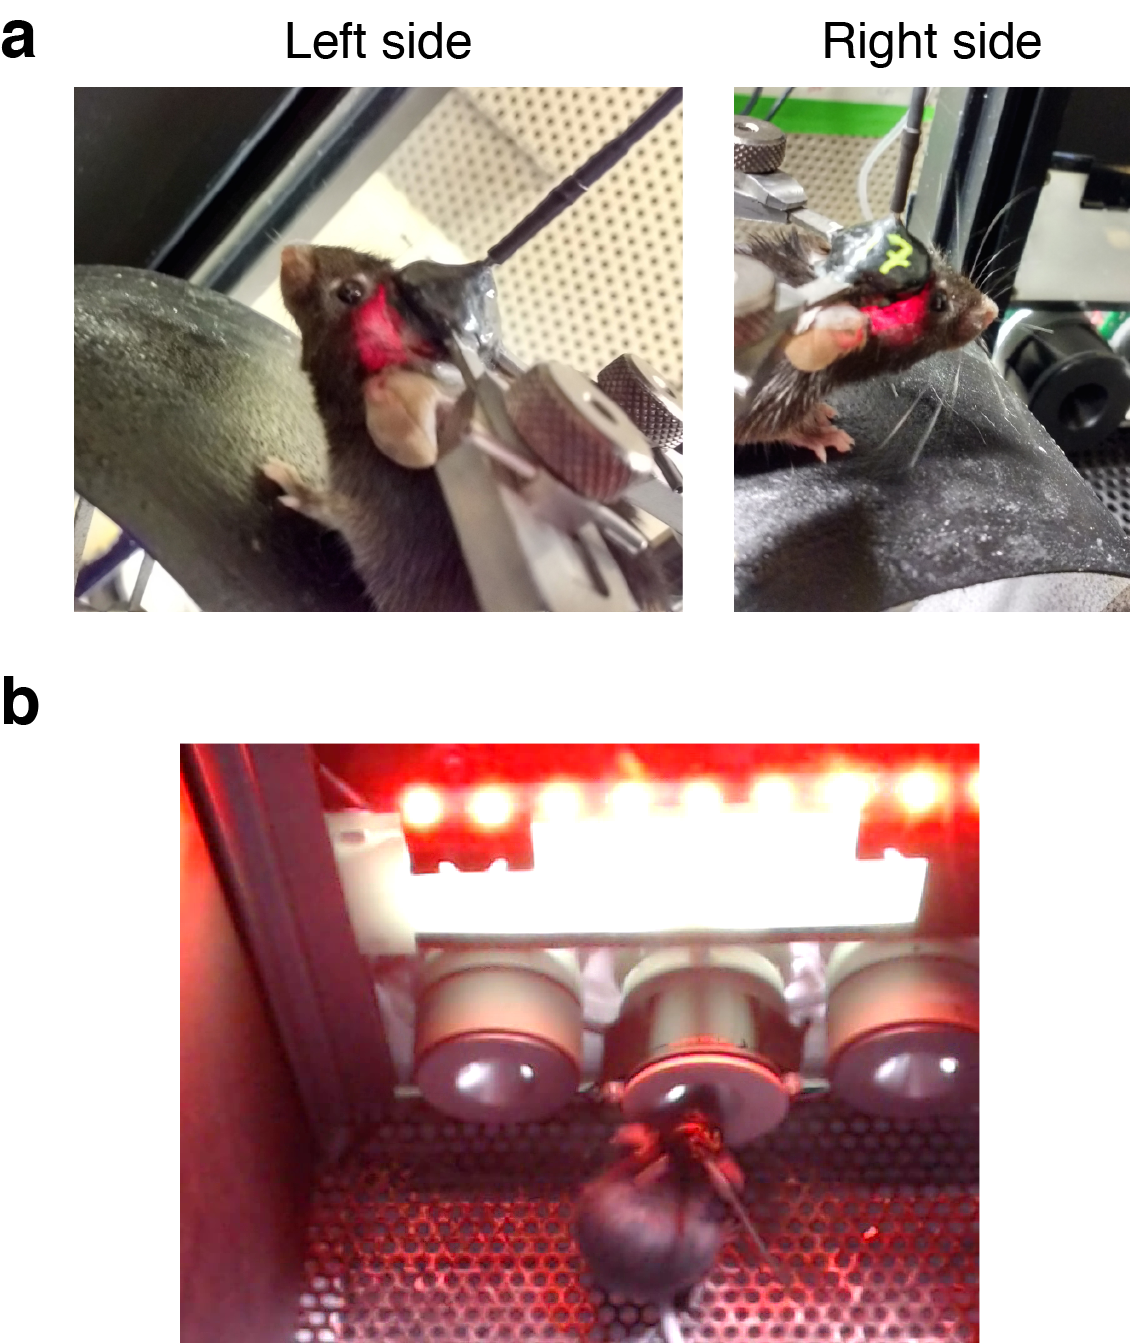
\includegraphics[width=\textwidth]{Figures/chapter4/mouse_house_red_light.png}
  \caption[\emph{In Vivo} Red Light Stimulation and House Red Lights]{\textbf{\emph{In Vivo} Red Light Stimulation and House Red Lights} (a) Left and right side view of mouse implanted with optical fiber with red light \emph{in vivo} illumination at irradiance of 32mW/mm$^{2}$. (b) Mouse in booth with house (masking) red light.}
   \label{fig:mousehouselight}
\end{figure}
%-----------------------------------------------------------------------------
%-----------------------------------------------------------------------------
\subsection{Area AM Inhibition - Group 2}
To distinguish whether the behavioral effects observed in Group 1 (Figure \ref{fig:AMgroup1summary}) were due to a sensory stimulus or spatial/motor bias, and to reduce the artifact caused by \emph{in vivo} red light stimulation, I repeated the area AM inhibition experiments in a new cohort of animals (n = 8 animals, Ai93;ttA;Emx-cre). The cohort of mice (Group 2) were injected with Jaws and implanted with an optical fiber in visual area AM on the left hemisphere. For behavior, they were split into two groups with one group (2A) running on the standard contingency (High-Rate, go RIGHT; Figure \ref{fig:AMgroup2schem} a) and the second group (2B) running on the reverse contingency (High-Rate, go LEFT; Figure \ref{fig:AMgroup2schem}b). Both groups of mice performed the task with the masking red lights to reduce the red light artifact.\par

The results from these two groups of mice make testable predictions that would disentangle whether the observed bias behavioral impact of area AM photoinhibition is sensory or spatial-motor in nature. For example, in the standard behavioral contingency, if the effect of AM photoinhibition is a sensory bias, then inhibition of area AM in both groups should cause a leftward shift in the psychometric function to indicate a bias towards the high-rate port. This would imply opposing spatial motor biases, where Group 2A would exhibit a contralateral bias away from and Group 2B an ipsilateral bias towards the implanted site. However, if inhibition of area AM causes a spatial (motor) bias towards the ipsilateral hemifield, then the psychometric function would shift in the opposing directions for the two groups. Group 2A would exhibit a rightward shift and Group 2B a leftward in the psychometric function. \par 

The psychophysical performance of Group 2 mice was impaired by photoinhibition of area AM (Figure \ref{fig:AMgroup2summary}). Although the behavioral impact on Group 2A and 2B were similar, group 2B (reverse contingency) exhibited pronounced deficits in performance across multiple laser power (irradiance) levels. In Figure \ref{fig:amGLMMparams}a the effect of photoinhibition on the animals' sensitivity ($\beta_{evidence:opto}$) is plotted as function of photoinhibition strength (irradiance, mW/mm$^{2}$). Photoinhibition significantly reduced the slope of the psychometric functions for subjects in Group 2B at irradiance levels 32 mW/mm$^{2}$ (p = 7.2e$^{-05}$) and 64 mW/mm$^{2}$ (p = 3.4e$^{-06}$). The sensitivity of Group 2A subjects was affected only at 32 mW/mm$^{2}$ (p = 7.3e$^{-06}$). Individual psychometric functions fitted to GLMM are shown in Figures \ref{fig:amGLMM16},\ref{fig:amGLMM32}, and \ref{fig:amGLMM64}. \par 

If the both groups of animals experienced a sensory high-rate bias, then the choice biases of both groups should increase with photoinhibition strength. This relationship was only observed in Group 2B, but not in Group 2A mice (Figure \ref{fig:amGLMMparams}b). \par 

\begin{figure}
  \centering
   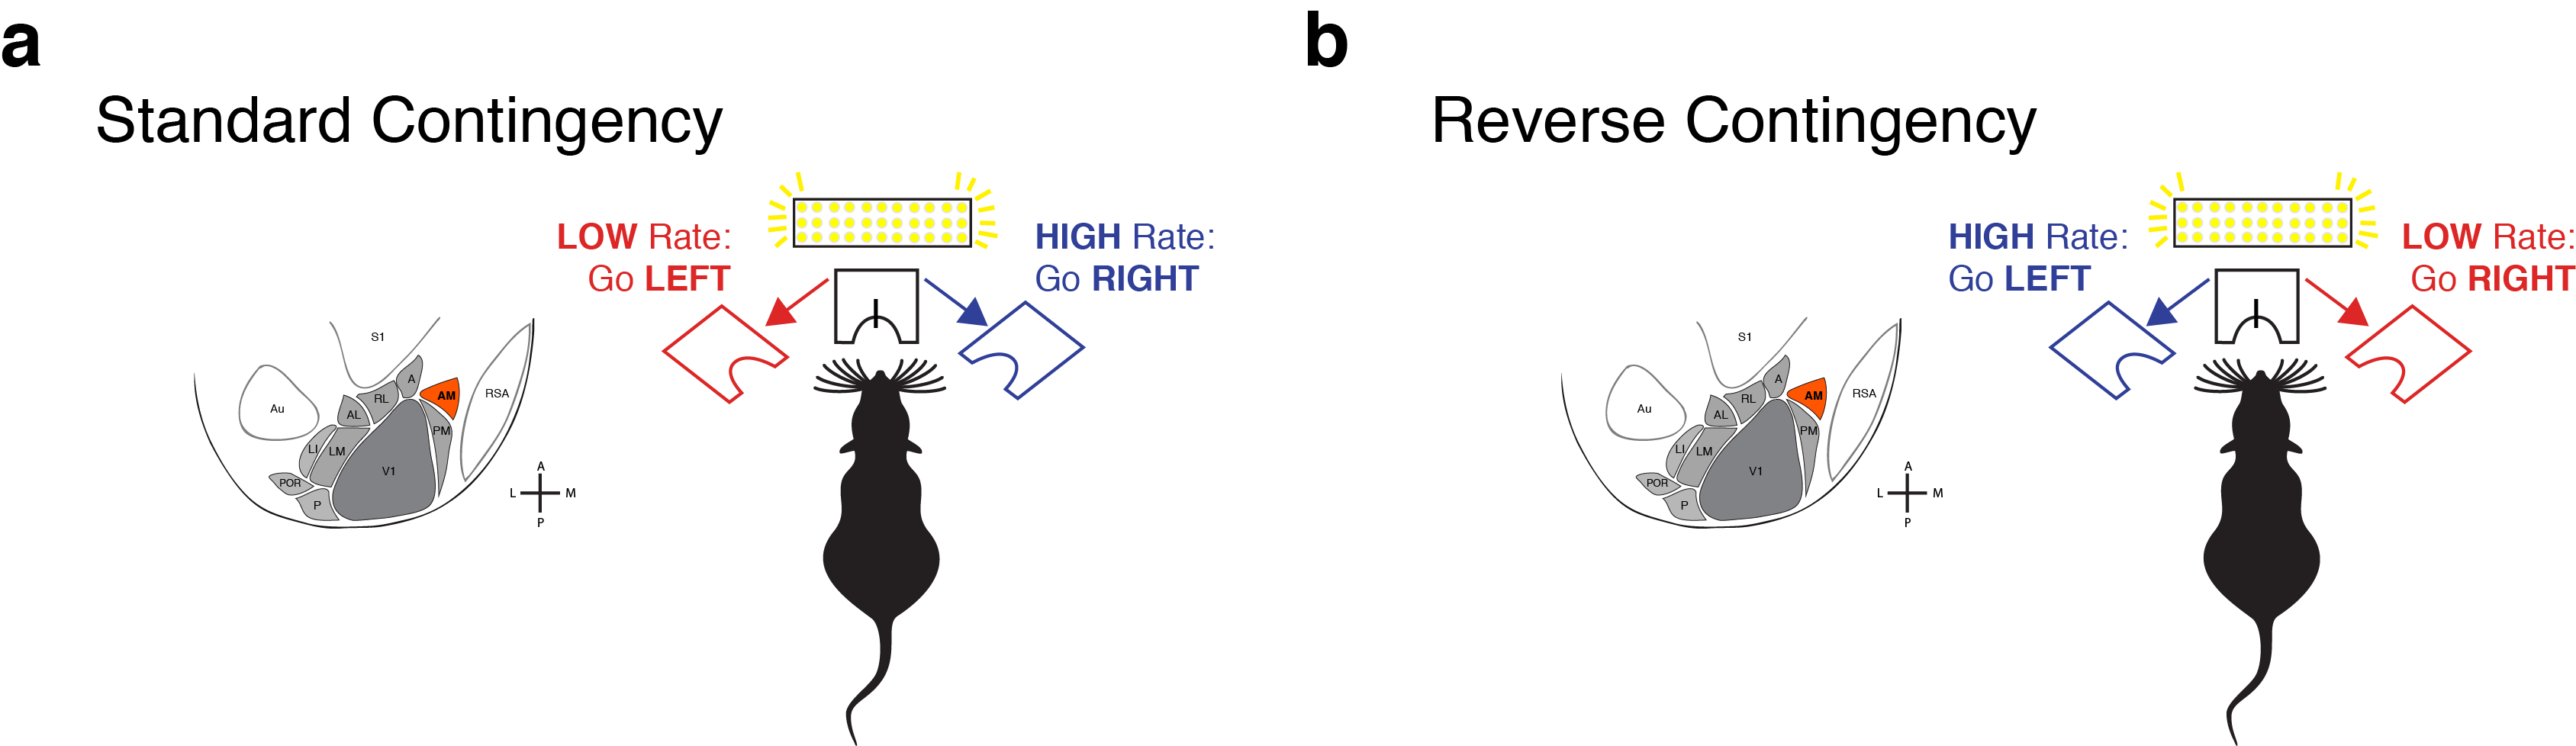
\includegraphics[width=\textwidth]{Figures/chapter4/jaws_AM_group2_schematic.png}
  \caption[Area AM Group 2 Cohort]{\textbf{Area AM Group 2 Cohort} (a) Group A trained on the standard contingency: High-Rate, go RIGHT (b) Group B trained on the reverse contingency: High-Rate, go LEFT. Jaws virus injected in and optical fiber implanted on the left hemisphere.}
   \label{fig:AMgroup2schem}
\end{figure}
%-----------------------------------------------------------------------------
\begin{figure}
  \centering
   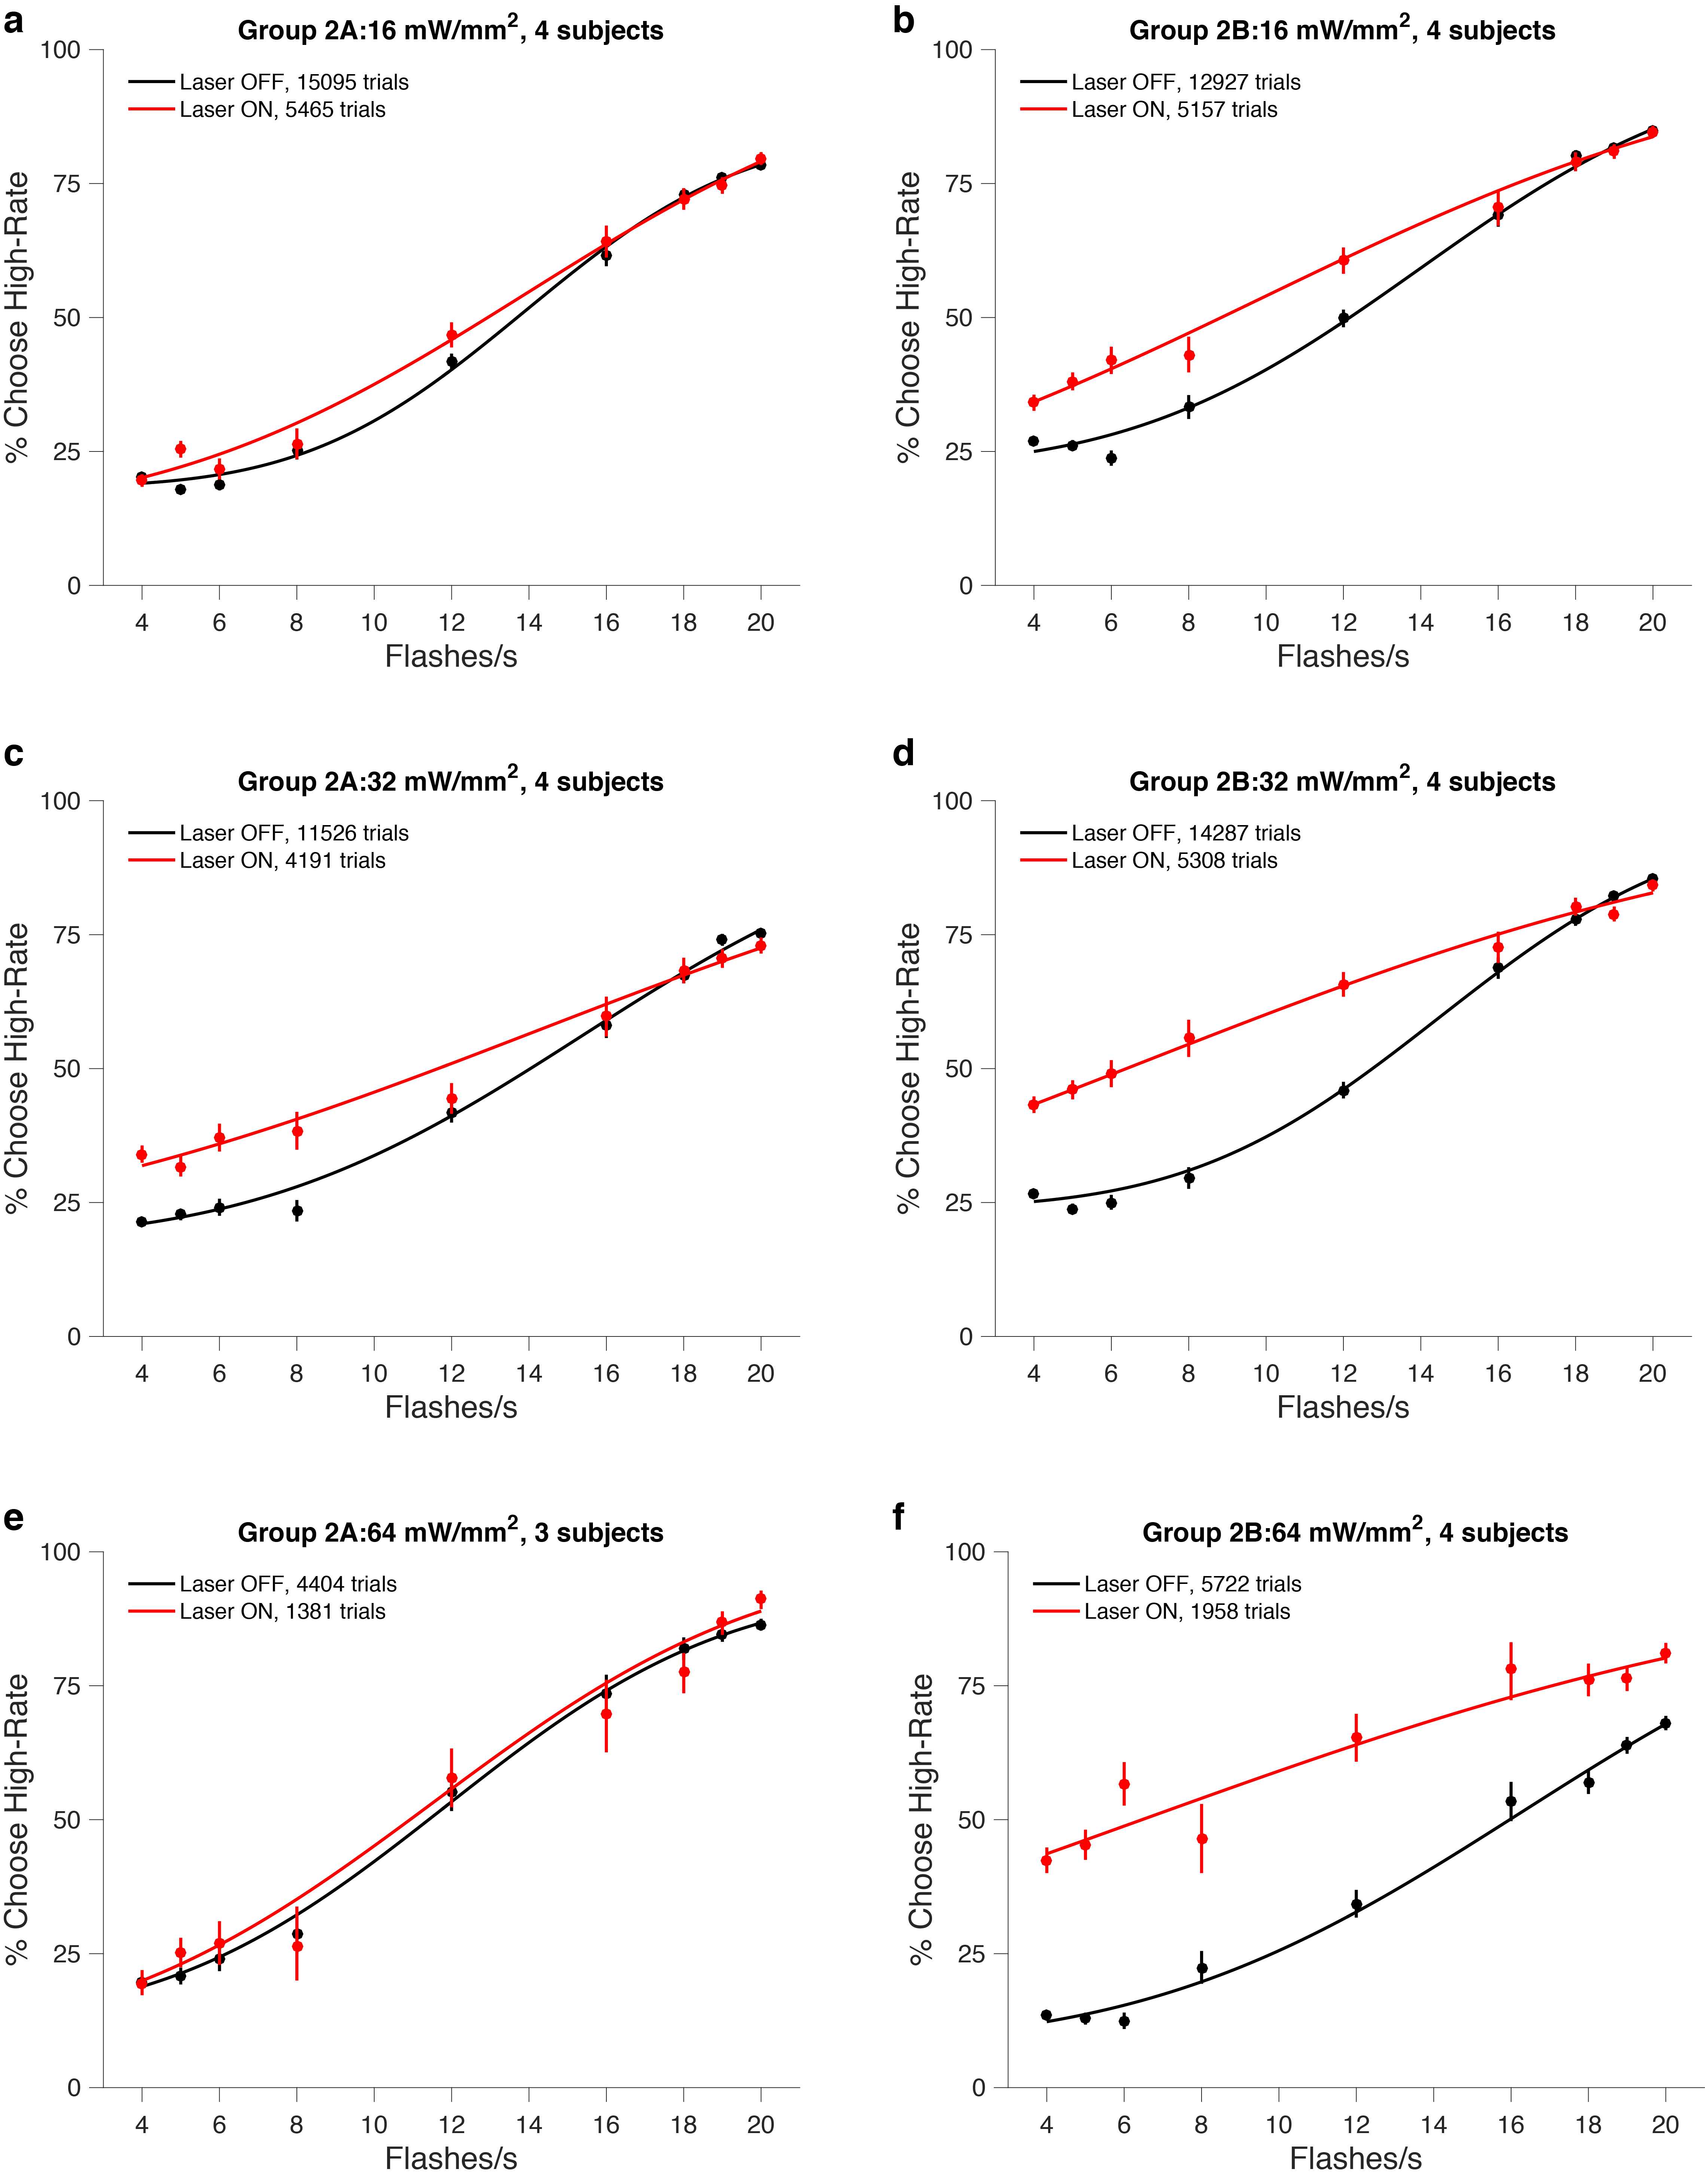
\includegraphics[width=\textwidth,height=0.9\textheight,keepaspectratio]{Figures/chapter4/jaws_AM_group2_summary_PMFs_irradiance.png}
  \caption[Area AM Group 2 Psychometric Data]{\textbf{Area AM Group 2 Psychometric Data} Pooled psychometric function at different irradiance levels for (a,c,e) Group 2A, standard contingency and (b,d,f) Group 2B, reverse contingency. Circles represent psychometric performance at each event rate and the solid line is the psychometric function fit with a cumulative Normal (Equation \ref{eq:normalpmf}). Errors bars represent Wilson binomial confidence intervals on the psychometric data.}
   \label{fig:AMgroup2summary}
\end{figure}
%-----------------------------------------------------------------------------
\begin{figure}
  \centering
   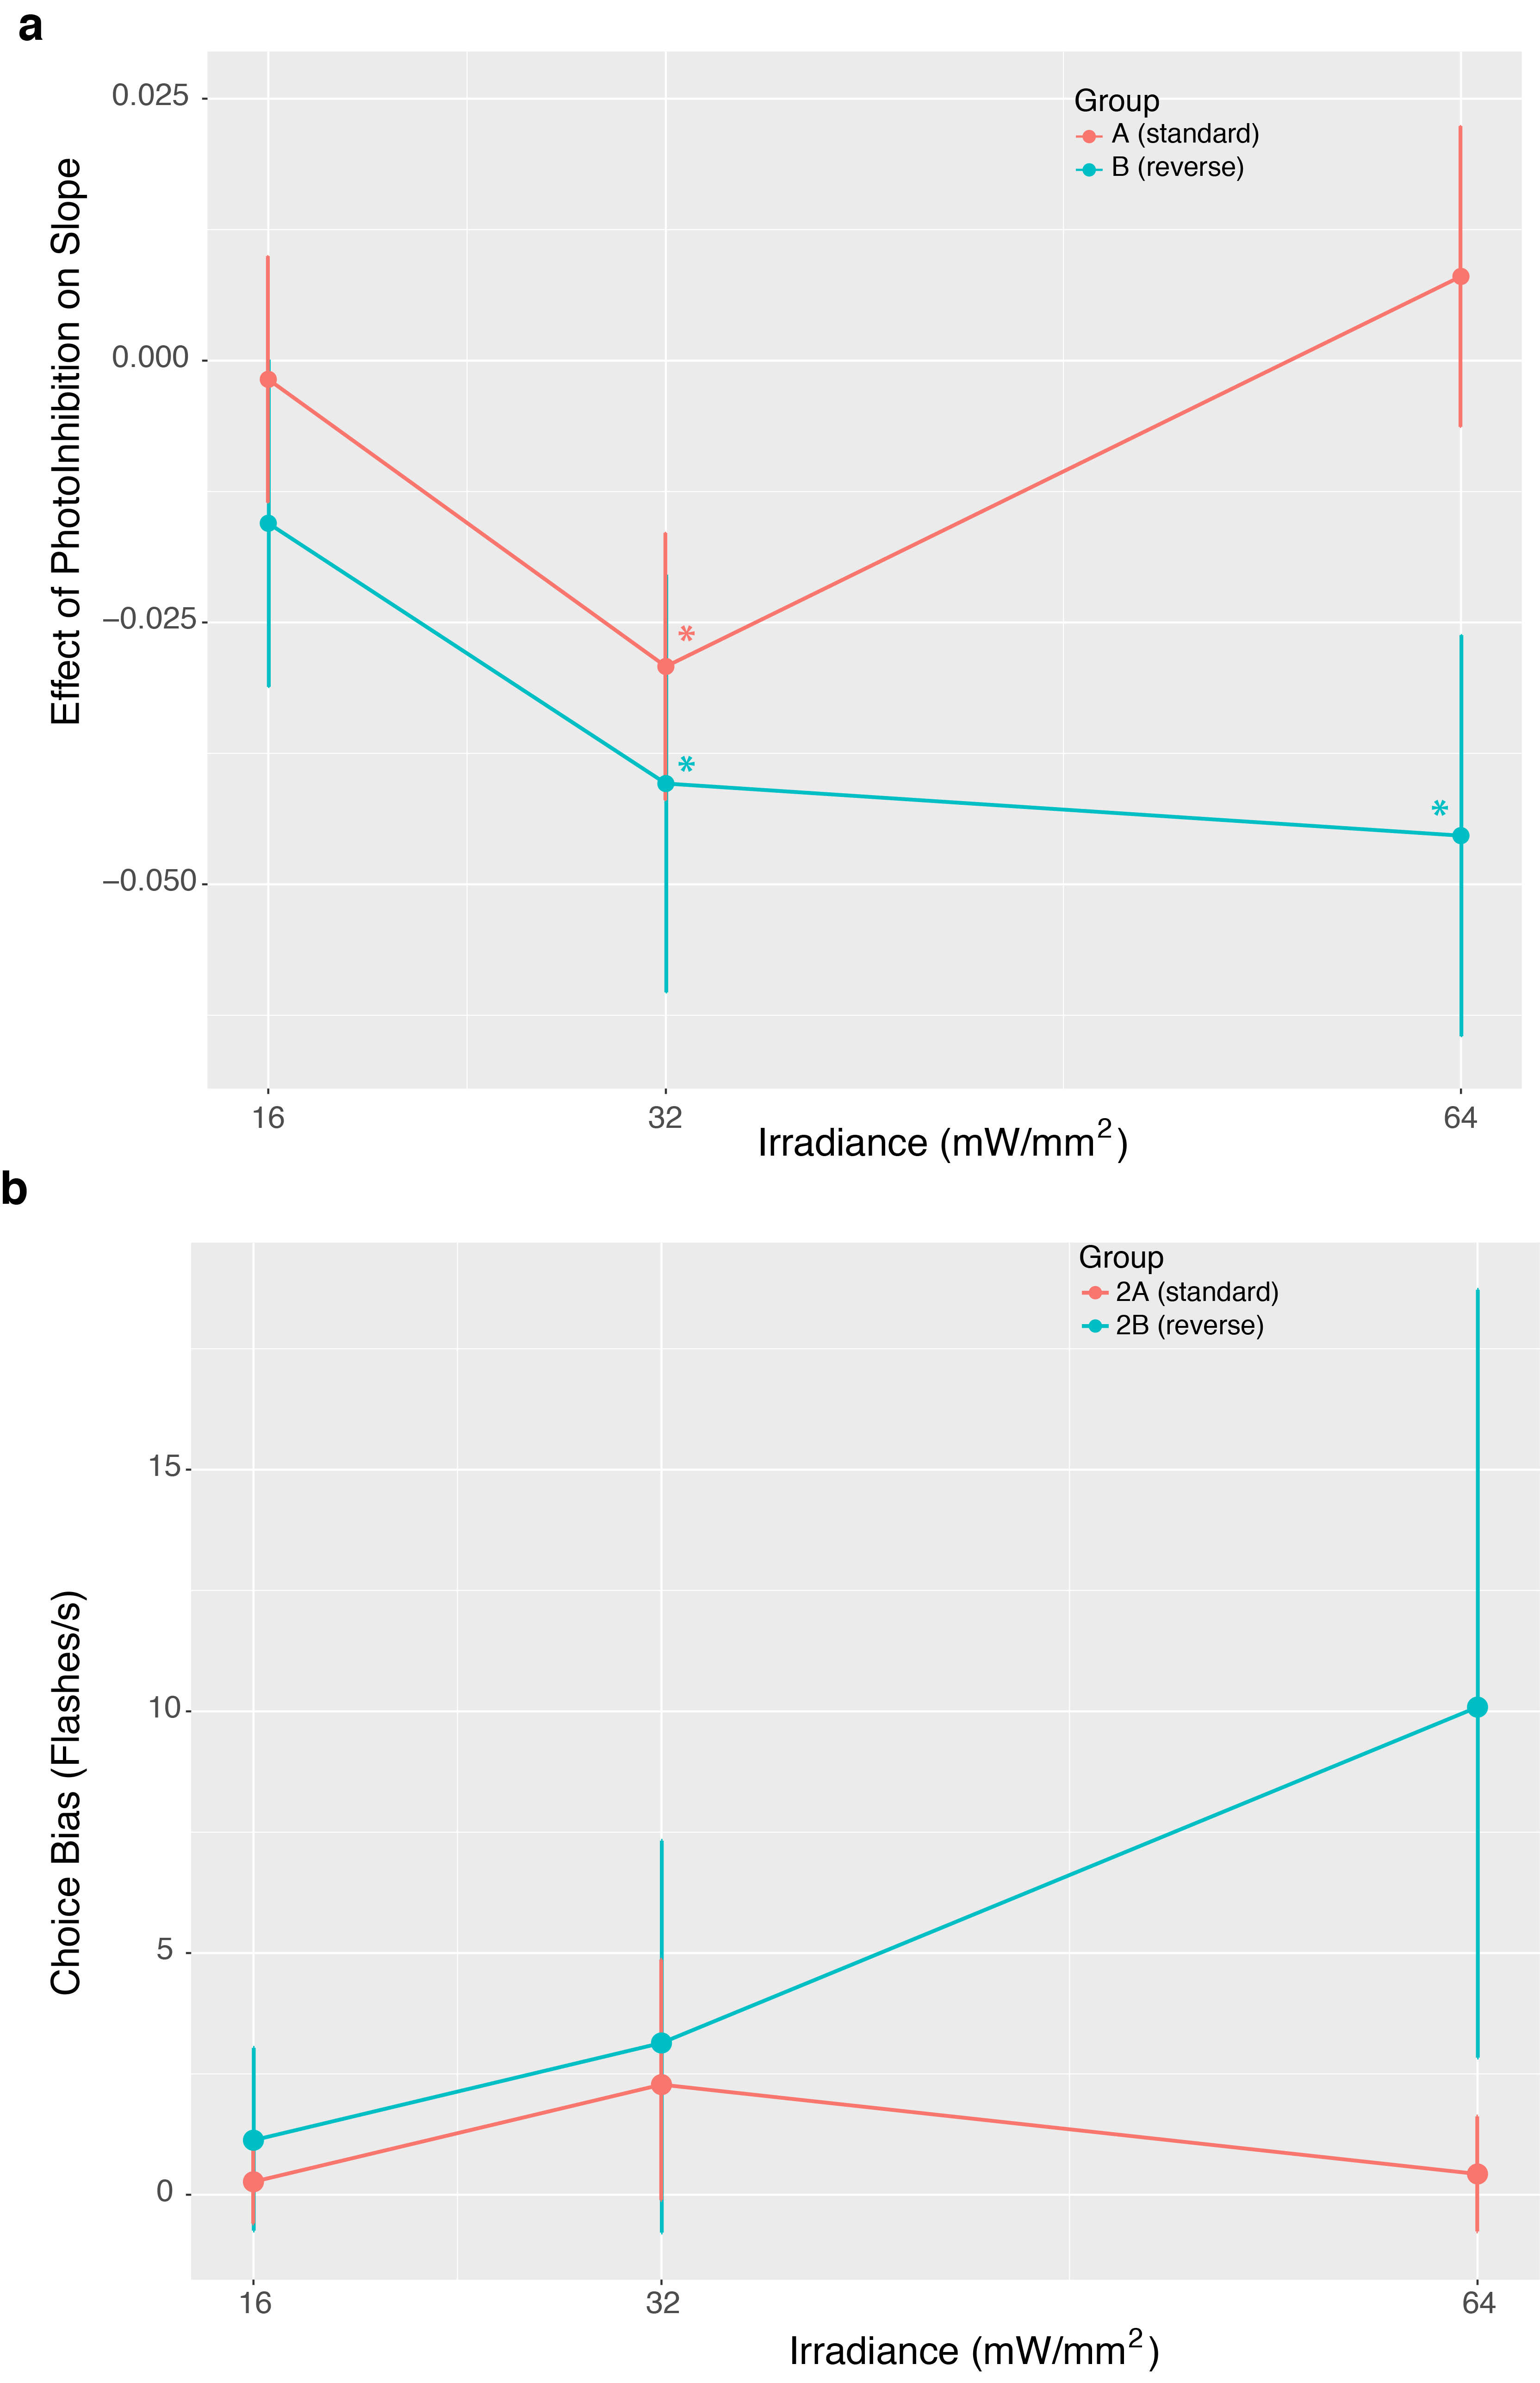
\includegraphics[width=\textwidth,height=0.9\textwidth,keepaspectratio]{Figures/chapter4/glmm_pmf_effects.png}
  \caption[Psychophysical Effects of Area AM Photoinhibition]{\textbf{Psychophysical Effects of Area AM Photoinhibition} Psychophysical parameters estimated from the GLMM model. (a) Effect of area AM photoinhibition on the slope of the psychometric function ($\beta_{evidence:opto}$) as a function of irradiance. Error bars represent 95\% confidence interval. Asterisks mark statistically significant (p<0.05) coefficients. (b) Choice bias as defined in Equation \ref{choicebias}. Choice bias error bars represent 95\% confidence intervals estimated by error propagation. }
   \label{fig:amGLMMparams}
\end{figure}

% %-----------------------------------------------------------------------------
% Figure \ref{fig:highRateBias} summarizes the high-rate bias for each animal. High-rate bias was measured as the difference between percent correct on high-rate choices and low-rate choices. 
% \begin{figure}
%   \centering
%    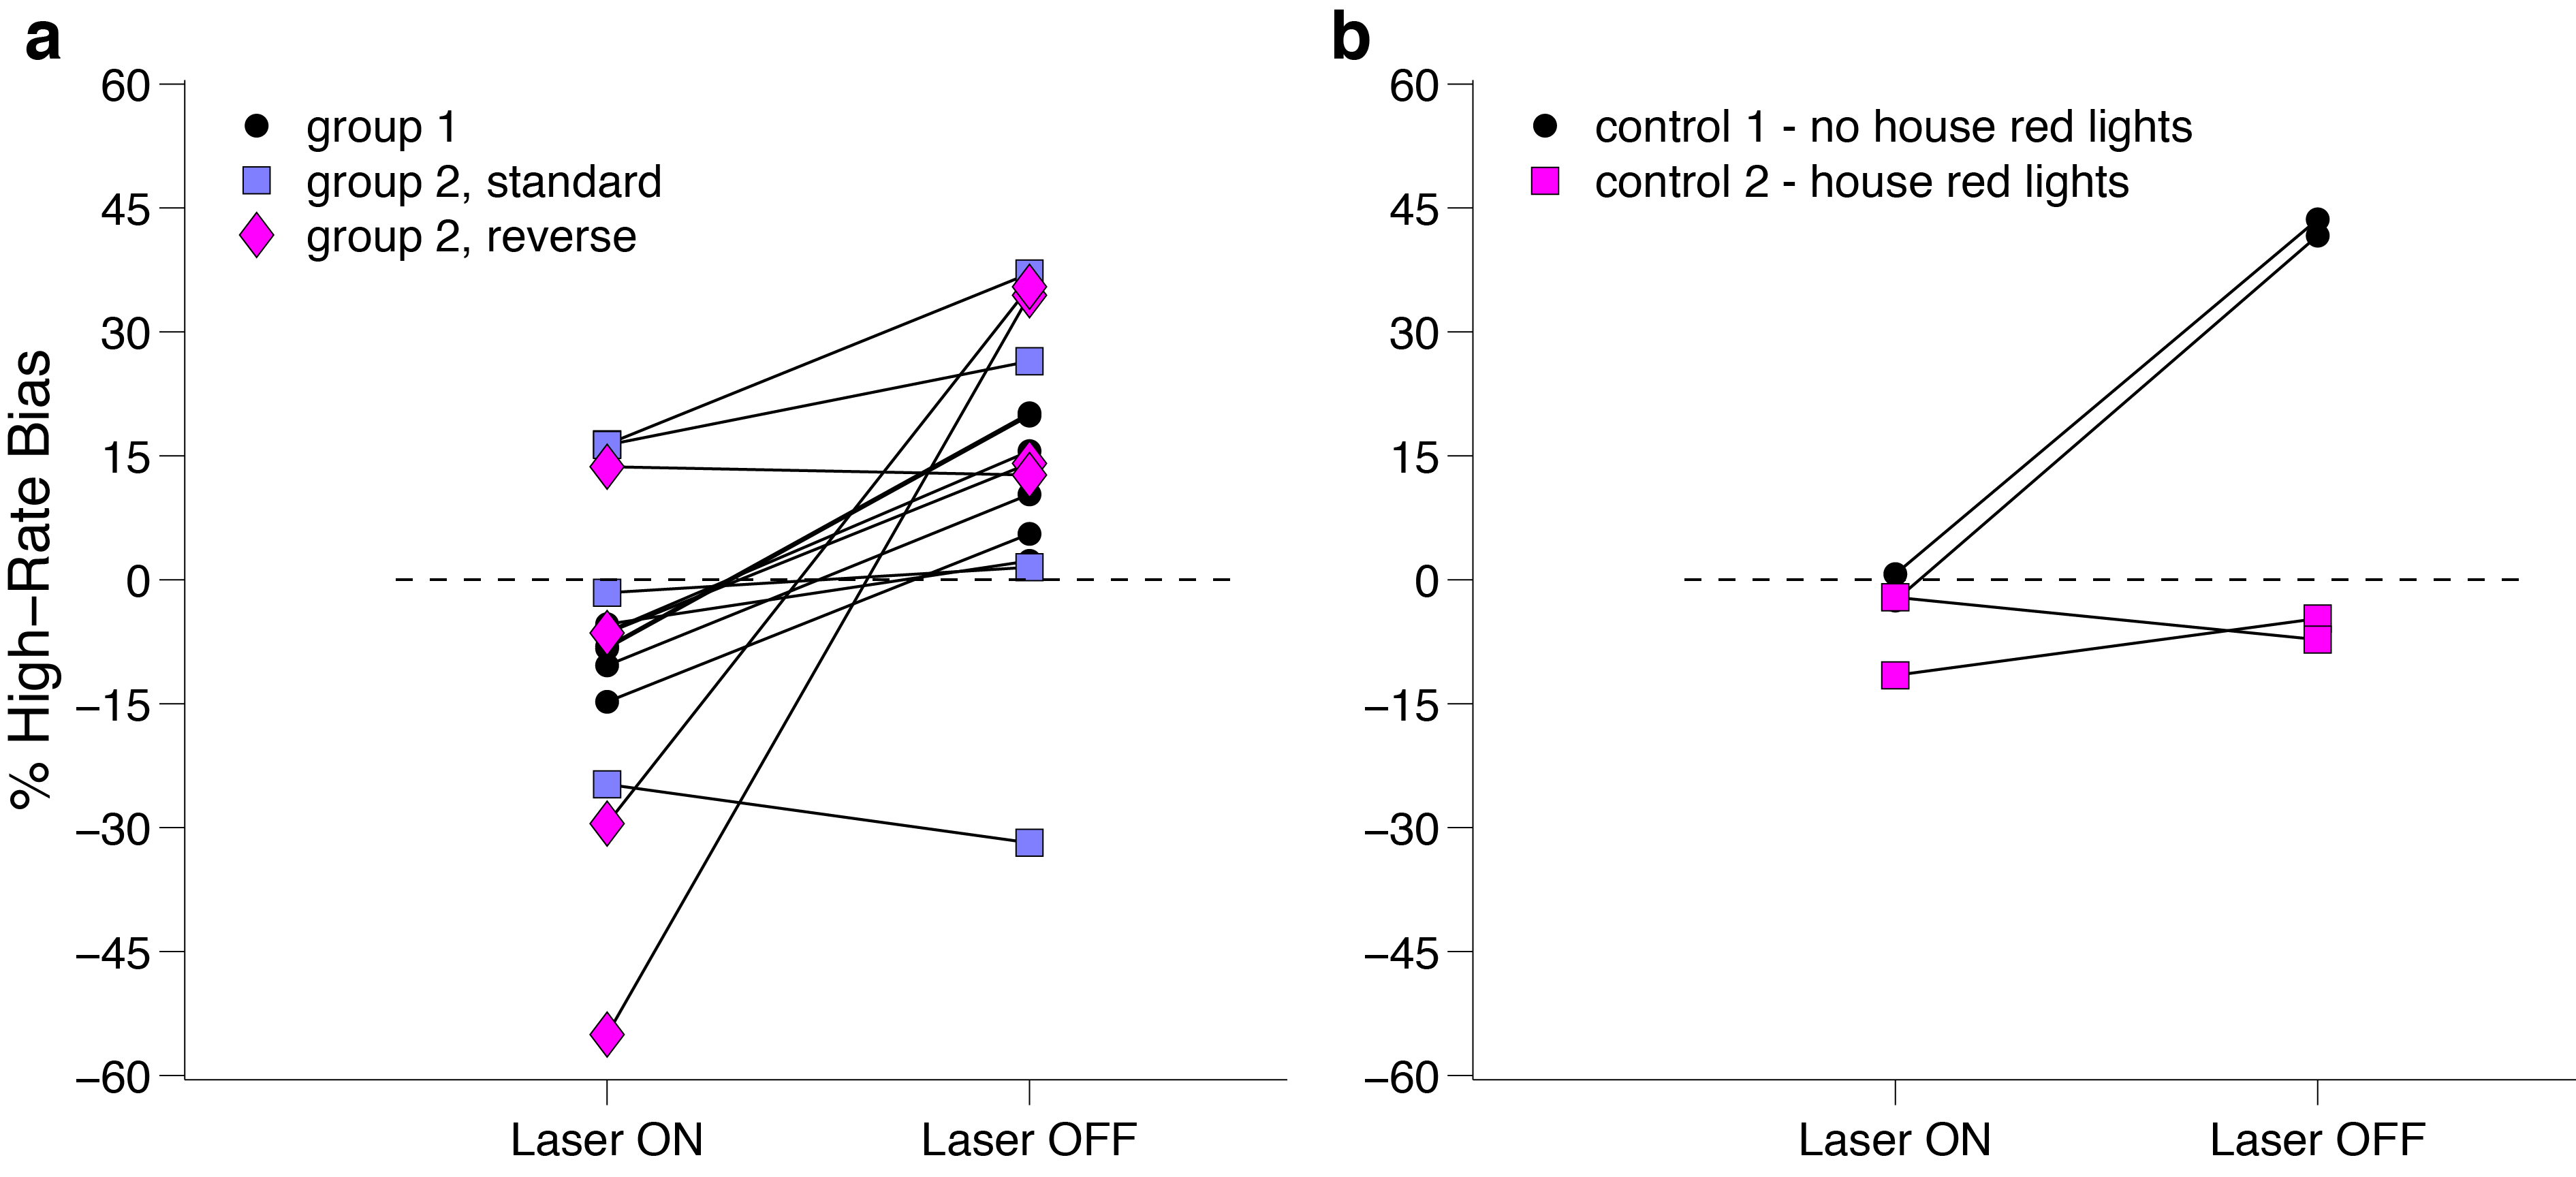
\includegraphics[scale=0.45]{Figures/chapter4/highRateBias.png}
%   \caption[]{\textbf{High-Rate Bias, all mice} }
%    \label{fig:highRateBias}
% \end{figure}
%-----------------------------------------------------------------------------
\section{Discussion}
In this chapter, I presented experiments aimed at silencing mouse secondary visual area AM during visual evidence accumulation. Photoinhibition affected both the sensitivity and choice bias in both groups. However, there were noticeable differences in the effect of photoinhibition. Group 2B mice, implanted on the left hemisphere and trained on the reverse contingency (HIGH-Rate, Go LEFT), were more affected by area AM inhibition in terms of stimulus sensitivity and choice bias (Figure \ref{fig:amGLMMparams}), compared to Group 2A mice trained on the standard contingency. Group 2B mice exhibited a greater tendency to make more high-rate choices during AM photoinhibition, in addition to an ipsilateral bias towards the fiber implanted hemifield. This effect is also consist with that observed in Group 1 mice, who were trained in the absence of the masking red light. \par 

A plausible explanation for the observed differences between the two groups is unilateral photoinhibition of area AM causes a bias towards the ipsilateral hemisphere. However, this effect is combined with the residual high-rate artifact caused by \emph{in vivo} red light stimulation (Figures \ref{fig:ctrlsummary} and \ref{fig:ctrlpmfs}). In Group 2B mice, the photoinhibition site (located on the left hemisphere) and high-rate (left hemifield) choice port are congruent, hence upon photoinhibition the effect area AM photoinhibition and the red light artifact sum together to produce the apparent high-rate bias. On the other hand, in Group 2A mice, the photoinhibition site (left hemisphere) and high-rate choice port (right hemifield) are incongruent; hence, the effect of area AM inhibition and the red light artifact would compete, and in some regimes cancel each other. Consistent with this hypothesis, at 64 mW/mm$^{2}$ photoinhibition Group 2A mice exhibit no change in choice bias or the sensitivity. However at 32 mW/mm$^{2}$ the choice bias tends toward positive, and may be a result of the residual red light artifact which is greater than the proposed ipsilateral bias effect caused by area AM inhibition. \par

The confound introduced by the red light source used for photoinhibition makes it difficult to disentangle the true nature of the effect of area AM photoinhibition. The artifact was greatly reduced (Figure \ref{fig:glmmcontrol}), although not eliminated, by training the mice with house red lights (Figure \ref{fig:ctrlpmfs}). The artifact is most likely caused by red light propagating from the stimulation site and directly activating the retina from within \parencite{Danskin2015} and producing an apparent increase in overall brightness, which is correlated with the high-rate flashes (Figure \ref{fig:brightnessSim}). \textcite{Danskin2015} measured retinal activation during \emph{in vivo} red light stimulation and found the largest activation ipsilateral to the implanted stimulation fiber. This would imply that mice would have an increased tendency to go towards the hemifield ipsilateral to the implanted fiber. Since the visual pulses stimuli is non-spatial it is unlikely that the mice are directly biased towards the implant site. Instead, the behavioral artifact of red light stimulation might arise if the mice were using perceived brightness over time as a strategy to solve the visual pulses task. The nature of the visual pulses stimulus is such that the average brightness (or amount of photons) over time is correlated with the number of flashes (Figure \ref{fig:brightnessSim}). The high-rate stimulus is the stimulus that is also the brightest or emits the most number of photons over time and conversely the low-rate stimulus emits the least number of photons over time. Hence, during \emph{in vivo} red light stimulation, the light escaping the eyes combines with the incoming light from the visual pulses stimuli and increases the perceived brightness (Figure \ref{fig:brightnessSim}b). This may cause the animal to make a high-rate choice. Brightness manipulation experiments on the visual pulses task (Chapter \ref{Chapter2}) suggests that the psychophysical performance of the mice is not entirely invariant to changes in the brightness of the flashes, and that mice may be using a combination of individual flash counting and perceived brightness over time to solve the task.\par 
%-----------------------------------------------------------------------------
\begin{figure}
  \centering
   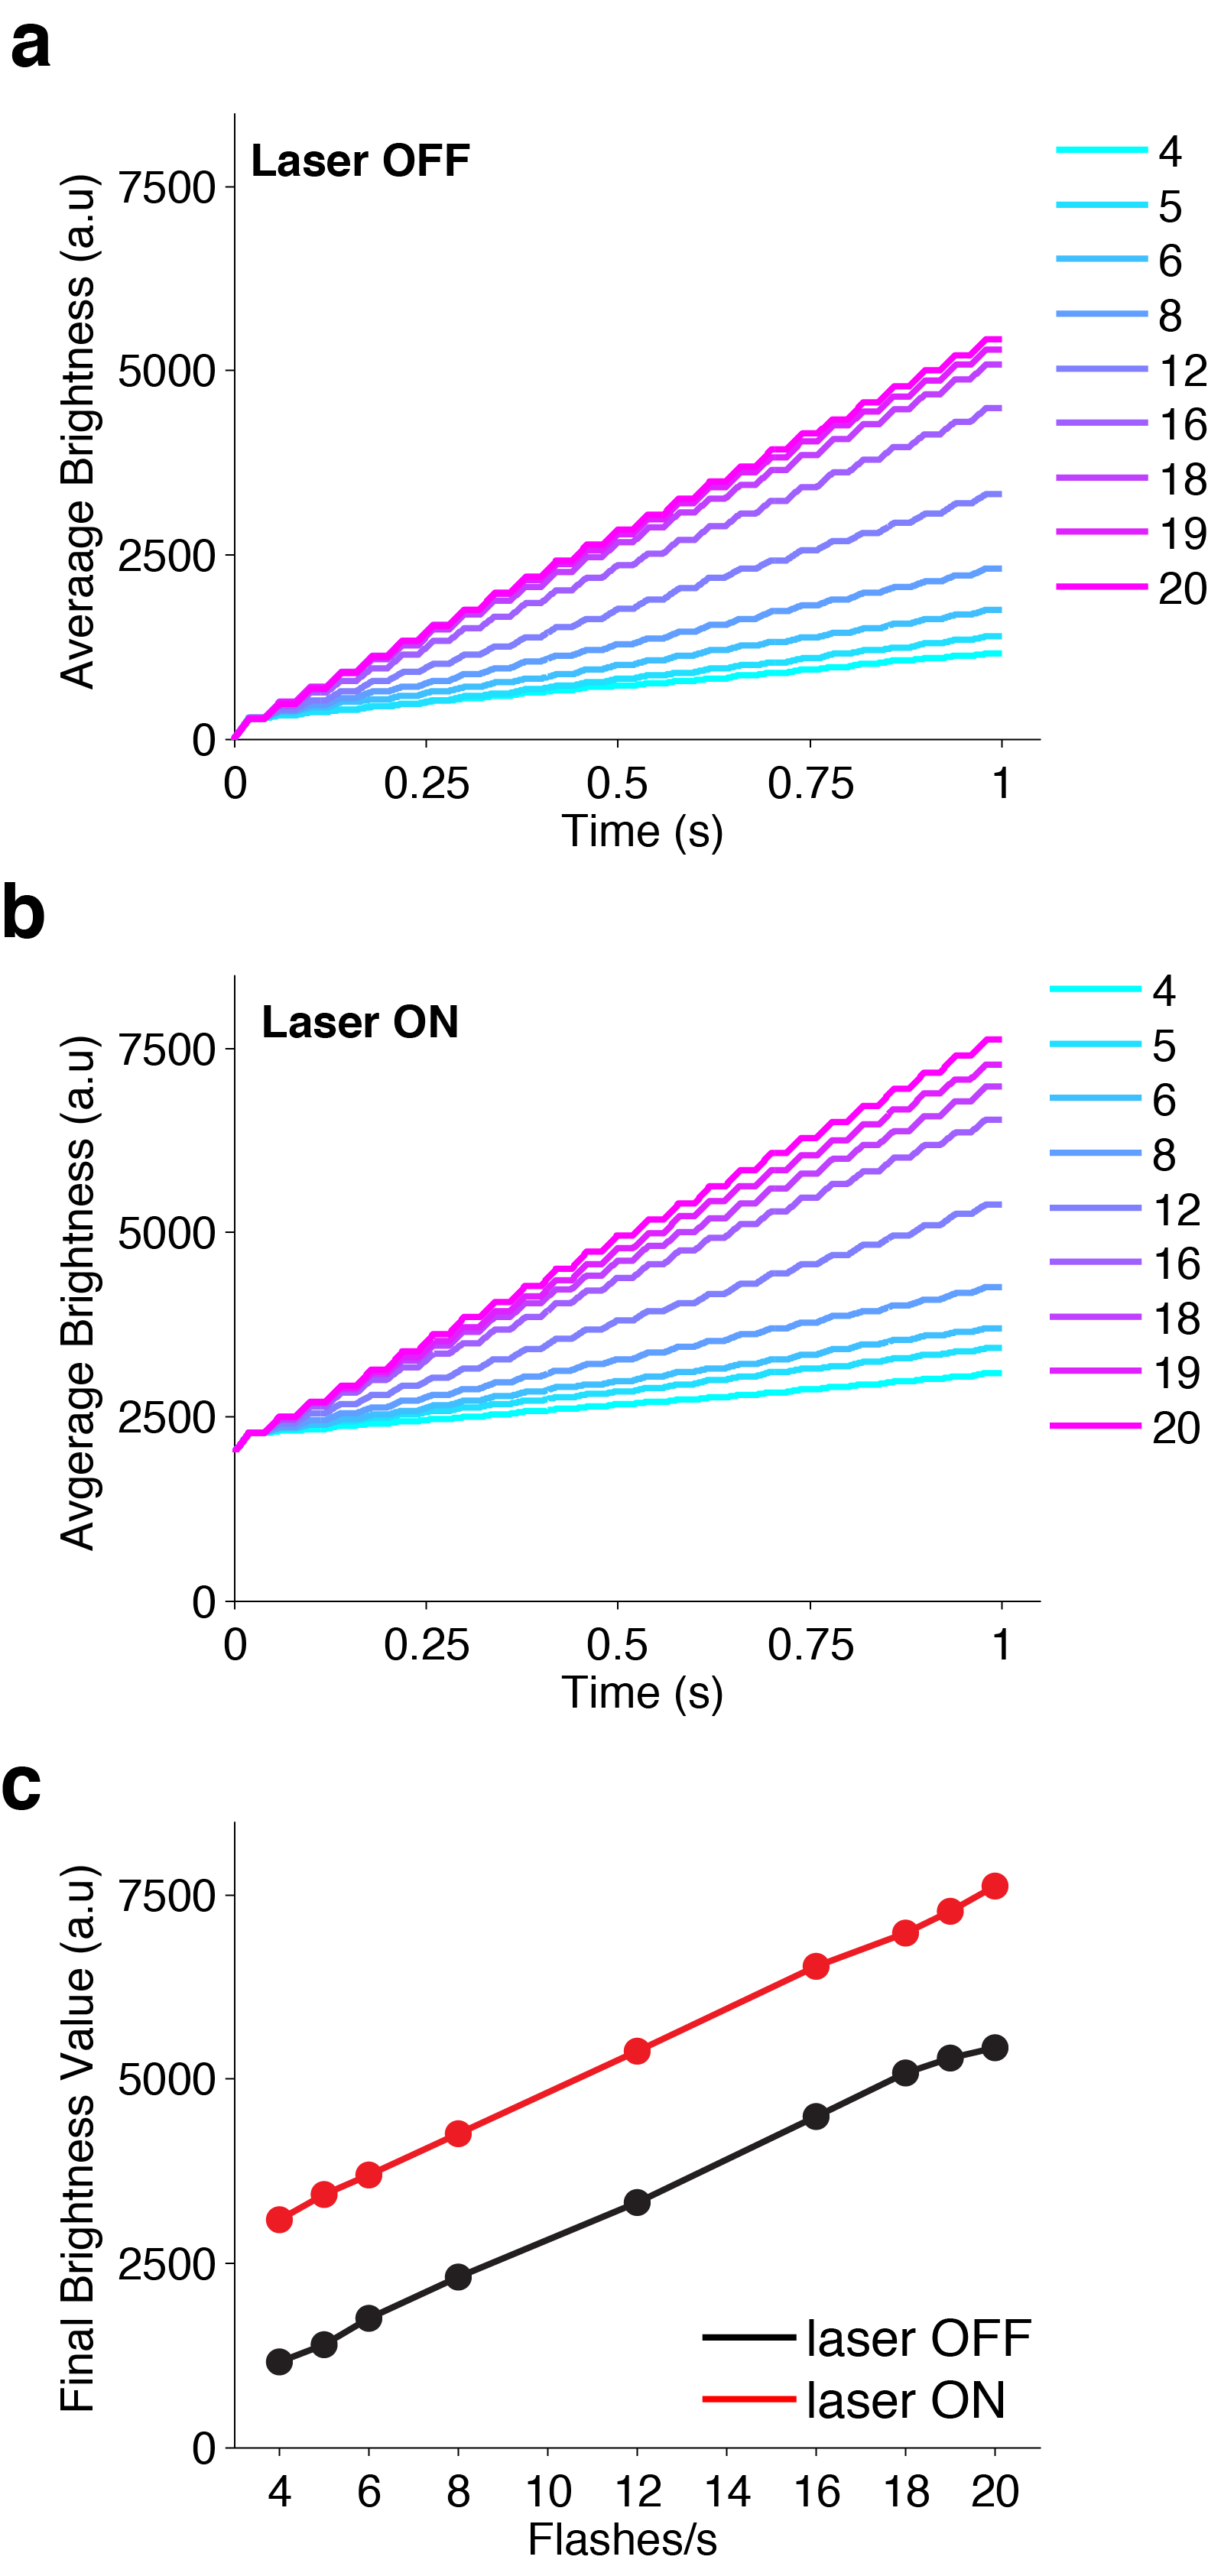
\includegraphics[width=\textwidth,height=0.9\textheight,keepaspectratio]{Figures/chapter4/brightnes_simulation_opto.png}
  \caption[Schematic of Simulated Average Apparent Brightness Over Time]{\textbf{Schematic of Simulated Average Apparent Brightness Over Time} (a) for laser off and (b) laser on condition.(c) The final value from Figure \ref{fig:brightnessSim} plotted against the number of flashes per second for laser OFF (black) and laser ON (red) conditions.}
   \label{fig:brightnessSim}
\end{figure}
%-----------------------------------------------------------------------------
%-----------------------------------------------------------------------------

\begin{table}
\centering
\resizebox{\textwidth}{!}{%
\begin{tabular}{@{}cccccccc@{}}
\toprule
\textbf{Group} & \textbf{\begin{tabular}[c]{@{}c@{}}Sample\\ Size\end{tabular}} & \textbf{\begin{tabular}[c]{@{}c@{}}Implant\\  Side\end{tabular}} & \textbf{\begin{tabular}[c]{@{}c@{}}High-Rate \\ Side\end{tabular}} & \textbf{\begin{tabular}[c]{@{}c@{}}Masking\\ Light\end{tabular}} & \textbf{\begin{tabular}[c]{@{}c@{}}Irradiance\\ (mW/mm\textasciicircum 2)\end{tabular}} & \textbf{\begin{tabular}[c]{@{}c@{}}Interaction\\ b\_evid:opto\end{tabular}} & \textbf{\begin{tabular}[c]{@{}c@{}}Choice Bias\\ (Flashes/s)\end{tabular}} \\ \midrule
\textbf{1} & 6 & R & R & No & 32 & \begin{tabular}[c]{@{}c@{}}-0.021*\\ {[}-0.034   -0.0085{]}\end{tabular} & \begin{tabular}[c]{@{}c@{}}3.47\\ {[}2.46   4.54{]}\end{tabular} \\
\textbf{Control} & 2 & R & R & No & 32 & \begin{tabular}[c]{@{}c@{}}-0.038*\\ {[}-0.056  -0.020{]}\end{tabular} & \begin{tabular}[c]{@{}c@{}}9.72\\ {[}6.3   13.60{]}\end{tabular} \\
\textbf{} &  &  &  & Yes & 64 & \begin{tabular}[c]{@{}c@{}}-0.026*\\ {[}-0.044 -0.0085{]}\end{tabular} & \begin{tabular}[c]{@{}c@{}}2.244\\ {[}0.49   4.37{]}\end{tabular} \\
\textbf{2A} & 4 & L & R & Yes & 16 & \begin{tabular}[c]{@{}c@{}}-0.0018\\ {[}-0.014   9.97e-03{]}\end{tabular} & \begin{tabular}[c]{@{}c@{}}0.27\\ {[}-0.60  1.14{]}\end{tabular} \\
\textbf{} &  &  &  & Yes & 32 & \begin{tabular}[c]{@{}c@{}}-0.029*\\ {[}-0.042   -1.64e-02{]}\end{tabular} & \begin{tabular}[c]{@{}c@{}}2.28\\ {[}-0.092  4.84{]}\end{tabular} \\
\textbf{} &  &  &  & Yes & 64 & \begin{tabular}[c]{@{}c@{}}0.008\\ {[}-0.0063   2.24e02{]}\end{tabular} & \begin{tabular}[c]{@{}c@{}}0.43\\ {[}-0.75  1.62{]}\end{tabular} \\
\textbf{2B} & 4 & L & L & Yes & 16 & \begin{tabular}[c]{@{}c@{}}-0.016\\ {[}-0.031   8.83e-05{]}\end{tabular} & \begin{tabular}[c]{@{}c@{}}1.13\\ {[}-0.76  3.045{]}\end{tabular} \\
\textbf{} &  &  &  & Yes & 32 & \begin{tabular}[c]{@{}c@{}}-0.040*\\ {[}-0.06   -2.2e-02{]}\end{tabular} & \begin{tabular}[c]{@{}c@{}}3.14\\ {[}-0.75  7.28{]}\end{tabular} \\
\textbf{} &  &  &  & Yes & 64 & \begin{tabular}[c]{@{}c@{}}-0.045*\\ {[}-0.064   -2.62e-02{]}\end{tabular} & \begin{tabular}[c]{@{}c@{}}10.09\\ {[}2.84  18.72{]}\end{tabular} \\ \bottomrule
\end{tabular}%
}
\caption[GLMM Analysis Summary Table]{\textbf{GLMM Analysis Summary Table}. * statistically significant coefficients (p < 0.05) }
\label{table:glmm}
\end{table}
%-----------------------------------------------------------------------------%-----------------------------------------------------------------------------

The proposed ipsilateral bias caused by AM photoinhibition is consistent with spatial hemineglect observed in visual parietal lesions. Spatial hemineglect, also referred to as contralateral neglect, is a phenomenon that occurs when subjects ignore the contralateral hemifield as a result of lesion to the parietal cortex. Although hemineglect has been observed in humans \parencite{Stone1991,Kerkho2001} and rats \parencite{Crowne1986,Reep2009}, it is not clear whether neglect has been observed in mice. The presence of hemispatial neglect would suggest that the mice are neglecting the tendency to go towards the affected (contralateral) visual hemifield. Therefore, in the presence of a red light artifact, mice trained on opposite behavioral contingencies should yield the same effect, i.e. a bias ipsilateral to the stimulation hemisphere. \par 

Another related, and plausible, interpretation for the ipsilateral bias due to suppression of AM activity is that neurons in AM likely represents the "intent" to make contralateral choices. Intention, in the neuroscience literature, is defined as an early plan for movement, which specifies the goal and type of movement \parencite{Andersen2002}. Under the intention scenario, the two hemispheres of AM would represent competing movement intentions, such that inactivation of one hemisphere leads to movement in the opposing direction. 
%This framework makes an interesting prediction for bilateral inactivation of AM. In this scenario, the psychometric function would appear shallower (Figure \ref{fig:predictions}b) reflecting a loss in sensitivity as contralateral movement intentions on both hemispheres are impaired. \par 

To test the proposed spatial hemineglect (or impaired intent) caused by area AM inhibition, one could train mice on a visual pulses task with two additional interspersed conditions: instructed and free choice \parencite{Erlich2015,Katz2016}. On the instructed trials, the animals are cued to a the reward port by a brief LED flash at the reward port, and in the free choice trials, both LEDs are turned on and the animal can freely choose either reward port to receive the reward. If visual area AM plays a role in spatial neglect (or contralateral movement intent), inactivation should only affect free choice trials and not the instructed trials. Because the animal chooses where to go on the free choice trials, if area AM plays a role in the intent to make contralateral movements, unilateral inactivation of area AM would bias the subject towards the hemifield ipsilateral to the stimulation site.\par 

For this study, Jaws was an attractive inhibitory opsin to use primarily because it outperformed other available inhibitory opsins such as ArchT and Halo in terms of inhibition \parencite{Chuong2014}. Despite the powerful inhibition afforded by Jaws, future studies would benefit from avoiding red light sensitive opsins altogether for experiments in mice performing visually-guided behaviors. Further efforts are needed to carefully characterize available optogenetic inhibitory tools that provide potent inhibition and do not interfere with the behavior. This requirement is dependent on the several factors such as the nature of the task, stimulus, and brain area(s) of interest. Nevertheless, several alternative optogenetic strategies are available, including blue light sensitive anion conducting channelrhodopsin (SwiChR or iC1C2) \parencite{Berndt2014,Berndt2016} or excitation of inhibitory neurons \parencite{Madisen2012,Glickfeld2013b,Poort2015,Burgess2016}. The latter approach presents a technical challenge for working with GCaMP6 transgenic mice, which are typically bred to express GCaMP6 in excitatory neurons \parencite{Madisen2015}. One could produce transgenic mice that express GCaMP6 in the inhibitory neurons (PV+ or Gad2+); however, it is not obvious whether mouse lines expressing GCaMP6 in inhibitory neurons could replicate the retinotopic widefield maps obtained with the existing GCaMP6 mouse lines. A solution that is compatible with the existing GCaMP6 transgenic line is a recent viral strategy that specifically targets inhibitory neurons \parencite{Dimidschstein2016}, by using a gene enhancer element, \emph{mDLx}. The viral strategy can be combined with conventional neural effectors such as channelrhodopsin to activate inhibitory neurons and silence the region(s) of interest.\par 

In summary, the results in this chapter provide promising evidence that support a role for visual area AM in visually-guided behavior involving the accumulation of evidence. The proposed role for AM, in this task, is that normal activity in AM drives contralateral choices, such that photoinhibition leads to an ipsilateral bias. This is consistent with AM's anatomical projections to motor areas, which strikingly resemble those observed in sensorimotor areas such as primate PPC. Hence, AM likely sits on the highway of transforming visual sensory inputs into motor actions. Further efforts are required to firmly establish these findings and its generalization to other visually-guided tasks in the mouse. 



 
\chapter{Decoding Natural Scene Images from Mouse Visual Cortex}
\label{Chapter5} 

In the previous chapters, mice were probed with an abstract, temporally rich, stimulus presented as a stochastic sequence of visual visuals. In real-world environments, stimuli are enriched not only in temporal content, but spatial content. In this chapter, I take a different approach to investigate how categorical information is distributed in extrastriate areas using neurophysiology data and for a different kind of stimuli - natural scenes. Mice have multiple visual areas, as mentioned in Chapter \ref{Chapter1}, (Figure \ref{fig:vis_areas} and \ref{fig:retinomap}). These visual areas possess distinct brain-wide projection patterns \parencite{Wang2012} and also distinct spatiotemporal response properties to grating stimuli  \parencite{Andermann2011,Marshel2011,Roth2012,Glickfeld2013a,Tohmi2014,Juavinett2015}. However, little is known as to whether mouse secondary visual areas also specialize in processing natural scene images. The goal of this chapter is to test whether the identity or category of natural scene images can be decoded from the neural population activity of distinct higher visual areas in the mouse.\par 

The brain, ultimately, uses information in complex scenes to recognize salient stimuli, discriminate amongst objects in a scene, and make decisions. Hierarchical visual processing is a hallmark of object recognition observed in the primate ventral stream pathway \parencite{DiCarlo2012}. To illustrate with an example, imagine you are faced with a task to discern between a car and a horse crossing the street. The information needed to make the categorization is already available at the level of the retina, however the information lives in a tangled and conflated representation. As the information progresses through various stages of visual processing along the ventral steam, the representations becomes more untangled, i.e. more linearly separable. Ultimately the distinction between the horse and the car are easily distinguishable and linearly separable in neural activity space. At the highest stage of visual processing, a linear boundary can be drawn between the neuronal population representation between the horse and the car. Linear readout (i.e. linear combinations) of neurons is an assumption for how downstream (postsynaptic) brain areas might theoretically integrate information represented in the neural responses of upstream (presynaptic) brain areas to ultimately generate an action.  

Population decoding analysis has been a fruitful tool for studying this type of high-level visual processing and revealing information represented within a neural population \parencite{Hung2005,Rust2010a,Pagan2013}. Population decoders (or classifiers) address questions such as, given neural population activity in a brain area, can information be read out about external variables in the world (eg. stimulus, choice)? In this chapter, I ask the following questions: how linearly separable are the neural responses to natural scenes? How does linear separability change across multiple visual areas and across cortical layers within an area? In other words, can a linear decoder read out the natural scene identity (or category) given the neural activity patterns in a given visual brain area or cortical layer? Since natural scenes are collection of objects, I drew inspiration from object recognition processing in primate ventral stream in considering how to address the proposed questions.  

To do this, I compared how natural scenes are processed in multiple mouse visual areas and cortical layers. More precisely I tested whether the neural population activity in response to distinct natural scenes was linearly separable. To this end, I trained a classifier to decoded the identity (or category) of natural scene images presented to mice, and compared the decoder accuracy across multiple visual areas and layers. The hypothesis is that activity in higher visual areas in response to natural scenes are linearly separable, consistent with an 'untangled' neural representation along the visual processing hierarchy. 

%-----------------------------------------------------------------------------
\begin{figure}
  \centering
   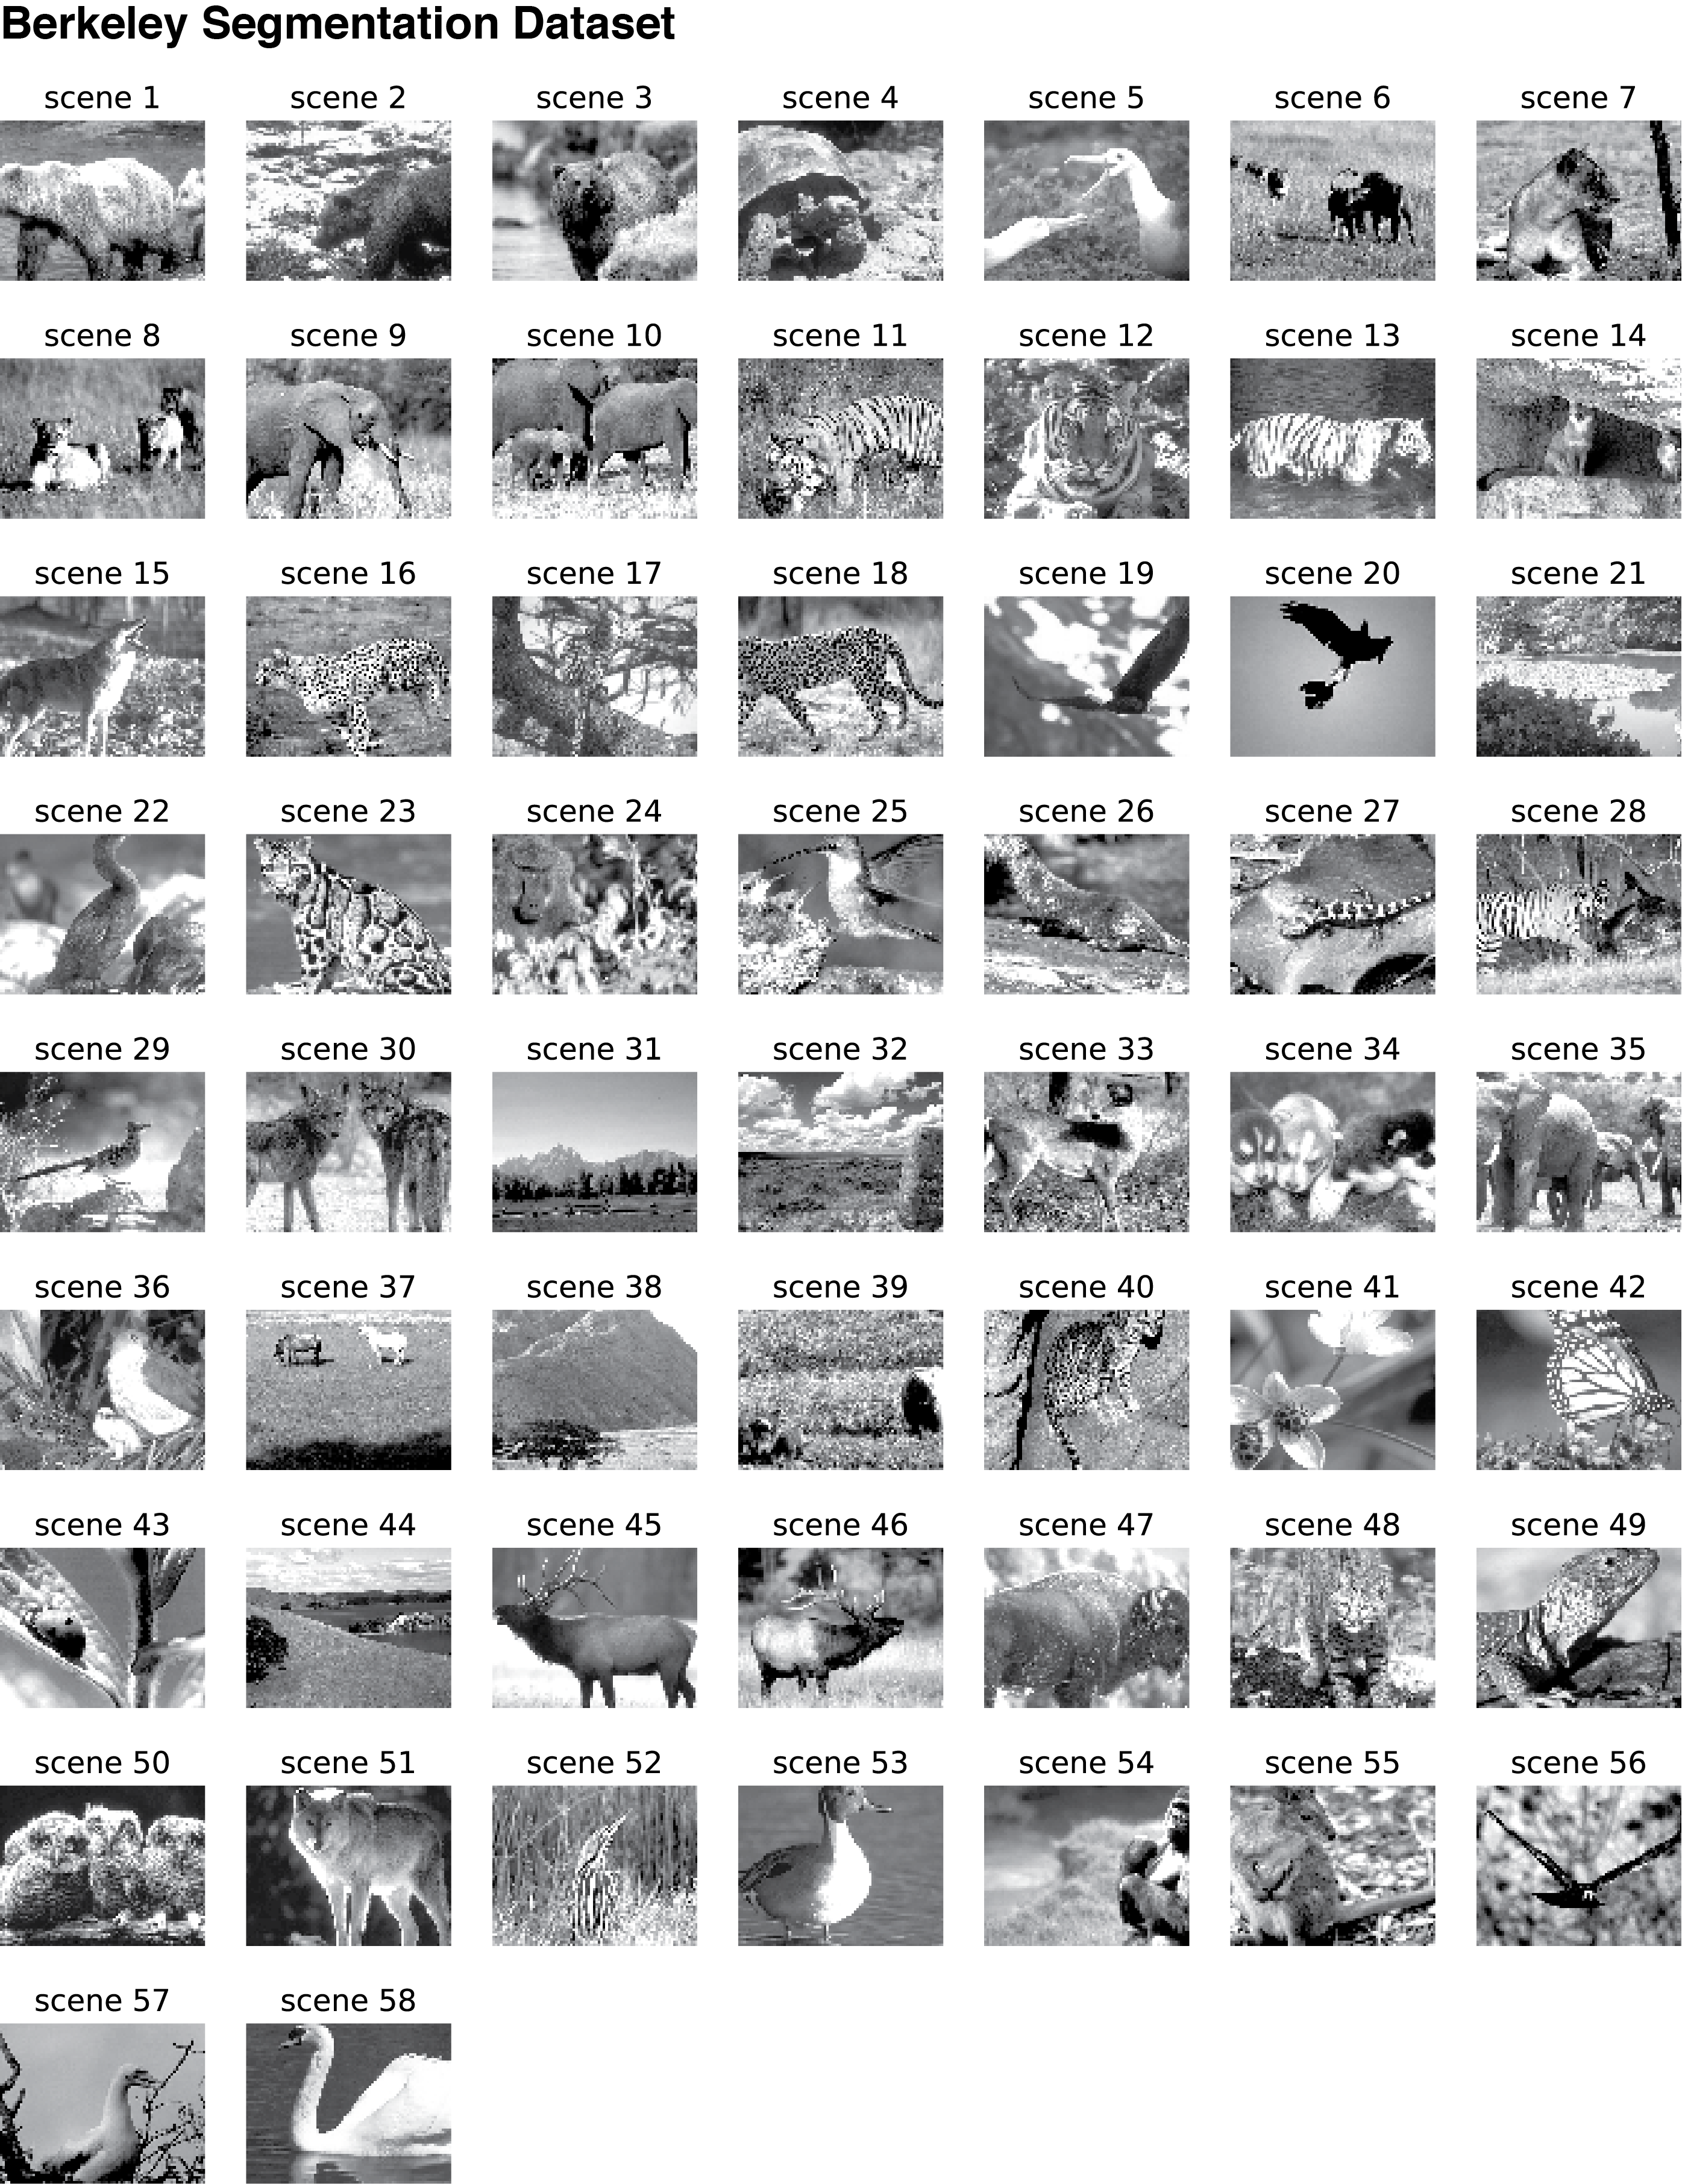
\includegraphics[width=\textwidth,height=0.9\textheight,keepaspectratio]{Figures/chapter5/images_dataset1.png}
  \caption[Thumbnail of Natural Images Stimulus Set - Part 1]{\textbf{Thumbnail of Natural Images Stimulus Set - Part 1} }
   \label{fig:images1}
\end{figure}
%-----------------------------------------------------------------------------
\begin{figure}
  \centering
   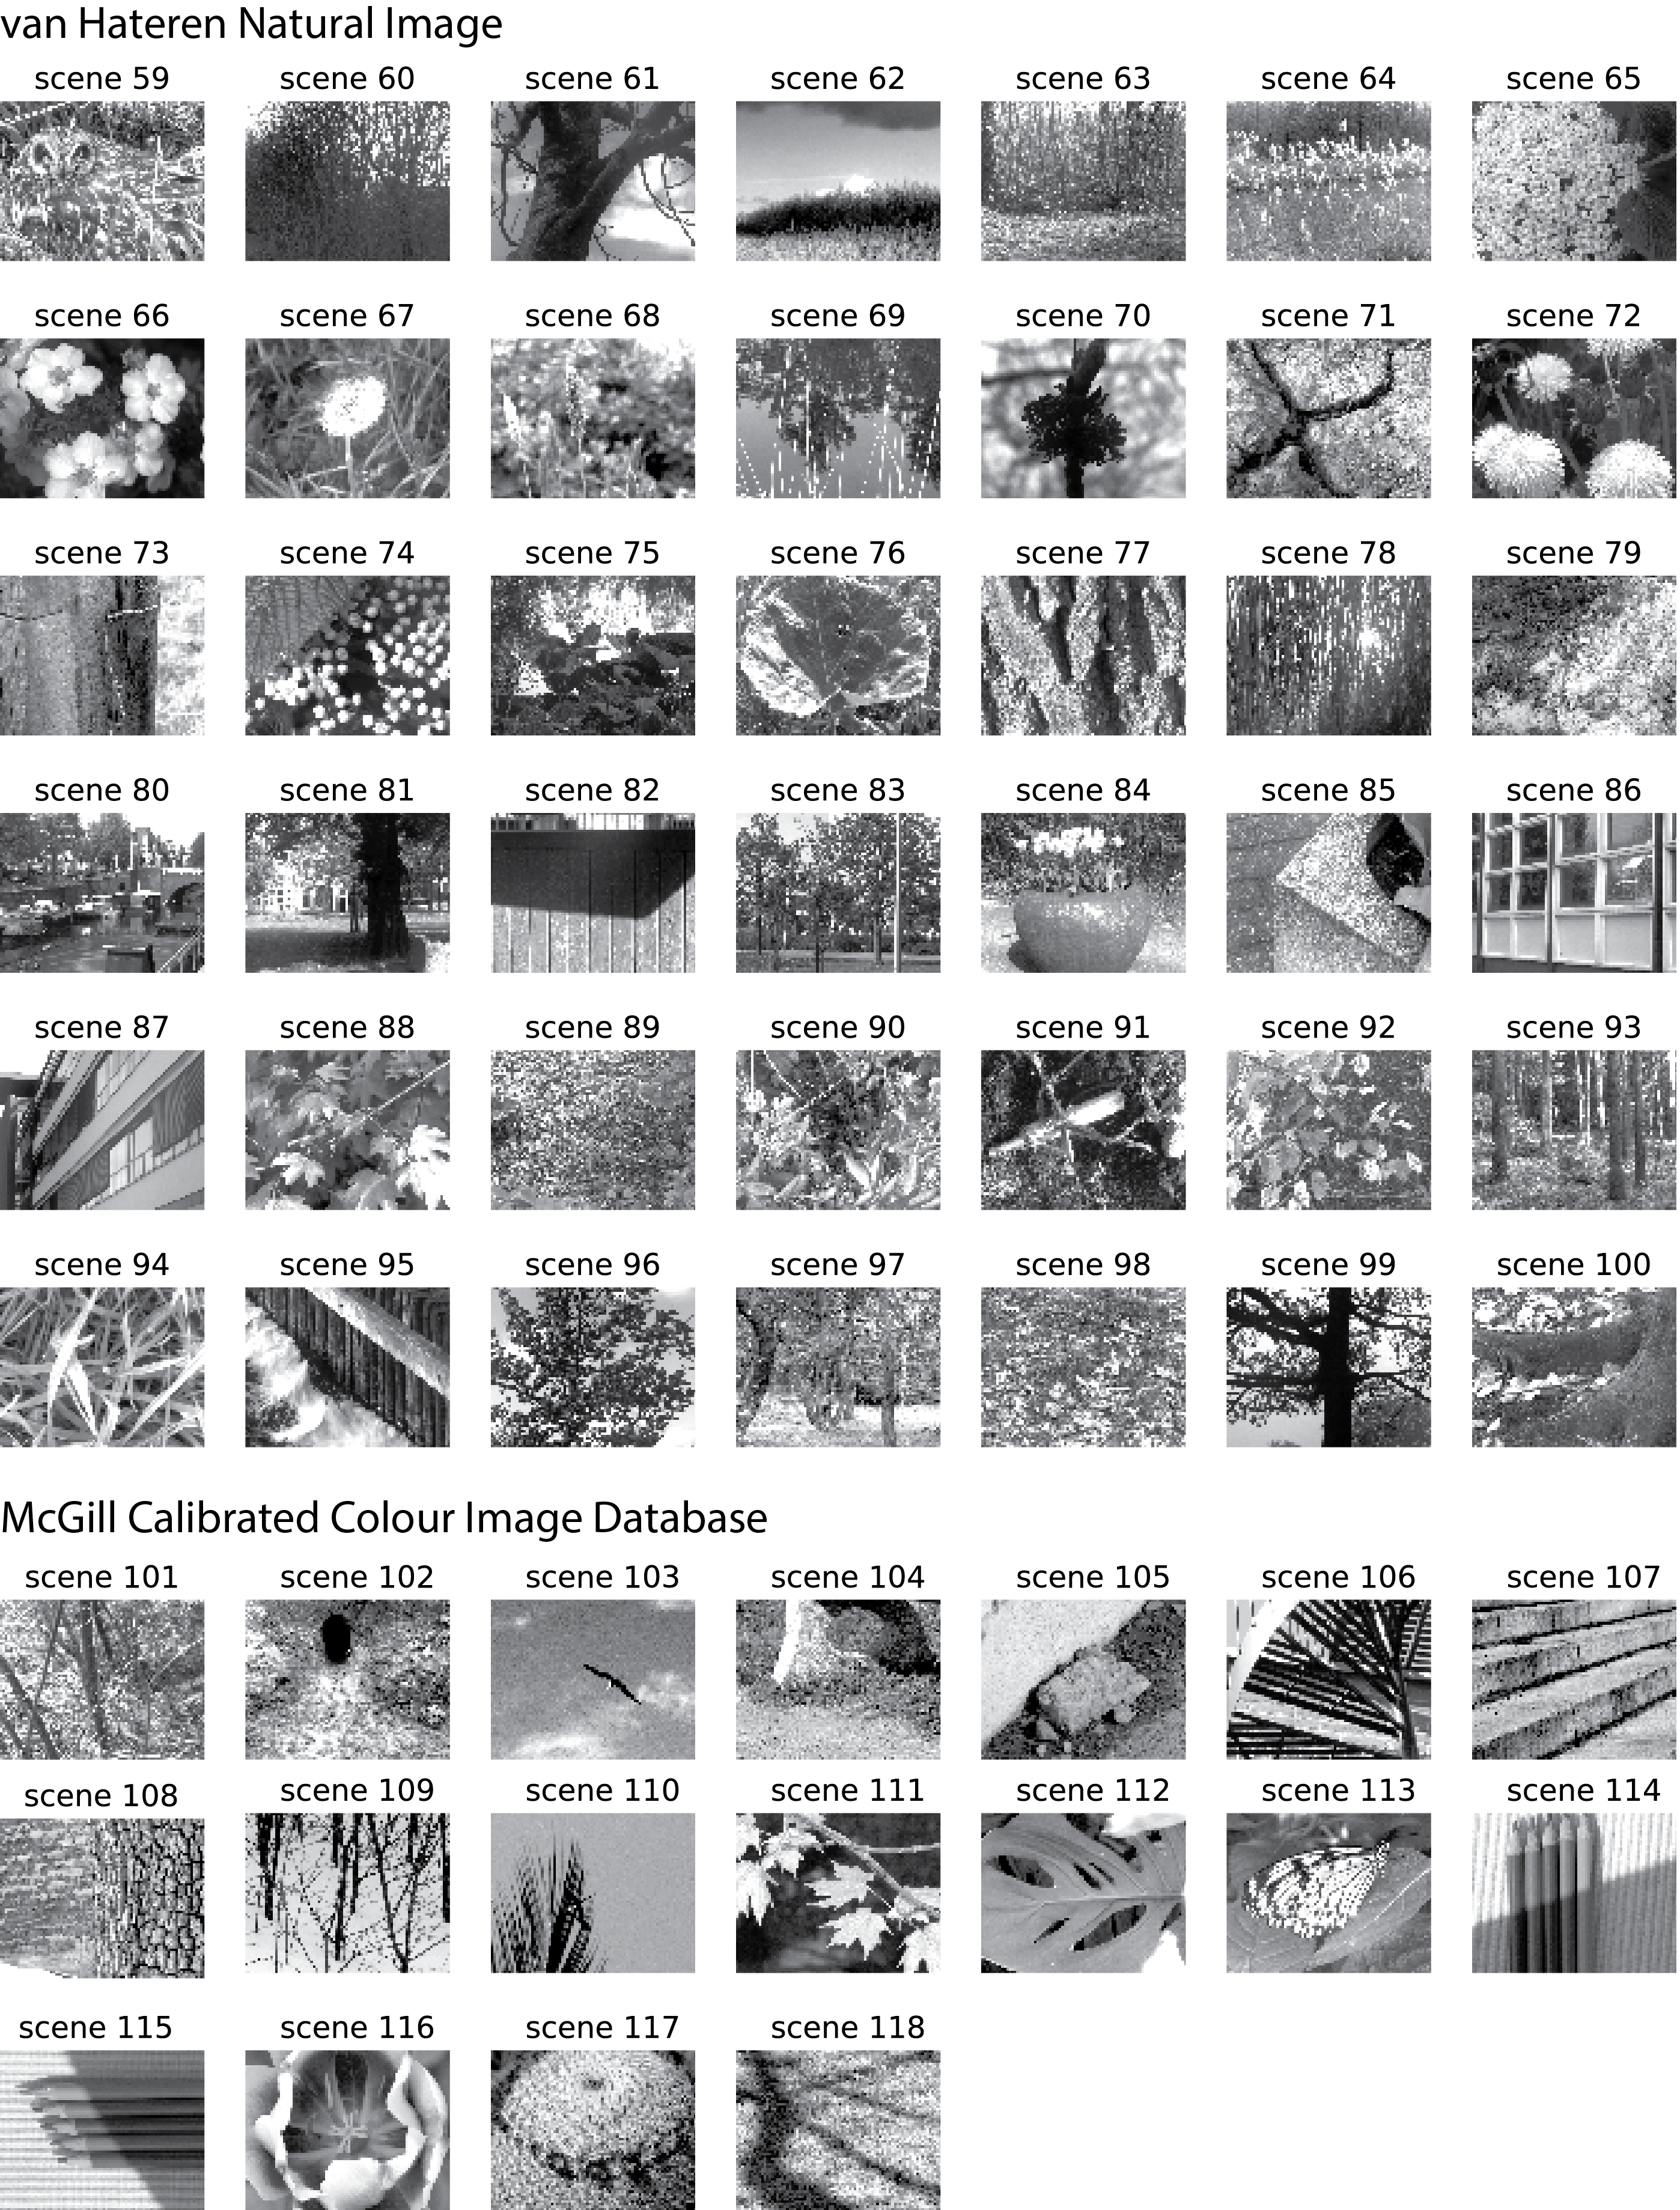
\includegraphics[width=\textwidth,height=0.9\textheight,keepaspectratio]{Figures/chapter5/images_dataset2.png}
  \caption[Thumbnail of Natural Images Stimulus Set - Part 2]{\textbf{Thumbnail of Natural Images Stimulus Set - Part 2} }
   \label{fig:images2}
\end{figure}
%-----------------------------------------------------------------------------
\section{Data and Methods for Analysis}
The dataset used for the analyses in this chapter was obtained from the Allen Brain Observatory public dataset (\url{http://observatory.brain-map.org/visualcoding/} and \textcite{Hawrylycz2016}). The dataset consists of neural responses from over 27,000 cells across four secondary visual areas and multiple cortical layers. Neural responses were recorded from mice passively viewing numerous visual stimuli, including static and drifting gratings, sparse noise, natural scenes, and natural movies. In particular, I analyzed data from the natural scenes sessions. 

Mice were presented with a total of 118 natural scenes (Figures \ref{fig:images1} and \ref{fig:images2}). Full screen images (1174 x 918 pixels) were presented in gray scale, matched for luminance, and contrast normalized. The images were obtained from public image databases: Berkeley Segmentation Dataset \parencite{Martin2001}, van Hateren Natural Image Dataset \parencite{VanHateren1998}, and the McGill Calibrated Colour Image Database \parencite{Olmos2004}. Each scene was presented for 250 ms and repeated 50 times, randomly. The images were presented consecutively, without an inter-stimulus interval. A blank screen was presented after ever 100 scenes. 

For each visual area, the data was organized into a matrix \emph{XT}, of size \emph{n} x \emph{c} x \emph{t}, where n = number of trials, c = number of cells in a visual area (or cell type), and t = time (or imaging frames).  Each cell had a total of 5900 trials (118 images, 50 repeats each). Blank stimulus trials were excluded in the analysis. The number of cells per area ranged between 2157 (area PM) to 4189 (V1) (Table \ref{celltable}). The data was acquired at approximately 31 frames per second and thus approximately 7 imaging frames were acquired per 250ms of stimulus presentation. Included in \emph{XT} was the pre-stimulus and post-stimulus response, each 250 ms in length. The analyses in this project were done using the relative changes in fluorescence ($\Delta$ F/F) as the neuronal response rather than inferred spike events.
%-----------------------------------------------------------------------------
%-----------------------------------------------------------------------------
\begin{table}
\centering
\begin{tabular}{@{}ccccc@{}}
\toprule
\begin{tabular}[c]{@{}c@{}}Layers\\ (Cre line)\end{tabular} & PM   & AL   & LM   & V1   \\ \midrule
\begin{tabular}[c]{@{}c@{}}2/3\\ (Cux-cre)\end{tabular}    & 1646 & 1380 & 1580 & 2802 \\
\begin{tabular}[c]{@{}c@{}}4\\ (Rorb-cre)\end{tabular}     & 208  & 480  & 530  & 821  \\
\begin{tabular}[c]{@{}c@{}}5\\ (Rbp4-cre)\end{tabular}     & 303  & 463  & 496  & 566  \\ \bottomrule
\begin{tabular}[c]{@{}c@{}}Total cells\end{tabular}        & 2157  & 2323  & 2606  & 4189  \\
\end{tabular}
\caption{Cells per Layer per Visual Area}
\label{celltable}
\end{table}
%-----------------------------------------------------------------------------
%-----------------------------------------------------------------------------

To measure performance on identifying natural scenes given a neural activity pattern, I trained a linear support vector classifier (SVM, one-vs-rest classifier scheme) on the average response during 200-300ms post stimulus onset, and computed cross-validated test accuracy for the trained classifier for each area. The classifier was trained on 70\% of the trials in an area, and tested on the remaining 30\%. In most cases I repeated this procedure 10 times to obtain an average and standard error of the mean (SEM). The SVM linear classifier procedure is similar to the approach used in previous studies in primate visual object recognition \parencite{Hung2005,Rust2010a}
%-----------------------------------------------------------------------------
%-----------------------------------------------------------------------------
\section{Results}
\subsection{Decoding Natural Scene Identity}
The first task was to decode the identity of natural scenes given the population activity from each area. All the visual areas performed well above chance level (0.85\%) on the identity task (Figure \ref{fig:decodebar} a). Primary visual cortex (V1) exhibited the highest performance (>75\%) on linearly classifying the natural images, followed by area LM (>50\%). Area LM is an anatomical equivalent of primate V2 because it is the most prominent recipient of V1 projections and LM projects to all visual areas \parencite{Wang2012}. LM and AL have also been referred to as the gateways into the putative mouse ventral and dorsal processing streams based on evidence from cytoarchitecture and anatomical projections \parencite{wang2011,Wang2013a}.  Areas AL and PM performed similarly (> 30\%). To make sure that the performance accuracy of V1 was not merely due to uneven total number of neurons across visual areas, I repeated the decoding image identity task with 2100 neurons from each areas. As shown in Figure \ref{fig:decodebar}b, the trend in performance accuracy across areas remains; however the overall accuracy is decreased for each area. This is consistent with the observation that performance accuracy increases with the size of the population for each area (Figure \ref{fig:decodepop}).\par 
%-----------------------------------------------------------------------------
\begin{figure}
  \centering
    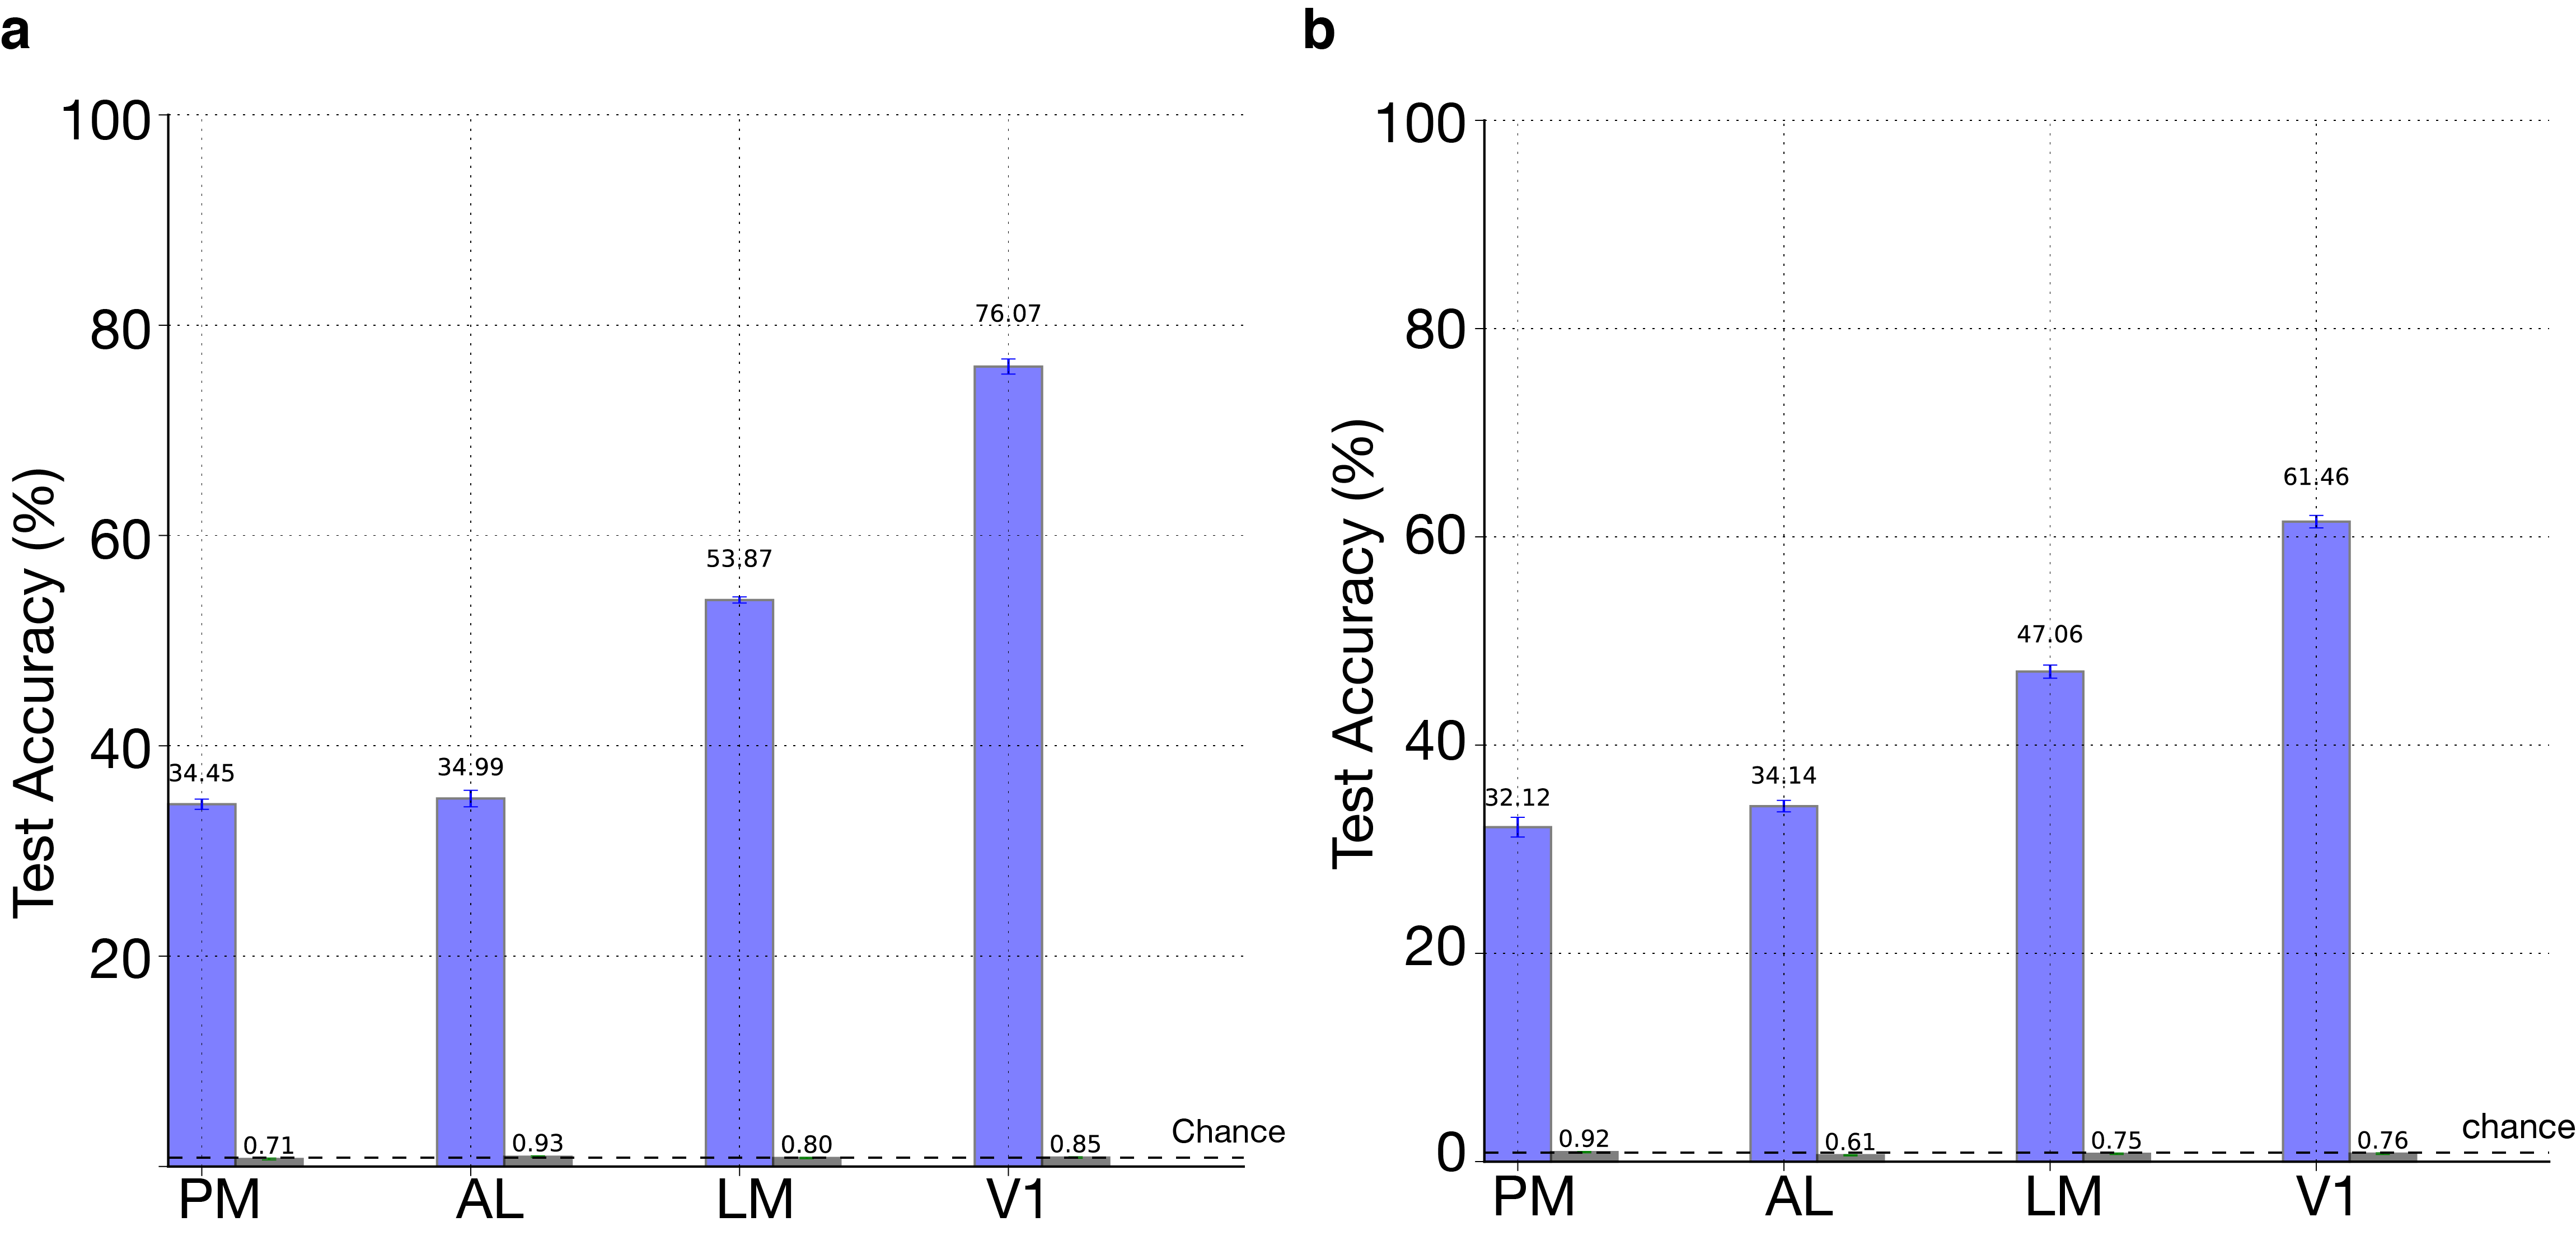
\includegraphics[width=\textwidth]{Figures/chapter5/accuracy_all_and_2100_neurons.png}
%   	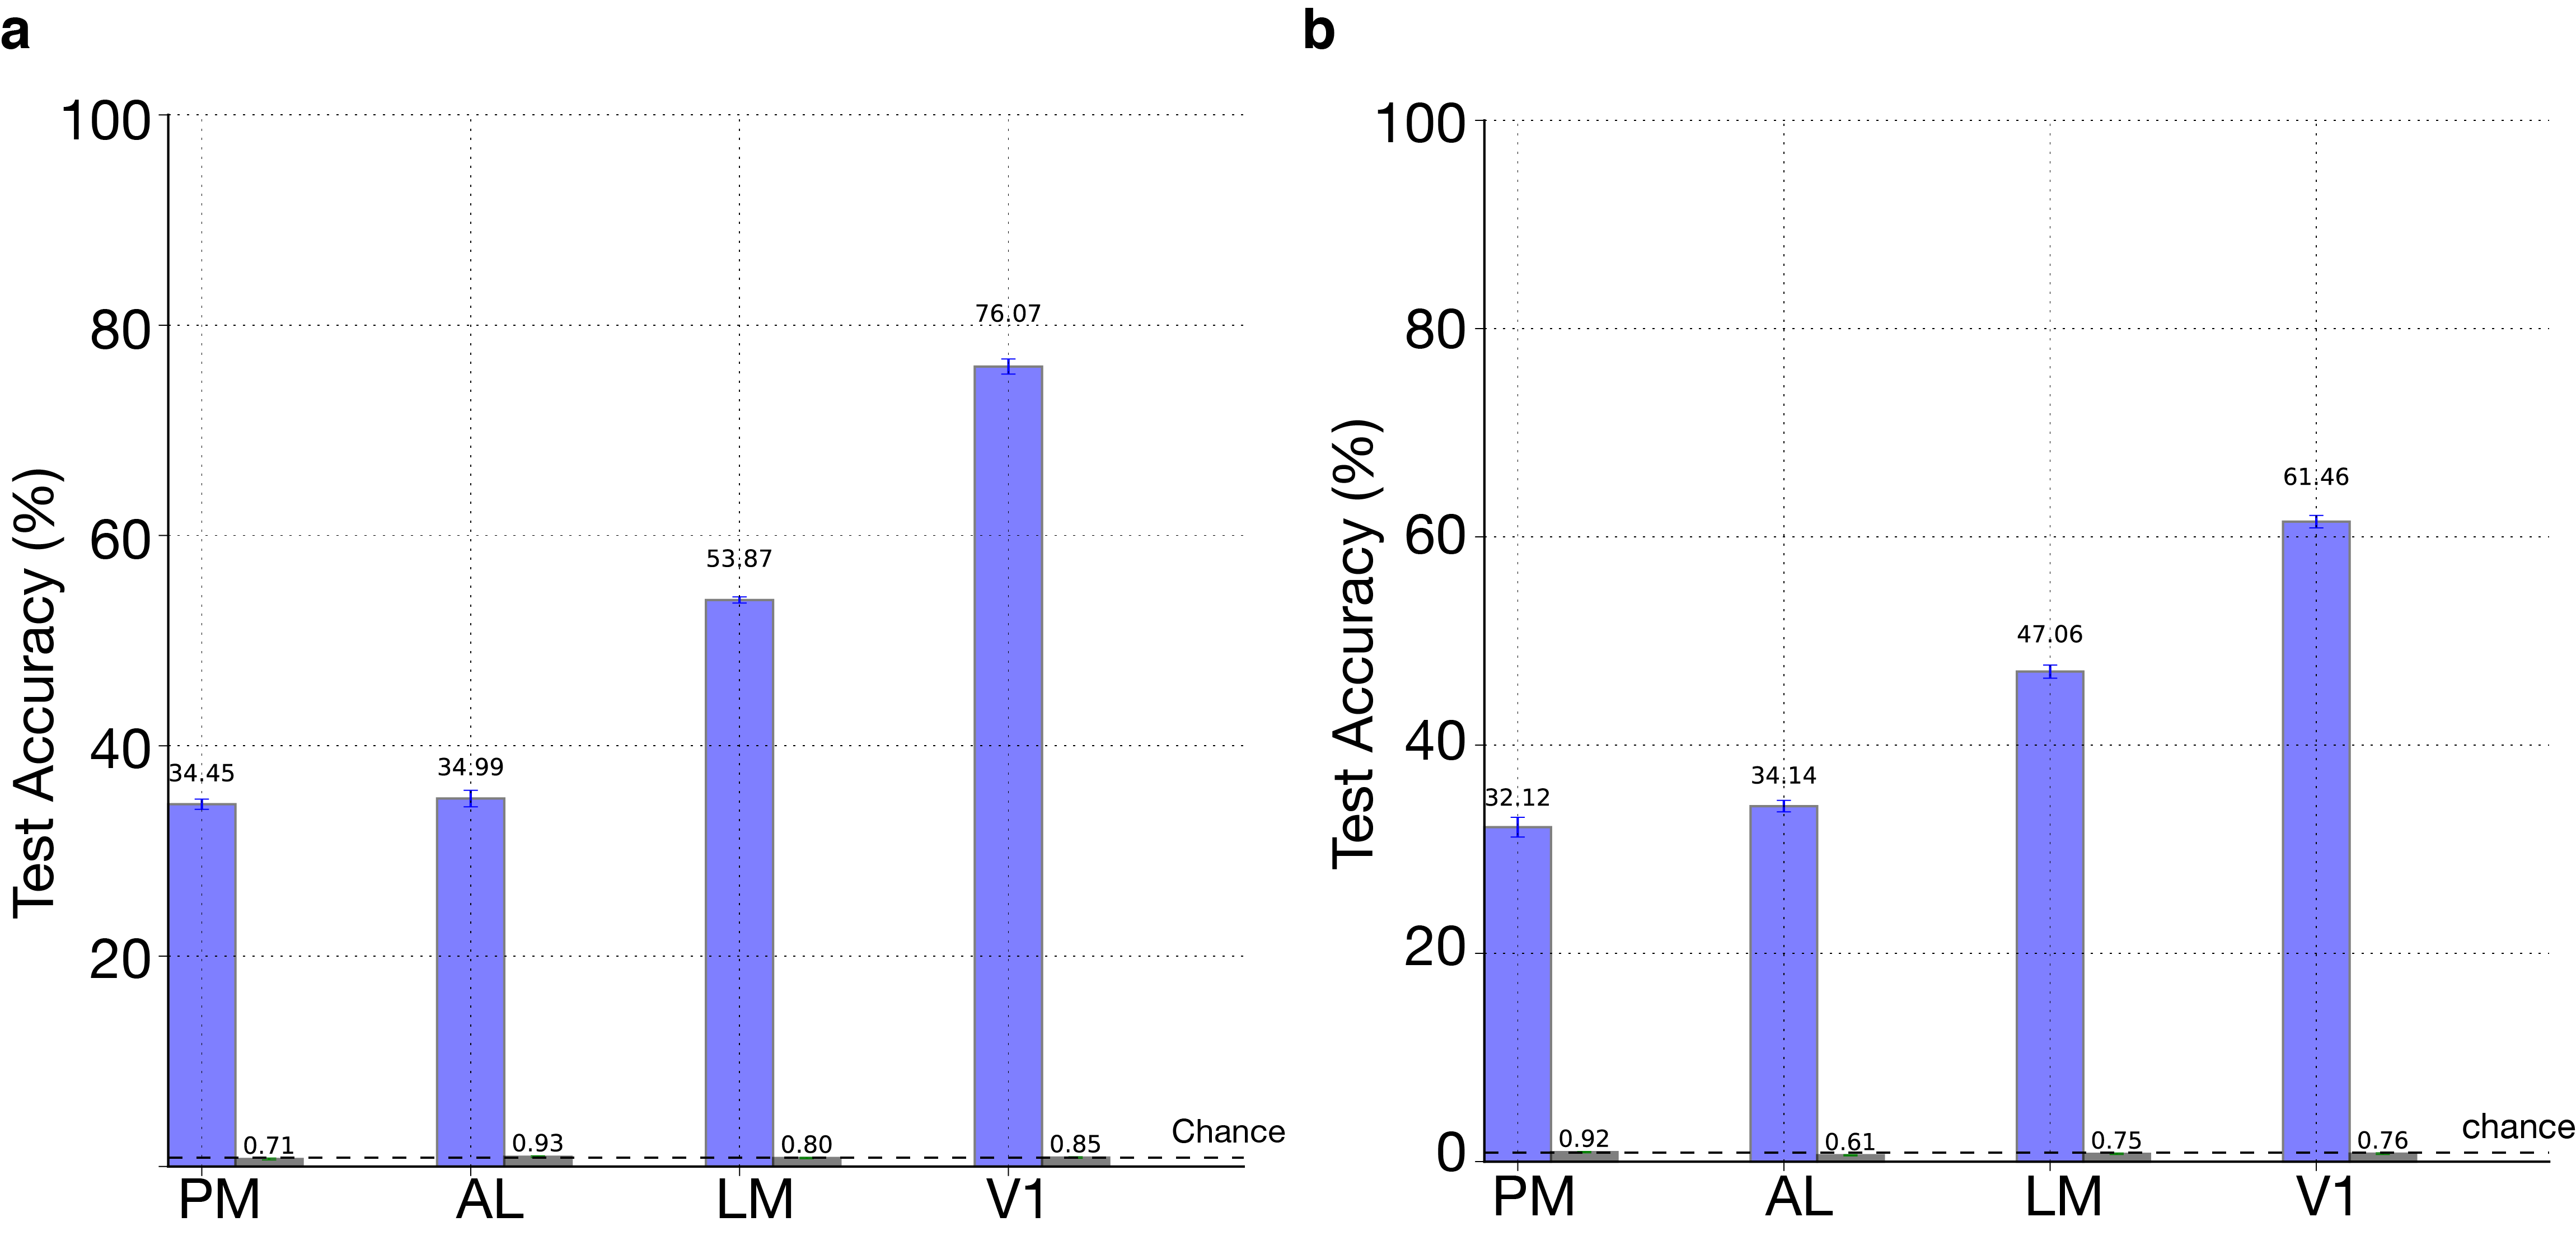
\includegraphics[scale=0.35]{Figures/chapter5/accuracy_all_and_2100_neurons.png}
    \caption[Decoder Test Accuracy]{\textbf{Decoder Test Accuracy} (a) including all neurons per visual area and (b) including a subset of 2100 neurons per visual area. Purple bars represent decoder test accuracy. Gray bars represent shuffled label controls. Error bars represent standard error of the mean.}
  \label{fig:decodebar}
\end{figure}
%-----------------------------------------------------------------------------
\begin{figure}
  \centering
    	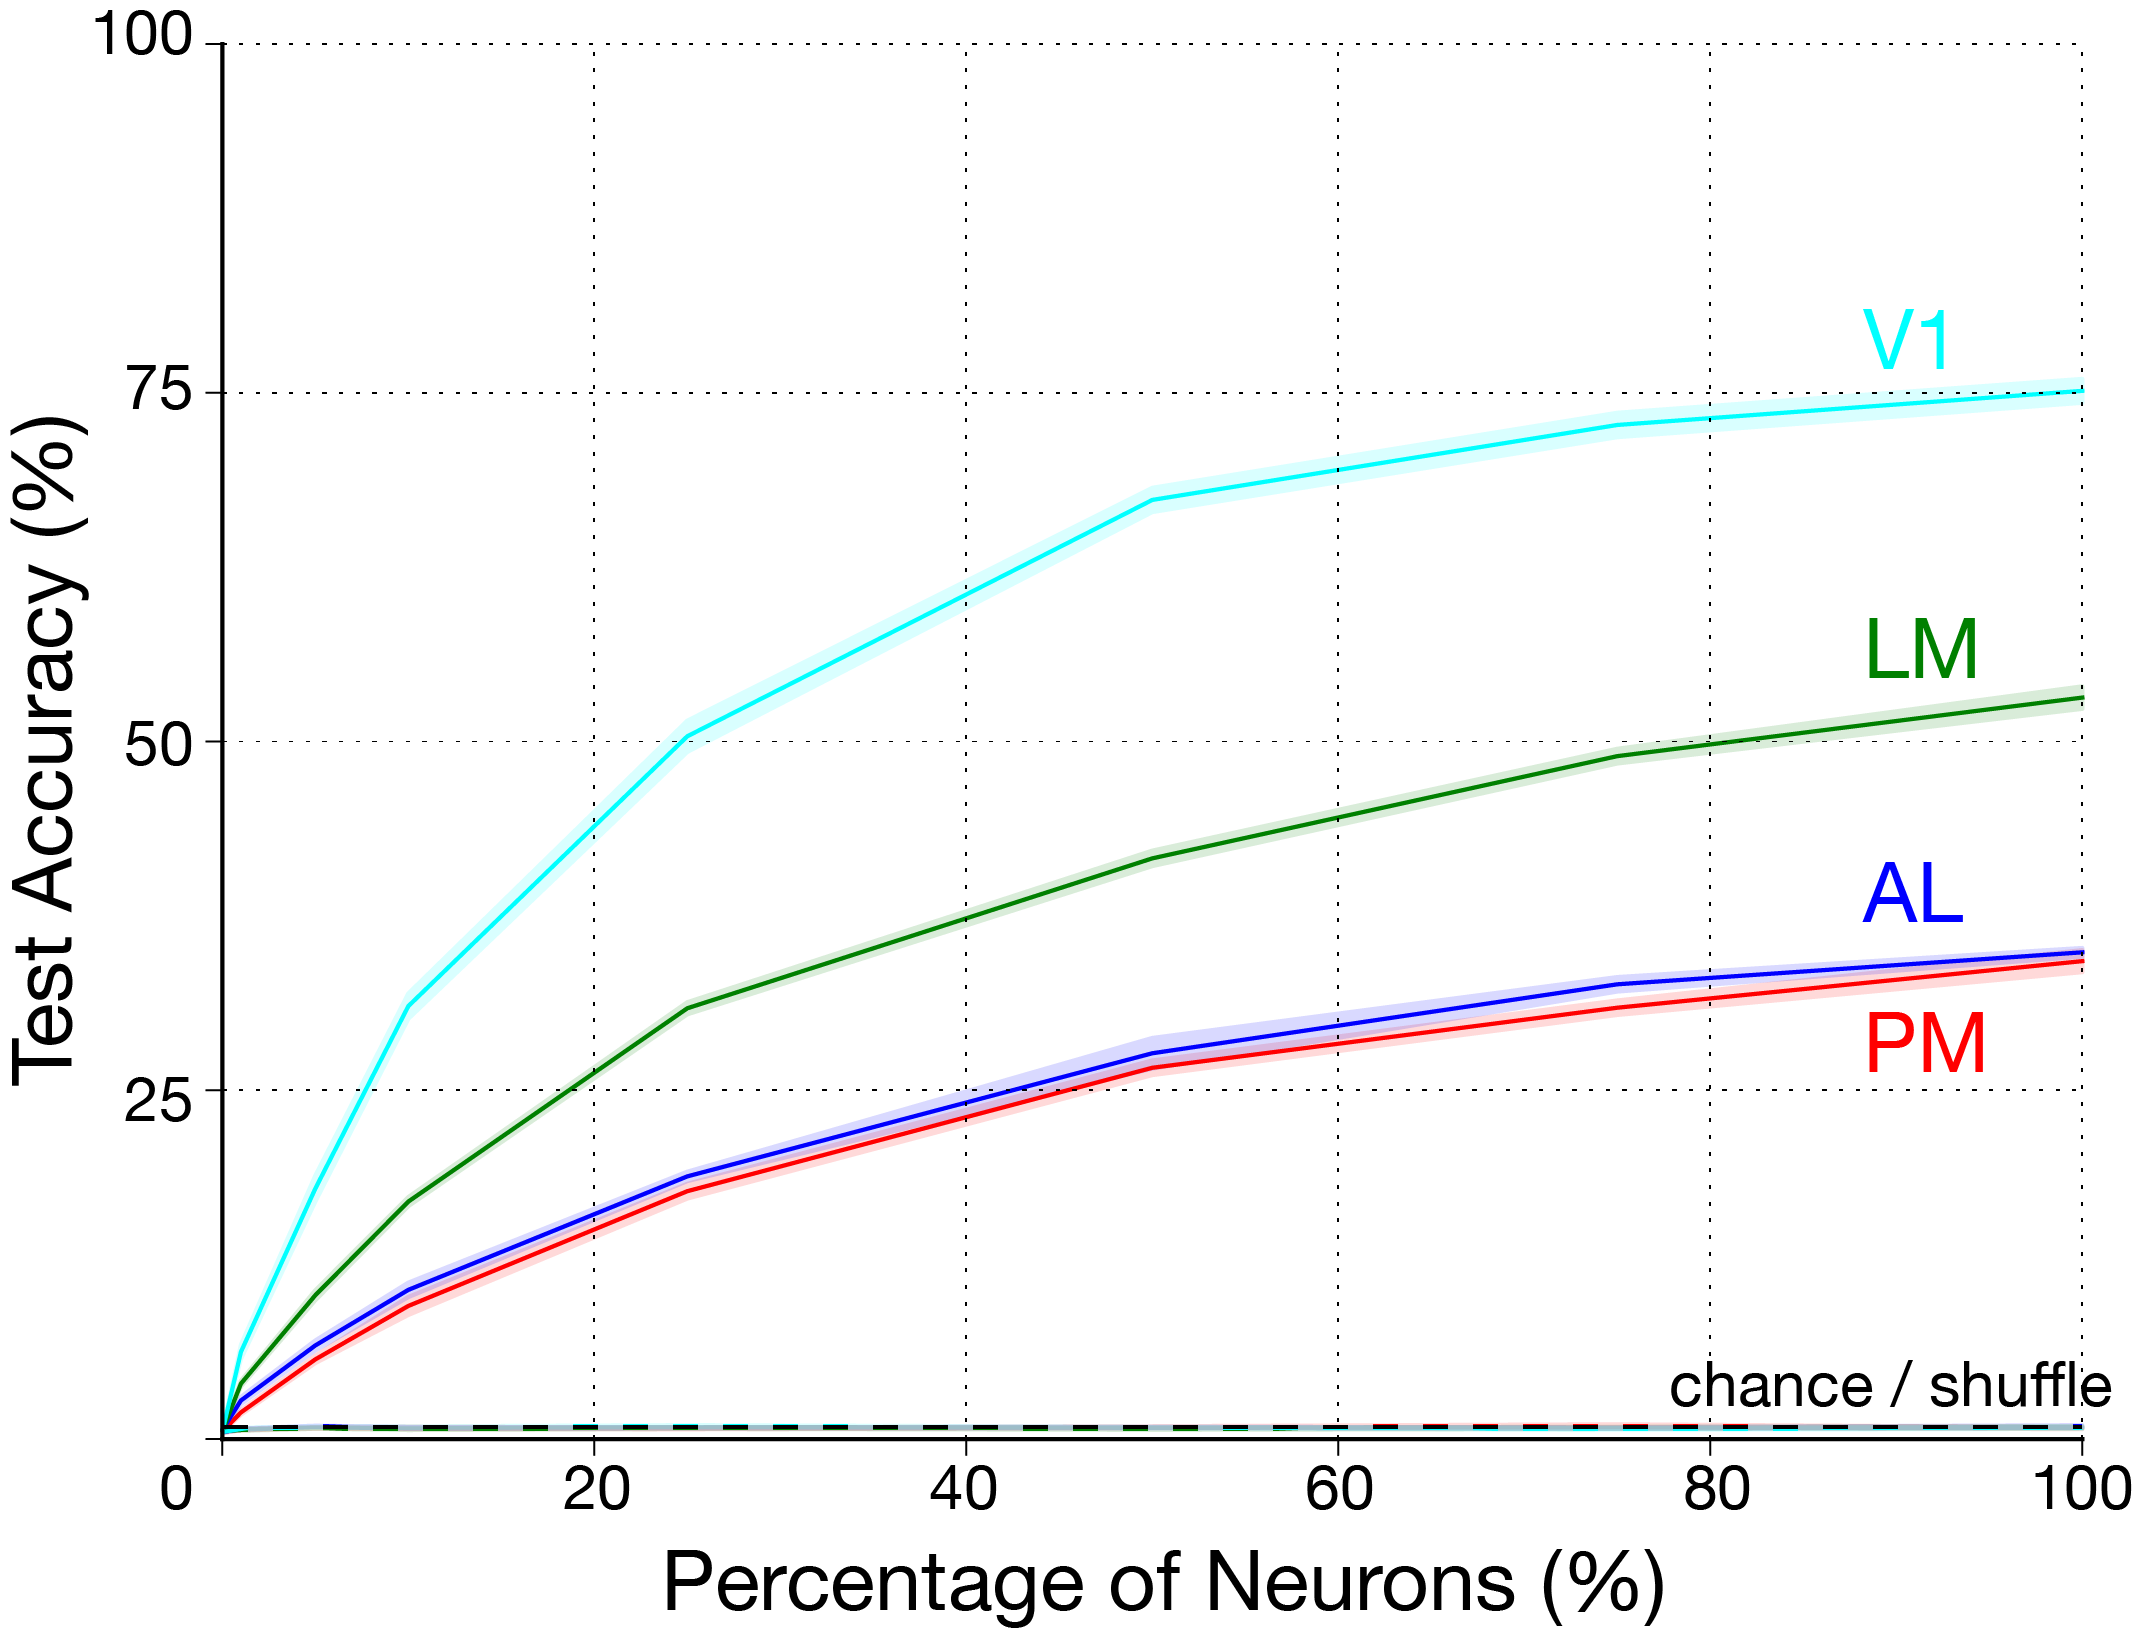
\includegraphics[width=\textwidth]{Figures/chapter5/accuracy_population.png}
%   	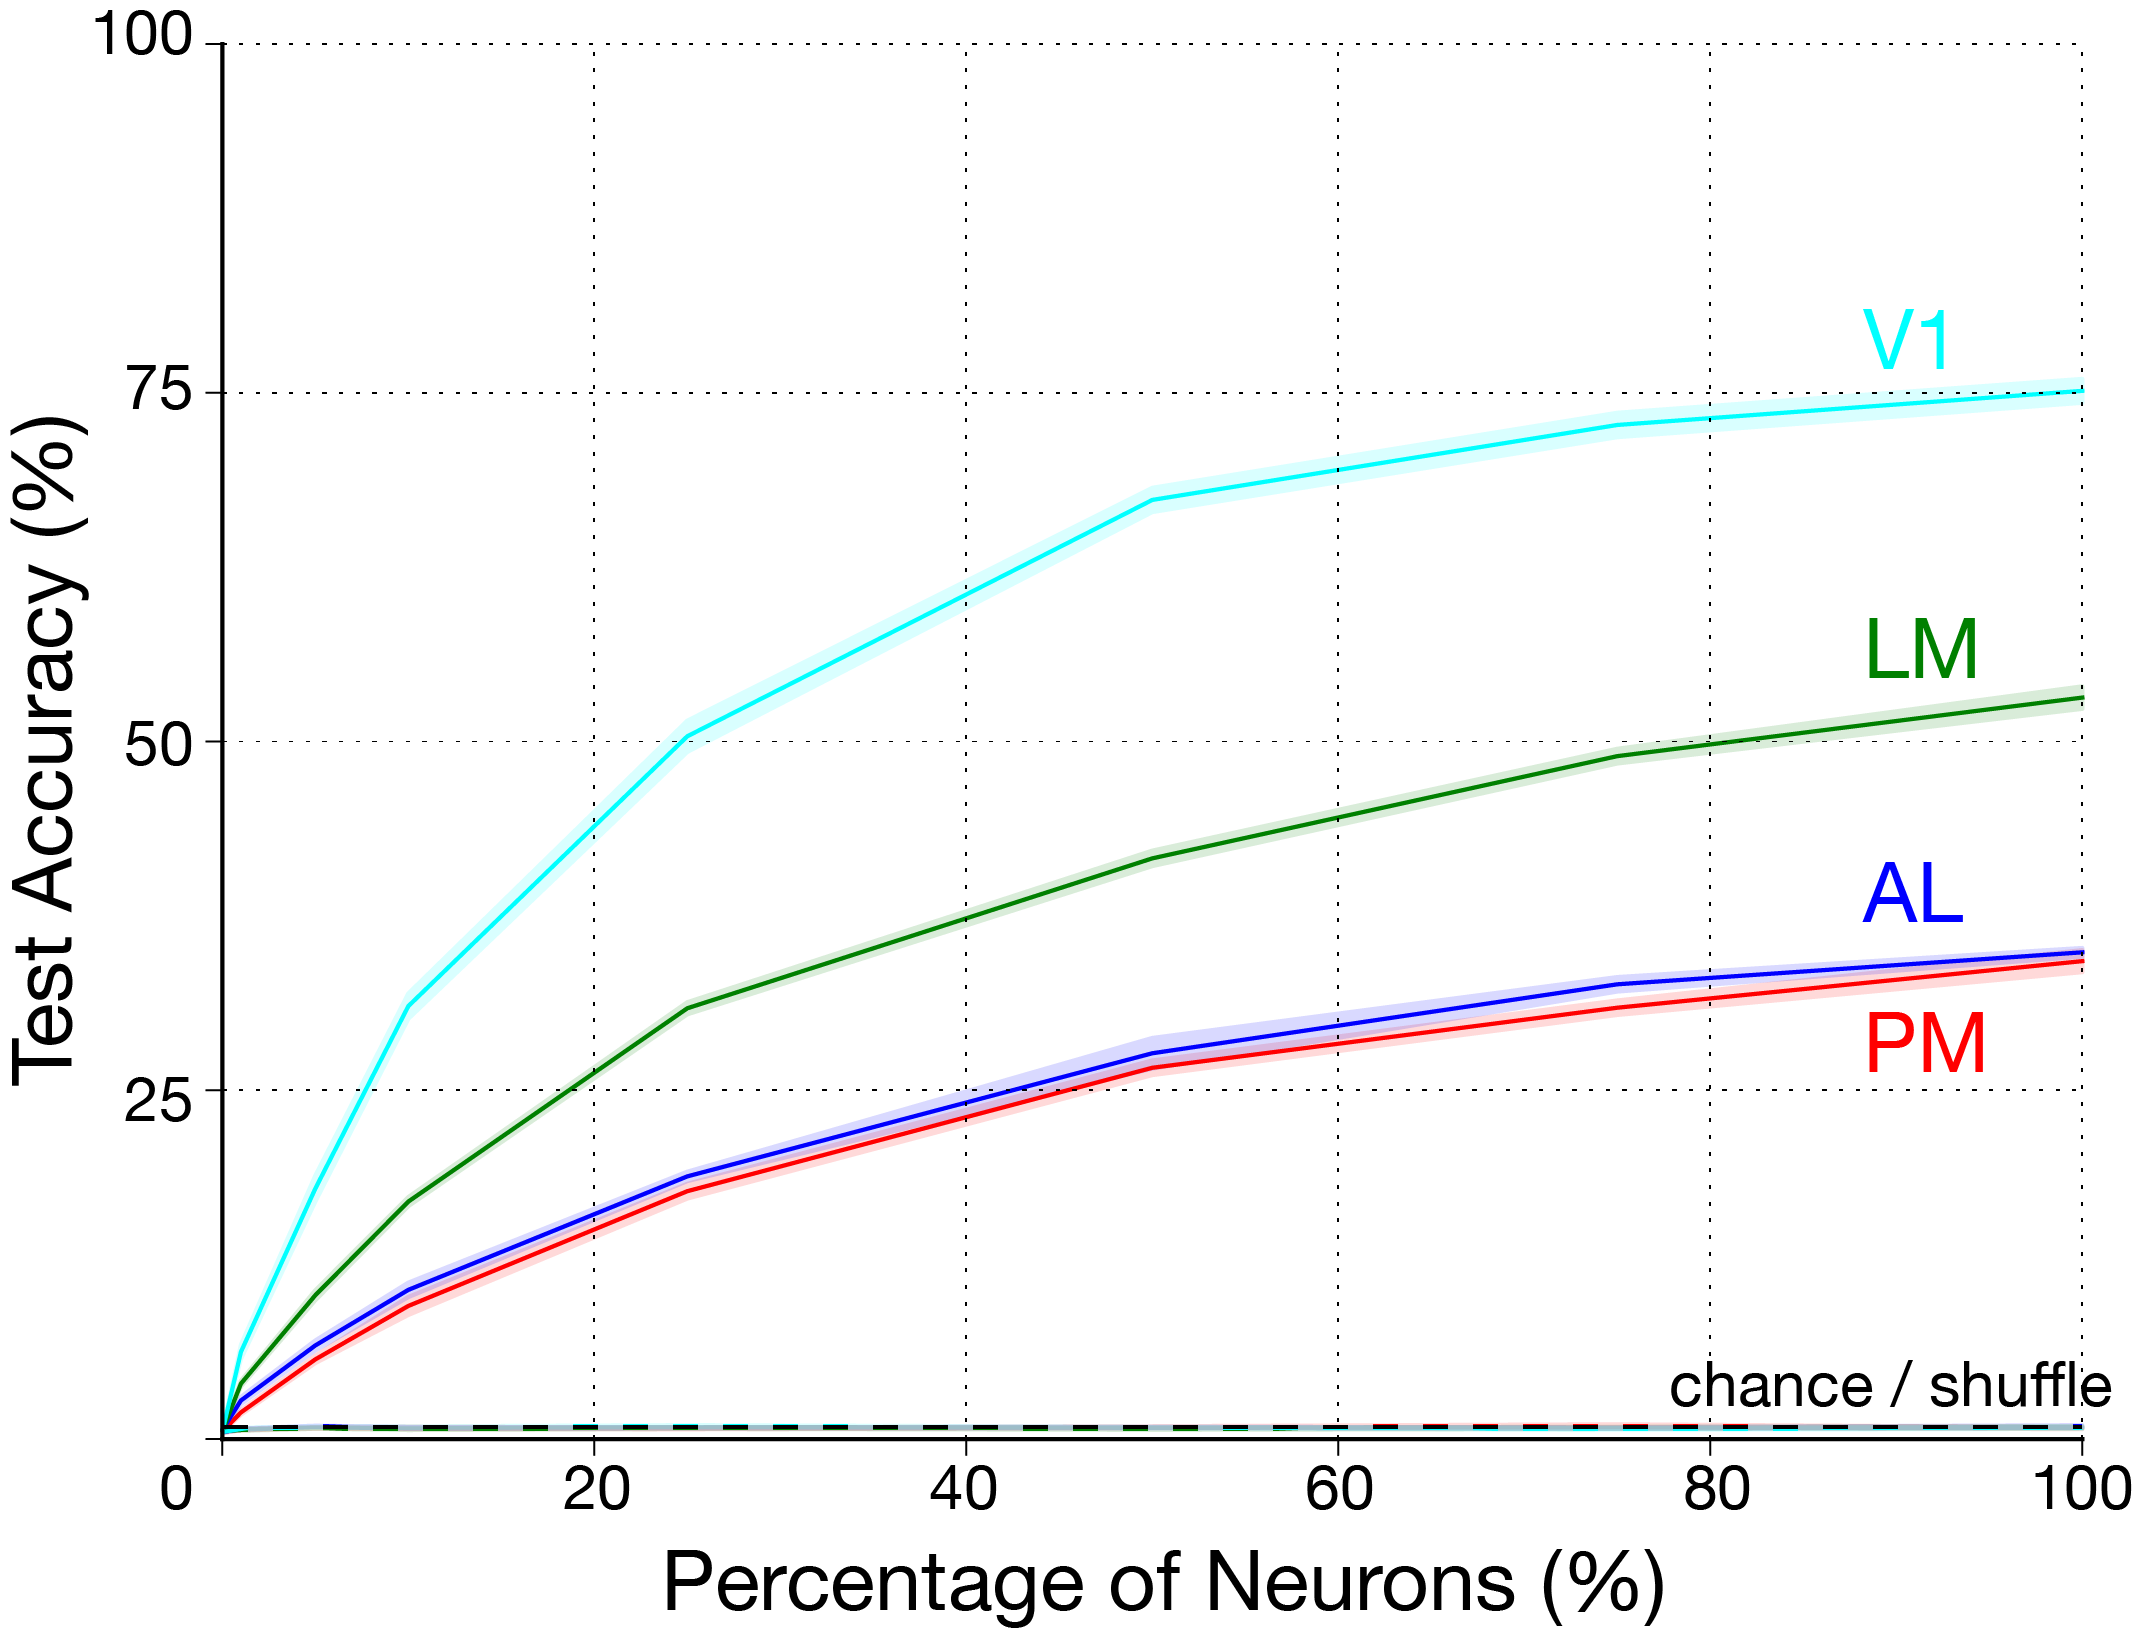
\includegraphics[scale=0.45]{Figures/chapter5/accuracy_population.png}
    \caption[Decoder Accuracy Per Visual Area Population Size]{\textbf{Decoder Accuracy Per Visual Area Population Size}. Test accuracy increases with number of neurons for each visual area. Solid line represents test accuracy. Shaded error bars represent standard error of the mean.}
  \label{fig:decodepop}
\end{figure}
%-----------------------------------------------------------------------------
To evaluate and compare each classifier’s performance, I created a confusion matrix (Figure \ref{fig:confusion}), which compares the classifier’s predicted image identity label and the true image label. The confusion matrix shows the proportion of cases the classifier predicted the true image label, otherwise known as the conditional probability (\emph{P(predicted|true)}) of the classifier predicted label given the true label. The confusion matrix also shows which images elicit similar neural population responses. From the confusion matrix, I computed the mutual information (\emph{MI}) between the classifier's prediction and the true image label: 
\begin{equation}
\begin{aligned}
MI = \sum_{l} \sum_{l'} P(l',l) log_2 \frac{P(l',l)}{P(l')P(l)} \\
P(l) = \sum_{l} P(l',l) \\
P(l') = \sum_{l'} P(l',l)
\end{aligned}
\label{eq:mutualinfo}
\end{equation}
Where \emph{l} is the true image label, \emph{l'} is the predicted image label, \emph{P(l',l)} is the joint probability (normalized confusion matrix), \emph{P(l)} and \emph{P(l')} are the marginal probability distributions. Similar to the identity decode performance accuracy, the mutual information increases with the size of the population (Figure \ref{fig:mutualinfopop}).\par 
%-----------------------------------------------------------------------------
\begin{figure}
  \centering
     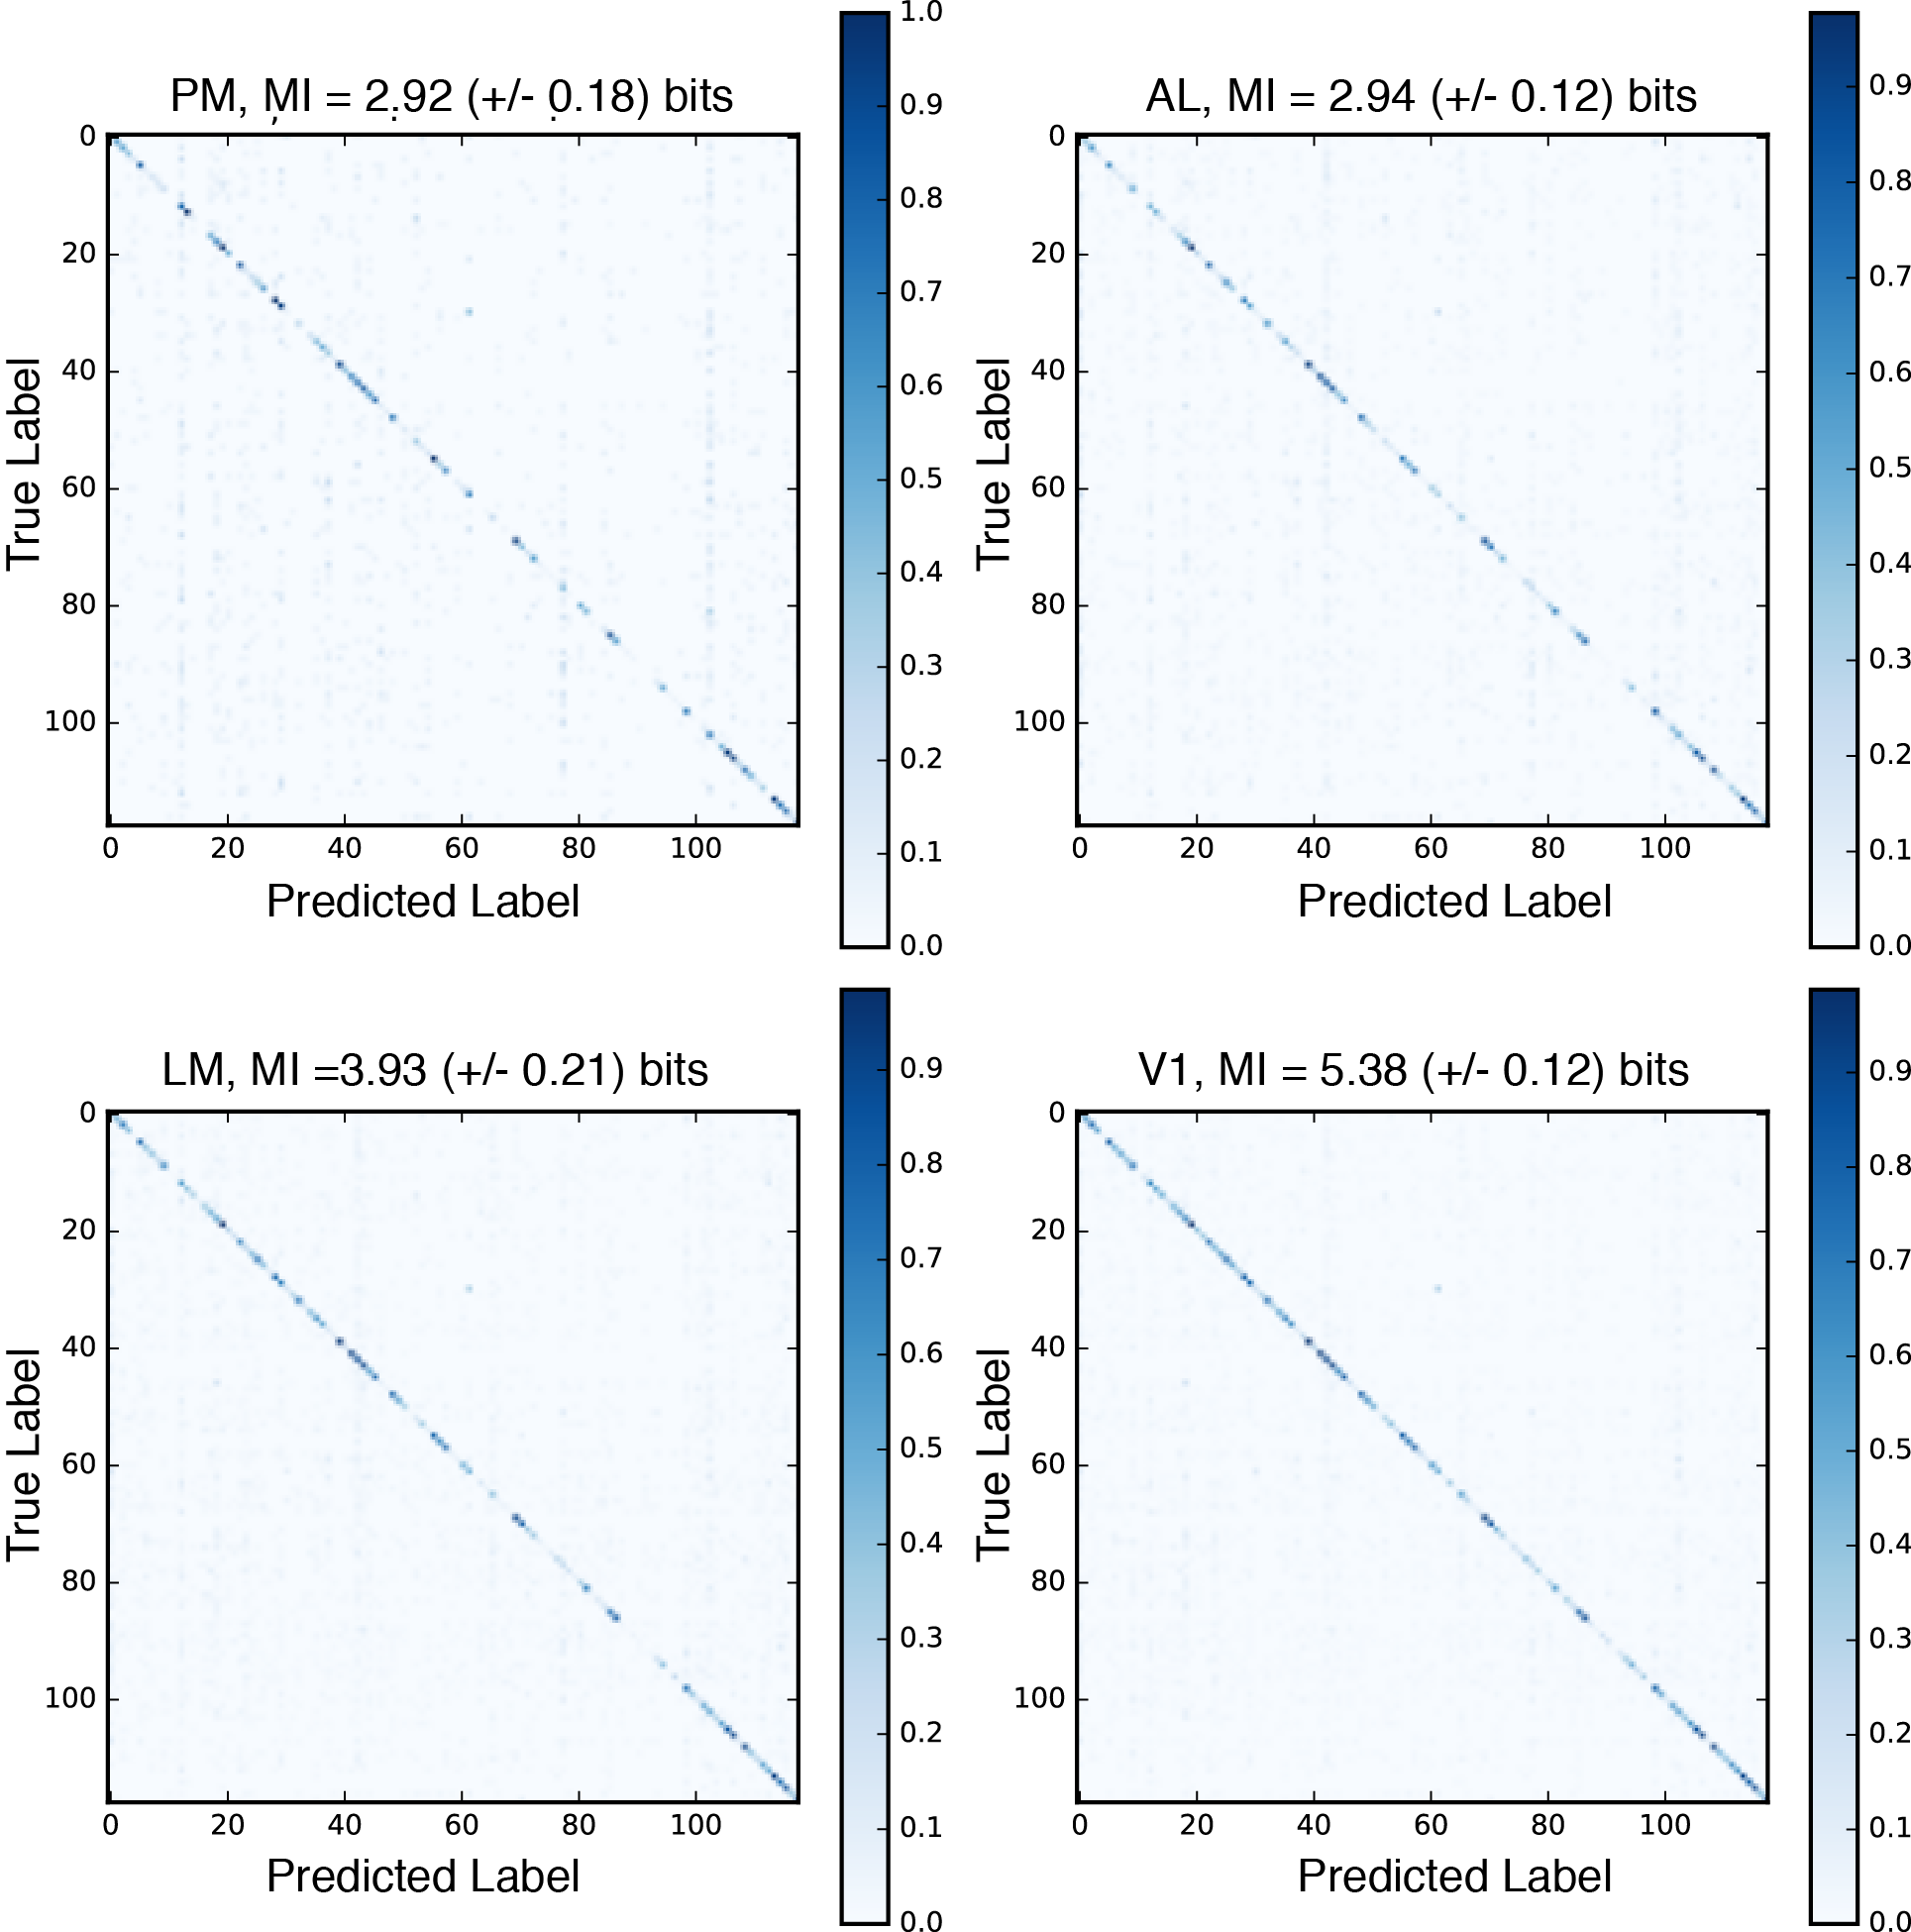
\includegraphics[width=\textwidth]{Figures/chapter5/confusion.png}
%    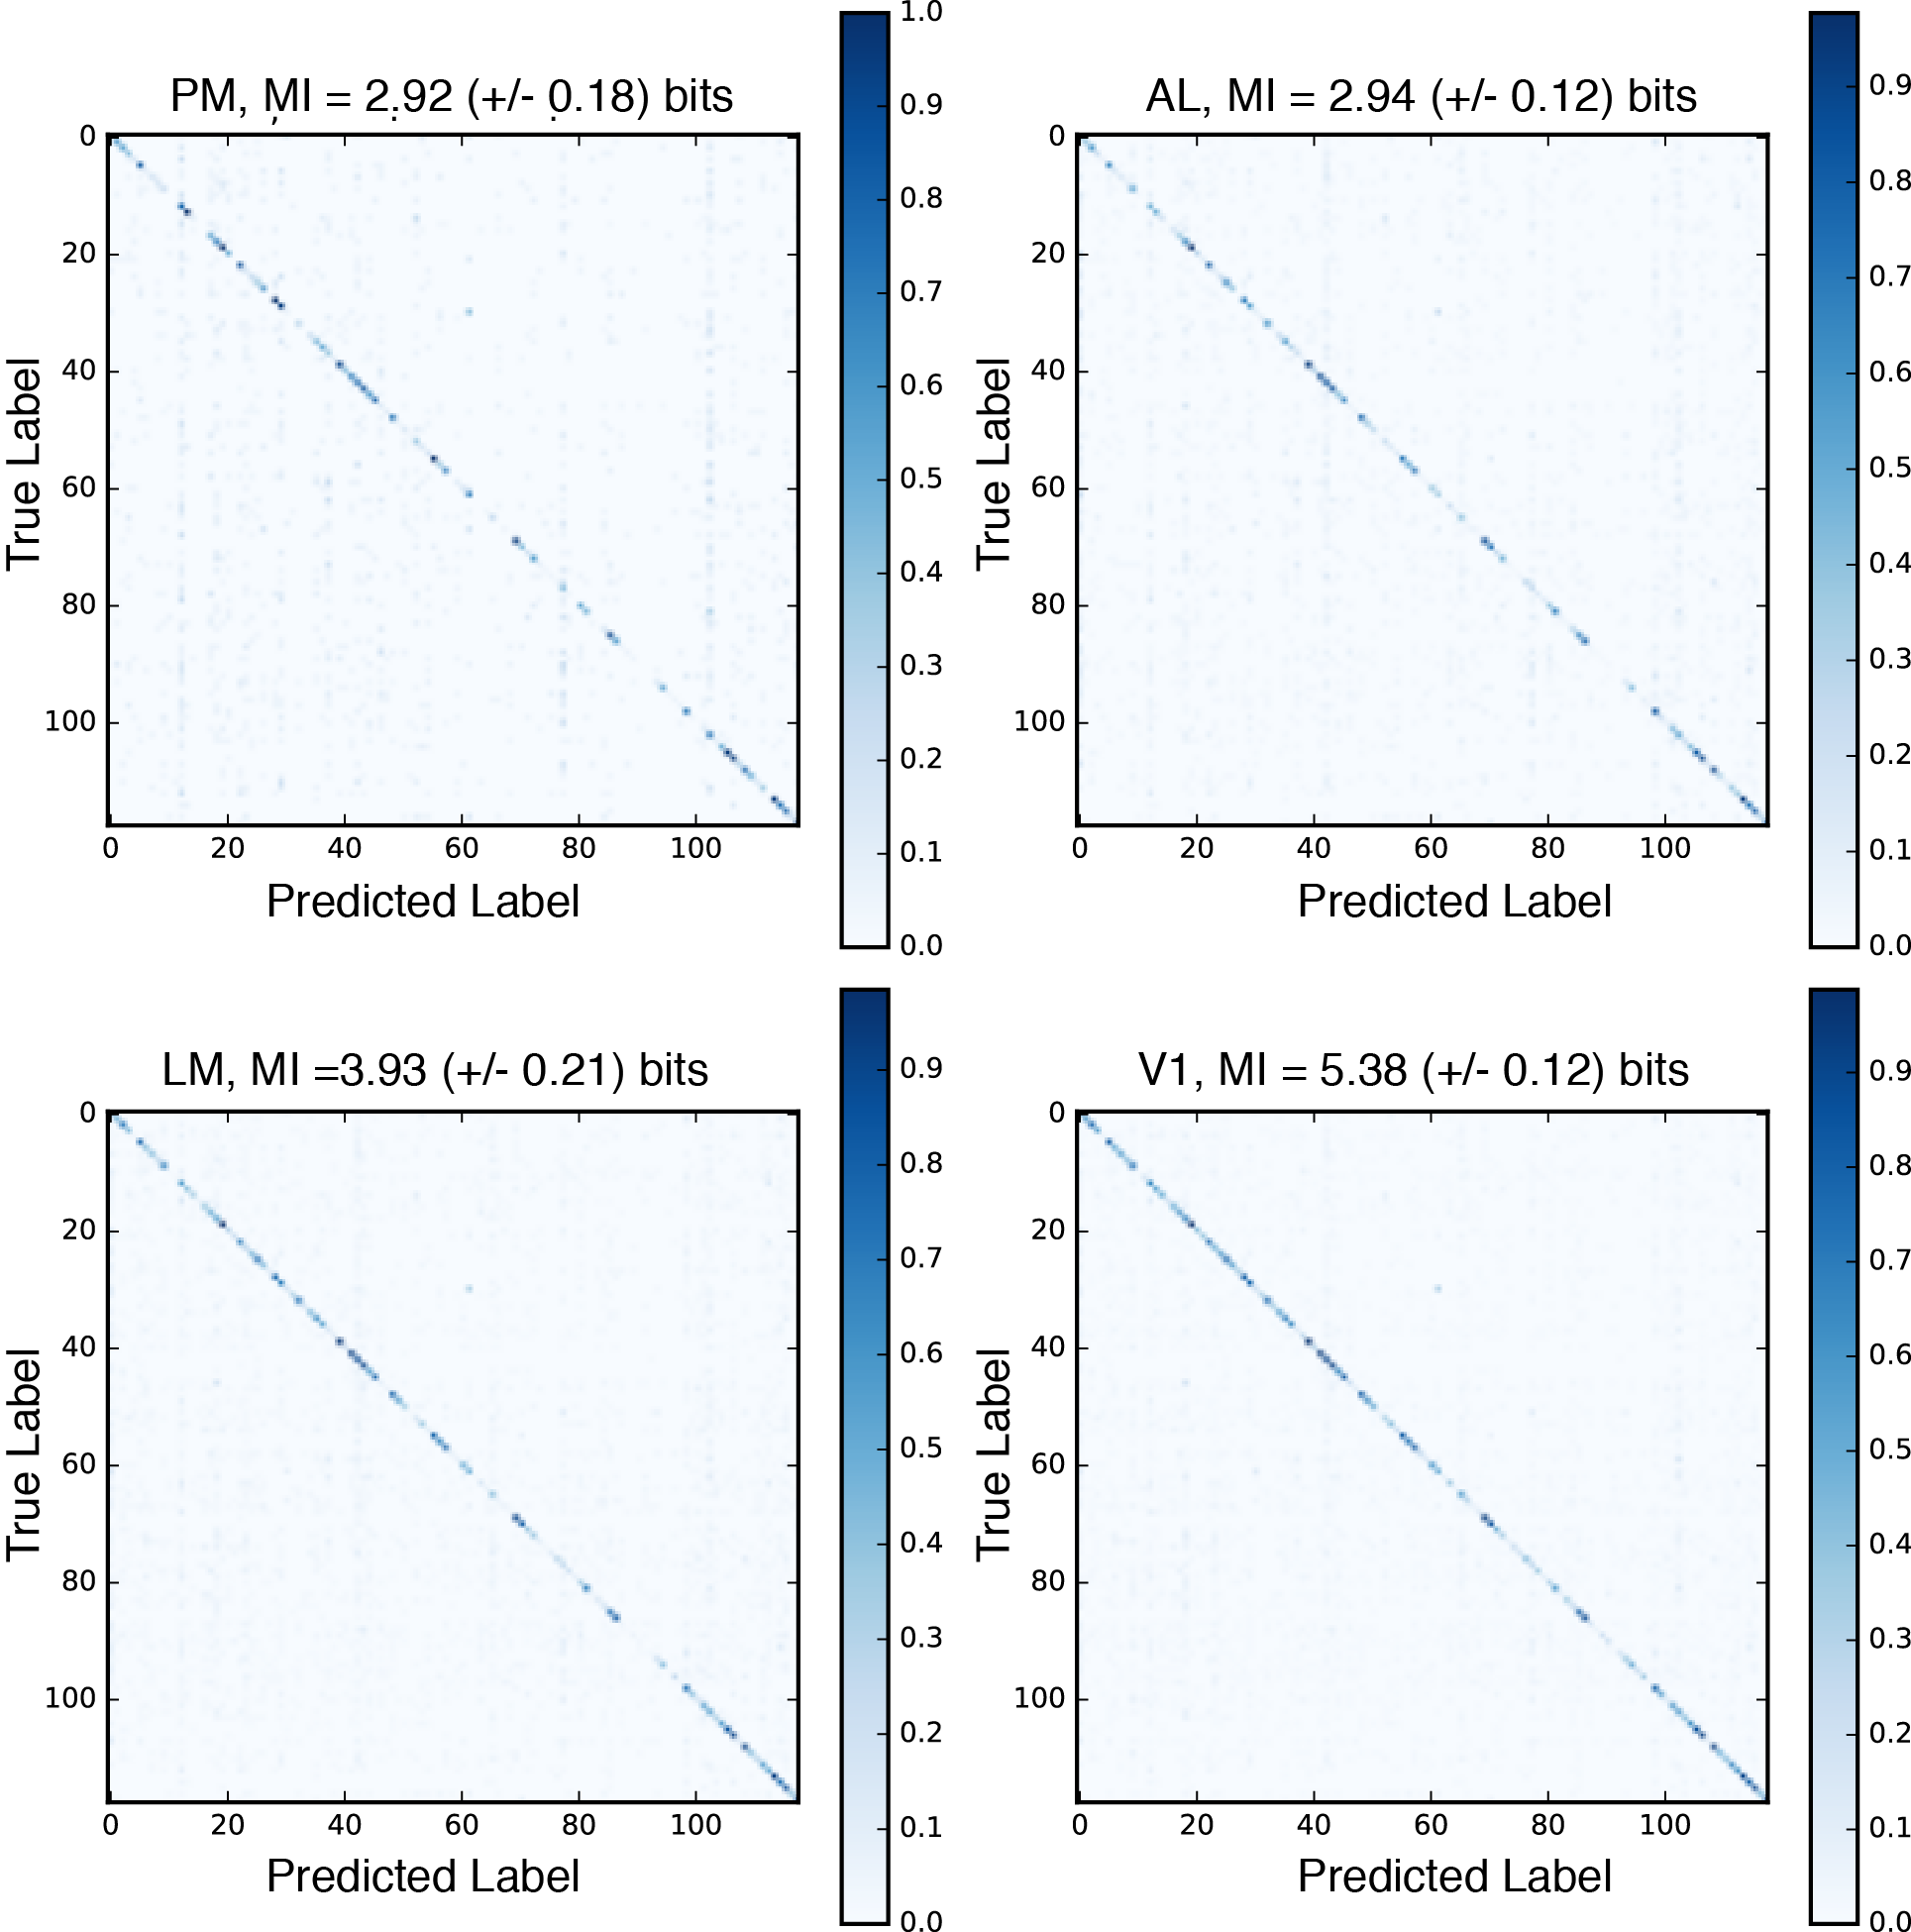
\includegraphics[scale=0.725]{Figures/chapter5/confusion.png}
  \caption[Confusion Matrix]{\textbf{Confusion Matrix} for each visual area compares decoder performance (or misclassification) for pairs of natural images. Mutual information (in bits) is reported for each confusion matrix +/- standard error of mean}
   \label{fig:confusion}
\end{figure}
%-----------------------------------------------------------------------------
\begin{figure}
  \centering
   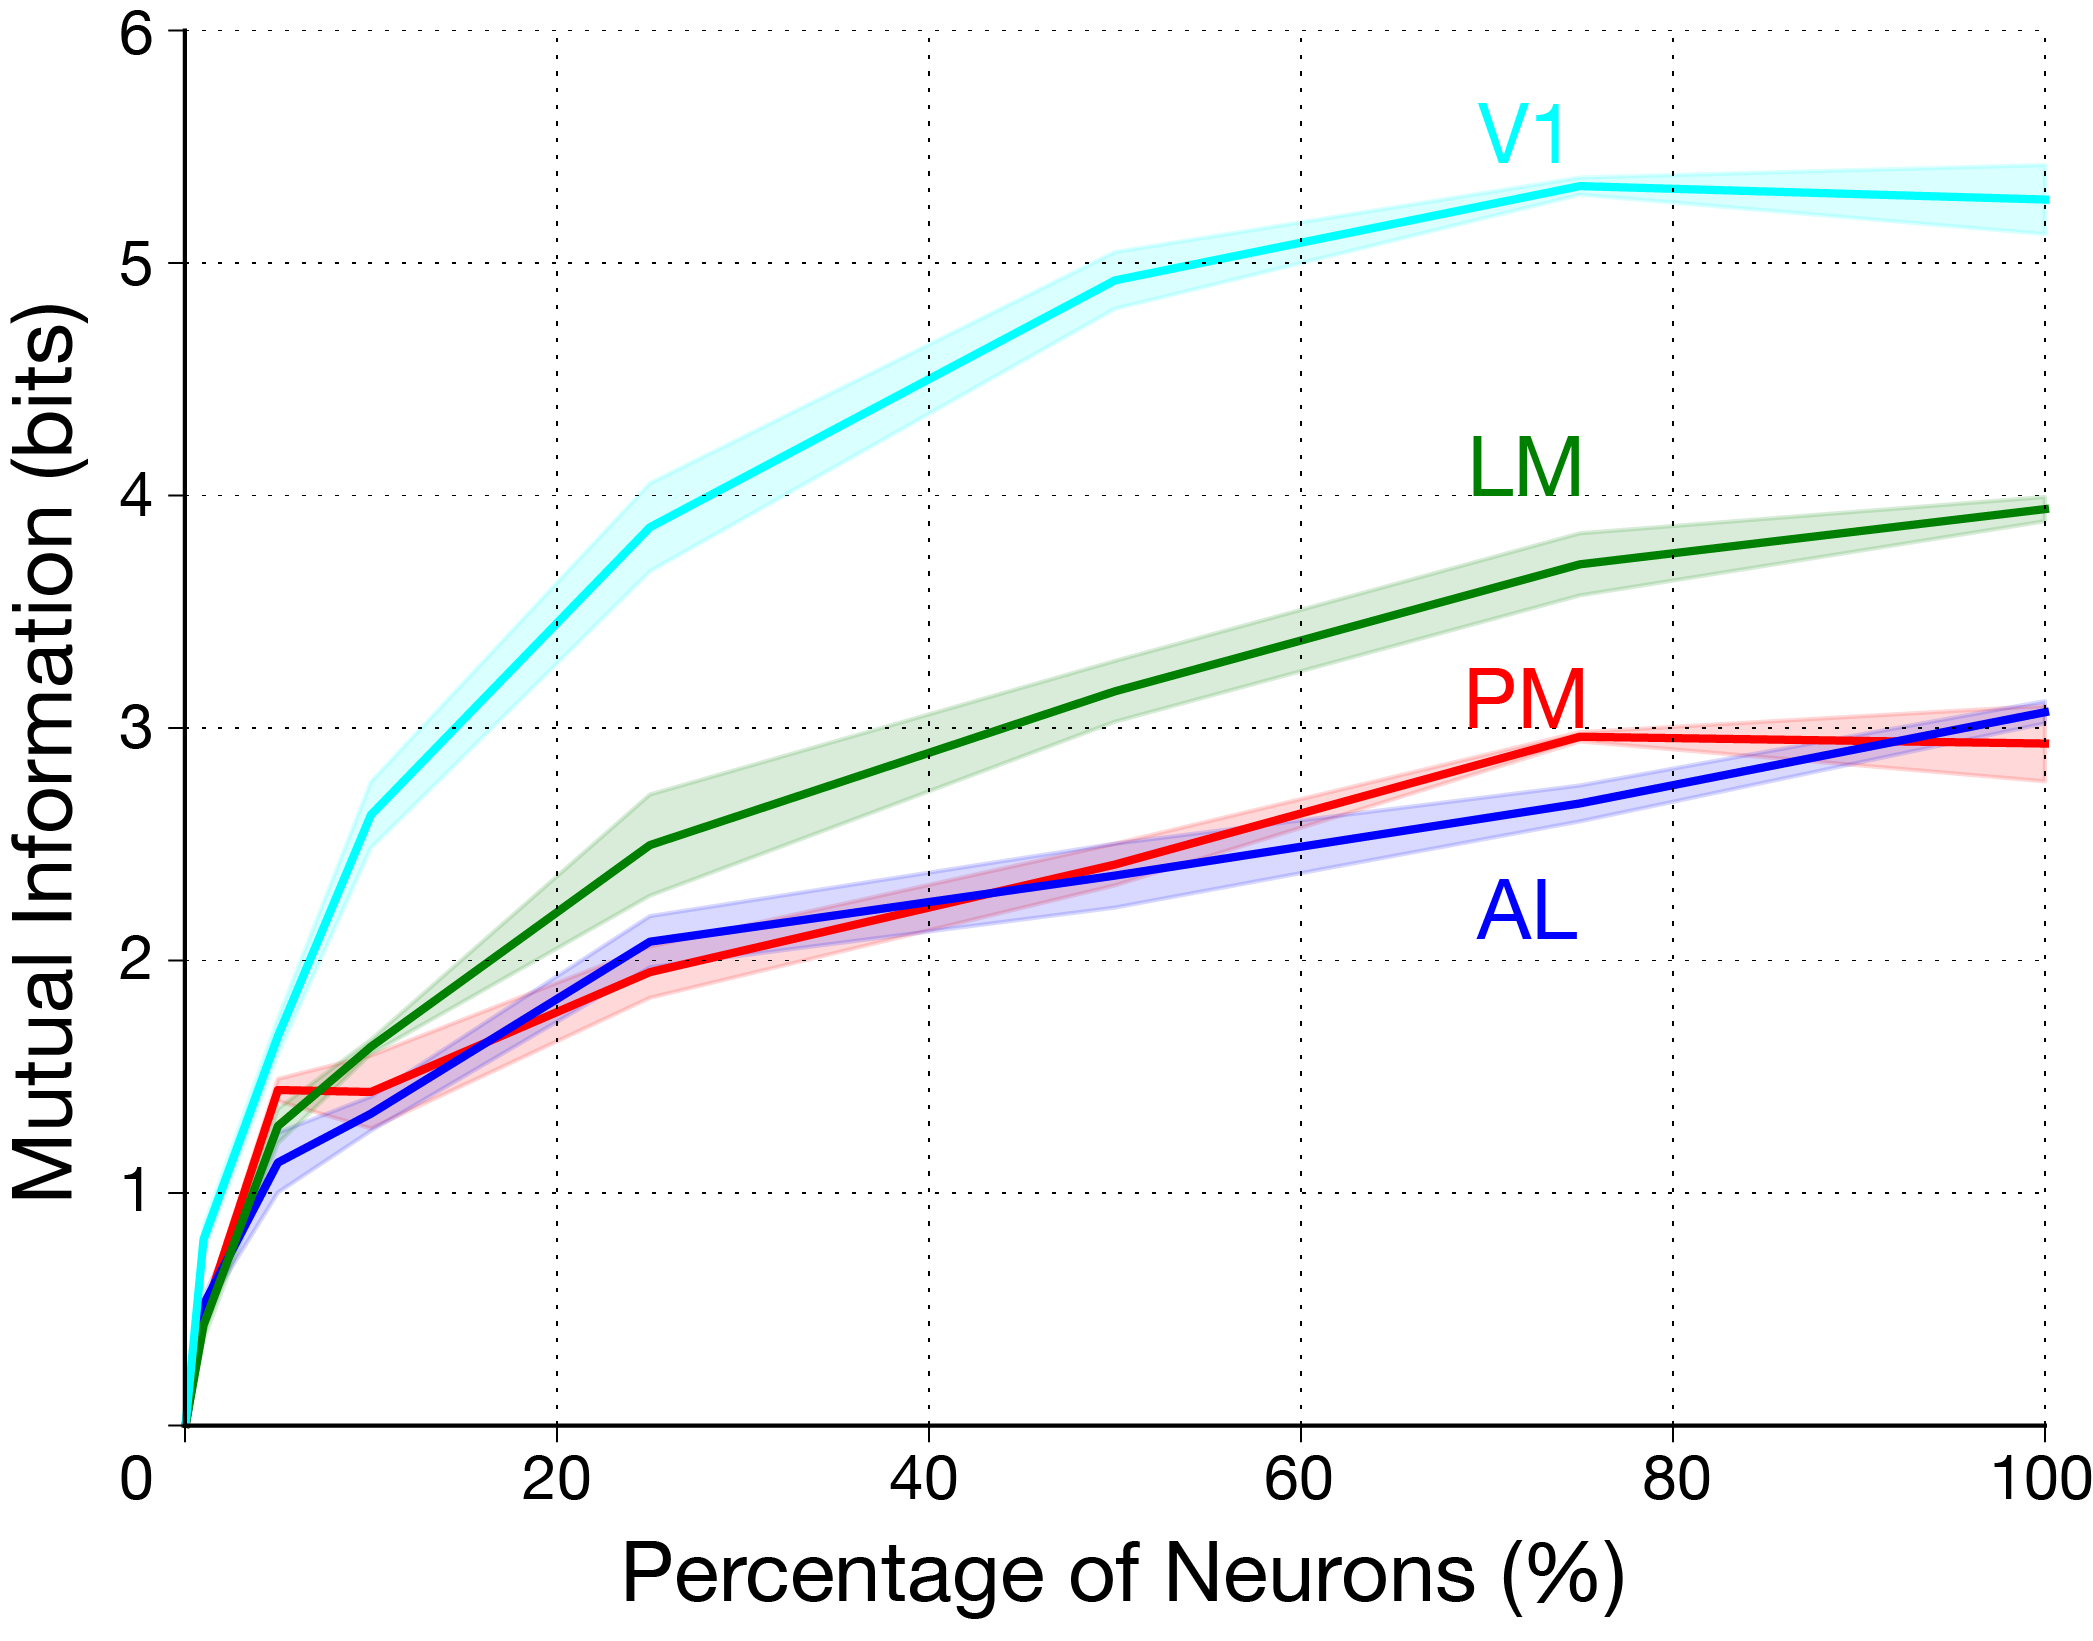
\includegraphics[width=\textwidth]{Figures/chapter5/mutual_info_pop.png}
%    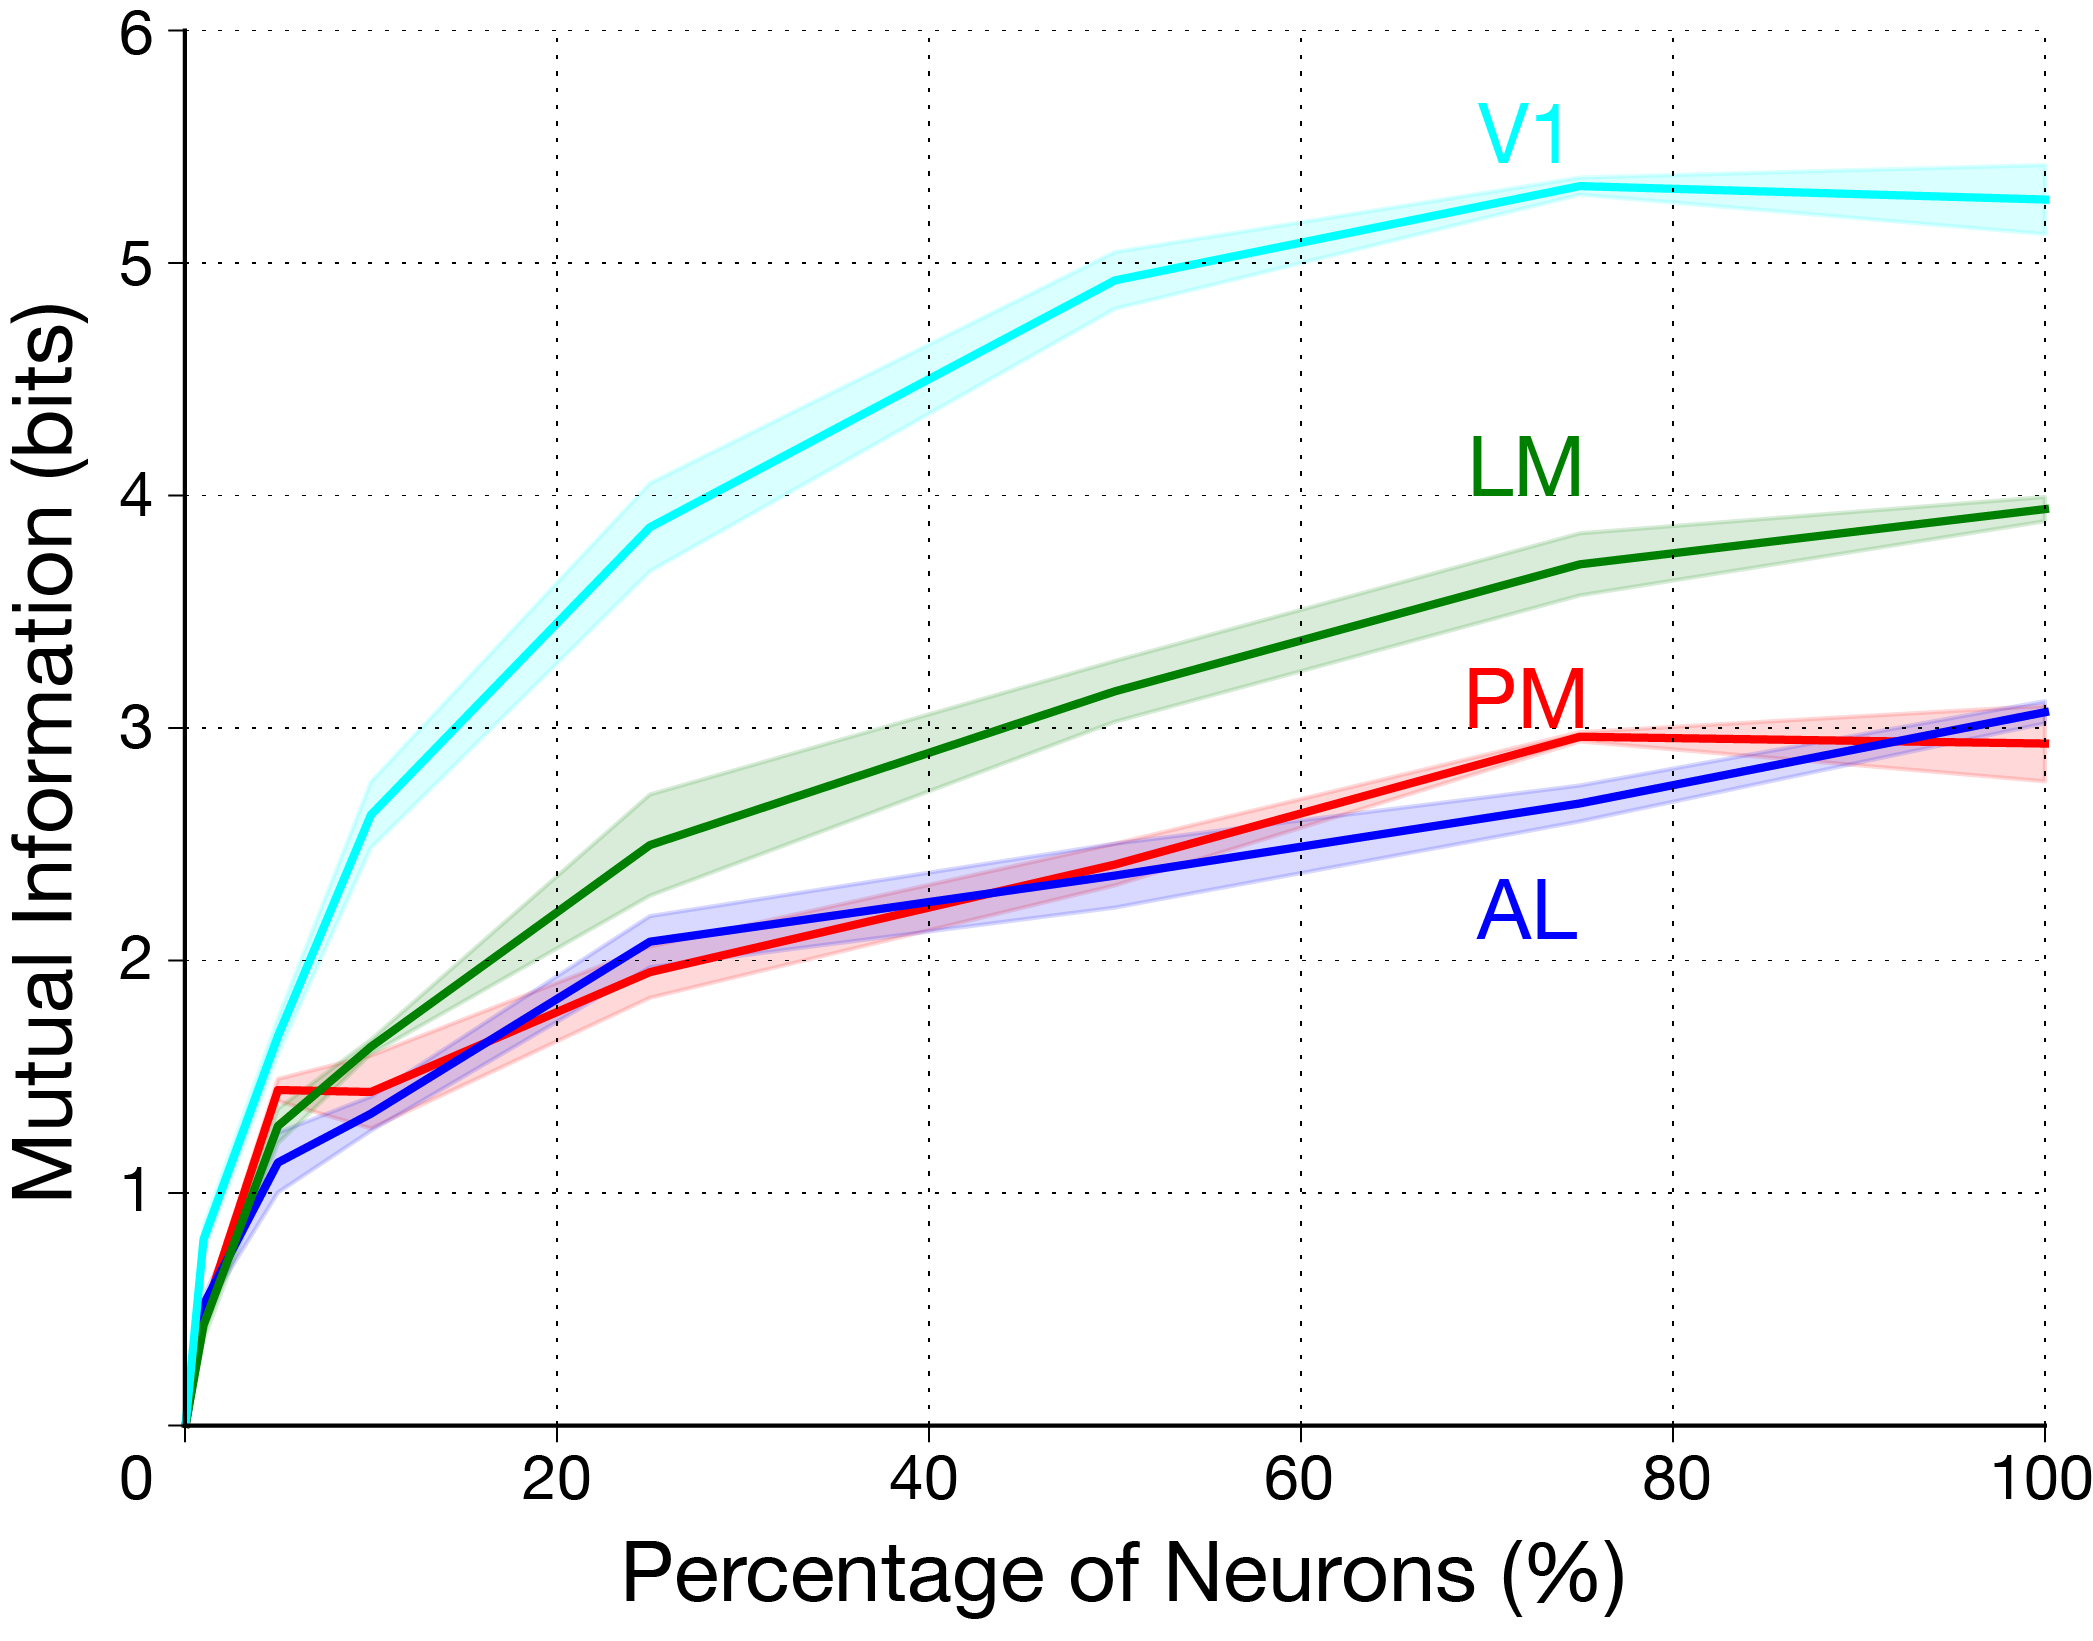
\includegraphics[scale=0.45]{Figures/chapter5/mutual_info_pop.png}
  \caption[Mutual Information Per Population Size]{\textbf{Mutual Information Per Population Size} for individual visual areas. Mutual information calculated as in Equation \ref{eq:mutualinfo}. Solid line represents mutual information. Shaded error bars represent standard error of the mean.}
   \label{fig:mutualinfopop}
\end{figure}
%-----------------------------------------------------------------------------
Next, I evaluated the information content about stimulus identity across time and whether different visual areas might achieve higher accuracy at different times from the stimulus onset. I employed two approaches to evaluate the classifier performance across time. In the first approach, I trained the decoder using the mean response from 200-300ms post-stimulus and tested the classification accuracy at different time points (Figure \ref{fig:decodetime}a). The goal was to assess whether the mean activity activity between 200-300ms also coded information about the stimulus identity at different time periods. In the second approach, I trained and tested the classifier performance at each time point independently (Figure \ref{fig:decodetime} b). Both approaches yielded identical results, with V1 exhibiting greater test accuracy over time compared to higher visual areas.\par 
%-----------------------------------------------------------------------------
\begin{figure}
  \centering
    	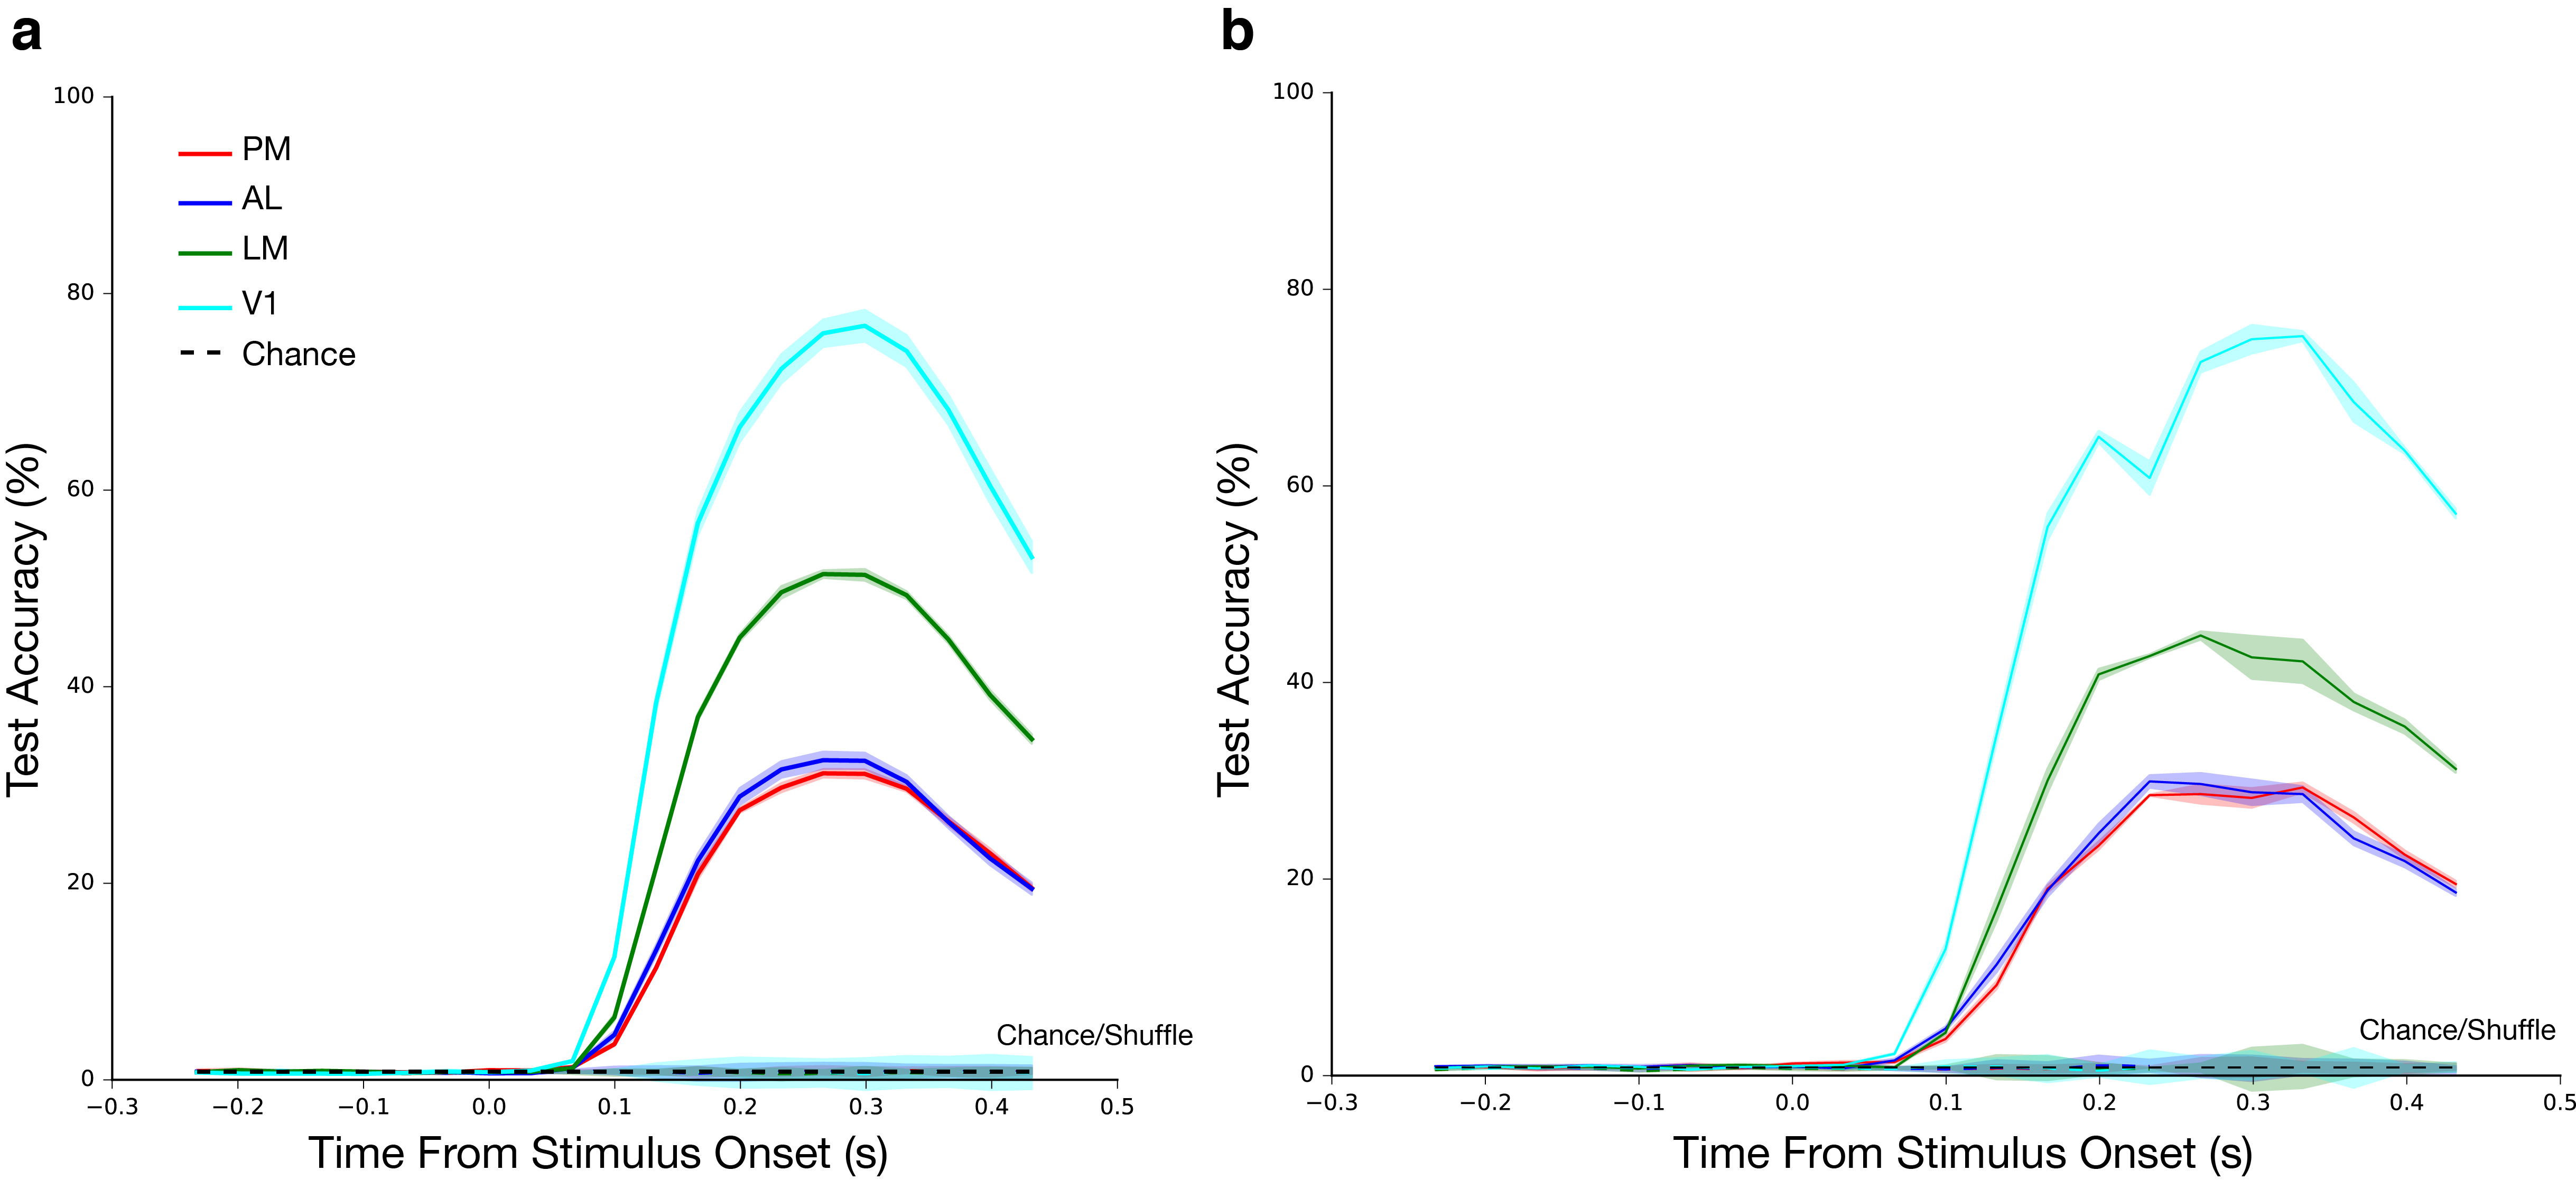
\includegraphics[width=\textwidth]{Figures/chapter5/accuracy_time.png}
%   	\includegraphics[scale=0.3]{Figures/chapter5/accuracy_time.png}
    \caption[Decoder Test Accuracy Over Time]{\textbf{Decoder Test Accuracy Over Time}.(a) Test accuracy of decoder trained with mean activity between 200-300ms post stimulus and tested at each time point. (b) Test accuracy for decoder trained and tested with activity at each time point. Shaded error bars represent standard error of the mean. }
  \label{fig:decodetime}
\end{figure}
%-----------------------------------------------------------------------------
The results described above included all the cells within an area, however, the data can be separated into cortical layers marked by specific cell-type markers (Table \ref{celltable}). I evaluated the performance of cortical layers within an area on decoding natural image identity (Figures \ref{fig:decodecell} and \ref{fig:decodecelltime}). For the analyses, I included 200 neurons per cell type to make an equivalent comparison across different cell types and visual areas. According to the canonical connectivity of principal cells within cortex \parencite{Harris2013}, layer 4 is the prominent recipient of thalamic input although all cortical layers receive thalamic input. Layer 2/3 receives strong projections from layer 4 and sends feedforward projections to higher cortical areas, contralateral cortices, and local projections to layer 5 while layer 5 is the main output layer with local projections to layer 2/3, ipsi- and contra-lateral cortices and the striatum. Layer 5 also receives top-down inputs from higher order brain regions and the thalamus. \par 
%-----------------------------------------------------------------------------
\begin{figure}
  \centering
   \includegraphics[width=\textwidth]{Figures/chapter5/accuracy_cell_type_200_neurons.png}
  \caption[Image Identity Accuracy Per Visual Area Per Layer-Specific Cell Type]{\textbf{Decoder Accuracy Per Visual Area Per Layer-Specific Cell Type}: Test accuracy of classifier trained on average response 200-300ms post-stimulus onset, 200 neurons per cell type. Error bars represent standard error of the mean.}
   \label{fig:decodecell}
\end{figure}
%-----------------------------------------------------------------------------
\begin{figure}
  \centering
   \includegraphics[width=\textwidth,height=0.8\textheight,keepaspectratio]{Figures/chapter5/accuracy_cell_type_time_200_neurons.png}
  \caption[Image Identity Accuracy Per Layer-Specific Cell Type Across Time]{\textbf{Image Identity Accuracy Per Layer-Specific Cell Type Across Time}. Test accuracy of classifier trained with mean response 200-300 ms post-stimulus onset and tested at each time point for each cell type and visual area. 200 neurons per cell type. Shaded error bars represent standard error of the mean.}
   \label{fig:decodecelltime}
\end{figure}
%-----------------------------------------------------------------------------
Although V1 achieved higher decoding performance for each cell type (Figure \ref{fig:decodecell}), there is an intriguing difference between early and higher visual areas. Layer 5 output neurons in early visual areas (V1 \& LM) achieved the highest performance in image identification, whereas in higher visual areas (AL \& PM) layer 2/3 neurons performed better than the layer 5 neurons within their respective areas. It is interesting to consider whether the reversal reflects the flow of information from early to higher visual areas. \par 

\subsection{Decoding Natural Scene Category}
%-----------------------------------------------------------------------------
\begin{figure}
  \centering
     \includegraphics[width=\textwidth]{Figures/chapter5/accuracy_categorization.png}
%    \includegraphics[scale=0.4]{Figures/chapter5/accuracy_categorization.png}
  \caption[Categorization Accuracy: Animal Vs. Non-Animal]{\textbf{Categorization Accuracy: Animal Vs. Non-Animal}. (a) Classifier test accuracy based on average response 200-300ms post-stimulus onset. Gray bars represent shuffled labeled control. Error bars represent standard error of the mean. (b) Test accuracy over time, based on classifier trained on the average response 200-300ms post stimulus onset. Dotted lines represent shuffled labeled control. Shaded error bars represent standard error of the mean.}
   \label{fig:decodecategory}
\end{figure}
%-----------------------------------------------------------------------------
Given the neural responses from visual areas perform well above chance on a natural image identity task, the next question I asked was whether the neural responses could categorize the natural images and whether higher visual area (AL \& PM) would achieve higher performance over early visual areas. The natural images were divided into two groups based on whether an animal was present in the image. A linear classifier was trained for each area to categorize the images into one of two classes. Categorization performance across visual areas was above chance (50\%) and very similar to each, with V1 achieving slightly higher accuracy (Figure \ref{fig:decodecategory}).  

\section{Discussion}
Although the observation that mouse V1 can discriminate natural images is consistent with observations from a previous study from \textcite{Kampa2011}, it is remarkable that V1 \emph{linearly} distinguishes natural images at a greater accuracy than higher visual areas. This observation is in contrast with the seminal view of hierarchical visual processing, which suggests progressive reconstruction of the image from basic low-level representations from the earliest stage to the highest stage in cortex where objects and scene layouts are represented. Embedded in this viewpoint is increased linear separability of the neural representations of the visual image (or object) along the hierarchy \parencite{Rust2010a,Pagan2013}. The primary evidence for hierarchical processing in rodent brains originates from anatomical connectivity \parencite{Coogan1993,Wang2012,DSouza2016}, however it has not yet been established whether a functional visual processing hierarchy exists in the mouse brain in a form similar to the hierarchical and specialized visual processing modules found in the primate brain \parencite{Felleman1991}. \par 

\textcite{Oliva2001} proposed an alternate computational model for scene perception, which states that scenes can be recognized based on holistic (or low-dimensional) descriptions of the scene, also known as the spatial envelope. In this model, scenes can be recognized by linear combinations of low-level features of the image. Further, \textcite{Torralba2003} observed that the spatial properties of the scene and scene category are correlated with second-order statistics of the image and the spatial arrangement of structures in the scene. The model could explain the high decoding accuracy of mouse V1 observed in this chapter. V1 is a low-level feature detector that responds to edges, orientation, and contrast \parencite{Niell2008a,Glickfeld2013b}. Consistent with the computational model proposed by \textcite{Oliva2001}, \textcite{Rikhye2015} recently reported that neurons in mouse V1 use second-order image statistics (ie. spatial correlations) to process natural scenes. \par 

Receptive field (RF) sizes in the mouse visual cortex mirror those found in primates, where RF size increases from early to late visual areas to a size that covers a visual hemifield \parencite{Wang2007}. Since V1 neurons have smaller RFs, V1 could sample the image more densely and resolve more of than image than higher visual areas. Related to the smaller RF sizes in V1, the secondary visual areas have incomplete coverage of visual space \parencite{Garrett2014,Zhuang2017}. Given that individual mouse secondary visual areas could only sample a portion of the visual scene, multiple secondary visual areas might combine resources to gain full access to the visual scene and potentially outperform V1. One way to test this would be to combine neurons from pairs of areas with non-overlapping visual coverage, for example LM \& PM or AL. Then, one could run the classifier analysis combining neurons from areas LM and PM or AL and compare this combined multi-area performance to that of V1.\par 

A major caveat of this study is that the observations are potentially correlated with the quality of the imaging data. The data was collected from each area individually, across different mice. It is not clear whether the quality of the responses is homogeneous across visual areas and depths. For example, higher visual areas PM \& AL may have different imaging quality than V1, which is larger and has more active neurons. The results from this study will greatly benefit from electrical recordings under the same conditions. In the interim, one could degrade the signal quality from V1 by adding noise to the dF/F signal and compare the decode performance. A conceptually similar approach would be to infer spikes via deconvolution methods \parencite{Vogelstein2010}, compare spikes across areas and remove spikes to vary the signal-to-noise ratio. It would also be useful to simultaneously record from multiple visual areas within the same animal.\par 

In the analyses presented in this chapter, I evaluated the decoding accuracy of identifying natural image in awake, passive animals. Future experiments would benefit from testing whether the V1 dominance in natural scene identification persists even when mice are actively engaged in a behavioral task that requires natural scene categorization. Although V1 achieved highest performance in linearly distinguishing between natural images, the neural activity pattern could be more correlated with the features of the image than the behavioral judgment of the mice. Hence, the neural activity patterns in V1 may not exist in a format that is immediately useful for solving the task. One way to test this would be to perform a pairwise correlation between errors made on the task with errors made by the decoder. A high correlation would indicate that the information in a given brain area is used for solving the task. \par 

% Finally, the potential implications of the results of this study is that mouse V1 may not be merely a low-level feature detector,instead it is capable of high-level, and potentially cognitive-level, processing typically designated to higher-order visual brain areas. Examples of higher order processing have been observed in rodent V1 
% This opens up the door for exploring mechanistic level studies of mouse V1 in 
% https://www.ncbi.nlm.nih.gov/pmc/articles/PMC4175492/

% In humans V1 also does significantly above chance, although not the highest

% used greedy approach and pooled neurons across mice, compared to averaging across mice. in future would use more conservative approach.

% Scenes construed as collection of objects 

% V1 sensitive to local texture and spatial frequency content 

% To test whether the high accuracy of mouse V1 is explained solely it being a low-level feature detector, one could interleave presentations of the natural scene images with an inverted copy of each image. The V1 decoder would be trained on the upright images, and tested on the inverted images. If the accuracy of the decoder remains invariant to the scene inversion manipulation, 
% to relies on  are using global attributes of the scene would be to present the mice with the same images, but inverted.  image which would disrupt global scene layout. If performance accuracy is unchanged then V1 picking up local feature information such as texture and spatial freq. V1 would be invariant to the manipulation if simple feature detector.

% Mice have poor spatial acuity, which is slightly improved when they are running. 





% %-----------------------------------------------------------------------------
% \subsection{Neural Representation Similarity Analysis}
% Response pattern dissimilarity matrices
% %-----------------------------------------------------------------------------
% \begin{figure}
%   \centering
%    \includegraphics[scale=0.375]{Figures/chapter5/ssim_matrix_histogram_dssim.png}
%   \caption[Stimulus Set Image Similarity]{\textbf{Stimulus Set Image Similarity} }
%    \label{fig:SSIMhistDSSIM}
% \end{figure}
% %-----------------------------------------------------------------------------
% \begin{figure}
%   \centering
%    \includegraphics[width=\textwidth]{Figures/chapter5/rdm_percentiles.png}
%   \caption[Response Pattern Dissimilarity Matrices]{\textbf{Response Pattern Dissimilarity Matrices} Measured in percentile for  }
%    \label{fig:rdmper}
% \end{figure}
% %-----------------------------------------------------------------------------
% \begin{figure}
%   \centering
%    \includegraphics[scale=0.5]{Figures/chapter5/histogram_rdm.png}
%   \caption[]{\textbf{} }
%    \label{fig:histrdm}
% \end{figure}
% %-----------------------------------------------------------------------------

















 
% Chapter Template

\chapter{Conclusion and Perspectives} % Main chapter title

\label{Chapter6} 

In this thesis, I have demonstrated a quantitative behavioral paradigm for studying temporal accumulation of visual evidence in mice. Mice have been largely underrepresented in studies investigating temporal sensory evidence accumulation, and until recently it remained unclear whether mice could be reliably trained to perform perceptual decision making tasks that require accumulation of sensory evidence over time. Results from cortical manipulation of mouse PPC defined by stereotactic coordinates demonstrated that the accurate performance on the task was depended on cortex, and in particular on normal activity of inhibitory neurons. Furthermore, targeted photoinhibition of secondary visual area AM, located in the mouse parietal cortex area, putatively contributes to evidence accumulation behavior. More precisely, it appears to be involved in guiding contralateral movements. More work is needed to resolve the role of visual area AM as the results are confounded by the artifact of \emph{in vivo} red light stimulation. Finally, I found that population activity of mouse V1 can linearly distinguish between different natural scene images, at a much greater accuracy than other higher order visual areas.\par

Overall, I demonstrated for the first time that a secondary visual area in the mouse contributes to decision making tasks that require evidence accumulation. These experiments lay groundwork for further investigations of the neural circuits that underlie evidence accumulation of visual evidence across time in mouse. Such experiments should focus on using the tools available in mouse to characterize the nature of the neural signals underlying evidence accumulation as well as how this signal influences downstream processes to direct behavior. Below, I outline in detail some of the experiments necessary to address these questions.\par 

The first avenue for future efforts is to develop a computational model of sensory evidence accumulation that quantitatively characterizes the psychophysical behavior of the mice, taking into account the observations identified in Chapter \ref{Chapter2}. A good place to begin would be with the extended drift diffusion accumulator model developed by \parencite{Brunton2013}. The Brunton model uses trial-by-trial stimulus information to estimate the noise associated with the evidence accumulator. Among the main features of the model is that estimates the accumulator noise separately from the noise associated with the incoming sensory evidence. Included in the model are parameters that account for sensory adaptation, which would be useful in determining to what extent subjects use a brightness in solving the task. The model could also be used to determine the optimal shape of the psychophysical kernel, and whether mice are accumulating evidence optimally. More interestingly, the computational model could generalize to multiple evidence accumulation tasks that use pulsatile sequences. Currently there is not a consensus on sensory evidence accumulation tasks and it is unclear whether the brain treats has a generalized solution for solving such tasks. For instance the task developed in this thesis utilizes a single stream of evidence that is non-spatial, however, several paradigms have also used two independent spatially-localized streams  \parencite{Sanders2012,Brunton2013,Marcos2016,Katz2016}. With a general computational framework, it would be interesting to compare the different modes (one vs two stream) of evidence accumulation and different different species trained on the same task. \par 

An open avenue to explore is the role of the corticostriatal connection, namely the prominent projection from area AM to striatum. Although the striatum has been implicated in perceptual decision making \parencite{Ding2010,Ding2013}, few studies have investigated corticostriatal circuits in the context of perceptual decision making. Previous work by \textcite{Znamenskiy2013b} demonstrated that corticostriatal neurons in auditory cortex can selective bias and drive behavioral decisions. It is not known whether this generalizes to striate or extrastriate visual cortices. The striatum, and other subcortical motor areas, is interesting because it predates the neocortex, is coupled to motor circuits in the brain stem, and receives sensory inputs from multiple brain areas. Hence it is likely an important hub for understanding how sensory and perceptual information is converted into action. \par

Further work is needed to understand the functional roles of mouse secondary visual areas and their involvement in perceptual decision making behavior. The approach used in this thesis, targeted a single area across multiple mice. Although this low-throughput approach could be scaled up by running large cohorts of animals in parallel, each with an inactivation target to a particular visual area, it is not ideal for understanding how multiple areas work in concert to generate behavior. Hence, future work could leverage large-scale tools for perturbing and/or recording neural activity from multiple brain areas simultaneously (or combinatorially). For example, the paradigm described in this thesis can be optical neural recording techniques such as head-mounded microscopes \parencite{Ghosh2011} or multi-area fiber photometry \parencite{Kim2016}. With the right configuration, the multi-area fiber photometry system could also be used for photoinhibition. Alternatively, an analogous head-restrained version of the task \parencite{Marbach2016} could be implemented and combined with patterned photoinhibition \parencite{Dhawale2010,Guo2014a}, widefield imaging \parencite{Wekselblatt2016}, and/or cellular-level mesoscale imaging \parencite{Stirman2016a,Sofroniew2016} in behaving mice. The possibilities are endless.

In summary, the underlying theme of this thesis was to understand how sensory and perceptual information is transformed into categorical decisions and ultimately actions. Perhaps for the first time in systems neuroscience, we are living in an age of abundant tools for probing, manipulating, and monitoring neural circuit components and at the center of the technological revolution is the mouse. With carefully designed behavioral paradigms and stimuli that harness evolved features of their sensory systems, mice are capable of performing complex behavioral task that require cortical machinery. Therefore, now is the time to leverage existing behavioral paradigms and tools to discover unknown computational algorithms implemented in biological tissue, and ultimately, inspire the design of the next generation of intelligent machines.


 
%\include{Chapters/Chapter7} 

%-------------------------------------------------------------------------
%	THESIS CONTENT - APPENDICES
%-------------------------------------------------------------------------

\appendix % Cue to tell LaTeX that the following "chapters" are Appendices

% Include the appendices of the thesis as separate files from the Appendices folder
% Uncomment the lines as you write the Appendices

% Appendix A

\chapter{Materials and Methods} % Main chapter title

\label{AppendixA} % Change X to a consecutive number; for referencing this chapter elsewhere, use \ref{ChapterX}

\section{Animal Subjects}
All animal procedures and experiments were approved by the Cold Spring Harbor Laboratory Animal Care and Use Committee. Experiments were conducted with female or male mice between the ages of 6-25 weeks. Mouse strains were either C57BL/6J or SV129 background. Trangenic mice used included Ai93/Emx-tTA/CamKII $\alpha$-tTA (GCaMP6f), Ai95/Emx-cre (GCaMP6f), Gad2-Cre, and PV-IRES-Cre. \\
For behavioral performance comparison, male Long Evan rats (6 weeks, Taconic) were also used. 

\section{Headbar Implantation and Skull Preparation}
For retinotopic mapping measurements, mice were implanted with a custom titanium headbar. Mice were anesthetized with isoflurane (2\%) mixed with oxygen and secured onto a stereotaxic apparatus. Body temperature was maintained at 37 $^{\circ}$ C with a rectal temperature probe. The eyes were lubricated with eye ointment before the start of the surgery, followed by subcutaneous injection of analgesia (Meloxicam, 2mg/kg) and antibiotic (Enrofloxacin, 2mg/kg). Fur on the scalp was removed with hair clippers and Nair (Sensitive Formula with Green Tea), followed by betadine (5\%) swab. Lidocaine (100 $\mu $L) was injected underneath the scalp before removing the scalp. The skull was cleaned with saline and allowed to dry. A generous amount of vetbond tissue glue (3M) was then applied to seal the skull. Once the vetbond was dry, the headbar was secured with Metabond (Parkwell) and dental acrylic. Mice were allowed 3 days to recover before retinotopic mapping. 
 
\section{Window Implantation} 
Window implantation is optional for retintoptic mapping, as the mouse skull is translucent. This procedure requires sterile technique and is typically done in conjunction with the headbar implant. The optical window implantation procedure was adopted from \textcite{Goldey2014}. Briefly, the mouse was anesthetized with isoflurane and secured onto a stereotaxic instrument (Kopf). The eyes were lubricated with eye ointment before the start of the surgery, and the mouse was administered subcutaneous injections of Dexamethasone (4 mg/kg) to prevent swelling of the brain, Meloxicam (2mg/kg), and Enrofloxacin (2mg/kg). The scalp and skull was prepared using the same technique described above. Vetbond tissue glue was applied to skull, followed by a unilateral craniotomy using a disposable biopsy punch (Milltex) of the desired size (4 mm). Three round glass coverslips (2-4mm and 1-5mm, Warner Scientific) glued together with optical glue (Norland Optical Adhesives, \#71) were used to seal the craniotomy with Vetbond. Post-operative analagesia (Meloxicam, 2mg/kg) was administered daily for 5 days following the surgery.  Mice were allowed 5-10 days to recover before retinotopic mapping.  

\section{Retinotopic Mapping}
Retinotopic mapping was performed in awake headfixed animals using one of two procedures, episodic \parencite{Gias2005,Andermann2011} or periodic (Fourier) stimulation \parencite{Kalatsky2003,Garrett2014,Juavinett2016}. For episodic stimulation, spatially restricted drifting gratings (25-40$^{\circ}$ in diameter) were presented to the hemifield contralateral to the window implant or exposed skull. A typical trial proceeded in the following sequence: 4s blank, 4s stimulus, and 4s blank. Each trial was followed by a 6 to 8s inter trial interval. A gray screen was presented during blank periods, and the the stimulus was presented on a gray background. Each stimulus location was repeated 20-80 times. \\
For periodic (Fourier) stimulation, a narrow bar (5-10 $^{\circ}$) was drifted across the four cardinal directions of the screen. Presented within the drifting bar was a flickering checkerboard pattern (12 $^{\circ}$ checks, 5Hz). One trial consisted of 11 sweeps of the bar in 22 secs in one of the four cardinal directoins, however the the first cycle was discarded because it typically introduced stimulus onset transients. Each trial was repeated 15 times for each direction. The monitor was placed in contralateral visual hemifield to imaging hemisphere, positioned at an angle of 77 $^{\circ}$ from the midline of the mouse and a distance of 15 cm.The procedures for periodic retinotopic mapping were adopted from \parencite{Juavinett2016}. Imaging data was acquired at frame rates between 5 to 50 fps. 

\section{Behavioral Training}
Before behavioral training, mice were gradually water restricted over the course of a week. Mice were weighed daily and checked for signs of dehydration throughout training period. Mice that weighed less than 80\% of their original pre-training weight were supplemented with additional water. Behavioral training sessions typically lasted 1-2 hours, daily, in which mice typically harvested at least 1 mL of water. Mice rested on the weekends. If a mouse failed to harvest at least 0.4 mL on two consecutive days, the mouse was supplemented with additional water.\par
Animal training took place in sound isolation chamber, which contained a three-choice port box. The mouse would poke into the center port to initiate trials and deliver the stimulus. Given the stimulus, the animal reported its choice on either the left- or right-side port. In the first training stage, mice learned to wait for at least 1100 ms at the center port before reporting their decision. This behavior was shaped by rewarding the mice at the center port (0.5 $\mu $L) and gradually increasing the minimum wait duration from 25 ms to 1100 ms over the course of 1-2 behavioral sessions. Without center reward, this stage typically took 10-12 sessions to learn. During the first stage of training, the stimulus is played and the reward (2 $\mu$L) is automatically dispensed at either the left or right side depending on the stimulus. In this phase the mouse is not punished for an incorrect first choice.  In the second stage of training, the mouse learns to discriminate the stimulus and is required to make the correct choice on the first attempt. Initially, mice are biased during this stage and several anti-bias methods are employed to correct the bias, such as physically obstructing access the biased port, changing the reward size, or proportion of left vs right trials. The mouse is considered trained once they are unbiased, performing above chance, and experiencing all stimulus strengths.\par
Trial type, stimulus and reward delivery, control, and data collection was performed through a MATLAB interface and Arduino-powered device called BPod (SanWorks LLC).\par 

\section{Stimulus Generation}
The stimulus consists of a sequence of 20 ms pulses of light from a LED panel (Ala Scientific). The inter-pulse intervals are randomized from a uniform or exponential distribution. In earlier experiments (fixed interval), the intervals were drawn from a uniform distribution of 50 or 100 ms, and each pulse was 15 ms. In the fixed interval stimulus, the event rates were between 9 to 16 flashes/s with a category boundary at 12.5 flashes/s. For the exponential interval stimulus, the minimum inter-pulse interval was 20 ms, and the maximum interval was determined by the number of flashes for a given stimulus. The number of flashes were between 4-20 flashes/s. The stimulus was created using 25 fixed time bins, each 20ms in duration. A Poisson coin was flipped to determine whether an event (flash) would occur in each bin. Each fixed time bin was followed by an empty 20ms time bin. 
\subsection{Brightness Manipulation}
Each 20ms flash pulse was generated by a half-wave rectified sinusoidal signal thresholded at the peaks and with a base frequency of 200Hz. This approach effectively controls the total LED on-time or the "density" of the 20ms pulses. It is similar to pulse-width modulation technique used to control LED brightness. During normal sessions, the base frequency is multiplied by a brightness factor, which is kept constant across sessions. In the first brightness manipulation experiment, the normal brightness factor was either halved or doubled on 5\% of trials to produce the "dimmer" and "brighter" conditions. In the second brightness manipulation experiment, the normal brightness factor was inversely scaled with the flash rate such that the brightness factor was normalized by the quotient of the flash rate of the current trial and the lowest flash rate (4 flashes/s). This manipulation was introduced on 5\% of trials.  

\section{Chemogenetics Experiments}
Mice (Gad2-IRES-cre) were injected with AAV8-hSyn-DIO-hm4Di-mCherry into stereotactic mouse PPC \parencite{Harvey2012}. Approximately 200nL of virus was injected in both hemispheres at 200 $\mu$m below the surface of the brain.  The mice were allowed to 3 days to recover before behavioral training. \\
CNO (Sigma or Enzo Life Sciences) was diluted to a final concentration of 0.5mg/ml in saline and DMSO, and stored in aliquots of 0.4ml in the -80 $^\circ$ C. Each CNO aliquot was used only once after thawing, Mice were administered a dosage of 2mg/kg (or 100 $\mu$ L/25g mouse) of CNO or an equivalent volume of saline (0.9\%). Care was taken to ensure that there was at least two-three days between CNO treatments to allow full recovery and stabilization of behavior. 

\section{Survival Blood Collection via Lateral Tail Vein (Mouse)}
Mouse was placed on warm heating pad. The temperature should not exceed 85-90 $^\circ$ F. The mouse was then placed in a plastic restrainer.The tail was cleaned with 70\% ethanol. The lateral tail vein was nicked With a \#11 scalpel blade. Blood(15-30 $\mu$L was collected into a receptacle. Excess blood was cleaned up with Kimwipe and the wound sealed with Vetbond. The blood sample was centrifuged, and the blood plasma extracted. The plasma was submitted to and analyzed by the CSHL Proteomics Facility. 

\section{Optogenetic Inactivation}
For Jaws inhibition experiments, mice were injected with AAV8-hSyn-Jaws-KGC-GFP-ER2 (Group 1) or AAV8-CamKII-Jaws-KGC-GFP-ER2 (Group 2) into area AM identified by retinotopic mapping. Virus injections were performed using Drummond Nanoject III, which enables automated delivery of small volumes of virus. To minimize virus spread, the Nanoject was programmed to inject slowly: six 30 nL boluses, 60 s apart, and each bolus delivered at 10 nL/sec.
Approximately 180nL of virus was injected at multiple depths ($\sim$200 and $\sim$500 $\mu $m) below the brain surface. Following the virus injection, 200 $\mu$m fiber (metal ferrule, ThorLabs) was implanted above the injection site. The optical fiber was secured onto the skull with vitrebond, metabond, and dental acrylic. The animals was allowed at least 3 days to recover before behavioral training. \\
A red 640nm fiber-coupled laser (OptoEngine) was used for inactivation. Experiments were conducted with multiple laser power levels: 0.5, 1, and 2 mW. One power level was used per session. On inactivation sessions, laser light was externally triggered using a PulsePal (Sanworks LLC) device. The laser stimulation pattern was a square pulse (1 second long) followed by a linear ramp (0.25s), which began at the onset of the stimulus. Stimulation occurred on 25\% of trials. 





\chapter{Supplementary Data Figures} % Main appendix title

\label{AppendixB} 

\begin{figure}
  \centering
  	\includegraphics[width=\textwidth,height=\textheight,keepaspectratio]{Figures/chapter2/psychKernel_individualmice.png}
  \caption[Psychophysical Kernels of Individual Mice]{\textbf{Psychophysical Kernels of Individual Mice}. Data (blue) and shuffle control (gray). Shaded areas represent standard error of estimated coefficients.}
   \label{fig:allkernels2}
\end{figure}
%--------------------------------------------------------------------------

\begin{figure}
  \centering
  	\includegraphics[width=\textwidth,height=\textheight,keepaspectratio]{Figures/chapter2/rat_kernel.png}
  \caption[Psychophysical Kernels of Rats Trained on Visual Flashes Task]{\textbf{Psychophysical Kernels of Rats Trained on Visual Flashes Task}. Data (blue) and shuffle control (gray). Shaded areas represent standard error of estimated coefficients.}
   \label{fig:ratkernel}
\end{figure}
%--------------------------------------------------------------------------
\begin{figure}
  \centering
   \includegraphics[width=\textwidth]{Figures/chapter4/kppc1_harvey_ppc_injections.png}
  \caption[Retinotopic Map of Stereotactic Mouse PPC]{\textbf{Retinotopic Map of Stereotactic Mouse PPC}. GCaMP6m virus was injected into stereotactic coordinates for mouse PPC (2mm posterior, 1.7mm lateral,\parencite{Harvey2012}) in the right hemisphere (a) Locations of drifting grating stimulus on monitor. The monitor was positioned at 90$\deg$ relative to the mouse (b) GCaMP6m virus expression through window (yellow). (c) Overlay of response maps from 4 stimulus locations. (d) Overlay of GCaMP6 response map with window and injection site (x).}
   \label{fig:ppcgcamp}
\end{figure}

% kPPC1 Sept06-2016
% injected aav1-syn-gcamp6m into Harvey PPC coordinates
% 2mm posterior,1.7mm lateral to bregma
% performed widefield imaging of gcamp6 signal 
%-----------------------------------------------------------------------------

\begin{figure}
  \centering
   \includegraphics[width=\textwidth,height=0.8\textheight]{Figures/chapter4/jaws_AM_group1_individualPMFs.png}
  \caption[Area AM Group 1 Individual Psychophysical Data]{\textbf{Area AM Group 1 Individual Psychophysical Data}. Photoinhibition at 32 mW/mm$^{2}$. Circles represent the subject's behavioral response during laser OFF (black) and laser ON (red) trials. Solid line represents the psychometric function fit to cumulative Normal (Equation \ref{eq:normalpmf}). Error bars represent Wilson Binomial (95\%) confidence intervals. }
   \label{fig:AMgroup1individual}
\end{figure}
%-----------------------------------------------------------------------------
\begin{figure}
  \centering
   \includegraphics[width=\textwidth]{Figures/chapter4/GLMM_PMFS_32mWpermmsq_group1.png}
  \caption[Psychometric GLMM Fit - AM Group 1 - 32 mW/mm$^{2}$]{\textbf{Psychometric GLMM Fit - AM Group 1 - 32 mW/mm$^{2}$} for each mouse (n=6). Circles represent the subject's response data for laser OFF (black) and laser ON (red) conditions. The solid line represents the GLMM fit.}
   \label{fig:AMg1GLMM32}
\end{figure}
%-----------------------------------------------------------------------------
\begin{figure}
  \centering
   \includegraphics[width=\textwidth]{Figures/chapter4/jaws_controls_individualPMFs.png}
  \caption[Control Group Individual Psychophysical Data ]{\textbf{Control Group Individual Psychophysical Data} from two mice (kg15 and kg16) under two conditions. (a,c) Without the masking red light. Laser stimulation irradiance 32 mW/mm$^{2}$. (b,d) Masking red lights present in the behavior booth. Laser stimulation irradiance 64 mW/mm$^{2}$. Circles represent the subject's behavioral response during laser OFF (black) and laser ON (red) trials. Solid line represents the psychometric function fit to cumulative Normal (Equation \ref{eq:normalpmf}). Error bars represent Wilson Binomial (95\%) confidence intervals. }
   \label{fig:ctrlindividual}
\end{figure}
%-----------------------------------------------------------------------------
\begin{figure}
  \centering
   \includegraphics[width=\textwidth,height=0.75\textheight,keepaspectratio]{Figures/chapter4/jaws_controls_house_red_full_rates_PMFs.png}
  \caption[Control Group Psychophysical Data - More Flash Rates]{\textbf{Control Group Psychophysical Data - More Flash Rates} (a) Pooled psychophysical data from two mice (b) kg15 and (c) kg16 with more flash rates. Masking red light present during sessions. Laser stimulation irradiance at 64 mW/mm$^{2}$. Solid line represents the psychometric function fit to cumulative Normal (Equation \ref{eq:normalpmf}). Error bars represent Wilson Binomial (95\%) confidence intervals. }
   \label{fig:ctrlpmfs}
\end{figure}
%-----------------------------------------------------------------------------
\begin{figure}
  \centering
   \includegraphics[width=\textwidth,height=0.8\textheight,keepaspectratio]{Figures/chapter4/GLMM_PMFS_controls.png}
  \caption[Psychometric GLMM Fit - Control Group]{\textbf{Psychometric GLMM Fit - Control Group} for n = 2 mice (a) No masking red light, laser stimulation at 32 mW/mm$^{2}$ (b) Masking red light present, laser stimulation irradiance at 64 mW/mm$^{2}$. Circles represent the subject's response data for laser OFF (black) and laser ON (red) conditions. The solid line represents the GLMM fit. }
   \label{fig:glmmcontrolpmfs}
\end{figure}

%-----------------------------------------------------------------------------
\begin{figure}
  \centering
   \includegraphics[width=\textwidth,height=0.8\textheight,keepaspectratio]{Figures/chapter4/glmm_pmf_effects_controls.png}
  \caption[Psychophysical Effects of \emph{in vivo} red light stimulation on control group]{\textbf{Psychophysical Effects of \emph{in vivo} Red Light Stimulation - control Group} (a) Effect of \emph{in vivo} red light stimulation on the slope of the psychometric function ($\beta_{evidence:opto}$) in the presence and absence of masking red light. Irradiance for each condition is 32 and 64 mW/mm$^{2}$ respectively. Error bars represent 95\% confidence interval. Asterisks mark statistically significant (p<0.05) coefficients. (b) Choice bias as defined in Equation \ref{choicebias}. Choice bias error bars represent 95\% confidence intervals estimated by error propagation.}
   \label{fig:glmmcontrol}
\end{figure}
%-----------------------------------------------------------------------------
\begin{figure}
  \centering
   \includegraphics[width=\textwidth]{Figures/chapter4/glmm_PMFS_16mWmm2.png}
  \caption[Psychometric GLMM Fit - AM Group 2 - 16 mW/mm$^{2}$]{\textbf{Psychometric GLMM Fit - AM Group 2 - 16 mW/mm$^{2}$} for each mouse (n=8). Circles represent the subject's response data for laser OFF (black) and laser ON (red) conditions. The solid line represents the GLMM fit. Top row is group 2A and bottom row is group 2B. }
   \label{fig:amGLMM16}
\end{figure}
%-----------------------------------------------------------------------------
\begin{figure}
  \centering
   \includegraphics[width=\textwidth]{Figures/chapter4/glmm_PMFS_32mWmm2.png}
  \caption[Psychometric GLMM Fit - AM Group 2 - 32 mW/mm$^{2}$]{\textbf{Psychometric GLMM Fit- AM Group 2 - 32 mW/mm$^{2}$} for each mouse (n=8). Circles represent the subject's response data for laser OFF (black) and laser ON (red) conditions. The solid line represents the GLMM fit. Top row is group 2A and bottom row is group 2B.}
   \label{fig:amGLMM32}
\end{figure}
%-----------------------------------------------------------------------------
\begin{figure}
  \centering
   \includegraphics[width=\textwidth]{Figures/chapter4/glmm_PMFS_64mWmm2.png}
  \caption[Psychometric GLMM Fit - AM Group 2 - 64 mW/mm$^{2}$]{\textbf{Psychometric GLMM Fit - AM Group 2 - 64 mW/mm$^{2}$} for each mouse (n=7). Circles represent the subject's response data for laser OFF (black) and laser ON (red) conditions. The solid line represents the GLMM fit. Top row is group 2A and bottom row is group 2B. }
   \label{fig:amGLMM64}
\end{figure}
%-----------------------------------------------------------------------------







%\include{Appendices/AppendixC}

%-------------------------------------------------------------------------
%	BIBLIOGRAPHY
%-------------------------------------------------------------------------

\printbibliography[heading=bibintoc]

%-------------------------------------------------------------------------

\end{document}  
